\documentclass{book}
\usepackage[utf8]{inputenc}
\usepackage[english]{babel}
\usepackage[T1]{fontenc}
\usepackage[utf8]{inputenc}
\usepackage{array}
\usepackage{mathtools}
\usepackage{natbib}
\usepackage{graphicx}
\usepackage{amsfonts}
\usepackage{amsmath}
\usepackage{polynom}
\usepackage{gensymb}
\usepackage{pgfplots} 
\usepackage{tikz}
\usepackage{listings}
\usepackage{gauss}
\usepackage{comment}
\usepackage{bbm}
\usepackage[top=1in,bottom=1in,right=1in,left=1in]{geometry}
\pgfplotsset{width=10cm,compat=1.9}
\DeclareMathOperator{\Ima}{Im}
\DeclareMathOperator{\Rang}{rang}

\title{Masters Programme in Computer and Information Engineering}
\author{Anton Augustsson}
\date{June 2020}


\begin{document}

\maketitle
\newpage
\tableofcontents


\chapter{Basic Course in Mathematics}

\newpage

\begin{multicols}{2}
\section{Basic}
\subsection{Mängder}
\begin{align*}
  &\quad \text{Naturliga tal: } \mathbb{N} = \{ 1, 2 , 3 ...  \} \\
  &\quad \text{Heltal: }\mathbb{Z} = \{... -2, 1, 0, 1, 2 ...  \} \\
  &\quad \text{Rationella tal: }\mathbb{Q} = \{ \frac{a}{b} | a,b \in \mathbb{Z}, b \\
  &\quad \text{Irrationella tal: }\mathbb{P} = \frac{\mathbb{R}}{\mathbb{Q}}eller \{ x | x \in \mathbb{R}, x \notin \mathbb{Q} \} \\
  &\quad \text{Reella tal: }\mathbb{R} =  \mathbb{P} \cup \mathbb{Q} \\
\end{align*}


\subsection{Potenslagar}
\begin{align*}
  &\quad (\frac{a}{b})^{-3} = (\frac{b}{a})^{3}\\
  &\quad \sqrt{a} = a^{\frac{1}{2}} \\
\end{align*}


\subsection{Logaritmer}
%\begin{align*}
%  &\quad y = a^x \Leftrightarrow \log_a(y) = x  \\
%  &\quad 0<a<1 \text{ och } 1<a \text{ ger olika grafer} \\
%\end{align*}
%
%\begin{tikzpicture}
%\begin{axis}[
%    axis lines = left,
%    xlabel = $x$,
%    ylabel = {$f(x)$},
%]
%%Below the red parabola is defined
%\addplot [
%    domain=-5:5, 
%    samples=100, 
%    color=red,
%]
%{2^x};
%\addlegendentry{$2^x$}
% \addplot [
%    domain=-5:5, 
%    samples=100, 
%    color=black,
%]
%{0.5^x};
%\addlegendentry{$0.5^x$} 
%\end{axis}
%\end{tikzpicture}


\textbf{Logaritmlagar:}\par
Va vaksam över när a<0 då är logarytmen odefinerad. 
\begin{align*}
  &\quad \text{(1): } b = a^x \Leftrightarrow \log_a(b) = x  \text{ för: } a>0, b>0, a \ne 1  \\
  &\quad \text{(2): } \log_a(\frac{b}{c}) = \log_a(b) - \log_a(c) \\
  &\quad \text{(3): } \log_a(b*c) = \log_a(b) + \log_a(c) \\
  &\quad \text{(4): } \log_a(b^d) = d\log_a(b) \\
  &\quad \text{(5): } \log_a(b) = \frac{\log_f(b)}{\log_f(a)} \\
  &\quad \text{(6): } \log_a(a) = 1 \\
  &\quad \text{(7): } \log_a(1) = 0 \\
  &\quad \text{(8): } a^{\log_a(x)} = x \\
  &\quad \text{(9): } \log_{a^c}(b) = \frac{1}{c} \log_a(b) \\
\end{align*}

\subsection{Tillvägagångs sätt}
\begin{equation}
\log_3(x) + \log_x(\frac{1}{27}) = 2
\end{equation}

\subsubsection{Lösning}
\begin{align*}
  &\quad \log_3(x) - 3 \log_x(3) = 2 \\
  &\quad  \log_3(x) - 3 \frac{\log_3(3)}{\log_3(x)} = 2 \\
  &\quad  \log_3(x) - 3 \frac{1}{\log_3(x)} = 2 \\
  &\quad  \log_3(x)^2 - 3 = 2 \log_3(x) \\
  &\quad  y = \log_3(x)^{2} \\
  &\quad  y^2 - 2y- 3 = 0 \\
  &\quad  \text{pq-formeln: } y= 1 \pm \sqrt{4} = 1 \pm 2 \\
  &\quad  \log_3(x) = 3 \Leftrightarrow x = 3^3 = 27 \\
  &\quad  \log_3(x) = -1 \Leftrightarrow x = 3^{-1} = \frac{1}{3} \\
\end{align*}


\subsection{Intervall}
\begin{equation}
[ \, a, b ] \, = \{ x | a \leq x \leq b \}
\end{equation}

\begin{equation}
[ \, a, \infty [ \,
\end{equation}
\begin{equation}
] \, -\infty, \infty [ \,
\end{equation}

\subsection{Tillvägagångs sätt}
\begin{equation}
\frac { 2 } { x - 3 } < \frac { 5 } { x }
\end{equation}


\subsubsection{Lösning}
\begin{align*}
&\quad \frac{ 2 }{ x - 3 } - \frac{ 5 }{ x } < 0 \\
&\quad \frac{(x) 2 }{x (x - 3)} - \frac{ 5 ( x - 3 )}{ x ( x - 3 ) } < 0 \\
&\quad \frac{ 2 x - 5 x - 15 }{ x ( x - 3 ) } < 0 \\
&\quad \frac{ - 3 x - 15 }{ x ( x - 3 ) } < 0 \\
&\quad \frac{ - 3 ( x - 5 ) }{ x ( x - 3 ) } < 0 \\
&\quad  x \neq 0 , x \neq 3 \\
\end{align*}
Värde tabell:
\begin{center}
\begin{tabular}{ |c|c|c|c|c| } 
 \hline
        & x<0   & 0<x<3 & 3<x<5 & 5<x   \\ 
 x-5    & -     & -     & -     & +     \\ 
 -3     & -     & -     & -     & -     \\  
 x      & -     & +     & +     & +     \\ 
 x-3    & -     & -     & +     & +     \\ 
 hela   & +     & -     & +     & -     \\ 
 \hline
\end{tabular}
\end{center}



\section{Komplexa tal}
\begin{align*}
&\quad z = a + bi \\
&\quad \operatorname{Re}(z) = a \\
&\quad \operatorname{Im}(z) = b \\
&\quad \overline{\rm z}= a - b i \\
&\quad | z | = \sqrt{a^ { 2 } + b^ { 2 }} \text{  Där b(Im(z)) är för y-axeln och a(Re(z)) är för x-axeln} \\
&\quad  \\
&\quad \text{Samma räkneregler för reella tal gäller för komplexa tal} \\
\end{align*}


\subsection{Polärform}
\begin{align*}
  &\quad \text{arg}(z) = \alpha + 2\pi * n \\
  &\quad \text{arg(z) är vinkeln mellan a (x-axeln) linjen |z|. n är heltal}  \\
  &\quad \text{Arg}(z) \in ]-\pi, \pi[ \\
    &\quad \text{Arg}(z) \in \text{arg}(z) \\
    &\quad a = |z| \cos{\alpha} \\
    &\quad b = |z| \sin{\alpha} \\
    &\quad z = |z| \cos{\alpha} + i * |z| \sin{\alpha} \\
\end{align*}

\textbf{Polärform:}\par
\begin{equation}
  z = |z|(\cos{\alpha} + i * \sin{\alpha})
\end{equation}

\textbf{Eulers formel:}\par
\begin{equation}
  z = |z|e^{i \alpha}
\end{equation}

\textbf{Sats:}\par
\begin{align*}
  &\quad |z * w| = |z| * |w| \\
  &\quad \text{arg}(z * w) = \text{arg}(z) + \text{arg}(w) \\
  &\quad \text{arg}(\frac{z}{w}) =  \text{arg}(z) - \text{arg}(w)\\
\end{align*}

\newpage

\textbf{De Movre's formel:}\par
\begin{align*}
  &\quad (\cos{(\theta)} + i * \sin{(\theta)})^{n} = \cos{(n*\theta)} + i * \sin{(n*\theta)} \\
\end{align*}


\subsubsection{Binomisk ekvation}
\begin{align*}
  &\quad (\cos{(\theta)} + i * \sin{(\theta)})^{n} = \cos{(n*\theta)} + i * \sin{(n*\theta)} \\
\end{align*}


\subsubsection{Tillvägagångs sätt}
\begin{equation}
  \text{Visa lösningarna i det komplexa tal planet } z^5 = \sqrt{3} + i
\end{equation}

\begin{align*}
  &\quad |\sqrt{3} + i| = \sqrt{\sqrt{3}^2 + 1^2} = \sqrt{4} = 2 \\
  &\quad \left\{ \begin{array} { l } { \sqrt{3} = 2 \cos(\alpha)} \\ { 1 = 2 \sin(\alpha) } \end{array} \right. \\
  &\quad \alpha = \frac{\pi}{6} \\
  &\quad |z|^5(\cos{(5*\theta)} + i * \sin{(5*\theta)}) = 2(\cos{(\frac{\pi}{6})} + i * \sin{(\frac{\pi}{6})}) \\
  &\quad \text{Vilket ger: } \\
  &\quad |z|^5 = 2 \Leftrightarrow |z| = 2^{\frac{1}{5}} \\
  &\quad 5*\theta = \frac{\pi}{6} + 2 \pi n \Leftrightarrow \theta = \frac{\pi}{30} + \frac{2 \pi n}{5} n \in \mathbb{Z} \\
  &\quad \text{I polärform blir det då: } \\
  &\quad z = 2^{\frac{1}{5}} (\cos{\frac{\pi}{30} + \frac{2 \pi n}{5}} + i * \sin{\frac{\pi}{30} + \frac{2 \pi n}{5}}) \\
  &\quad \text{Eulers formel: } z = 2^{\frac{1}{5}} e^{i (\frac{\pi}{30} + \frac{2 \pi n}{5})} \\
  &\quad n = 0,1,2,3,4 \\
  &\quad z_1 = 2^{\frac{1}{5}} e^{i (\frac{\pi}{30})} \\
  &\quad z_2 = 2^{\frac{1}{5}} e^{i (\frac{\pi}{30} + \frac{2 \pi}{5})} \\
  &\quad z_3 = 2^{\frac{1}{5}} e^{i (\frac{\pi}{30} + \frac{4 \pi}{5})} \\
  &\quad z_4 = 2^{\frac{1}{5}} e^{i (\frac{\pi}{30} + \frac{6 \pi}{5})} \\
  &\quad z_5 = 2^{\frac{1}{5}} e^{i (\frac{\pi}{30} + \frac{8 \pi}{5})} \\
\end{align*}

%\begin{figure}
%\begin{tikzpicture}
%[acteur/.style={circle, fill=black,thick, inner sep=2pt, minimum size=0.2cm}
  %\node (a1) at ( 1.3,1.1) [acteur][label=A]{};
%\begin{axis}[
%    xmin=-2.5,
%    xmax=2.5,
%    ymin=-2.5,
%    ymax=2.5,
%    axis equal,
%    axis lines=middle,
%    xlabel=Re($z$),
%    ylabel=Im($z$),
%    disabledatascaling]
%  \fill [opacity=0.3] (0,0) circle [radius=2^(1/5)];
%  \node (a1) at ( 1.3,1.1) [label=z1]{};
%  \filldraw ( 1.3,1.1) circle[radius=1pt];
%  \node (a2) at ( -1.3,1.1) [label=z2]{};
%  \node (a3) at ( -1.3,-1.1) [label=z3]{};
%  \node (a4) at ( 1.3,-1.2) [label=z4]{};
%  \node (a5) at ( 1.8,1.1) [label=z5]{};
%  \draw [-, thick, black] (a1) -- (a2);
%\end{axis}
%\end{tikzpicture}


\newpage
\section{Absolut Belopp}
\subsection{Tillvägagångs sätt}
\begin{equation}
| 2 x - 8 | + | 1 - x | - 2 | x - 3 | = 8 + 3 x
\end{equation}


\subsubsection{lösning}
\begin{align*}
\left( \begin{array} { c } { 2 x - 8 = 0 } \\ { x = 4 } \end{array} \right)
\left( \begin{array} { c } { 1 - x = 0 } \\ { x = 1 } \end{array} \right)
\left( \begin{array} { c } { x - 3 = 0 } \\ { x = 3 } \end{array} \right)
&\quad
&\quad
&\quad
\end{align*}

\begin{align*}
&\quad \text{ I } \left\{ \begin{array} { l } { x \leq 1 } \\ { - ( 2 x - 8 ) + ( 1 - x ) + 2 ( x - 3 ) = 8 + 3 x } \end{array} \right. \\
&\quad \text{ I } \left\{ \begin{array} { l } { x \leq 1 } \\ { - 4 x = 5 } \end{array}  \quad \left\{ \begin{array} { l } { x \leq 1 } \\ { x = - \frac { 5 } { 4 } \text{ lösning}} \end{array} \right. \right. \\
&\quad \text{II } \left\{ \begin{array} { l } { 1 < x \leq 1 } \\ { - ( 2 x - 8 ) - ( 1 - x ) + 2 ( x - 3 ) = 8 + 3 x } \end{array} \right. \\
&\quad \text{II } \left\{ \begin{array} { l } { 1 < x \leq 3 } \\ { - 2 x = 7 } \end{array} \quad \left\{ \begin{array} { l } { 1 < x < 3 } \\ { x = - \frac { 7 } { 2 } \text{ Ej lösning} } \end{array} \right. \right. \\
&\quad \text{III} \left\{ \begin{array} { l } { 3 \leq x < 4 } \\ { - ( 2 x - 8 ) - ( 1 - x ) - 2 ( x - 3 ) = 8 + 3 x } \end{array} \right. \\
&\quad \text{III} \left\{ \begin{array} { l } { 3 \leq x \leq 4 } \\ { - ( 2 x - 8 ) - ( 4 x - 3 ) = 8 + 3 x } \end{array} \quad \left\{ \begin{array} { l } { 3x < 4 } \\ { x = \frac { 5 } { 6 } \text{ Ej lösning} } \end{array} \right. \right. \\
&\quad \text{IV} \left\{ \begin{array} { l } { x \geq 4 } \\ { ( 2 x - 8 ) - ( 1 - x ) - 2 ( x - 3 ) = 8 + 3 x } \end{array} \right. \\
&\quad \text{IV} \left\{ \begin{array} { l } { x \geq 4 } \\ { x = - \frac { 11 } { 2 } \text{ Ej lösning} } \end{array} \right. \\ 
\end{align*}


\newpage

\section{Summor}
\subsection{Aritmetiska summor}
\begin{equation}
s _ { n } = a _ { 1 } + a _ { 2 } + a _ { 3 } + \ldots + a _ { n } = \frac { n \left( a _ { 1 } + a _ { n } \right) } { 2 }
\end{equation}


\subsection{Geometriska summor}
Börjar altid med exponenten 0 och gör om summan så att den passar i följade talföljd:
\begin{equation}
s _ { n } = a + a k + a k ^ { 2 } + \ldots + a k ^ { n - 1 } = \frac { a \left( k ^ { n } - 1 \right) } { k - 1 }
\end{equation}


\subsection{Tillvägagångs sätt}
\begin{equation}
\displaystyle\sum _ { k = n } ^ { 2n } (2^{k} - k)
\end{equation}
\subsubsection{Lösning}
\begin{align*}
  &\quad \text{sätter f = 0 = k -n} \\
  &\quad \displaystyle\sum _ { f = 0 } ^ { n } (2^{f+n} - (f+n)) = 2^{n} * \displaystyle\sum _ { f = 0 } ^ { n } (2^{f}) - \displaystyle\sum _ { f = 0 } ^ { n } (f+n) \\
  &\quad \frac{2^{n} (2^{n+1} -1)}{2-1} - \frac{3n(n+1)}{2} = 2^{2n+1} - 2^{n} - \frac{3n(n+1)}{2}\\
  &\quad  \\
\end{align*}


\newpage

\section{Kombinatorik}
\subsection{Multiplikations principen}
permetationer p(a,b) då ordningen spelar roll. \newline
Antal sätt: (exemplet: antal sätt av måltider 7 företer 5 varmrätter 4 efterätter (7*5*4)
\begin{equation}
n _ { 1 } \cdot n _ { 2 } \cdot \ldots \cdot n _ { m }
\end{equation}


\subsection{Kombinationer}
Kombination c(a,b) då ordningen inte spelar roll. \newline 
Antal sätt: (exemplet: antal del-mängder två element (n = element k = antal element som kan väljas))
\begin{equation}
\left( \begin{array} { l } { n } \\ { k } \end{array} \right) = \frac { n! } { k! (n-k)! }
\end{equation}

\begin{equation}
\left( \begin{array} { l } { n } \\ { k } \end{array} \right) = \frac { n \cdot ( n - 1 ) ( n - 2 ) \cdot \ldots \cdot ( n - 1 ( k - 1 ) ) } { k ! }
\end{equation}


\subsubsection{Pascal triangel}
\begin{center}
\begin{tabular}{>{$}l<{$}|*{7}{c}}
\multicolumn{1}{l}{$n$} &&&&&&&\\\cline{1-1} 
0 &1&&&&&&\\
1 &1&1&&&&&\\
2 &1&2&1&&&&\\
3 &1&3&3&1&&&\\
4 &1&4&6&4&1&&\\
5 &1&5&10&10&5&1&\\
6 &1&6&15&20&15&6&1\\\hline
\multicolumn{1}{l}{} &0&1&2&3&4&5&6\\\cline{2-8}
\multicolumn{1}{l}{} &\multicolumn{7}{c}{$k$}
\end{tabular}
\end{center}


\subsection{Binomial satsen}
\begin{equation}
(a + b)^{n} = \displaystyle\sum _ { k = 0 } ^ { n } \left( \begin{array} { l } { n } \\ { k } \end{array} \right) a ^ {k} b ^ { n - k }
\end{equation}


\newpage

\section{Funktioner och kordinatsystem}
Kom ihåg att när det stor (x-a) förflytas den i x-axeln a steg till höger --> medans (x+a) förflytas den a steg till vänster <-- 
\subsection{Avståndsformeln}
\begin{equation}
d = \sqrt { \left( x _ { 2 } - x _ { 1 } \right) ^ { 2 } + \left( y _ { 2 } - y _ { 1 } \right) ^ { 2 } }
\end{equation}


\subsection{Elipser}
Förenkla till denna formeln:
\begin{equation}
\frac { x ^ { 2 } } { a ^ { 2 } } + \frac { y ^ { 2 } } { b ^ { 2 } } = 1
\end{equation}
Där a är avståndet på x-axeln och b är avståndet på y-axeln


\subsubsection{Hyperbol}
Ser väldigt anerlunda ut från elipser
\begin{equation}
\frac { x ^ { 2 } } { a ^ { 2 } } - \frac { y ^ { 2 } } { b ^ { 2 } } = 1
\end{equation}


\subsubsection{Circkel}
\begin{equation}
\frac { x ^ { 2 } } { a ^ { 2 } } + \frac { y ^ { 2 } } { a ^ { 2 } } = 1
\end{equation}
Där a = r


\newpage

\section{Polynom division}
\subsection{Tillvägagångs sätt}
\begin{equation}
   \text{Man vet att ekvationen } z^4 - 2z^3 - 7z^2 + 26z - 20 = 0 \text{ har roten } z = 2 + i \text{. Lös ekvationen fullständigt.}
\end{equation}
\begin{align*}
  &\quad z = 2 + i \text{ Är en läsning är också konjugatet en lösning enligt faktorsatsen } \overline{\rm z}= a - b i \\
  &\quad z = 2 \pm i \\
  &\quad \text{Vilket betyder att följande går att factorisera ut polynomet} \\
  &\quad (z -(2 + i))(z -(2 - i)) = z^2 - 4z + 5 \\
\end{align*}

\textbf{Långdivition (liggande stolen):}\par
\polylongdiv[style=A]{x^{4}-2x^{3}-7x^{2}+26x-20}{x^{2}-4x+5}%{x ^ { 3 } - 3 x ^ { 2 } - 6 x + 8}{x-1}%{6x^3-2x^2+x+3}{x^2-x+1}

\begin{align*}
  &\quad z^2 + 2z - 4 = 0 \text{ Är också en läsning som tilslut ger följande} \\
  &\quad z = -1 \pm \sqrt{5} \\
  &\quad z = 2 \pm i \\
  &\quad \text{Varge n grads polynom har altid n stycken komplexa lösningar} \\
\end{align*}


\newpage

\section{Trigonometri}
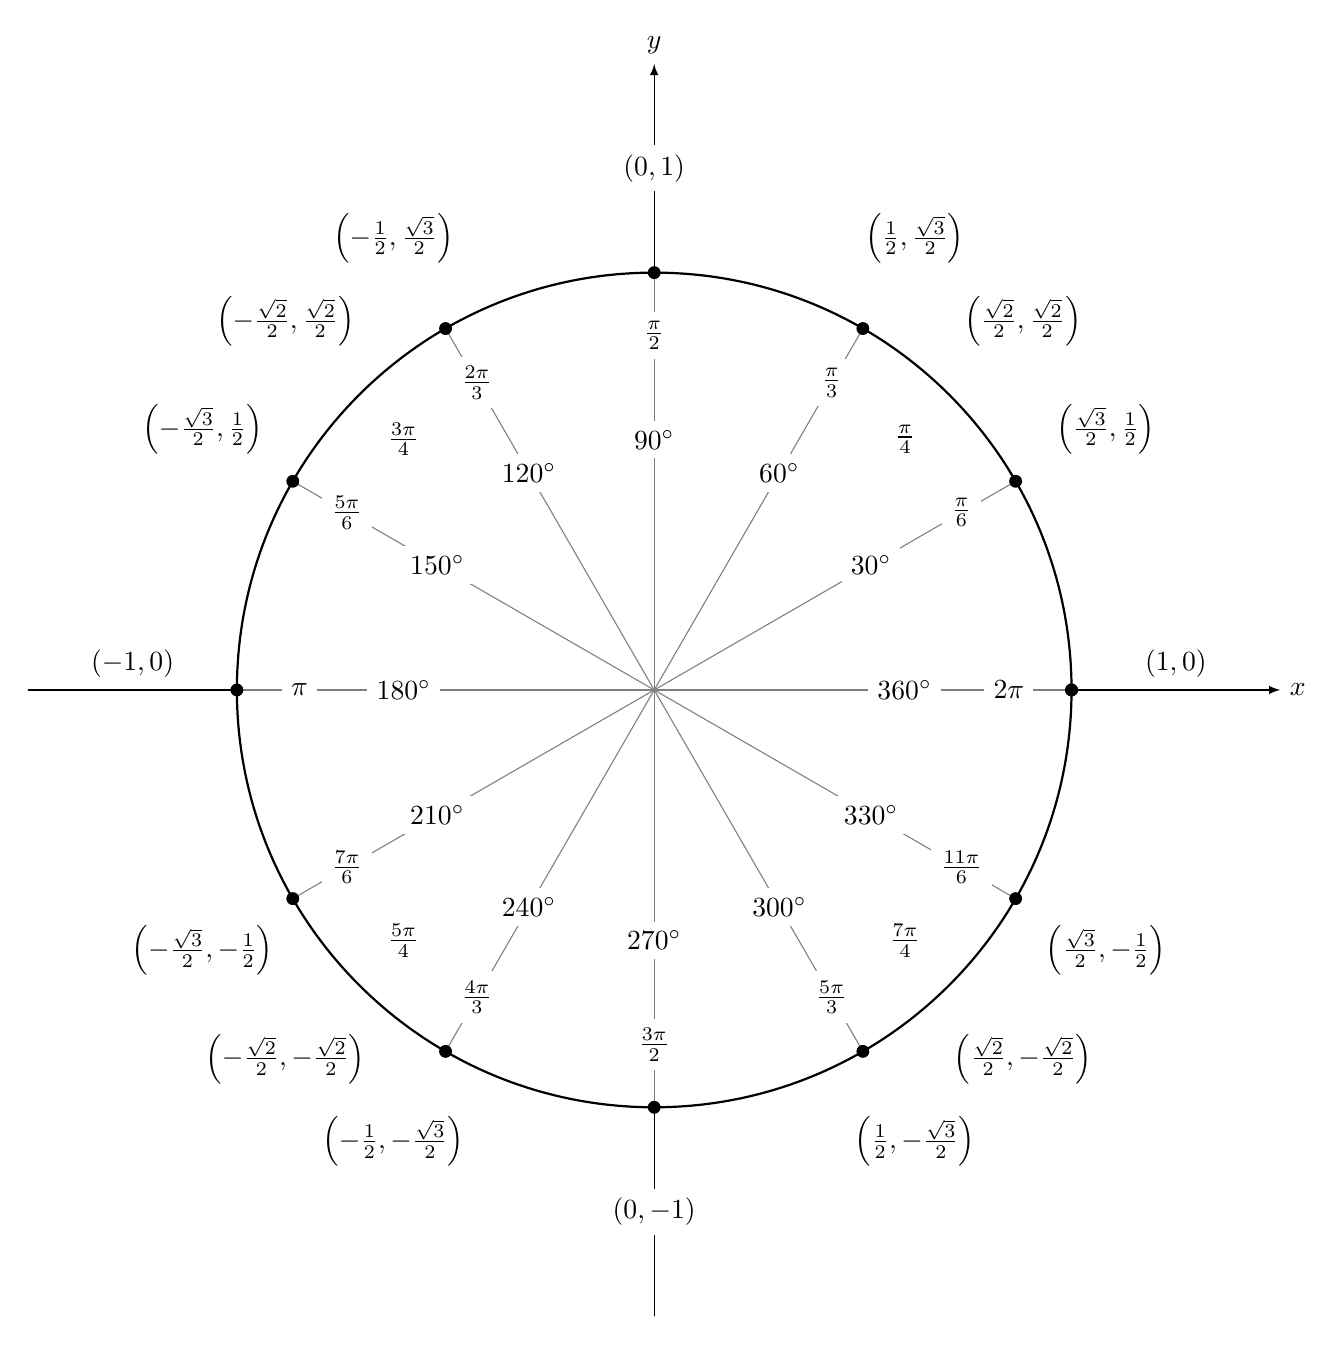
\begin{tikzpicture}[scale=5.3,cap=round,>=latex]
        % draw the coordinates
        \draw[->] (-1.5cm,0cm) -- (1.5cm,0cm) node[right,fill=white] {$x$};
        \draw[->] (0cm,-1.5cm) -- (0cm,1.5cm) node[above,fill=white] {$y$};

        % draw the unit circle
        \draw[thick] (0cm,0cm) circle(1cm);

        \foreach \x in {0,30,...,360} {
                % lines from center to point
                \draw[gray] (0cm,0cm) -- (\x:1cm);
                % dots at each point
                \filldraw[black] (\x:1cm) circle(0.4pt);
                % draw each angle in degrees
                \draw (\x:0.6cm) node[fill=white] {$\x^\circ$};
        }

        % draw each angle in radians
        \foreach \x/\xtext in {
            30/\frac{\pi}{6},
            45/\frac{\pi}{4},
            60/\frac{\pi}{3},
            90/\frac{\pi}{2},
            120/\frac{2\pi}{3},
            135/\frac{3\pi}{4},
            150/\frac{5\pi}{6},
            180/\pi,
            210/\frac{7\pi}{6},
            225/\frac{5\pi}{4},
            240/\frac{4\pi}{3},
            270/\frac{3\pi}{2},
            300/\frac{5\pi}{3},
            315/\frac{7\pi}{4},
            330/\frac{11\pi}{6},
            360/2\pi}
                \draw (\x:0.85cm) node[fill=white] {$\xtext$};

        \foreach \x/\xtext/\y in {
            % the coordinates for the first quadrant
            30/\frac{\sqrt{3}}{2}/\frac{1}{2},
            45/\frac{\sqrt{2}}{2}/\frac{\sqrt{2}}{2},
            60/\frac{1}{2}/\frac{\sqrt{3}}{2},
            % the coordinates for the second quadrant
            150/-\frac{\sqrt{3}}{2}/\frac{1}{2},
            135/-\frac{\sqrt{2}}{2}/\frac{\sqrt{2}}{2},
            120/-\frac{1}{2}/\frac{\sqrt{3}}{2},
            % the coordinates for the third quadrant
            210/-\frac{\sqrt{3}}{2}/-\frac{1}{2},
            225/-\frac{\sqrt{2}}{2}/-\frac{\sqrt{2}}{2},
            240/-\frac{1}{2}/-\frac{\sqrt{3}}{2},
            % the coordinates for the fourth quadrant
            330/\frac{\sqrt{3}}{2}/-\frac{1}{2},
            315/\frac{\sqrt{2}}{2}/-\frac{\sqrt{2}}{2},
            300/\frac{1}{2}/-\frac{\sqrt{3}}{2}}
                \draw (\x:1.25cm) node[fill=white] {$\left(\xtext,\y\right)$};

        % draw the horizontal and vertical coordinates
        % the placement is better this way
        \draw (-1.25cm,0cm) node[above=1pt] {$(-1,0)$}
              (1.25cm,0cm)  node[above=1pt] {$(1,0)$}
              (0cm,-1.25cm) node[fill=white] {$(0,-1)$}
              (0cm,1.25cm)  node[fill=white] {$(0,1)$};
\end{tikzpicture}

\newpage

\textbf{Sats:}\par
\begin{align*}
  &\quad 360^\circ = 2\pi rad \\
  &\quad v_{g} = v_{r} * \frac{180^\circ}{\pi} \\
  &\quad v_{r} = v_{g} * \frac{\pi}{180^\circ} \\
\end{align*}

\textbf{Sats:}\par
\begin{align*}
  &\quad -1 \leq \sin{t} \leq 1 \\
  &\quad -1 \leq \cos{t} \leq 1 \\
\end{align*}

\textbf{Sats:}\par
\begin{align*}
  &\quad \cos{(-t)} = \cos{(t)} \\
  &\quad \sin{(-t)} = -\sin{(t)} \\
  &\quad \tan{(-t)} = \frac{\sin{(-t)}}{\cos{(-t)}} = \frac{-\sin{(t)}}{\cos{(t)}} \\
\end{align*}

\textbf{Additionsformlerna:}\par
\begin{align*}
  &\quad \sin{(\alpha + \beta)} = \sin{(\alpha)}\cos{(\beta)} + \sin{(\beta)}\cos{(\alpha)} \\
  &\quad \sin{(\alpha - \beta)} = \sin{(\alpha)}\cos{(\beta)} - \sin{(\beta)}\cos{(\alpha)} \\
  &\quad \cos{(\alpha + \beta)} = \cos{(\alpha)}\cos{(\beta)} - \sin{(\beta)}\sin{(\alpha)} \\
  &\quad \cos{(\alpha - \beta)} = \cos{(\alpha)}\cos{(\beta)} + \sin{(\beta)}\sin{(\alpha)} \\ 
\end{align*}

\textbf{Trigonometriska ettan:}\par
\begin{align*}
  &\quad (\sin{t})^{2} + (\cos{t})^{2} = 1 \\
  &\quad \sin^{2}{t} + \cos^{2}{t} = 1 \\ 
\end{align*}


\subsection{Tillvägagångs sätt}
\begin{align*}
  \begin{aligned} \cos \frac { \pi } { 12 } & = \cos \left( \frac { \pi } { 3 } - \frac { \pi } { 4 } \right) = \cos \frac { \pi } { 3 } \cos \frac { \pi } { 4 } + \sin \frac { \pi } { 3 } \sin \frac { \pi } { 4 } \\ & = \left( \frac { 1 } { 2 } \right) \left( \frac { 1 } { \sqrt { 2 } } \right) + \left( \frac { \sqrt { 3 } } { 2 } \right) \left( \frac { 1 } { \sqrt { 2 } } \right) = \frac { 1 + \sqrt { 3 } } { 2 \sqrt { 2 } } \end{aligned}
\end{align*}

\end{multicols} \newpage
\chapter{Program Design and Data Structures}

\newpage


\begin{multicols}{2}
\section{Coding convension}
\noindent\textbf{VARIANT} \newline
A (recursive) function terminates if it has a variant.
The variant need to follow all of the flowing rules

\begin{itemize}
\item Needs to decrease every recursive call
\item All ways positive
\end{itemize} 

\noindent\textbf{Side effects} \newline
All IO functions have side effects in order to separate pure Haskell function with impure functions
that changes the state with is commonly the case with imperative and object oriented programming.
Every IO function has a side effects.

\noindent\textbf{INVARIANT} \newline
A data types invariant is what value are allowed for the data type to work. Similar to preconditions for
a function. An example is integer data type that can only use positive integers therefor the
invariant is positive integers.



\section{Design approach}
\begin{itemize}
\item top-down design (Cheating): Is to break down a complex system in to subsystems to solve the problem.
  Most often is to write everything by scratch.
\item bottom-up design (Stacking): Is to piece existing system together to create a more complex system.
  little is programmed, most is copied.
\item dodging: Get some code working more quickly, make progress with some part of the system
  and back-paddle to the dodged part later. The reason is to develop insight that will help solve
  the larger problem.
\end{itemize}


\subsection{Process}
\begin{enumerate}
\item  Data Description
\item  Data Examples
\item  Function Description
\item  Function Examples
\item  Function Template
\item  Code
\item  Tests
\item  Review and Refactor
\end{enumerate}

\noindent\textbf{Programming to an Interface}
More dynamic, can change models, less code to write and a layer of abstraction. ADT 


\section{Recursion}
\subsection{Recursion types}
\begin{enumerate}
\item Simple recursion: There is at most one recursive call (in each branch)
  and the argument is decremented by one.
\item Complete recursion: Some argument becomes smaller in the recursive call, but not necessarily.
\item Multiple recursion: There are multiple recursive calls (in the same branch).
\item Mutual recursion: Two or more functions are defined in terms of each other.
\item Nested recursion: An argument to a recursive call is computed by a recursive call.
\item Recursion on a generalized problem: Sometimes, no suitable recursion scheme is obvious.
\end{enumerate}


\section{Complexity}
\subsection{Growth}
\begin{enumerate}
\item Big $ \theta $ Notation: estimate of growth in intervals determine by constants
  Definition
  For non-negative functions f and g, $f (n) = \theta (g (n))$ if and only if there
  exist $ n_0 \geq 0 $ and $ c_1 , c_2 > 0 $ such that for all $ n > n_0 $
  $ c_1 \cdot g (n) \leq f (n) \leq c_2 \cdot g (n) $.
  $ \theta (g (n)) $ is the set of all functions $ f(n) $ that are bounded below and above
\item Big $ \Omega $ Notation: estimate of growth Lower bound
\item Big $ O $: Notation: estimate of growth upper bound
\end{enumerate}


\subsubsection{Relation}
$O(g(n)) \cap \omega (g(n)) = \theta (g(n))$


\section{Recurrences}
\noindent\textbf{Example:} \newline
sumList $[]$ = 0 \newline
sumList (x:xs) = x + sumList xs

\begin{enumerate}
\item pattern matching $[]$ takes $t_0$ time
\item pattern matching $(x:xs)$ takes $t_1$ time
\item Adding x with recursive call takes $t_{add}$
\item Then the recursive call takes $T(n-1)$
\end{enumerate}

\[ T(n) =
  \begin{cases}
    t_0                   & \quad \text{if } n = 0 \\
    T(n-1)+t_{add} +t_{1}  & \quad \text{if } n > 0 
  \end{cases}
\]


\subsection{Closed Form}
\noindent\textbf{1. Use the substitution method to obtain a closed form for the following recurrence:}
\begin{align*}
  &\quad  f(0) = 5 \\
  &\quad  f(n) = f(n -1) + n + 2, n> 0 \\
\end{align*}
\textbf{Hint: $1 + 2 + 3 + · · · + n = \frac{n(n+1)}{2}$ — you do not need to prove this fact.}


\subsubsection{Expansion Method}
\begin{flalign*}
  & f(0) = 5 \\
  & f(1) = f(0) +n +2 = n +5 +2 \\
  & f(2) = f(1) +n +2 = 2n +5 +2 +2 \\
  & f(3) = f(2) +n +2 = 3n +5 +2 +2 +2 \\
  & f(n) = +n^2 +5 +n \cdot 2 \\
\end{flalign*}
\end{multicols}
\raggedcolumns

\noindent\textbf{Induction proof}
\begin{align*}
  &\quad  \text{Step1: test with base case sense the base case is predefine for 0 we do } n=1  \\
  &\quad  {f(1)}_{VL} = 1^2 +5 +1 \cdot 2 = 8, \\
  &\quad  {f(1)}_{HL} = f(0) +1 +2 = 5 +3 = 8 \\
  &\quad  {f(1)}_{VL} = {f(1)}_{HL} \\
  &\quad  \\
  &\quad  \text{Step2: assumption for p } f(p) = p^2 +5 +p \cdot 2 \\
  &\quad  {f(p+1)}_{VL} = f(p) +(p+1) +2 = (p^2 +5 +p \cdot 2) +(p+1) +2 = \\
  &\quad  = (p^2 +(p+1)) +5 +(p+1) \cdot 2 = (p^2+2p+1) +5 +(p+1) \cdot 2 \\
  &\quad  {f(p+1)}_{HL} = (p+1)^2 +5 +(p+1) \cdot 2 = (p^2+2p+1) +5 +(p+1) \cdot 2 \\
  &\quad  {f(p+1)}_{VL} = {f(p+1)}_{HL} \\
  &\quad  \\
  &\quad  \text{Conclusion: according to induction hypothesis the recurrence of the function is equal to } \\
  &\quad  2n + 5 + \frac{n(1+n)}{2} 
\end{align*}


\subsubsection{Substitution Method}
\begin{align*}
  f(n) &\quad = f(n-1) + n + 2  \\
  &\quad = (f(n-2) + (n-1) + 2) +1n +2 \\               &\quad = f(n-2) + (n-1) + n +2 \cdot 2 \\
  &\quad = (f(n-3) + (n-2) + 2) (n-1) + n +2 \cdot 2 \\ &\quad = f(n-3) +(n-2) + (n-1) + n +3 \cdot 2 \\
  &\quad . \\
  &\quad = f(n-k) + (n -(k-1)) + (n -(k-2)) + (n -(k-3)) + \ldots + n +k \cdot 2  \\
  &\quad . \\
  &\quad = f(n-n) + (n -(n-1)) + (n -(n-2)) + (n -(n-3)) + \ldots + n +n \cdot 2 \\
  &\quad = f(0) +1 +2 +3 + \ldots + n +n \cdot 2 = 5 +1 +2 +3 + \ldots + n +n \cdot 2\\
\end{align*}

We can see the following patterns
\begin{align*}
  &\quad 2n + 5 + \displaystyle\sum_{k=1}^{n}(k) = 2n + 5 + \frac{n(1+n)}{2} \\
\end{align*}

\noindent\textbf{Induction proof}
\begin{align*}
  &\text{Step1: test with base case since the base case is predefine for 0 we do } n=1  \\
  {f(1)}_{VL} &= 2 \cdot 1 + 5 + \frac{1(1+1)}{2} = 2 +5 +1 = 8, \\
  {f(1)}_{HL} &= f(0) + 1 +2 = 5 +3 = 8 \\
  {f(1)}_{VL} &= {f(1)}_{HL} \\
  &\\
  &\text{Step2: assumption for p } f(p) = 2p + 5 + \frac{p(1+p)}{2} \\
  {f(p+1)}_{HL} &= f(p) +(p+1) +2 = (2p +5 +\frac{p(1+p)}{2}) + (p+1) + 2 = \\
  &= 2(p+1) +5 +\frac{p(1+p)}{2} +p = 2(p+1) +5 +\frac{2(p+1)+p(1+p)}{2} = \\
  &= 2(p+1) +5 +\frac{p^2 +2p +p +2}{2} = \\
  {f(p+1)}_{HL} &= 2(p+1) + 5 + \frac{(p+1)(p+2)}{2} = 2(p+1) + 5 + \frac{p^2 +2p +p +2}{2}  \\
  {f(p+1)}_{VL} &= {f(p+1)}_{HL} \\
  &\\
  &\text{Conclusion: according to induction hypothesis the recurrence of the function is equal to } \\
  &2n + 5 + \frac{n(1+n)}{2} 
\end{align*}


\newpage
\section{Higher-Order Function}
\subsection{Higher-Order Functions on Lists}
\begin{center}
\begin{tabular}{c}
\begin{lstlisting}[language=Haskell]
map :: (a -> b) -> [a] -> [b]
filter :: (a -> Bool) -> [a] -> [a]
foldl :: (a -> b -> a) -> a -> [b] -> a
foldr :: (a -> b -> b) -> b -> [a] -> b  
\end{lstlisting}
\end{tabular}
\end{center}

\subsubsection{map}
maps a function to each element in list.

\subsubsection{filter}
filters elements with a condision

\begin{center}
\begin{tabular}{c}
\begin{lstlisting}[language=Haskell]
filter :: (a -> Bool) -> [a] -> [a]
filter (<6) [6,3,0,1,8,5,9,3] == [3,0,1,5,3]
\end{lstlisting}
\end{tabular}
\end{center}

\subsubsection{foldl}
foldl recurses over a list “from the left,” i.e., it initially applies the
given operation to the first list element and the given start value.
starts from the left (first element) and apply the function to with each element.
Similar to an accumulator. No one uses it since it is some what useless.

\begin{center}
\begin{tabular}{c}
\begin{lstlisting}[language=Haskell]
foldl :: (a -> b -> a) -> a -> [b] -> a
foldl (*) 1 [1,2,3,4] == 24
\end{lstlisting}
\end{tabular}
\end{center}


\subsubsection{foldr}
foldr recurses over a list “from the right,” i.e., it initially applies the
given operation to the last list element and the given start value.
starts from the right (last element) and apply the function to with each element.
Similar to an accumulator.

\begin{center}
\begin{tabular}{c}
\begin{lstlisting}[language=Haskell]
foldr :: (a -> b -> b) -> b -> [a] -> b
foldr (*) 1 [1,2,3,4] == 24
\end{lstlisting}
\end{tabular}
\end{center}


\section{Data types}
%To prevent making simple mistakes by forsing spesific types.

\subsection{Basic}
\begin{center}
\begin{tabular}{c}
\begin{lstlisting}[language=Haskell]
String :: ['char'] --list of charecters
List :: []         --undefine element types and elements
Tuple :: ()        --Predefine elements
Char :: ''         --single carecter
Int :: 1           --Hole number with define size 
Integear :: 1      --Hole number with undefine size
Float :: 1.1       --Real number with double-precision  
Double :: 1.1      --Real number with single-precision 
\end{lstlisting}
\end{tabular}
\end{center}


\subsection{Maybe Type}
If the return is maybe ``nothing'' then the ``Maybe type'' is used, since it dose not have to return
the a specific value. It is not polymorphic since you have to specify the type, however
``Just'' is at of it self polymorphic function. If a operation that requires a specific type one needs to
remove ``Just'', for instance by a let function.


\subsection{New types and enumeration types}
New types: One create more relevant names and format of existing enumeration types.
Overload is a problem with the use of the same operations that can not be used for the same data types.
One needs to create new operations if it is not from the same type class.

Enumeration types: Instead of new types \emph{type} enumeration types uses the operation call \emph{data}.
The difference is that enumeration types is independent from existing types therefor
one becomes more flexible and precise.

\textbf{example}
\begin{center}
\begin{tabular}{c}
\begin{lstlisting}[language=Haskell]
data newTypeOfDataDerection = North | South | East | West
   deriving (Show)  -- inorder to print

:t North 
North :: newTypeOfDataDerection 

-- We can use new types in pattern matching 
oposit :: newTypeOfDataDerection -> newTypeOfDataDerection 
oposit North = South
\end{lstlisting}
\end{tabular}
\end{center}


\subsubsection{Type classes}
A type class is a set of types that support certain related operations.
No function is applied by default to the new type, therefor
you can write ``deriving'' the following functions are good to have

\textbf{type classes to deriving for new data types}
\begin{center}
\begin{tabular}{c}
\begin{lstlisting}[language=Haskell]
  deriving (Show)  -- in order to print in ghci and print normal
  deriving (Eq)  -- To test equality
  deriving (Ord)  -- the first one has the smallest value, order matter for comparison
\end{lstlisting}
\end{tabular}
\end{center}

\textbf{New type classes}
\begin{center}
\begin{tabular}{c}
\begin{lstlisting}[language=Haskell]
class Eq a where
   (==) :: a -> a -> Bool
\end{lstlisting}
\end{tabular}
\end{center}

\textbf{New type classes Instances}
\begin{center}
\begin{tabular}{c}
\begin{lstlisting}[language=Haskell]
instance Eq Colour where
  (==) = eqColour
\end{lstlisting}
\end{tabular}
\end{center}

\begin{figure}[H]
    \centering
    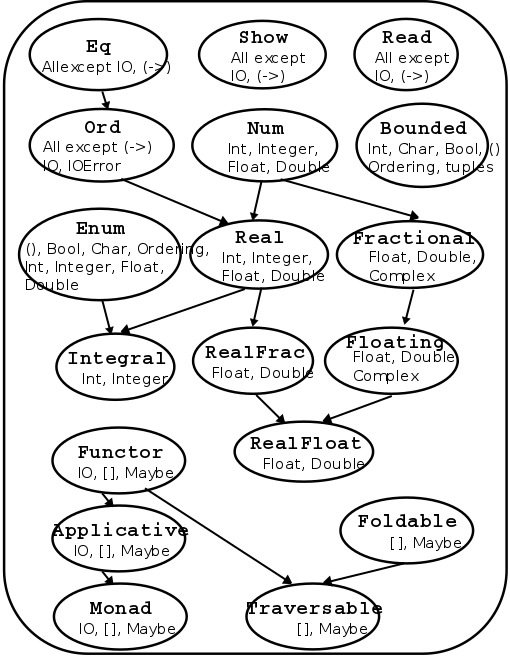
\includegraphics[width=15cm, height=15cm]{image/type-class.png} 
    \caption{Type class \cite{haskell}}
    \label{Type-class}
\end{figure}


\subsection{Inductive Data Types}
Uses a base case then the inductive step as cases of. Multiple arguments. Type constructure

\begin{center}
\begin{tabular}{c}
\begin{lstlisting}[language=Haskell]
data AExp = Atom Int
   | Plus AExp AExp
   | Times AExp AExp

eval (Atom i)    = i
eval (Plus a b)  = eval a + eval b
eval (Times a b) = eval a * eval b
\end{lstlisting}
\end{tabular}
\end{center}

\newpage

\subsection{Trees}
\noindent\textbf{Terminology}
\begin{enumerate}
\item Search tree: All nodes on the left side is less then the parent and opposite on the right side    
\item Out-degree: is how many children it has. Binary trees has out-degree $0-2$
\item root Node: is a parent to any number of children at the top of the hierarchy
\item sub Node: is a parent to any number of children
\item Leaf: is a nod that has no children
\item Node: every element
\item Height: most steps from the root node to a leaf  
\end{enumerate}

\noindent\textbf{Representation}
% https://www.geeksforgeeks.org/tree-traversals-inorder-preorder-and-postorder/
\begin{enumerate}
\item Inorder: (Left, Root, Right)
\item Pre-order: (Root, Left, Right)
\item Post-order: (Left, Right, Root)
\end{enumerate}

\begin{center}
\begin{tabular}{c}
\begin{lstlisting}[language=Haskell]
data FBTree a = Leaf a
   | Node (FBTree a) a (FBTree a)
   deriving (Show)
   
Node (Leaf 1) 5 (Leaf 21)
rootValue :: FBTree a -> a
rootValue (Node _ a _) = a
rootValue (Node x) = x

height :: FBTree a -> Int
height (Leaf _) = 0
height (Node b a c) = 1 + max (height b) (height c)
\end{lstlisting}
\end{tabular}
\end{center}


\newpage
\begin{multicols}{2}
\subsubsection{Binary tree}
\begin{itemize}
  \item Insertion: $O(1)$  ($O(h)$ if search tree)
  \item Delition: $O(n)$   ($O(h)$ if search tree)
  \item Search: $O(n)$  ($O(h)$ if search tree)
  \item Height: $O(n)$ (n nodes)
\end{itemize}

\begin{enumerate}
\item  Full binary tree: has node out-degree either 2 or 0
  worst-case complexity of $O(\log{n})$.
\item  Binary tree: each node has up to an out-degree of 2
\end{enumerate}

\subsubsection{Binary search tree}
\begin{itemize}
  \item Insertion: $O(h)$  ($O(n)$ if search tree)
  \item Delition: $O(h)$
  \item Search: $O(n)$
  \item Height: $O(n)$ (n nodes)
\end{itemize}


\subsubsection{Red and black trees}
\begin{itemize}
  \item Insertion: $O(\log{n})$ % (couldent i be O(n))
  \item Deletion: $O(\log{n})$
  \item Search: $O(\log{n})$ % (couldent i be O(n)), wrong is for BHTree
  \item Element: $O(2^r)$  (rank r) % look it up not shore
  \item Height: $O(2\cdot\log_{2}(n+1))$ (n nodes)
\end{itemize}

Better then a normal binary tree since it balance the tree,
therefor it becomes smaller and more efficient to search in.
One should use red and black tree when there is a large number of nodes, say 50.

Definition: A red-black tree is a binary search tree where every node is
colored either red or black, with the following balancing invariants: 

\begin{enumerate}
\item  No red node has a red parent.
\item  Every path from the root to an empty subtree contains the same.
\item  A red-black tree with n nodes has height at most $2\cdot\log{2}(n+1)$.
\item  there are 4 cases to rebalance (1;4) is similar so is (2;3).
\end{enumerate}

\noindent\textbf{Algorithm}
\begin{enumerate}
\item  Perform a standard binary-search-tree insertion.
\item  Color the new node red.
\item  Rebalance the tree, if there is a red node with a red parent.
\end{enumerate}

\subsubsection{Binomial Trees and heaps}
\begin{itemize}
  \item Insertion: $O(\log{n})$
  \item Search: $O(\log{n})$  (number of trees n)
  \item Element: $2^r$  (rank r, n=1 then r=0)
\end{itemize}

A heap can be used to implement a priority queue, where elements are
added to a pool and assigned a priority. In a min-priority queue,
extraction of an element yields an element with minimum priority.
The smallest node is the root and every child is equal or larger then
its parent.

Binomial Trees is a data structure by linking trees of rank $r-1$ together.
A binomial heap (Vuillemin, 1978) is a list of binomial trees such that
each tree satisfies the min-heap property (hence the root of each tree contains its minimum key);
and the trees have strictly increasing ranks. \newline

\textbf{Terminology}
\begin{enumerate}
\item  Link: putting together two trees.
\item  Merge: putting together two heaps
\item  Binomial Heap: a list (forest!) of Binomial Trees
\item  Binomial Trees have the largest subtree to the left, while Binomial
\end{enumerate}

\textbf{Binomial heaps}
% https://www.youtube.com/watch?v=hbf_h8Ytv04
\begin{enumerate}
\item  Heaps, extracting minimum element in worst case $O(\log{|h|})$
\item  Binomial Trees, The height (here: number of edges on the longest branch) is $r$.
\item  Binomial Trees, There are $2^r$ nodes in the tree.
\item  Binomial Trees, There are $\left(\begin{array}{l}{r}\\{k}\end{array}\right)$ nodes at level k.
  (Hence its name!)
\item  Binomial Trees, The root has r subtrees of ranks $r-1,r-2,\ldots,1,0$.
\item  A binomial heap h has at most $[\lg|h|]+1$ binomial trees.
\item  Inserting a binomial tree into a binomial heap is like addition with base 2.
\item  merging is made with too cases either (case 1) when one is smaller or (case 2) when they are equal
\end{enumerate}

\begin{center}
\begin{tabular}{c}
\begin{lstlisting}[language=Haskell]
  BinoTree = Node Int Int [BinoTree] -- Node rank key (subtrees with decreasing rank)
\end{lstlisting}
\end{tabular}
\end{center}
\end{multicols}
\raggedcolumns


\subsection{Other data types}
\subsubsection{Tables, Stacking and queuing}
\begin{enumerate}
\item  Table: a list of key-value pairs
\item  Stacks: elements accessed in Last-In First-Out (LIFO) order
\item  Queues: elements accessed in First-In First-Out (FIFO) order
\end{enumerate}

\textbf{Table operations}
\begin{center}
\begin{tabular}{c}
\begin{lstlisting}[language=Haskell]
empty :: Table k v
insert :: Eq k => Table k v -> k -> v -> Table k v
exists :: Eq k => Table k v -> k -> Bool
lookup :: Eq k => Table k v -> k -> Maybe v  -- value from key
delete :: Eq k => Table k v -> k -> Table k v
iterate :: Table k v -> (b -> (k, v) -> b) -> b -> b  -- Foldr
keys :: Table k v -> (b -> k -> b) -> b -> b  -- all keys
values :: Table k v -> (b -> v -> b) -> b -> b  -- all values
\end{lstlisting}
\end{tabular}
\end{center}
 

\textbf{Stack operations}
\begin{center}
\begin{tabular}{c}
\begin{lstlisting}[language=Haskell]
-- interface
newtype Stack a = StackImpl [a] -- opaque!

empty :: Stack a
isEmpty :: Stack a -> Bool
push :: a -> Stack a -> Stack a  -- insert
top :: Stack a -> a   -- the first value
pop :: Stack a -> (a,Stack a)  -- take out
\end{lstlisting}
\end{tabular}
\end{center}
 

\textbf{Queue operations}
\begin{center}
\begin{tabular}{c}
\begin{lstlisting}[language=Haskell]
-- interface
newtype Queue a = Q [a] -- opaque

empty :: Queue a  
isEmpty :: Queue a -> Bool
head :: Queue a -> a 
enqueue :: Queue a -> a -> Queue a  -- take out element
dequeue :: Queue a -> Queue a  -- insert element
toList :: Queue a -> [a] 
\end{lstlisting}
\end{tabular}
\end{center}
 
\newpage
\begin{multicols}{2}
\subsubsection{Hashtables}
\begin{itemize}
\item  Key value lookup (an index) 
\item  Array is only define for small index, hash has no limit on avalible keys.
\item  Typically we have n possible keys from set U for a hashtable (which is an array)
  with m slots, where n $\geq$ m.
\item  since there is infinitely many elements and limited amount of key there will be element with
  the  same key, therefor a coalition is created.
\item  Worst-Case Retrieval: time complexity of retrieving a element.
\item  Load Factor: How much data is in the table $\frac{elements}{slots}$
\item  Rehashing: make the hastable more balanced. 
\end{itemize}

\textbf{Collision Resolution by Chaining}
\begin{itemize}
\item Most commonly used collision resolution
\item Let each array slot (also called a bin) hold a list of elements (called a chain).
\item In other words, When collision then add it to a list in that element
\end{itemize}


\textbf{Collision Resolution by Open Addressing}
\begin{itemize}
\item Start with a table with each element is $\perp$ previously used $\Delta$.  
\item Probing: is a function to insert items in a hastable therefore resolves collations
\item Types of probing: \newline
  Linear probing: $f (i)=i$. \newline
  Quadratic probing: $f (i)=c_2\cdot i^2+c_1\cdot i, \; where \; c_2 \neq{0}$. \newline
  Double hashing: $f (i)=i\cdot h'' (i)$, where $h''$ is another hash function. \newline
\item Inserting with Linear Probing: Insert it to the next avalible key 
\item Deleting with Linear Probing: Ignores  $\perp$ and $\Delta$ idex will change.  
\end{itemize}


\subsection{Graphs}
\subsubsection{Types of graphs}
\begin{itemize}
\item list
\item tree
\item forest
\item Directed Acyclic Graph (DAG)  
\end{itemize}

\subsubsection{Treminolage}
\begin{itemize}
\item Node, vertex (plural: vertices)
\item Edge connects two nodes.
\item Self-loop edge from node to itself
\item Adjacent nodes connected by an edge
\item Degree number of edges from or to a node
\item In-degree number of edges to a node
\item Out-degree number of edges from a node
\end{itemize}

\subsubsection{Representation}
\begin{itemize}
\item \textbf{Adjacency Matrix} — a 2-dimensional array A of $0/1$ values, with $A[i, j]$
  containing the number of edges between nodes i and j (undirected graph),
  or from node i to node j \newline
  $+$ edge existence testing in $\theta(1)$ time \newline
  $-$ finding next outgoing edge in $O|V|$ time \newline 
  $+$ compact representation for dense graphs (when $|E|$ is close to $|V|^2$)
\item \textbf{Adjacency List} — a 1-dimensional array Adj of adjacency lists, with 
  Adj[i] containing a list of the nodes adjacent to node i. \newline
  $+$ finding next outgoing edge in $\theta(1)$ time \newline
  $-$ edge existence testing in $O (|V|)$ time \newline
  $+$ compact representation for sparse graphs (when $|E|$ is much smaller than $|V|^2$)
\item \textbf{Edge List} — a list of tuples, (i, j), for each edge (i, j) (plus a list of the nodes). \newline
  $-$ edge existence test in $\theta(|E|)$. \newline
  $-$ finding next outgoing edge in $O (|E|)$ (unless appropriately sorted). \newline
  $+$ compact representation for sparse graphs (when $|E|$ is much smaller than $|V|^2$)
\end{itemize}


\subsubsection{topological sort}
A topological sort is a linear ordering of all the nodes in a directed acyclic. \newline

\noindent\textbf{Algorithm}
\begin{enumerate}
\item Select a node with in-degree 0.
\item Output it.
\item Remove it.
\item Repeat (from 1) until no nodes are left.
\end{enumerate}
Total running time is $\theta(|V|+|E|)$.

\subsubsection{Graph Traversals}
\begin{itemize}
\item Breadth-first search (BFS). Uses a queue for eatch grey node. \newline
  Time complexity: $\theta(|V|+|E|)$  — linear in the size of the graph.
\item Depth-first search (DFS). Uses a stack for eatch (grey) node and has a rest of nodes (white). \newline
  Time complexity: $\theta(|V|+|E|)$  — linear in the size of the graph.
\end{itemize}

\noindent\textbf{Breadth-First Search: Algorithm} \newline
Input: Some node A.
\begin{enumerate}
\item Paint A gray. Paint other nodes white. Add A to an initially empty FIFO queue of gray nodes.
  All grey nodes is in the queue. It is a queue not a stack so first in first out. 
\item Dequeue head node, X. Paint its undiscovered (white) adjacent nodes gray and enqueue them.
  Paint X black. Repeat until queue is empty. For every black node add it to BFS order (black)
\end{enumerate}

\noindent\textbf{Depth-First Search: Algorithm} \newline
Input: Some node A. \newline

\noindent\textbf{DFS(G)}
\begin{enumerate}
\item Paint all nodes white.
\item For each node v in G: if v is (still) white, DFS-Visit(G,v).
  Each subsequent call to DFS-Visit in line 2 is called a restart.
\end{enumerate}

\noindent\textbf{DFS(G)}
\begin{enumerate}
\item Colour v gray.
\item For each node u adjacent to v: if u is white, DFS-Visit(G,u).
\end{enumerate}


\subsubsection{Strongly-Connected Components}
\begin{itemize}
\item Strongly connected component (SCC): maximal set of nodes
  where there is a path from each node to each other node.
\item Many algorithms first divide a digraph into its SCCs, then process
  these SCCs separately, and finally combine the sub-solutions.
  (This is not divide \& conquer, since a different algorithm is run on each SCC!)
\item An undirected graph can be decomposed into its connected
\end{itemize}

\begin{enumerate}
\item Enumerate the nodes of G in DFS finish order, starting from any node
\item Compute the transpose G T (that is, reverse all edges)
\item Make a DFS in G T, considering nodes in reverse finish order from
  original DFS
\item Each tree in this depth-first forest is a strongly connected component
\end{enumerate}
\end{multicols}


\section{Important syntax}
\subsection{Let}
\begin{center}
\begin{tabular}{c}
\begin{lstlisting}[language=Haskell]
  let x = 1 in x * 2 == 2
  case x of
  1 -> "Hello"
  2 -> "H"
  3 -> "Hel"

  input: 3 == "Hel"
  
  # other examples
  let f x y = x + 3 >= y + 3.1 in f 1 1 == False

  f x = let g z = z+1 in g (g x)
  f 1 == 3
  
\end{lstlisting}
\end{tabular}
\end{center}
 
\begin{center}
\begin{tabular}{c}
\begin{lstlisting}[language=Haskell]
:t div
div :: Integral a => a -> a -> a
  
:t (/)
(/) :: Fractional a => a -> a -> a
\end{lstlisting}
\end{tabular}
\end{center}
 

\subsection{IO}
\textbf{monads}
Is used to return an IO and uses a operation \emph(>>=) that replaces \emph{do-notation}
\begin{center}
\begin{tabular}{c}
\begin{lstlisting}[language=Haskell]
class Monad m where
  (>>=) :: m a -> (a -> m b) -> m b
  return :: a -> m a
\end{lstlisting}
\end{tabular}
\end{center}


\section{Sorting Algorithms}
\begin{enumerate}
\item Insertion Sort: One at a time
\item Bubble Sort: sort in order two a time starting from left and work to the right side.
\item Merge Sort: Divide and Conquer, split into even pies and sort them and then merge/sort again. 
\item Quicksort: Divide and Conquer, takes a pivot to spit smaller and larger.
\end{enumerate}
 \newpage
\chapter{Algebra 1}

\newpage

\begin{multicols}{2}
\section{logik}
\begin{itemize}
\item Utsaga: ett påstående som erhåller antigen värderna sann(S) eller falsk(F) vilket ge en stluten utsaga
eller ej ett sannings värde vilket kallas för öpna utsagor
\item Kombinerade utsagor:
\item Kunjuktion utsagor: består av två utsagor som vi kallar $A$ och $B$
\item and: $\land  (A \land B)$
\item Dissjuntion utsagor: består av två utsagor som vi kallar A eller B
\item or: $\lor  (A \lor B)$
\item icke utsaga A (motsatsen): $\neg A$
\item Alla: $\forall$
\item Minst en:  $\exists$
\item $\neg(\forall x : A) \Leftrightarrow \exists x : \neg A$
\item $\neg(\exists x : A) \Leftrightarrow \forall x : \neg A$
\end{itemize}

\textbf{Exempel:}
\begin{align*}
  &\text{Alla reala tal x gäller att } (x+1)^2 = 0 \\
  &\forall x : (x+1)^2 = 0 \\
  &\neg(\forall x : (x+1)^2 = 0) = \exists x : (x+1)^2 \not = 0 \\
  &\neg A \text{: Det finns reala tal x gäller att } (x+1)^2 \not 0 \\
\end{align*}


\subsection{värde tabeller}
\textbf{Kunjuktions värdetabel:}\par
\begin{center}
\begin{tabular}{ |c|c|c| } 
 \hline
 A  & B  & \(A \land B\) \\ 
 S  & S  & S          \\ 
 S  & F  & F          \\  
 F  & S  & F          \\ 
 F  & F  & F          \\ 
 \hline
\end{tabular}
\end{center}

\textbf{Dissjuktions värdetabel:}\par
\begin{center}
\begin{tabular}{ |c|c|c| } 
 \hline
 A  & B  & \(A \lor B\) \\ 
 S  & S  & S          \\ 
 S  & F  & S          \\  
 F  & S  & S          \\ 
 F  & F  & F          \\ 
 \hline
\end{tabular}
\end{center}



\subsection{Implikationer}
\begin{align*}
  &\quad \text{A medför B: } A \Rightarrow B \text{ (implikaiton)} \\
  &\quad \text{A och B medför varandra: } A \Leftrightarrow B \text{ (ekvivalens)} \\
\end{align*}


\textbf{Implication värdetabell:}\par
\begin{center}
\begin{tabular}{ |c|c|c| } 
 \hline
 A  & B  & \(A \Rightarrow B\) \\ 
 S  & S  & S          \\ 
 S  & F  & F          \\  
 F  & S  & S          \\ 
 F  & F  & S          \\ 
 \hline
\end{tabular}
\end{center}

\textbf{Ekvivalens värdetabel:}\par
\begin{center}
\begin{tabular}{ |c|c|c| } 
 \hline
 A  & B  & \(A \Leftrightarrow B\) \\ 
 S  & S  & S          \\ 
 S  & F  & F          \\  
 F  & S  & F          \\ 
 F  & F  & S          \\ 
 \hline
\end{tabular}
\end{center}


\textbf{Exempel1:}
\begin{equation}
  x = \sqrt{6 - x}
\end{equation}

\begin{align*}
  &x = \sqrt{6 - x} \Rightarrow x^2 = 6 - x \Leftrightarrow x^2 + x - 6 = 0 \\
  &\text{pq-formeln: } x = -\frac{1}{2} \pm \sqrt{\frac{1}{4} + \frac{24}{4}} \\
  &\Leftrightarrow (x=-3) \lor (x=2) \\
  &\text{Eftersom det är en implikation år höger och inte} \\
  &\text{ekvivalens så behöver inte rötterna vara sanna } \\
  &\\
  &\text{Testar för falska rötter: } \\
  &2 = \sqrt{6-2} \text{ Sann} \\
  &2 = \sqrt{6-(-3)} \text{ Falsk } 2 \ne \sqrt{6-(-3)} \\
\end{align*}


\textbf{Exempel2:}\par
\begin{equation}
  (x+2)(x+1) = 2x(x+1)
\end{equation}

\begin{align*}
  &(x+2)(x+1) = 2x(x+1) \text{ is not } \\
  &\Rightarrow (x+2) = 2x \text{ (x=0 is not allowed)} \\
  &\text{Insted do ass following: } \\
  &(x+2)(x+1) = 2x(x+1) \\
  &\Leftrightarrow (x+2)(x+1) - 2x(x+1) = 0 \\
  &\Leftrightarrow (x+1)(x+2-2x) = 0 \\
  &\Leftrightarrow (x+1=0)\lor(2-x=0) \\
  &\text{svar ej: x=1 och x=2} \\
  &\text{svar: x=1 eller x=2} \\
  &\text{svar: } x=1 \lor x=2 \\
\end{align*}


\section{Mängder}
\begin{align*}
  &\text{Naturliga tal: } \mathbb{N} = \{0, 1, 2 , 3 ..  \} \\
  &\text{Heltal: }\mathbb{Z} = \{.. -2, 1, 0, 1, 2 ..  \} \\
  &\text{Rationella tal: }\mathbb{Q} = \{ \frac{a}{b} | a,b \in \mathbb{Z}, b \\
  &\text{Irrationella tal: }\mathbb{P} = \frac{\mathbb{R}}{\mathbb{Q}}eller \{ x | x \in \mathbb{R}, x \notin \mathbb{Q} \} \\
  &\text{Reella tal: }\mathbb{R} =  \mathbb{P} \cup \mathbb{Q} \\
\end{align*}

\begin{align*}
  A \cup B &= \{ x:(x \in A) \lor (x \in B)\} \\
  A \cap B &= \{ x:(x \in A) \land (x \in B)\} \\
  A \setminus B &= \{ x:(x \in A) \land (x \notin B)\} \\
  A^{\text{\#}} &= \{ x:(x \in X) \land (x \notin A)\} \\
\end{align*}

\textbf{Exempel:}
\begin{equation*}
  \text{Bevisa: } X \setminus (A \cup B) = (X \setminus A) \land (X \setminus B) 
\end{equation*}

\begin{align*}
  x &\in (X \setminus (A \cup B)) \Rightarrow (x \in X) \land (x \notin (A \cup B)) \\
  &\Rightarrow (x \in X) \land (x \notin A) \land (x \notin B) \\
  &\Rightarrow (x \in X \setminus A) \land (x \in X \setminus B) \\
  &\Rightarrow x \in (X \setminus A) \land (X \setminus B) \\
  &\Rightarrow X \setminus (A \cup B) \subseteq (X \setminus A) \land (X \setminus B)
\end{align*}


\section{Bevis}
\subsection{Induktions bevis}
\begin{itemize}
  \item steg 1: bevisa att det gäller för basfallet.
  \item Steg 2: bevvisar att p => p.
  \begin{itemize}
    \item a. Antar att det stämmer för pp.
    \item b. Vissar att med att stopa in antagandet i pp+1 så blir hl = vl.
  \end{itemize}
\end{itemize}
Tips: Förenkla hl först och sedan vl på klad papper fram och tillbacka. \newline

\textbf{Exempel Recursion:}
\begin{align*}
  &a_1 = 2, a_{n+1} = \frac{7a_n}{7-a_n}, n \in \mathbb{N} \\
  &\text{Vissa med induktion att } a_{n+1} = \frac{14}{7-2n} \\ 
  &\text{Bevis med induktions} \\
  &\text{steg 1: visar att påståendet som vi kallar p } \\
  &\text{gäller för basfallet (n=1)} \\
  &VL_1: a_{1+1}=a_2=\frac{7 \cdot 2}{7-2}=\frac{14}{5}, \\
  &HL_1: a_{1+1}=a_2=\frac{14}{7-2}=\frac{14}{5} \\
  &\\
  &\text{steg 2: visar att } p_m \Rightarrow p_{m+1} \\
  &\text{steg 2a: antar att } p_m \text{ gäller} \\
  &a_{m+1}=\frac{14}{7-2m}\\
  &\text{steg 2b: bevisar attt } p_m \Rightarrow p_{m+1} \\
  &\text{ genom att andvända antagandet} \\
  &VL_{m+1}a_{m+2} 
  = \frac{7a_{m+1}}{7-a_{m+1}} 
  = \frac{7 \frac{14}{7-2m}}{7-\frac{14}{7-2m}} \\
  &= \frac{\frac{7 \cdot14}{7-2m}}{\frac{7(7-2m) - 14}{7-2m}} 
  = \frac{7 \cdot 14}{7(7-2m+2)}
  = \frac{14}{7-2(m+1)} \\
  &HL_{m+1}: \frac{14}{7-2(m+1)} \\
  &\text{Enlight induktionsprincipen är $ p_m $ sann för alla } \\
  &n = 1,2,3 \ldots \text{ VSB}  \\
\end{align*}

\subsection{Motsägelse bevis}
\begin{itemize}
  \item Steg 1: Formulera utsagan och icke utsagan
  \item Steg 2: Hitta en motsägelse med utsagan
\end{itemize}
Tips: Förenka båda led, tänk på teorin vi har, bättre att gå vaga moteveringar en inga alls \newline

\begin{align*}
  &\text{Bevis med motsägelse } \\
  &\text{Antar att motsatsen är sann  } \\
\end{align*}
% Contradiction https://www.youtube.com/watch?v=sRDwsfNDXak
% https://www.youtube.com/watch?v=huGWXh4l1M0


\section{Delbarhet}
$a$ är delbar med $b$, altså kvoten ger ingen rest. 
Vi följand: $a \mid b$


\textbf{Divitions algoritmen:}
\begin{align*}
  &a, b \in \mathbb{Z}  \\
  &a  \geq 0 \land b  \geq  0 \\
  &a \mid b \Rightarrow (q \in \mathbb{Z} : q \geq 0) \land (r \in \mathbb{Z} : 0 \leq r \leq a) \\
  &\text{ Sådant att} \\
  &b = q a + r\\
  &q = \text{ kvoten, } r = \text{ resten} \\
\end{align*}


\subsection{Största Gemensama Delaren (SGD)}
\begin{align*}
  &SGD(a,b) \\
  &a = bq + r \\
  &0 \leq r \leq b \\
\end{align*}

\textbf{Euklides algoritm:}
\begin{align*}
  &SGD(a,b) \\
  &a = bq_1 + r_1 \\
  &b = r_1q_2 + r_2 \\
  &r_1 = r_2q_3 + r_3 \\
  &r_2 = r_3q_4 + r_4 \\
  &. \\
  &. \\
  &. \\
  &r_{k-3} = r_{k-2}q_{k-1} + r_{k} \\
  &r_{k-2} = r_{k-1}q_k + 0 \\
  &SGD(a,b) = r_{k} \\
  &\text{Om } r_{k} = 1 \Rightarrow a \in \text{primtal} \lor b \in \text{primtal} \\
\end{align*}

\textbf{Exempel:}
\begin{align*}
  &\text{Förenkla } \frac{114}{96} \\
  &\\
  &SGD(114,96):    \\
  &114 = 1*96 + 18 \\
  &96  = 5*18 + 6  \\
  &18  = 3*6  + 0  \\
  &\frac{114}{6} = 19 \\
  &\frac{96}{6}  = 16 \\
  &\frac{19}{16} \\
\end{align*}


\textbf{Lemma:}
\begin{align*}
  &a, b \in \mathbb{Z} \\
  &x, y \in \mathbb{Z} \\
  &SGD(a,b) = ax + by  \\
\end{align*}


\textbf{Aritmetiska fundamentalsatsen:}
\begin{align*}
  &a \in \mathbb{Z} \land a \geq 2 \Rightarrow  \\
  &\Rightarrow a \text{ kan endast primtalsfaktoriseras på} \\
  &\text{ETT SÄTT} \\
\end{align*}

\textbf{Lemma 2.7:}
\begin{align*}
  &a \geq 2 \land a \notin \text{ Primatal} \Rightarrow \\
  &\Rightarrow q \in \text{ Primatal} \land q \mid a \land \text{ a går att} \\
  &\text{primtals faktoriera}\\
\end{align*}


\subsection{Primtal}

\textbf{Sats:}
För att bestäma om tal a är ett primtal
\begin{align*}
  &a \geq 1 \land a \in \text{ Primatal} \\
  &\text{om ett tall p finns som dellar a gäller} \\
  &\text{följande} \\
  &2 \leq p \leq \sqrt{a} \leq a \\
\end{align*}


\textbf{Exemple:}
\begin{equation*}
  \text{Bestäm om 211 är ett primtal }
\end{equation*}

\begin{align*}
  &\text{Om 211 är ett primtal så finns det inte} \\
  &\text{en äkta delare a} \\
  &2 \leq a \leq \sqrt{211}  \\
  &\sqrt{211} \approx 16 \\
  &a: \{ \cancel{2}, \cancel{3}, \cancel{5}, \cancel{7}, \cancel{11}, \cancel{13} \} \\
  &\text{a kan inte vara en äktadelare} \\
\end{align*}


\textbf{Euklides algoritm:}
Det finns oändligt många primtal

\textbf{Bevis:}
Motsägelsebevis  
\begin{align*}
  &\text{Antar att det finns ändligt många primtal} \\
  &p_1,p_2,P_3,..,p_n \\
  &M = \displaystyle\prod_{k=1}{n} + 1 \Rightarrow M > p_j, j = 1,2,3,..,n \\
  &\text{Vissar att M är ett primtal} \\
  &1 < b < M \land b \mid M \text{ Där b är minsta äkta delaren} \\
  &\text{av} M \\
  &\Rightarrow M = p_1 * b \Rightarrow p_1 \mid 1 \land p \geq 2
\end{align*}
Detta är falskt eftersom båda utsågorna kan inte vara samtidigt.
Eftersom motsatsen inte fungerar resulterar det i att satsen är sann.


\section{Diofantiska ekvationer} 
\textbf{Sats:}
\begin{align*}
  &ax + by = c \land a,b,c \in \mathbb{Z} \and a \ne 0, b \ne b \\
  &\Rightarrow \\
  &ax + by = c \text{ Där } SGD(a,b) = 1 \\
  &\text{Har den anmäla lösningen:} \\
  &x = C x_0 - n b \land y = C y_0 + n a \\
\end{align*}

\textbf{Exempel:}
En lastbil lastas med 12kg packet och 20kg paket. Totalt väger lasten 296, hur många av varge packet?

\begin{align*}
  &ax + by = C \Leftrightarrow 12x + 20y = 296 \\
  &\text{steg1: Testar om } SGD(a,b) \mid c \\
  &SGD(20,12) = 4 \Rightarrow 4 \mid 269 \\
  &\text{steg2: delar SGD med HL och VL} \\
  &\frac{12x - 20y}{4} = \frac{269}{4} \Leftrightarrow 3x - 5y = 74 \\
  &SGD(5,3): \\
  &5 = 1 \cdot 3 + 2 \\
  &3 = 1 \cdot 2 + 1 \\
  &2 = 2 \cdot 1 + 0 \\
  &\text{steg3: Hjälp ekvation för att hitta} x_0, y_0 \\
  &3x_0 - 5y_0 = 1 \\
  &1 = 3 - 1 * 2 \\
  &1 = 3 - (5 - 3) \\
  &1 = 2 \cdot 3 - 1 \cdot 5 \\
  &x_0 = 2, y_0 = -1 \\
  &\text{steg4: almäna lösningen } x = Cx_0 - bn, y = Cy_0 + an \\
  &x = 74 \cdot 2 - 5n = 148 - 5n \\
  &y = 74 \cdot (-1) + 3n = -74 + 3n \\
  &\text{steg5: hittar godtyckliga lösningar} \\
  &\text{Intervallet som n ligger i för x-termen:} \\
  &n = {\cancel{29}, 28, 27, \ldots }, x = 148 - 5 \cdot 28 = 148 - 140 = 8 \\ 
  &\text{Intervallet som n ligger i för y-termen:} \\
  &n = {\cancel{27}, 28, 29, \ldots }, x = -74 + 3 \cdot 28 = 74 - 84 = 10 \\
  &n = 28, x=8, y=10 \\
  &12 \cdot 8 + 20 \cdot 10 = 296 \\
\end{align*}


\section{Talbaser}
\subsection{konvertera från decimal bass till annan bas}
\begin{align*}
  175_8 &= 1 \cdot 8^2 + 7 \cdot 8^1 + 5 \cdot 8^0 \\
\end{align*}

\subsection{konvertera från annan bas till decimal bas}
\begin{align*}
  1609_{10} &= (3 \cdot 8^3 + 1 \cdot 8^2 + 1 \cdot 8^1 + 1 \cdot 8^0) = 3111_8
\end{align*}

eller så kan man andvända euklides algoritm 
\begin{align*}
  &\text{skriv 517 i talbas 3} \\
  &517 = 172 \cdot 3 + 1 \\
  &172 =  57 \cdot 3 + 1 \\
  & 57 =  20 \cdot 3 + 0 \\
  & 20 =   6 \cdot 3 + 2 \\
  &  6 =   2 \cdot 3 + 0 \\
  &  2 =   0 \cdot 3 + 2 \\
  &\text{Svar: } 517_{tio} = 202011_{tre} \\
\end{align*}


\subsection{Andra exempel}
\textbf{Exempel: Skriv $137_{nio}$  i bass tre}
\begin{align*}
  137_{nio} &= 1 \cdot 9^2 + 3 \cdot 9^1 + 7 \cdot 9^0 \\
  &= 1 \cdot 3^4 + 3 \cdot 3^2 + 7 \cdot 3^0 \\
  &= 1 \cdot 3^4 + 1 \cdot 3^3 + 0 \cdot 3^2 + 2 \cdot 3^1 + 1 \cdot 3^0 \\
  &= 11021_{tre}
\end{align*}


\section{Functioner}
\textbf{Typer av funktioner:}
\begin{itemize}
  \item Injektion: alla element $x$ har olika värden $y$ $f: A \to B, \{{\forall x \in A: x_1 \neq x_2, f(x_1) \neq f(x_2)}\}$
  \item Surjektion: mängd $D$ är definitions mängden  $\{g: C \to D, g(x)=y, (\forall y \in D \land \exists x \in C)\}$
  \item Bijektion: Injektion $\land$ Surjektion
\end{itemize}
 
\textbf{Kareskaprodukten:}
\begin{align*}
  &A \times B = \{ (a,b): a \in A \land b \in B \} \\
  &\text{Låt } A = \{ 1,2,3 \} \land B = \{ x,y,z,w \} \\
  &A \times B : \\
  &\{ (1,x), (1,y), (1,z), (1,w) \\
  &(2,x), (2,y), (2,z), (2,w) \\
  &(3,x), (3,y), (3,z), (3,w) \} \\
\end{align*}

\subsection{Inversen}
En funktions invers kan enda
\begin{align*}
  & f: A \to B \land \text{Bijektiv} \Rightarrow f^{-1}(x) \text{ Finns, där}  \\
  &\text{(1) }  x = f^{-1}(y) \Leftrightarrow y = f(x) \\
  &\text{(2) }  D_{f^-1} = V_f \Leftrightarrow D_f = V_{f^-1} \\
  &\text{(3) }  x = f^{-1}(f(x)), x \in D_f = V_{f^-1} \\ 
  &\text{(3) }  y = f^{-1}(f(y)), y \in D_f = V_{f^-1} \\ 
\end{align*}

\subsection{Relatioiner}
\begin{align*}
  &\text{Relation: } xRy \\
  &\text{Reflexiv: } \forall x \in X: xRx \\
  &\text{Symetrisk: } xRy \Rightarrow yRx, x \in X \land y \in X \\
  &\text{Transitiv: } (xRy) \land (yRz) \Rightarrow xRz, \forall x,y,z \in X  \\
  &\text{Ekvivalnsrelation: Reflexiv och Symetrisk Transitiv} \\
\end{align*}


\section{Summor}
\subsection{Aritmetiska summor}
\begin{equation*}
s _ { n } = a _ { 1 } + a _ { 2 } + a _ { 3 } + \ldots + a _ { n } = \frac { n \left( a _ { 1 } + a _ { n } \right) } { 2 }
\end{equation*}


\subsection{Geometriska summor}
Börjar altid med exponenten 0 och gör om summan så att den passar i följade talföljd:
\begin{equation*}
s _ { n } = a + a k + a k ^ { 2 } + \ldots + a k ^ { n - 1 } = \frac { a \left( k ^ { n } - 1 \right) } { k - 1 }
\end{equation*}


\textbf{Exempel:}
\begin{equation*}
\displaystyle\sum _ { k = n } ^ { 2n } (2^{k} - k)
\end{equation*}

\begin{align*}
  &\text{sätter f = 0 = k -n} \\
  &\displaystyle\sum _ { f = 0 } ^ { n } (2^{f+n} - (f+n)) = 2^{n} * \displaystyle\sum _ { f = 0 } ^ { n } (2^{f}) - \displaystyle\sum _ { f = 0 } ^ { n } (f+n) \\
  &\frac{2^{n} (2^{n+1} -1)}{2-1} - \frac{3n(n+1)}{2} = 2^{2n+1} - 2^{n} - \frac{3n(n+1)}{2}\\
\end{align*}


\section{Kongruensräkning}
\textbf{Räkneregler:}
\begin{align*}
  &a+b \pmod{n} \equiv a \pmod{n} + b \pmod{n} \\
  &a \cdot b \pmod{n} \equiv a \pmod{n} \cdot  b(modn) \\
  &a^b \pmod{n} \equiv (a \pmod{n})^b \\
\end{align*}

\textbf{Exempel: Vilket är det minsta positiva rest som kan erhållas vid division av $19^{18}$ med $17$? }\par
\begin{align*}
  19^{18} &\equiv 2^{18} \pmod{17} \equiv 2^4 \cdot 2^4 \cdot 2^4 \cdot 2^4 \cdot 2^2 \pmod{17} \\
  &\equiv {(-1)}^4 \cdot {(-1)}^4 \cdot {(-1)}^4 \cdot {(-1)}^4 \cdot 2^2 \pmod{17} \\
  &\text{svar: resten blir } 4 \\
\end{align*}


\section{Kardinalitet}
Kardinalitet eller ``mäktighet'' är ett sett att räkna med mängders sorlek och alla
oändliga mängder har samma kardinalitet fast det är en delmängd. Naturliga tall har samma
kardinalitet som reala tal trots att naturliga tal är en del mängd av reala talen

Låt $A$ och $B$ vara mängder. Vi sägger att $A$ och $B$ har samma kardinalitet då det finns en bijektion
$\exists f: A \to B, A \sim B$. Vi säger att $A$ står i relation med $B$ omm $A$ och $B$ har samma kardinalitet $ARB$

\subsection{Uppräkneligamängder}
En mängd $X$ sägs vara upräknerlig omm $X$ har samma kardinalitet som $\mathbb{N}$
$\exists g: \mathbb{N} \to X$ där $g$ är bijektiv.
Exempel på upräknerliga mängder är $\mathbb{N},\; \mathbb{Z},\; \mathbb{Q},\; \{ 1,5,78 \}$
Exempel på ej upräknerliga mängder $\mathbb{R}, (0,1)$


\section{Polynom}
\subsection{Polynom division}
\begin{itemize}
  \item Triviala delare: ej heltals kvot med delaren, har en kostant sådant $\lambda \cdot f, \lambda \notin \mathbb{Z}$
  \item Äkta delare: heltals kvot med delaren $f(x), \exists a \in$ polynom: $a \mid f(x)$
  \item Irreducible: om polynomet endast har triviala delare det finns lösningar heltaslösningar $f(x)=0$
  \item Reducible: om polynomet har äkta delare.
  \item Multiplisitet: vilken grad polynomet har.
\end{itemize}


\textbf{Exempel:}
Man vet att ekvationen $z^4 - 2z^3 - 7z^2 + 26z - 20 = 0$ har roten $z = 2 + i$ Lös ekvationen fullständigt.
$z = 2 + i$ Är en lösning är också konjugatet en lösning enligt faktorsatsen $\overline{\rm z}= a - b i$.
$z = 2 \pm i$ Vilket betyder att följande går att factorisera ut polynomet.
$(z -(2 + i))(z -(2 - i)) = z^2 - 4z + 5$

\textbf{Långdivition (liggande stolen):}\par
\polylongdiv[style=A]{x^{4}-2x^{3}-7x^{2}+26x-20}{x^{2}-4x+5}
$z^2 + 2z - 4 = 0$ Är också en läsning som tilslut ger följande.
$z = -1 \pm \sqrt{5} \land z = 2 \pm i$.
Varge n grads polynom har altid n stycken komplexa lösningar.


\subsection{Faktorsatsen}
\begin{align*} 
  &\quad  f(x) = (x - \alpha)p(x) \\
\end{align*}

\textbf{Exempel, Gemensam root hos två polynom:}
\begin{align*}
  p(x)&=x^4-x^3+x^2+2=0, \\
  g(x)&=x^3+4x^2+4x+3=0 \\
  &\text{Har en Gemensam root} \\
  &\text{Eftersom polynomen har en Gemensam root} \\
  &\text{vet vi att det finns en gemensam} (x-\alpha) \\
  &\\
  f(x)&=(x-\alpha)p_1(x) \\  
  g(x)&=(x-\alpha)p_2(x) \\  
\end{align*}
euklides algoritm:
\begin{align*}
  f(x)&=(x-5)g(x)+17(x^2+x+1) \\
  g(x)&=(\frac{1}{17}(x+3))(17(x^2+x+1)) \\
  &+17(x^2+x+1) + 0 \\
  &\\
  h(x)&=x^2+x+1 \\
  f(x)&= (x-5)(x+3)h(x)+17h(x) \\
  &= h(x)((x-5)(x+3)+17) \\
  &= h(x)(x^2-2x+2) \\
  g(x)&= (x+3)h(x) \\ 
  &\\
  f(x)&=0 \Leftrightarrow (h(x)=0 \lor x^2-2x+2=0) \\
  h(x)&=0 \Rightarrow x=-\frac{1}{2} \pm \frac{\sqrt{3}}{2}i \\
  &x^2+2x+2=0 \Rightarrow x=1 \pm \sqrt{1-2}=1 \pm i \\
\end{align*}

\textbf{Exempel, Heltalslösning med okänd konstant:}
\begin{align*}
  &x^3 + bx^2 - 7x -7 = 0 \text{ har en heltals lösning} \\
  &\text{Eftersom ekvationen har en heltals lösning} \\
  &\text{ vet vi att } \alpha \mid 7\\
  &\text{Kandidaterna är } \{1,-1,7,-7 \} \\
  &I   (x= 1) \;  1 + b\cdot  1 - 7 -7 = 0 \Rightarrow b=13 \in \mathbb{Z} \\
  &II  (x=-1) \; -1 + b\cdot -1 + 7 -7 = 0 \Rightarrow b= 1 \in \mathbb{Z} \\
  &III (x= 7) \;  7 + b\cdot  7 -49 -7 = 0 \Rightarrow b=\_ \notin \mathbb{Z} \\
  &IV  (x=-7) \;  7 + b\cdot -7 +49 -7 = 0 \Rightarrow b=\_ \notin \mathbb{Z} \\
  &\text{svar: b=13, b=1}
\end{align*}

\textbf{Exempel, Rationell root:}
\begin{align*}
  &g(x)= 2x^3 +2x^2 +2x +3 = 0 \text{ har en rationell root} \\
  &\text{Eftersom ploynomet har en rattionel root vet vi att: } \\
  &\frac{p}{q} \; p,q \in \mathbb{Z}, \; SGD(p,q) = 1, \; p \mid 3 \land q \mid 2 \; (a_0) \\
  &\text{Det möjliga delarna är } p=\pm 1,\pm 3, \; q=\pm 1,\pm 2 \\
  &x=-\frac{3}{2} \text{ är den enda av kandidaterna som ger en} \\
  &\text{sann root} \\
  &\text{Vilket vi löser genom polynom divition}
\end{align*}


\textbf{Exempel, Renimaginär root:}
\begin{align*}
  &z^4 + 4z^3 + 8z^2 + 12z +15 = 0 \text{ har en renimachinär root} \\
  &\quad  \text{Eftersom ploynomet har en rentimaghinär root vet vi att } \\
  &z=bi, b \in \mathbb{R}, b \neq 0 \\
  &0= b^4i^4 +4b^3i^3 +8b^2i^2 +12bi +15 \\
  &= b^4 -4b^3i -8b^2 +12bi +15 \\
  &= (b^4-8b^2+15) + (12b-4b^3)i \\
  &=0= b^4-8b^2+15 \\
  &0= 12b-4b^3 = 4b(3-b^2) \Rightarrow b=0, b=\sqrt{3}, b=-\sqrt{3} \\
  &b=0 \text{ är ej en giltig lösning.} \\
  &\text{Enlight faktorsatsen får vi följande} \\
  &p(z)=(z-\sqrt{3}i)(z+\sqrt{3}i)Q(x) = (z^2+3)Q(z) \\
  &\text{Vilket vi löser genom polynom divition}
\end{align*}

\textbf{Exempel, Dubel root:}
\begin{align*}
  &p(t)= t^3 -5t^2 +3t +9 = 0 \text{ har en dubbel root} \\
  &\text{Eftersom ploynomet har en dubbel root vet vi att} \\
  &\text{derivatan ger os en root} p'(t)=0  \\
  &\text{Att räkna ut derivatan gör man genm formeln } \\
  &ax^b \Rightarrow b\cdot ax^{b-1} \\
  &p'(t) = 3t^2 -10t +3 = 0 \Rightarrow t_1=3,t_2=\frac{1}{3} \\
  &\text{ dock är sista en falsk root} \\
  &p(t) = {x-3}^2Q(t) \\ 
  &\text{Vilket vi löser genom polynom divition}
\end{align*}

\textbf{Exempel, SGD polynom:}
\begin{align*}
  &\text{Förenkla } \frac{x^4+x^3+2x-4}{x^4-x^3-2x-4} \\
  &SGD(x^4+x^3+2x-4, x^4-x^3-2x-4):  \\
  &x^4+x^3+2x-4 = 1 \cdot x^4-x^3-2x-4 + (2x^3 +4x) \\
  &x^4-x^3-2x-4 = \frac{x}{2}-\frac{1}{2} \cdot (2x^3 +4x) + (-2x^2-4) \\
  &\text{ med polynom divition} \\
  &2x^3 +4x = -x \cdot (-2x^2-4) +0 \\
  &\text{Med SGD så kan vi ta ett polynom som är hjämt delbart} \\
  &\text{ex:} -2(x^2+x) \\
  &\text{polynom divition: } \frac{x^4+x^3+2x-4}{x^2+x} = x^2+x-2 \\
  &\text{polynom divition: } \frac{x^4-x^3-2x-4}{x^2+x} = x^2-x-2 \\
  &\frac{x^4+x^3+2x-4}{x^4-x^3-2x-4} = \frac{x^2+x-2}{x^2-x-2} \\  
\end{align*}
\end{multicols}
\raggedcolumns

 \newpage
\chapter{Single Variable Calculus}

\newpage

\section{Basic}
\subsection{Mängder}
\begin{align*}
  &\quad \text{Naturliga tal: } \mathbb{N} = \{0, 1, 2 , 3 ..  \} \text{ or } \{1, 2 , 3 ..  \} \\
  &\quad \text{Heltal: }\mathbb{Z} = \{.. -2, 1, 0, 1, 2 ..  \} \\
  &\quad \text{Rationella tal: }\mathbb{Q} = \left\{ \frac{a}{b} \Big| \; a,b \in \mathbb{Z} \right\} \\
  &\quad \text{Irrationella tal: }\mathbb{P} = \frac{\mathbb{R}}{\mathbb{Q}}eller \left\{ x | x \in \mathbb{R}, x \notin \mathbb{Q} \right\} \\
  &\quad \text{Reella tal: }\mathbb{R} =  \mathbb{P} \cup \mathbb{Q} \\
\end{align*}

\begin{align*}
  &\quad A \cup B = \{ x:(x \in A) \lor (x \in B)\} \\
  &\quad A \cap B = \{ x:(x \in A) \land (x \in B)\} \\
  &\quad A \setminus B = \{ x:(x \in A) \land (x \notin B)\} \\
  &\quad A^{\text{\#}} = \{ x:(x \in X) \land (x \notin A)\} \\
\end{align*}


\newpage

\subsection{Intervall}
\begin{align*}
  &\quad \text{Open intervall} = (1,4) \\
  &\quad \text{Closed intervall} = [ \, 1,4 ] \, \\
\end{align*}
\begin{equation}
[ \, a, b ] \, = \{ x | a \leq x \leq b \}
\end{equation}

\begin{equation}
[ \, a, \infty [ \,
\end{equation}
\begin{equation}
] \, -\infty, \infty [ \,
\end{equation}

\textbf{Exempel: Olikheter och intervall}
\begin{equation}
\frac { 2 } { x - 3 } < \frac { 5 } { x }
\end{equation}

\begin{align*}
&\quad \frac{ 2 }{ x - 3 } - \frac{ 5 }{ x } < 0 \\
&\quad \frac{(x) 2 }{x (x - 3)} - \frac{ 5 ( x - 3 )}{ x ( x - 3 ) } < 0 \\
&\quad \frac{ 2 x - 5 x - 15 }{ x ( x - 3 ) } < 0 \\
&\quad \frac{ - 3 x - 15 }{ x ( x - 3 ) } < 0 \\
&\quad \frac{ - 3 ( x - 5 ) }{ x ( x - 3 ) } < 0 \\
&\quad  x \neq 0 , x \neq 3 \\
\end{align*}

Värde tabell:
\begin{center}
\begin{tabular}{ |c|c|c|c|c| } 
 \hline
        & x<0   & 0<x<3 & 3<x<5 & 5<x   \\ 
 x-5    & -     & -     & -     & +     \\ 
 -3     & -     & -     & -     & -     \\  
 x      & -     & +     & +     & +     \\ 
 x-3    & -     & -     & +     & +     \\ 
 hela   & +     & -     & +     & -     \\ 
 \hline
\end{tabular}
\end{center}


\newpage

\subsection{Funktion}
\begin{align*}
  &\quad  f: A \to B \\
  &\quad  \text{A: domain/definitionsmängd, B: Målmängd/kodomängd/värdemängd} \\
  &\quad  \text{Injektion: alla element x har olika värden y } f: A \to B,
  \{{\forall x \in A: x_1 \neq x_2, f(x_1) \neq f(x_2)}\} \\
  &\quad  \text{Surjektion: mängd D är definitions mängden } \{g: C \to D, g(x)=y,
  (\forall y \in D \land \exists x \in C)\} \\
  &\quad  \text{Bijektion: } \text{Injektion} \land \text{Surjektion}  \\
  &\quad  f \circ g = f(g(x)) \\
  &\quad  \text{Begränsad: functionen är inom ett intervall, altså nedåt och uppåt} \\
  &\quad  \text{Begränsat nedåt: functionenn är endast begrensad nedåt} \\
  &\quad  \text{Begränsat uppåt: functionenn är endast begrensad uppåt} \\
  &\quad  \text{Jämn function: altså är den symetrisk, ex: } x^2, \; f(-x)=f(x) \\
  &\quad  \text{Udda function: altså är den spefelvänt symetrisk, ex: } x^3, \; f(-x)=-f(x) \\
  &\quad  \text{Polynom } p(x)=a_nx^n +a_{n-1}x^{n-1}+ \ldots +a_1x +a_0
  = \displaystyle\sum _ { i=0 } ^ { n } (a_i x^{i}) \\
  &\quad  \text{Rationell funktion:} R(x)=\frac{P(x)}{Q(x)} \text{, ex: } x^{-1}
  =\frac{1}{x} \text{ ej polynom men rationell funktion} \\
\end{align*}


\newpage

\subsection{Trigonometri}
\begin{center}
\begin{tabular}{ |c|c|c|c|c|c| } 
 \hline
        & $0$                  & $\frac{\pi}{6}$      & $\frac{\pi}{4}$      & $\frac{\pi}{3}$    & $\frac{\pi}{2}$ \\ 
 $\sin$ & $\frac{\sqrt{0}}{2}$ & $\frac{\sqrt{1}}{2}$ & $\frac{\sqrt{2}}{2}$ & $\frac{\sqrt{3}}{2}$ & $\frac{\sqrt{4}}{2}$ \\ 
 $\cos$ & $\frac{\sqrt{4}}{2}$ & $\frac{\sqrt{3}}{2}$ & $\frac{\sqrt{2}}{2}$ & $\frac{\sqrt{1}}{2}$ & $\frac{\sqrt{0}}{2}$ \\  
 \hline
\end{tabular}
\end{center}


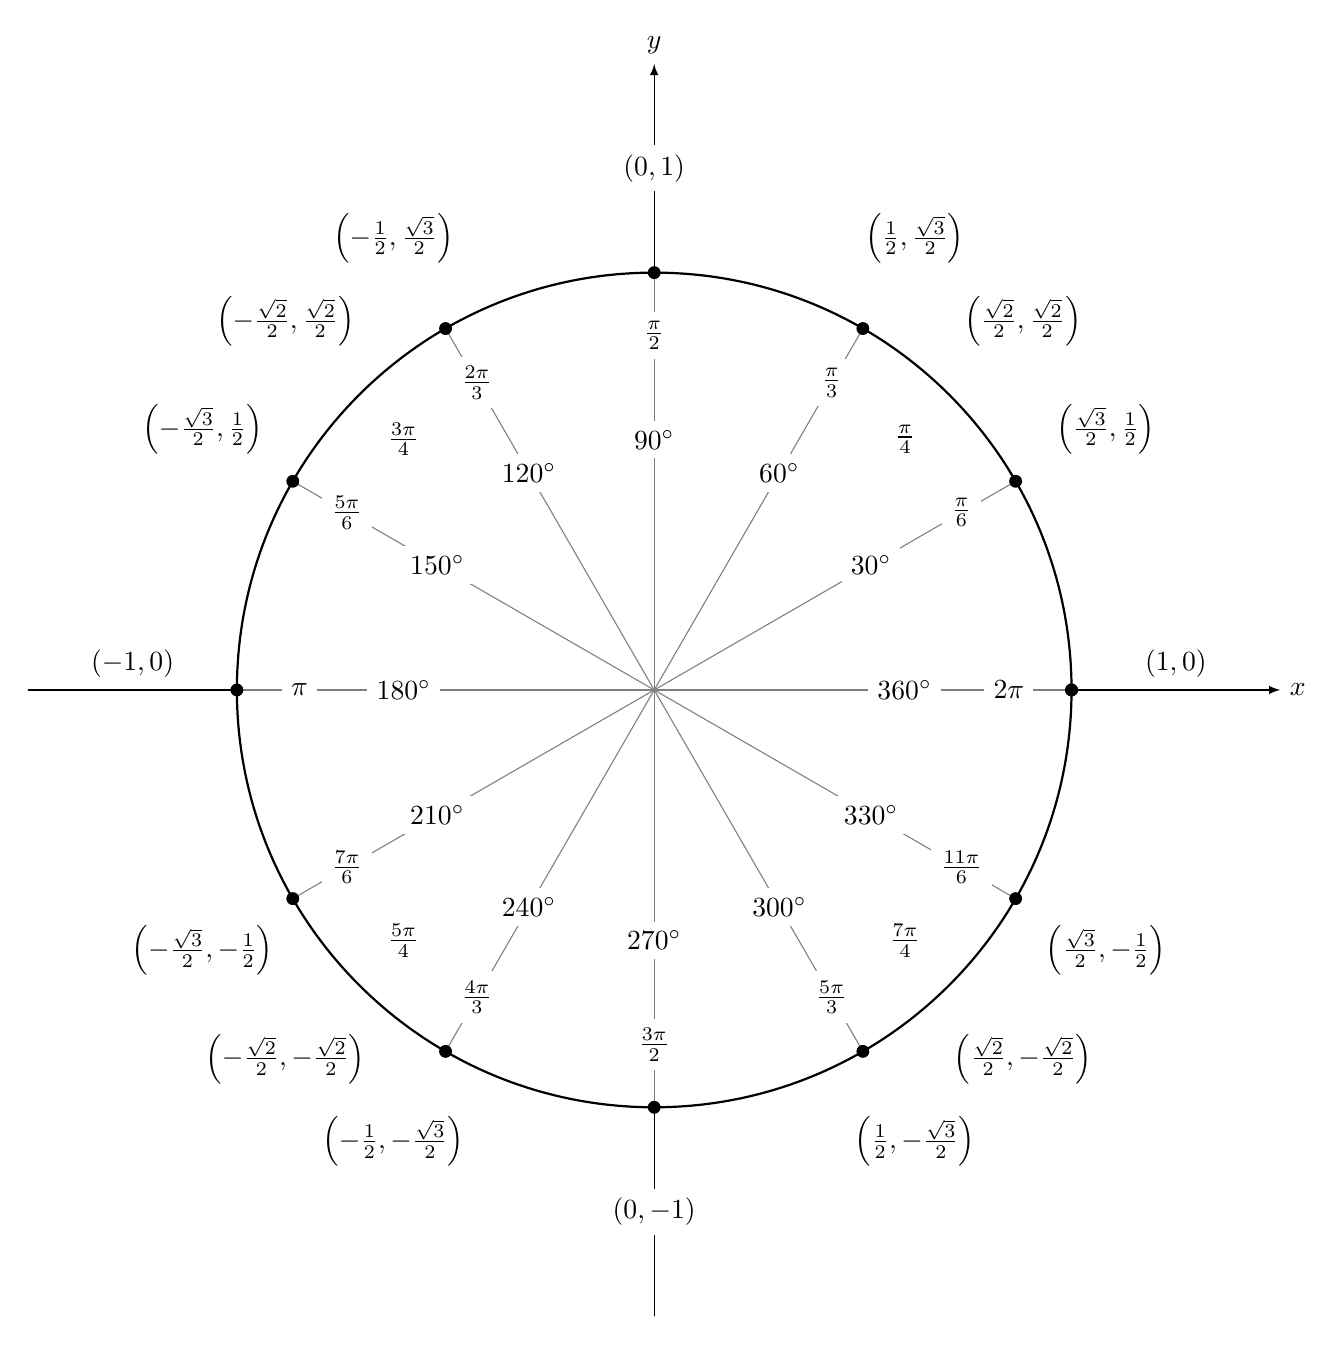
\begin{tikzpicture}[scale=5.3,cap=round,>=latex]
        % draw the coordinates
        \draw[->] (-1.5cm,0cm) -- (1.5cm,0cm) node[right,fill=white] {$x$};
        \draw[->] (0cm,-1.5cm) -- (0cm,1.5cm) node[above,fill=white] {$y$};

        % draw the unit circle
        \draw[thick] (0cm,0cm) circle(1cm);

        \foreach \x in {0,30,...,360} {
                % lines from center to point
                \draw[gray] (0cm,0cm) -- (\x:1cm);
                % dots at each point
                \filldraw[black] (\x:1cm) circle(0.4pt);
                % draw each angle in degrees
                \draw (\x:0.6cm) node[fill=white] {$\x^\circ$};
        }

        % draw each angle in radians
        \foreach \x/\xtext in {
            30/\frac{\pi}{6},
            45/\frac{\pi}{4},
            60/\frac{\pi}{3},
            90/\frac{\pi}{2},
            120/\frac{2\pi}{3},
            135/\frac{3\pi}{4},
            150/\frac{5\pi}{6},
            180/\pi,
            210/\frac{7\pi}{6},
            225/\frac{5\pi}{4},
            240/\frac{4\pi}{3},
            270/\frac{3\pi}{2},
            300/\frac{5\pi}{3},
            315/\frac{7\pi}{4},
            330/\frac{11\pi}{6},
            360/2\pi}
                \draw (\x:0.85cm) node[fill=white] {$\xtext$};

        \foreach \x/\xtext/\y in {
            % the coordinates for the first quadrant
            30/\frac{\sqrt{3}}{2}/\frac{1}{2},
            45/\frac{\sqrt{2}}{2}/\frac{\sqrt{2}}{2},
            60/\frac{1}{2}/\frac{\sqrt{3}}{2},
            % the coordinates for the second quadrant
            150/-\frac{\sqrt{3}}{2}/\frac{1}{2},
            135/-\frac{\sqrt{2}}{2}/\frac{\sqrt{2}}{2},
            120/-\frac{1}{2}/\frac{\sqrt{3}}{2},
            % the coordinates for the third quadrant
            210/-\frac{\sqrt{3}}{2}/-\frac{1}{2},
            225/-\frac{\sqrt{2}}{2}/-\frac{\sqrt{2}}{2},
            240/-\frac{1}{2}/-\frac{\sqrt{3}}{2},
            % the coordinates for the fourth quadrant
            330/\frac{\sqrt{3}}{2}/-\frac{1}{2},
            315/\frac{\sqrt{2}}{2}/-\frac{\sqrt{2}}{2},
            300/\frac{1}{2}/-\frac{\sqrt{3}}{2}}
                \draw (\x:1.25cm) node[fill=white] {$\left(\xtext,\y\right)$};

        % draw the horizontal and vertical coordinates
        % the placement is better this way
        \draw (-1.25cm,0cm) node[above=1pt] {$(-1,0)$}
              (1.25cm,0cm)  node[above=1pt] {$(1,0)$}
              (0cm,-1.25cm) node[fill=white] {$(0,-1)$}
              (0cm,1.25cm)  node[fill=white] {$(0,1)$};
\end{tikzpicture}

\newpage

\textbf{Sats:}\par
\begin{align*}
  &\quad 360^\circ = 2\pi rad \\
  &\quad v_{g} = v_{r} \cdot \frac{180^\circ}{\pi} \\
  &\quad v_{r} = v_{g} \cdot \frac{\pi}{180^\circ} \\
\end{align*}

\textbf{Sats:}\par
\begin{align*}
  &\quad -1 \leq \sin{t} \leq 1 \\
  &\quad -1 \leq \cos{t} \leq 1 \\
\end{align*}

\textbf{Sats:}\par
\begin{align*}
  &\quad \cos{(-t)} = \cos{(t)} \\
  &\quad \sin{(-t)} = -\sin{(t)} \\
  &\quad \tan{(-t)} = \frac{\sin{(-t)}}{\cos{(-t)}} = \frac{-\sin{(t)}}{\cos{(t)}} \\
\end{align*}

\textbf{Additionsformlerna:}\par
\begin{align*}
  &\quad \sin{(\alpha + \beta)} = \sin{(\alpha)}\cos{(\beta)} + \sin{(\beta)}\cos{(\alpha)} \\
  &\quad \sin{(\alpha - \beta)} = \sin{(\alpha)}\cos{(\beta)} - \sin{(\beta)}\cos{(\alpha)} \\
  &\quad \cos{(\alpha + \beta)} = \cos{(\alpha)}\cos{(\beta)} - \sin{(\beta)}\sin{(\alpha)} \\
  &\quad \cos{(\alpha - \beta)} = \cos{(\alpha)}\cos{(\beta)} + \sin{(\beta)}\sin{(\alpha)} \\ 
\end{align*}

\textbf{Trigonometriska ettan:}\par
\begin{align*}
  &\quad (\sin{t})^{2} + (\cos{t})^{2} = 1 \\
  &\quad \sin^{2}{t} + \cos^{2}{t} = 1 \\ 
\end{align*}


\subsection{Exempel: Trigonometri}
\begin{align*}
  \begin{aligned} \cos \frac { \pi } { 12 } & = \cos \left( \frac { \pi } { 3 } - \frac { \pi } { 4 } \right) = \cos \frac { \pi } { 3 } \cos \frac { \pi } { 4 } + \sin \frac { \pi } { 3 } \sin \frac { \pi } { 4 } \\ & = \left( \frac { 1 } { 2 } \right) \left( \frac { 1 } { \sqrt { 2 } } \right) + \left( \frac { \sqrt { 3 } } { 2 } \right) \left( \frac { 1 } { \sqrt { 2 } } \right) = \frac { 1 + \sqrt { 3 } } { 2 \sqrt { 2 } } \end{aligned}
\end{align*}


\newpage


\section{Gränsvärden}
\begin{align*}
  &\quad  \lim_{x\to x_0} f = L \land \lim_{x\to x_0} g = M \Rightarrow \lim_{x\to x_0}(f+g) = L+M  \\
  &\quad  \text{Squeeze therum: } h(x) \leq f(x) \leq g(x), \lim_{x\to x_0} h(x) = \lim_{x\to x_0} g(x_0) = L
  \Rightarrow \lim_{x\to x_0} f(x) = L \\
  &\quad  \lim_{x\to 0} \frac{\sin(x)}{x}=1  \\
  &\quad  \lim_{x\to\infty} \sin(x) \text{ är ej definerad}  \\
\end{align*}


\textbf{Example: Limit för sin}
\begin{align*}
  &\quad  \text{Lös: } \lim_{x\to 0} \frac{\sin(2x^2)}{x^2}  \\
  &\quad  \lim_{x\to 0} \frac{2 \cdot \sin(2x^2)}{2x^2} = 2 \cdot \lim_{x\to 0} \frac{\sin(2x^2)}{2x^2} = 2 \\
\end{align*}

\textbf{Example: 0/0}
\begin{align*}
  &\quad  \text{Lös: } \lim_{x\to 0} \frac{x \cdot \left( \cos(x) + \frac{\sin(x)}{x} \right) }{x+x^2} \\
  &\quad  \lim_{x\to 0} \frac{ x \cdot \left( \cos(x) + \frac{ \sin(x) }{ x } \right) }{x(1+x)} = \frac{1+1}{1} = 2  \\
\end{align*}

\textbf{Example: roten ur i nämnaren}
\begin{align*}
  &\quad  \text{Lös: } \lim_{x\to 0} \frac{x}{\sqrt{x+9}-3}  \\
  &\quad  \lim_{x\to 0} \frac{x(\sqrt{x+9}+3)}{(\sqrt{x+9}-3)(\sqrt{x+9}+3)} =
  \lim_{x\to 0} \frac{x(\sqrt{x+9}+3)}{x+9-9} = \lim_{x\to 0} \sqrt{x+9}+3 = 6   \\
\end{align*}

\textbf{Example: roten ur i nämnaren}
\begin{align*}
  &\quad  \text{Lös: } \lim_{x\to-\infty} \frac{2x-1}{\sqrt{3x^2+x+1}}  \\
  &\quad  \lim_{x\to-\infty} \frac{x(2-\frac{1}{x})}{\sqrt{x^2(3+\frac{1}{x}+\frac{1}{x^2})}} =
  \lim_{x\to-\infty} \frac{x(2-\frac{1}{x})}{x\sqrt{3+\frac{1}{x}+\frac{1}{x^2}}} = \frac{-2}{\sqrt{3}} \\
  &\quad   \\
  &\quad   \\
\end{align*}

\textbf{Example: infinity sin and squeeze}
\begin{align*}
  &\quad  \text{Lös: } \lim_{x\to\infty}\frac{\sin(x)}{x}  \\
  &\quad  |\frac{\sin(x)}{x}| = \frac{|\sin(x)|}{|x|} \leq \frac{1}{|x|} \Rightarrow \text{ squeeze }
  \lim_{x\to\infty}|\frac{\sin(x)}{x}| = 0  \\
  &\quad  \Rightarrow \lim_{x\to\infty}\frac{\sin(x)}{x} = 0  \\
\end{align*}


\subsection{Kontinuitet}
\begin{align*}
  &\quad  \text{En funktion är kontnuelig i punkt } x_0, \; \forall \varepsilon \land \exists \delta: |x-x_0| < \delta \Leftrightarrow |f(x)-f(c_0)|<\varepsilon. \\
  &\quad  \text{Altså så finns det inga hopp i funktionen. Man kan dra penan på grafen utan att släppa} \\
  &\quad  \text{om functionen bestor av flera utryck är funktionen kontenuerlig om alla utrycken är det } \\
\end{align*}


\section{Derivator}
\begin{align*}
  &\quad  \text{Tangent: linjen som har samma lutining i en punkt som functionens derivata} \\
  &\quad  y-f(x_0)=f'(x_0)(x-x_0) \Rightarrow y=ax+b \\ %y-f(x_0)=f'(x_0)(x-x_0)
  &\quad  \text{Samband: } Deriverbar \Rightarrow Kontinuerlig \\
\end{align*}

\textbf{Räkneregler}
\begin{center}
\begin{tabular}{ |c|c| } 
 \hline
 $f$       & $f'$         \\
 \hline
 $c$       & $0$          \\
 $x$       & $1$          \\ 
 $x^n$     & $nx^{n-1}$    \\  
 $a^x$     & $a^x\ln{a}$   \\ 
 $e^{kx}$  & $ke^{x}$       \\
 $\sin{x}$ & $\cos{x}$     \\
 $\cos{x}$ & $-\sin{x}$    \\
 $\tan{x}$ & $\frac{1}{\cos^2{x}}$    \\
 $\ln{x}$  & $\frac{1}{x}$ \\
 \hline
\end{tabular}
\end{center}

\begin{align*}
  &\quad  (f+g)' = f' + g' \\
  &\quad  (cf)'  = cf' \\
  &\quad  (fg)'  = f'g + fg' \text{ Produktregeln} \\
  &\quad  \left( \frac{f}{g} \right)' = \frac{f'g - fg'}{g^2} \text{ Kvotregeln, } g \neq 0 \\
\end{align*}

% derivatans Definetion
% flertal exemplel med squeeze, modifiering(0/0), sin
% tangent

\subsection{Kjedje regeln}
\begin{align*}
  &\quad  \text{Om functionen $f$ är deriverbar i $x$ och funktionen är deriverbar i } g(x) \\
  &\quad  \Rightarrow h(x)=f \circ g = f(g(x)) \text{ deriverbar i } x \\
  &\quad  h'(x)=(f(g(x)))'=f'(g(x))g'(x) \\ 
\end{align*}

\textbf{Example: Kjedje regeln}
\begin{align*}
  &\quad  \text{Lös: } (x^x)'  \\
  &\quad  (x^x)'=\left( e^{x\ln{x}} \right)'=e^{x\ln{x}} \left( \ln{x}+x\frac{1}{x} \right) = e^{x\ln{x}}(1+\ln{x})=x^x(1+\ln{x}) \\
\end{align*}

\newpage

\subsection{L'Hôpital's rule} 
\begin{align*}
  &\quad  f,g:\mathbb{R}\to\mathbb{R} \land \left( \lim_{x \to x_0}\frac{f}{g}
  =\frac{0}{0}\lor ''{\lim_{x\to x_0}\frac{f}{g}=\frac{\pm \infty}{\pm \infty}}'' \right)
  \Rightarrow \lim_{x \to x_0}\frac{f}{g}=\lim_{x \to x_0}\frac{f'}{g'} \\ 
\end{align*}

\textbf{Example: L'Hôpital's rule}
\begin{align*}
  &\quad  \text{Lös: } \lim_{x \to 1}\frac{x^4-6x^3+5x^2}{x^3-8x^2+7x}\\
  &\quad  \lim_{x \to 1}\frac{x^4-6x^3+5x^2}{x^3-8x^2+7x} = '' \; \frac{0}{0} \; '' \\
  &\quad  \text{L'Hôpital's rule} \Rightarrow \lim_{x \to 1}\frac{4x^3-18x^2+10x}{3x^2-16x+7} \\
  &\quad  = \frac{-4}{-6} = \frac{2}{3} \\
\end{align*}


\subsection{Medelvärdessatsen} 
\begin{align*}
  &\quad  \text{Anta att $f$ är kontinuerlig på $[a,b]$ och deriverbar på $(a,b)$}
  \Rightarrow \exists c \in (a,b) \\
  &\quad  \text{så att } \frac{f(b)-f(a)}{b-a}= f'(c)
\end{align*}

\textbf{Example: Medelvärdessatsen}
\begin{align*}
  &\quad  \text{Bevisa att för varge $a>b$ gäller följande} |\cos{a}-\cos{b}| \leq |a-b| \\
  &\quad  f(x)=\cos{x} \text{ är kont och deriverbar i } \mathbb{R} \land [ \, a,b ] \, \\
  &\quad  \text{MVS }\Rightarrow \exists c \in (a,b):f'(c)=\frac{f(b)-(a)}{b-a}=
  \frac{\cos(b)-\cos(a)}{b-a}=-\sin(c) \\
  &\quad  \Rightarrow |\frac{\cos(b)-\cos(a)}{b-a}|=|-\sin(c)| \Rightarrow
  \frac{|\cos(b)-\cos(a)|}{|b-a|}=|-\sin(c)| \leq 1 \\
  &\quad  \frac{|\cos(b)-\cos(a)|}{|b-a|} \leq 1 \Rightarrow |\cos(b)-\cos(a)| \leq |a-b|
\end{align*}


\subsection{Rolle} 
\begin{align*}
  &\quad  \text{Anta att $f$ är kontinuerlig på $[a,b]$ och deriverbar på $(a,b)$. Om } f(a)=f(b) \Rightarrow
  \exists c \in (a,b):f'(c)=0 \\
\end{align*}


\newpage


\subsection{växande funktioner}
\begin{align*}
  &\quad  \text{växande: }          x_1<x_2 \Rightarrow f(x_1) \leq f(x_2) \\
  &\quad  \text{strängt växande: }   x_1<x_2 \Rightarrow f(x_1) < f(x_2)    \\
  &\quad  \text{avtagande: }        x_1<x_2 \Rightarrow f(x_1) \geq f(x_2) \\
  &\quad  \text{stänkt avtagande: } x_1<x_2 \Rightarrow f(x_1) > f(x_2)    \\
\end{align*}


\subsection{Högreordnings devivator}
\begin{align*}
  &\quad  \text{andragrads derivator: }  (f')' = f''  =\frac{d^2f}{dx^2} \\
  &\quad  \text{tredjegrads derivator: } (f'')'= f''' =\frac{d^3f}{dx^3} \\
  &\quad  \text{ntegrads derivator: }    f^{(n)}= f^{n}=\frac{d^{n}f}{dx^{n}} \\
\end{align*}


\subsection{Impericit derivering}
\begin{align*}
  &\quad  \text{deriverar båda sidorna om modifierat } \\
\end{align*}

\textbf{Example: Impericit derivering}
\begin{align*}
  &\quad  \text{Bestäm tangenten till } x^3+y^3=6xy \; i \; (3,3) \\
  &\quad  (3^3+3^3=6\cdot3\cdot3) \text{ -sant} \\
  &\quad  y-y_0=f'(x_0)(x-x_0) \Rightarrow y-3=f'(3)(x-3) \\
  &\quad  \text{Implicit derivering: } 3x^2+3y^2y'=6y+6xy' \\
  &\quad  \Rightarrow 3x^2y'-6xy'=6y-6x^2
  \Rightarrow y'(3x^2-6x)=6y-3x^2
  \Rightarrow y'=\frac{6y-3x^2}{3x^2-6x} \\
  &\quad \Rightarrow y'(3)=\frac{63-3\cdot3^2}{3\cdot3^2-6\cdot3}=-1 \\
  &\quad \Rightarrow y-3=-(x-3) \Rightarrow x+y=6 \lor y=-x+6 \\
\end{align*}


\subsection{invers funktioner} 
\begin{align*}
  &\quad  f: A \to B \land Bijektiv \Rightarrow f^{-1}(x) \text{ Finns, där}  \\
  &\quad \text{(1) }  x = f^{-1}(y) \Leftrightarrow y = f(x) \\
  &\quad \text{(2) }  D_{f^-1} = V_f \Leftrightarrow D_f = V_{f^-1} \\
  &\quad \text{(3) }  x = f^{-1}(f(x)), x \in D_f = V_{f^-1} \\ 
  &\quad \text{(3) }  y = f^{-1}(f(y)), y \in D_f = V_{f^-1} \\ 
\end{align*}

% exempel

\subsection{exponetial och logaritm}  % kolla om det är något nytt
\begin{align*}
  &\quad {\frac{a}{b}}^{-3} = {\frac{b}{a}}^{3} \\
  &\quad \sqrt{a} = a^{\frac{1}{2}} \\
  &\quad a^{x+y}=a^{x}a^{y} \\
  &\quad {(a^{x})}^y=a^{xy} \\
  &\quad a^{-x}=\frac{1}{a^x} \\
  &\quad a^{\frac{m}{n}}={\sqrt{a^{m}}}^{n} \\
  &\quad  \\
  &\quad \text{(1): } b = a^x \Leftrightarrow \log_a(b) = x  \text{ för: } a>0, b>0, a \ne 1  \\
  &\quad \text{(2): } \log_a(\frac{b}{c}) = \log_a(b) - \log_a(c) \\
  &\quad \text{(3): } \log_a(b \cdot c) = \log_a(b) + \log_a(c) \\
  &\quad \text{(4): } \log_a(b^d) = d\log_a(b) \\
  &\quad \text{(5): } \log_a(b) = \frac{\log_f(b)}{\log_f(a)} \\
  &\quad \text{(6): } \log_a(a) = 1 \\
  &\quad \text{(7): } \log_a(1) = 0 \\
  &\quad \text{(8): } a^{\log_a(x)} = x \\
  &\quad \text{(9): } \log_{a^c}(b) = \frac{1}{c} \log_a(b) \\
\end{align*}

% exempel


\subsection{odefinerad form}
\begin{align*}
  &\quad  \frac{0}{0},\infty\cdot{0},1^{\infty},\infty^0,0^0 \\
\end{align*}


\newpage

\subsection{inversa trigometriska funktioner}
\subsubsection{arcsin}
\begin{align*}
  &\quad  \cos: [\frac{-\pi}{2},\frac{\pi}{2}] \to [-1,1] \\
  &\quad  \arcsin{1}=\frac{\pi}{2} \\
  &\quad  \arcsin{0}=0 \\
  &\quad  \arcsin{\pi}=\text{odefinerad} \\
  &\quad  \sin(\arcsin(x))=x \\  
  &\quad  \arcsin(\sin(x))=x \\
  &\quad  (\arcsin(x))'=\frac{1}{\sin'(\arcsin(x))}=\frac{1}{\cos(\arcsin(x))}= \\
  &\quad  \frac{1}{\sqrt{\cos^2(\arcsin(x))}}=\frac{1}{\sqrt{1-\sin^2(\arcsin(x))}}=\frac{1}{\sqrt{1-x^2}} \\
\end{align*}

\subsubsection{arccos}
\begin{align*}
  &\quad  \cos: [0,\pi] \to [-1,1] \\
  &\quad  \arccos{1}=0 \\
  &\quad  \arccos{0}=\frac{\pi}{2} \\
  &\quad  \arccos{\pi}=\text{odefinerad} \\
  &\quad  \cos(\arccos(x))=x \\  
  &\quad  \arccos(\cos(x))=x \\
  &\quad  (\arccos(x))'= \frac{1}{\sqrt{1-x^2}} \\
\end{align*}

\subsubsection{arctan}
\begin{align*}
  &\quad  \cos: [\frac{-\pi}{2},\frac{\pi}{2}] \to \mathbb{R} \\
  &\quad  \tan(\arctan(x))=x \\  
  &\quad  \arctan(\tan(x))=x \\
  &\quad  (\arctan(x))'= \frac{1}{1+x^2} \\
\end{align*}

\subsubsection{exempel}
\begin{align*}
  &\quad  \tan{(\arccos{x})} = \frac{\sin{(\arccos{x})}}{\cos{\arccos{x}}}= \frac{\sqrt{1-x^2}}{x} \\
  &\quad  \cos{(\arctan{x})} = \cos{\frac{\arcsin{x}}{\arccos{x}}}= \frac{1}{1+x^2} \\ %not corect steps4
  &\quad  \sin{(\arccos{x})} = \sqrt{1-x^2} \\
  &\quad  \cos{(\arcsin{x})} = \sqrt{1-x^2} \\
\end{align*}



\section{Grafritning}
Ta reda på extrem punkterna och rita utifrån det

\textbf{Extremvärden}
\begin{align*}
  &\quad  \text{global minimum punkt: } x_0, \; \forall x: f(x) \geq f(x_0) \\
  &\quad  \text{lokal minimum punkt: } x_0, \; \forall x \text{ nära } x_0: f(x) \geq f(x_0) \\
  &\quad  \text{global maximum punkt: } x_0, \; \forall x: f(x) \leq f(x_0) \\
  &\quad  \text{lokal maximum punkt: } x_0, \; \forall x \text{ nära } x_0: f(x) \leq f(x_0) \\
  &\quad  \text{Kritisk punkt: } f'(x)=0 \\
\end{align*}


\textbf{Komplexity}
\begin{align*}
  &\quad  \text{konvex: Tangent liger altid under funktionen } y''>0 \\
  &\quad  \text{konkav: Tangent liger altid över funktionen } y''<0 \\
  &\quad  \text{Inflektionspunct: då funktionen byter från konvex till konkav eller tvärtom }  \\
\end{align*}


\textbf{Exemple: Datan som behövs beräknas vid grafritning}
\begin{align*}
  &\quad  \text{Rita functionen } y={(x^2-1)}^3 \\
  &\quad  \text{(1) Kollar om functionen är Konternuelig:} \\
  &\quad  \text{Eftersom funkrionen består av polynom är den konternuerlig}   \\
  &\quad  \text{(2) Extrem punkter: }   \\
  &\quad  \text{ (I) Derivatan: functionen är deriverbar } y'=3{(x^2-1)}^2 \cdot 2x=0 \\
  &\quad  \Rightarrow x=0  \\
  &\quad  \text{ (II) Singulär punkter:} \\
  &\quad  \text{eftersom funktionen är deriverbar i alla punkter i definitions mängden } \\
  &\quad  \text{ Så funns det inga singulär punkter} \\
  &\quad  \text{ (III) End värden: Eftersom funktionen är ej definerad i ett intervall så finns det inga } \\
  &\quad  \text{(3) Komplexitet: } \\
  &\quad  \text{Andra derivatan avgör om funktionen är knvex eller konkav} \\
  &\quad  y''=(6x{(x^2-1)}^2)'= (6x{(x^4-2x^2+1)})' = (6x^5-12x^3+6x)' = 30x^4-36x^2+6 = 0 \\
  &\quad  \Rightarrow t^2-\frac{6}{5}t+\frac{1}{5}=0 \Rightarrow t=\frac{6}{10}\pm
  \sqrt{\frac{36}{100}-\frac{20}{100}} = \frac{6}{10} \pm \frac{4}{10}  \\
  &\quad  t=1 \lor t=\frac{1}{5} \Rightarrow x=\pm1 \lor x=\pm\frac{1}{\sqrt{5}}  \\
  &\quad  \text{(4) Asymptoter: } \\
  &\quad  \text{ (I) lodräta asymptoter: }  \\
  &\quad  \lim_{x->+\infty}y=+\infty \\
  &\quad  \lim_{x->-\infty}y=+\infty \\
  &\quad  \text{ (II) vågräta asymptoter:} \\
  &\quad  \text{Eftersom funktionen inte är en kvot finns det inga sådana asymptoter }  \\
\end{align*}
\begin{center}
\begin{tabular}{ |c|c|c|c|c|c| } 
 \hline
        & $x<-1$    & $x=-1$            & $-1<x<-\frac{1}{\sqrt{5}}$ & $x=-\frac{1}{\sqrt{5}}$ & $\dots$ \\ 
 $f'$   & $-$       & $-$               & $-$                        & $-$                     & $\dots$ \\ 
 $f''$  & $-$       & $0$               & $+$                        & $0$                     & $\dots$ \\
 $f$    & avtagande & avtagande         & avtagande                  & avtagande               & $\dots$ \\
        & kokav     & inflektions punkt & konvex                     & inflektions punk        & $\dots$ \\
 \hline
\end{tabular}
\end{center}


\newpage


\section{Optemering}
\begin{align*}
  &\quad  \text{Sats: om funktionen $f(x)$ är knternuerlig på det slutna intervalet } [a,b] \\
  &\quad  \text{så antar det sitt största värde och minsta värde där } \exists x_1,x_2\in[a,b] \\
  &\quad  \text{så att} f(x_1) \leq f(x) \leq f(x_2)  \\
\end{align*}

\textbf{Exempel: Max/Min värde}
\begin{align*}
  &\quad  \text{Låt } f(x):[-1,2]\to\mathbb{R}, f(x)=x^3-3|x|  \\
  &\quad  \text{(1) Konternuelig: } \\
  &\quad  \text{f är konternuerlig i intervallet}   \\
  &\quad  \\
  &\quad  \text{(2) Extrem punkter: }   \\
  &\quad  \text{ (I) Derivatan: functionen är deriverbar i intervalet förutom då } x=0 \\
  &\quad  \text{låt f bestå av } f_1(x)=x^3-3x, x \geq 0 \land f_1(x)=x^3+3x, x<0 \\
  &\quad  \Rightarrow f'_1(x)=3x^2-3, x \geq 0 \land f'_2(x)=3x^2+3, x<0 \\
  &\quad   f'_1(x)=0 \Rightarrow x=1 \in [1,2], f(1)=-2  \\
  &\quad   f'_2(x)=0 \Rightarrow x= \text{Odefinerad} \\
  &\quad  \text{ (II) Singulär punkter:} \\
  &\quad  \text{f är inte deriverbar då } x=0, f(0)=0 \\
  &\quad  \text{ (III) End punkterna: Eftersom funktionen är ej definerad i ett intervall så finns det inga } \\
  &\quad  f(-1)=-4 \\
  &\quad  f(2) = 2 \\
  &\quad  \\
  &\quad  \text{(3) Största och minsta värdet: } \\
  &\quad  f(-1)<f(1)<f(0)<f(2)  \\
  &\quad  \text{Svar: Max är $2$, min är $-4$}  \\
\end{align*}


\newpage


\section{Talfölder och serier}
\textbf{Def: Talföljder}
\begin{align*}
  &\quad  \text{En talföljd är en funktion } a:\mathbb{N}\to\mathbb{N}  \\
  &\quad  \text{Vi skriver $a_n$ istället för $a(n)$, $a_2=a(2)$} \\
  &\quad  \text{Vi säger att $a_n\to{a}\in\mathbb{N}$ så är den \textbf{konvergent}} \\
  &\quad  \text{Vi säger att $a_n\to\infty$ så är den \textbf{divergent} eller ej existerande} \\
  &\quad  \text{Konvergent kan vara begränsad uppåt eller nedåt} \\
  &\quad  \text{Talföljed kan vara växande eller avtagande} \\
  &\quad  \\
  &\quad  a_n\to{a}\lor{b_n\to{b}} \text{ Omm a och b existerar } a_n+b_n\to{a+b} \\
\end{align*}

\textbf{Exempel: Derivatan av serier}
\begin{align*}
  &\quad  \text{Ange } f'(2), \; f(x)= \displaystyle\sum_{n=1}^{\infty} \frac{{(x-2)}^n}{n^2 2^{2n}} \\
  &\quad  \text{Anger den första termen } \left( \frac{x-2}{4} \right)' = \frac{1}{4} \\
  &\quad  f'(x) = \frac{1}{4} + \displaystyle\sum_{n=2}^{\infty} \frac{n{(x-2)}^{n-1}}{n^2 2^{2n}}
  \text{ Inre och yttre derivatan} \\
  &\quad  f'(2) =  \frac{1}{4} + \displaystyle\sum_{n=2}^{\infty} \frac{n{(2-2)}^{n-1}}{n^2 2^{2n}}
  = \frac{1}{4} + 0 = \frac{1}{4} \\
\end{align*}


\textbf{Sats: }
\begin{align*}
  &\quad  \text{Om ${(a_n)}^{\infty}$ är Konvergent } \Rightarrow (a_n), \; n=1  \text{ är begränsad}\\
\end{align*}

\textbf{Sats: }
\begin{align*}
  &\quad  \text{Låt } a>0  \\
  &\quad  \text{ (I) } a^n\to{0} \text{ om } a<1 \\
  &\quad  \text{(II) } a^n\to{+\infty} \text{ om } a>1 \\
  &\quad  {{(a_n)}_{n=1}}^{\infty}=\displaystyle\sum_{k=0}^{n}a_n=a_1+a_2+a_3+\ldots \\
\end{align*}

\textbf{Sats: Geometrisk serie}
\begin{align*}
  &\quad  s _ { n } = a + a k + a k ^ { 2 } + \ldots + a k ^ { n - 1 } = \frac { a \left( k ^ { n } - 1 \right) }
  { k - 1 } \\
  &\quad  \displaystyle\sum_{n=0}^{\infty}r^n \Rightarrow \\
  &\quad  \text{ Konvergent om } |r|<1  \\
  &\quad  \text{ divergent om } |r|<1  \\
\end{align*}

\textbf{Sats: }
\begin{align*}
  &\quad  \displaystyle\sum_{n=0}^{\infty}a_n \text{ konvergent } \Rightarrow a_n\to{0} \\
\end{align*}

\textbf{Sats: p-serie}
\begin{align*}
  &\quad  \displaystyle\sum_{n=0}^{\infty}\frac{1}{n^p} \Rightarrow \\
  &\quad  \text{ konvergent om } \Rightarrow p>1 \\
  &\quad  \text{ divergent om } \Rightarrow p\leq1 \\  
\end{align*}

\textbf{Sats: }
\begin{align*}
  &\quad  \text{Antag att } 0 \leq a_n \leq b_n \text{ för varge } n\in \mathbf{N} \\
  &\quad  \displaystyle\sum_{n=1}^{\infty}a_n \text{ konvergent } \Rightarrow a_n\to{0} \\
  &\quad  (I) \displaystyle\sum_{n=1}^{\infty}b_n \text{ konvergerar}
  \Rightarrow \displaystyle\sum_{n=1}^{\infty}a_n \text{ konvergerar} \\
  &\quad  (II) \displaystyle\sum_{n=1}^{\infty}a_n \text{ derigerar}
  \Rightarrow \displaystyle\sum_{n=1}^{\infty}b_n \text{ derigerar} \\
\end{align*}

% exempel

\textbf{Sats: }
\begin{align*}
  &\quad  \text{Antag att } a_n >0, \; b_n >0 \text{ för varje } n \in \mathbf{N} \text{ och antag att } 
  \frac{a_n}{b_n}\to L \neq 0 \; \land L < \pm\infty\\
  &\quad  \text{Då gäller att serien } \displaystyle\sum_{n=1}^{\infty}a_n \text{ och }
  \displaystyle\sum_{n=1}^{\infty}b_n \\
  &\quad  \text{är båda divergenta} \\
\end{align*}

\textbf{Sats: kvotkriterium}
\begin{align*}
  &\quad  \text{Låt } a_n>0 \land \lim_{n\to{\infty}}\frac{a_{n+1}}{a_n}\to L \Rightarrow \\
  &\quad  (I) \; 0 \leq L \leq 1 \Rightarrow \text{ Konvergerar } \displaystyle\sum_{n=1}^{\infty}a_n
  (a_n \to 0) \\
  &\quad  (II) \; L>1 \Rightarrow \displaystyle\sum_{n=1}^{\infty}a_n \text{ derigerar }
  (a_n \to +\infty) \\
\end{align*}

\textbf{Exemple: Måste kunna}
\begin{align*}
  &\quad  \displaystyle\sum_{n=1}^{\infty}\frac{5^n n!}{n^n} \\
  &\quad  \text{Låt } a_n = \frac{5^n n!}{n^n} \Rightarrow \frac{a_{n+1}}{a_n} =
  \frac{5^{n+1}(n+1)!/n^n}{5^n n!/n^n} = 5 \frac{(n+1)n^n}{{(n+1)}^{n+1}} = 5 {(\frac{n}{n+1})}^n = \\
  &\quad  = 5 \frac{1}{{(1+1/n)}^n} \to \frac{5}{e} > 1 \Rightarrow \text{ derigerar}\\
\end{align*}


\textbf{Sats: Rotkriteriet (Ovanlig)}
\begin{align*}
  &\quad  \text{Låt } a_n>0 \land \lim_{n\to{\infty}}\sqrt[n]{a_n} \to L \Rightarrow \\
  &\quad  (I) \; 0 \leq L \leq 1 \Rightarrow \text{ Konvergerar } \displaystyle\sum_{n=1}^{\infty}a_n
  (a_n \to 0) \\
  &\quad  (II) \; L>1 \Rightarrow \displaystyle\sum_{n=1}^{\infty}a_n \text{ derigerar }
  (a_n \to +\infty) \\
\end{align*}

\subsection{Serier med varierande tecken}
\textbf{Sats: leibinz}
\begin{align*}
  &\quad  \text{Antag att } \displaystyle\sum_{n=1}^{\infty}a_n \text{ är en alternerande serie } \\
  &\quad  \text{och att om } |a_n| \to 0 \land |a_n|\geq|a_{n+1}| \Rightarrow konvergent \\
\end{align*}

\textbf{Def: absolut konvergent}
\begin{align*}
  &\quad  \text{Endast om } \displaystyle\sum_{n=1}^{\infty}|a_n| \text{ konvagerar } \Rightarrow
  \text{ då är den absolutkonvergent} \\
  &\quad \text{om seriern är absolutkonvergent så är den också konvergent behöver inte vara tvärtom} \\
\end{align*}


% konvergens radien 
\subsection{Potensserier}
\textbf{Def: Potensserier}
\begin{align*}
  &\quad  \text{En potensserier kring $x_0$ är en serie på formen }
  \displaystyle\sum_{n=1}^{\infty}a_n{(x-x_0)}^n, \; a_n \in \mathbb{R} \text{ (koefficienten)} \\
  &\quad  x \text{ är en variabel} \\
\end{align*}

\textbf{Def: Konvergens radie}
\begin{align*}
  &\quad  T(x)=\displaystyle\sum_{n=1}^{\infty}\frac{{f(x_0)}^{(n)}}{n!}{(x-x_0)}^n \\
  &\quad  \text{vid exempelvis grad 2 så blir det andra derivatan man räknar ut} \\
  &\quad  R=L^{-1}=\frac{1}{L} \text{ (L är där serien konvergerar, R är konvergens radie)}
  \displaystyle\sum_{n=1}^{\infty}a_n{(x-x_0)}^n, \; a_n \in \mathbb{R} \text{ (koefficienten)} \\
  &\quad  x \text{ är en variabel} \\
  &\quad  \text{Om konvergens radien är noll så finns det inte några intervar för konvergens eller divergens}
\end{align*}

\textbf{Sats: Potensserier}
\begin{align*}
  &\quad  \text{En potensserie kring } x_0 \text{ är en serie på formen }
  \displaystyle\sum_{n=1}^{\infty}a_n{(x-x_0)}^n a_n \in \mathbb{R} \text{ $a_n$ koficienten x är en variabel} \\
  &\quad  \text{När det står ex } {(3x+2)}^n \text{ så måste det stå med i } a_n, 3^n \\
\end{align*}

\textbf{Exempel: Potensserier}
\begin{align*}
  &\quad  \displaystyle\sum_{n=1}^{\infty}\frac{{(x-7)}^n}{n(n+1)} \text{ är en potensserie där } 
  x_0=7, a_n=\frac{1}{n(n+1)} \\
  &\quad  |\frac{a_{n+1}}{a_n}| = |\frac{1/((n+1)(n+2))}{1/(n(n+1))}| = |\frac{n}{n+2}| =
  |\frac{n}{n(1+2/n)}| \\
  &\quad  \Rightarrow |\frac{1}{1}| = 1, \text{ då } n \to \infty \\
  &\quad  \Rightarrow R=\frac{1}{1}=1 \Rightarrow \text{ vi får följande intervall av potenserien} \\
  &\quad  \text{Absolutkonverget för } |x-7|<1 \Leftrightarrow 6<x<8 \\
  &\quad  \text{Divergent för } |x-7|>1 \Leftrightarrow 8<x \lor x<6 \\
  &\quad  \\
  &\quad  \text{Testar edge fallen } x=6, x=8 \\
  &\quad  \displaystyle\sum_{n=1}^{\infty}\frac{{(8-7)}^n}{n(n+1)} \Rightarrow
  |\displaystyle\sum_{n=1}^{\infty}\frac{{(1)}^n}{n(n+1)}|, \; |\frac{{(1)}^n}{n(n+1)}|\to0
  \Rightarrow \text{ absolutkonvergerar} \\
  &\quad  \displaystyle\sum_{n=1}^{\infty}\frac{{(6-7)}^n}{n(n+1)} \Rightarrow
  |\displaystyle\sum_{n=1}^{\infty}\frac{{(-1)}^n}{n(n+1)}|, \; |\frac{{(-1)}^n}{n(n+1)}|\to0
  \Rightarrow \text{ absolutkonvergerar} \\
  &\quad  \\
  &\quad  \text{\textbf{Svar:} } \\
  &\quad  \text{Absolutkonverget för } 6\leq x\leq 8 \\
  &\quad  \text{Divergent för } 8<x \lor x<6 \\
\end{align*}


\subsection{Taylor serier}

\textbf{Def: Talorpolynom}
\begin{align*}
  &\quad  \text{Taylorpolynom av grad } n \in \mathbb{N}, \; kring \; x=x_0 \\
  &\quad  f(x)=P_n(x)= \displaystyle\sum_{k=0}^{n}\frac{f^{(k)}(x_0)}{k!}{(x-x_0)}^k, \; 0!=1,f^{(0)}=f \\
  &\quad  \text{När} x \approx x_0 \Rightarrow f(x) \approx p_n(x) \\
\end{align*}

\textbf{Sats: Talor sats}
\begin{align*}
  &\quad  \text{Antag att $f\in c^{n+1}$.} \\
  &\quad  f(x)=p_n(x)+R_{n+1}(x) \text{ Där felet är } R_{n+1}(x) \\
  &\quad  R_{n+1}(x)=\frac{f^{(n+1)}(c)}{(n+1)!}{(x-x_0)}^{n+1}, \; x \lor x_0 \leq c \leq x_0 \lor x \\
\end{align*}

\textbf{exempel: felet}
\begin{align*}
  &\quad  \text{Upskata felet hos } f(x)=\sin{x}, \text{ med grad } 5 \\
  &\quad  \\
  &\quad  \text{Sista termen är } \frac{x^5}{5!} \Rightarrow \text{Felet } \frac{f^{(6)}(c)}{6!}x^6, (0<c<1) \\
  &\quad  |\frac{f^{(6)}(c)}{6!}x^6| \leq \frac{|f^{(6)}(c)|}{6!} = \frac{|\sin{c}|}{6!}
  \leq \frac{1}{6!} = \frac{1}{720} \\
\end{align*}

% calculate error example

\textbf{Exempel: grad n vid specificerad punkt}
\begin{align*}
  &\quad  \text{Lös: Hitta Taylorpolynomet, ording } 2n-1, \text{ för } \sin{2x} \text{ vid } x=\frac{\pi}{2} \\
  &\quad  f(x)=\sin(2x)          &\quad f(\frac{\pi}{2})=0   \\
  &\quad  f'(x)=-2\cos(2x)       &\quad f(\frac{\pi}{2})=-2  \\
  &\quad  f''(x)=-2^2\sin(2x)    &\quad f(\frac{\pi}{2})=0   \\
  &\quad  f^{(3)}(x)=-2\cos(2x)   &\quad f(\frac{\pi}{2})=2^3 \\
  &\quad  f^{(4)}(x)=-2^2\sin(2x) &\quad f(\frac{\pi}{2})=0   \\
  &\quad  f^{(5)}(x)=-2^4f'(x)    &\quad f(\frac{\pi}{2})=-2^5 \\
  &\quad  p_{2n-1}(x)=-2(x-\frac{\pi}{2}) + \frac{2^3}{3!}{(x-\frac{\pi}{2})}^3 -
  \frac{2^5}{5!}{(x-\frac{\pi}{2})}^5+\ldots+\frac{{(-1)}^n\cdot2^{2n-1}}{(2n-1)!}{(x-\frac{\pi}{2})}^{(2n-1)} \\
\end{align*}


\textbf{Def: maclaurin polynomial}
\begin{align*}
  &\quad  \text{Taylorpolynom av grad } n \in \mathbb{N}, \text{ då } x_0=0 \\
  &\quad  \text{Big-O notation: Vi säger att $g(x)=O(f(x))$ när $x \approx x_0$, värsta fall } \\
  &\quad  \text{Man kan också säga istället för Big-O notation en rest $R_{n+1}(x)=x^{n+1}H(x)$ där $H(x)$
  begränsad i intervalet} \\
  &\quad  e^x=\displaystyle\sum_{k=0}^{n}\frac{x^k}{k!}+O(x^{n+1}) \\
  &\quad  \sin{x}=\displaystyle\sum_{k=0}^{n}\frac{{(-1)}^{k-1}}{(2k-1)!}x^{2k-1}+O(x^{2n}) \\
  &\quad  \cos{x}=\displaystyle\sum_{k=0}^{n}\frac{{(-1)}^{k}}{(2k)!}x^{2k}+O(x^{2n+19}) \\
  &\quad  \ln{(1+x)}=\displaystyle\sum_{k=0}^{n}\frac{x^k}{k}{(x)}^x+O(x^{n+1}) \\
\end{align*}



\newpage


\section{Integraler}

\textbf{Regler no.1}
\begin{align*}
  &\quad  \int_a^a f(x)dx=0  \\
\end{align*}

\textbf{Regler no.2}
\begin{align*}
  &\quad  \int_a^b f(x)dx = -\int_b^a f(x)dx  \\
\end{align*}

\textbf{Regler no.3 (Linjearitet)}
\begin{align*}
  &\quad  A,B \in \mathbb{R} \\
  &\quad  \int_a^b (A \cdot f(x) dx + B \cdot g(x)) = A(\int_a^b f(x) dx) + B(\int_a^b g(x) dx) \\
  &\quad  \text{Fungerar på subtraction men INTE multiplicatione eller divition!}
\end{align*}

\textbf{Regler no.4}
\begin{align*}
  &\quad  c \in [a,b] \\
  &\quad  \int_a^b f(x)dx = \int_a^c f(x)dx + \int_c^b f(x)dx \\
\end{align*}

\textbf{Regler no.5}
\begin{align*}
  &\quad  f(-x)=-f(x) \text{ är udda} \\
  &\quad  \int_{-a}^a f(x)dx = 0 \\
\end{align*}

\textbf{Regler no.6}
\begin{align*}
  &\quad  f(-x)=f(x) \text{ är jämn} \\
  &\quad  \int_{-a}^a f(x)dx = 2 \int_0^a f(x)dx \\
\end{align*}

\textbf{Regler no.7}
\begin{align*}
  &\quad  \left| \int_a^b f(x)dx \right| \leq \int_a^b |f(x)|dx \\
\end{align*}

\textbf{Regler no.8}
\begin{align*}
  &\quad  f(x) \leq g(x) \Rightarrow \int_a^b f(x)dx \leq \int_a^b g(x)dx \\
\end{align*}


\textbf{Sats: Medelvärdessatsen för integraler}
\begin{align*}
  &\quad  f:[a,b]\to\mathbb{R} \text{ konternuelig }\land\exists c\in(a,b)\Rightarrow
  \int_a^{b}f(x)dx=f(c)(b-a) \\
\end{align*}

\textbf{Sats: Fanalysens huvudsats, Fundemetal theorem of calculus} \newline
Satsen är den vi andvänder för att lösa integraler utan geometrisk tolkning
\begin{align*}
  &\quad  f:[a,b]\to\mathbb{R} \text{ konternuelig }\Rightarrow F(x)=\int_a^x f(t)dt, \; a\leq x\leq b \\
\end{align*}

\textbf{Sats: }
\begin{align*}
  &\quad  f:[a,b]\to\mathbb{R} \text{ konternuelig } \Rightarrow F \text{ är e primitiv funktion till } f
  (F'(x)=f(x)) \\
  &\quad  \int_a^b f(x)dx=F(b)-F(a) \\
  &\quad  \text{Vi skriver } \int_a^b f(x)dx={{[F(x)]}_a}^b=F(b)-F(a) \\
\end{align*}

\textbf{Exempel: arean mellan två grafer}
\begin{align*}
  &\quad  \int_a^b (f(x)-g(x))dx \text{ där f är översta funnktionen och g är understa} \\
  &\quad  \int_0^1 (x-x^2)dx={{[x^2/2-x^3/3]}_0}^1=1/2-1/3=1/6 \\
\end{align*}


\textbf{Primitiva funktioner (Obestämda integralen)}
\begin{center}
\begin{tabular}{ |c|c| } 
  \hline
  $\int f dx$             & $F$              \\
  \hline
 $\int 1dx$               & $x+c$            \\
 $\int n^n dx$            & $x^{n+1}/(n+1)+c$ \\ 
 $\int 1/x dx$            & $\ln{|x|}+c$     \\  
 $\int\sin{x}dx$          & $-\cos{x}+c$     \\ 
 $\int\cos{x}dx$          & $\sin{x}+c$      \\
 $\int e^x dx$            & $e^x+c$          \\
 $\int 1/\sqrt{1-x^2} dx$ & $\arcsin{x}+c$   \\
 $\int 1/(x^2+1) dx$      & $\arctan{x}+c$   \\ % ändrade - till +
 $\int 1/\cos^2{x} dx$    & $\tan{x}+c$      \\
 \hline
\end{tabular}
\end{center}

\textbf{Exempel: }
\begin{align*}
  &\quad  \int_a^b e^x dx = {{[e^x]}_a}^b = e^b-e^a \\
  &\quad  \int_ e^x dx=e^x + c, \; c \in \mathbb{R} \\
\end{align*}

% subsub medelvärdet
\textbf{Def: medelvärdet}
\begin{align*}
  &\quad  Avgf = \frac{1}{b-a} \int_a^b f dx \\
\end{align*}


\newpage

\subsection{variabelsubstition}
% https://www.youtube.com/watch?v=IAh00vU3FSY&t=457s
\begin{align*}
  &\quad  \int f'(g(x))g'(x) dx = f(g(x))+c \\
  &\quad  \int_ e^x dx=e^x + c, \; c \in \mathbb{R} \\
\end{align*}

\textbf{Exempel: }
\begin{align*}
  &\quad  \int {e^x}^2 2x dx  \\
  &\quad  \text{Låt } u=x^2 \Rightarrow du=2x dx \Rightarrow \int {e^x}^2 2x dx=\int e^u du = \\
  &\quad  = e^u+c={e^x}^2+c, \; c\in\mathbb{R} \\
\end{align*}


\subsubsection{Integraller som följer mönster}

\begin{align*}
  &\quad  \text{Integralles som inehåller } \sqrt{x^2+a^2}, \; a > 0  \\ 
  &\quad  x=a\tan{u} \Rightarrow u=\arctan{x}, \; -\pi/2<u<\pi/2  \\
  &\quad  \Rightarrow \sqrt{x^2+ a^2}=\sqrt{a^2+a^2\tan^2{u}}=\sqrt{a^2(1+\tan^2{u})}
  =  a\sqrt{\frac{\sin^2{u}+\cos^2{u}}{\cos^2{u}}} = a \frac{1}{\cos{u}} \\
  &\quad  \\
  &\quad  \text{Exempel: } \int \frac{1}{{(1+25x^2)}^{3/2}}dx \\
  &\quad  \int \frac{dx}{\sqrt{1+25x^2}^3}=\int \frac{dx}{\sqrt{25(1/25+x^2)}^3}=
  \frac{1}{5^3} \int \frac{dx}{\sqrt{1/205x^2}^3} \\
  &\quad  \text{Låt } x=1/5\tan{u} \Leftrightarrow u=\arctan{5x} \\
  &\quad  \Rightarrow dx=\frac{1}{5\cos^2{u}}du \\
  &\quad  \Rightarrow \frac{1}{5^3} \int \frac{dx}{\sqrt{1/205x^2}^3}
  =\frac{1}{5^3}\int\frac{\cos^3{u}}{{1/5}^3}\frac{1}{5\cos^2{u}}du=\frac{1}{5}\int\cos{u}du= \\
  &\quad = \frac{1}{5}\sin{u}+c = \frac{1}{5}\sin{\arctan{5x}}+c \text{ Kan nu förenkla med trigo regler} \\
  &\quad \text{och få: } \frac{x}{\sqrt{1+25x^2}}+c \\
\end{align*}

\begin{align*}
  &\quad  \text{Integralles som inehåller } \sqrt{x^2-a^2}, \; a > 0  \\ 
  &\quad  x=\frac{a}{\cos{u}} \Rightarrow u=\arccos{\frac{a}{x}} \\
  &\quad  \Rightarrow \sqrt{x^2-a^2}=\sqrt{\frac{a^2}{\cos^2{u}}-a^2}=\sqrt{\frac{a^2-a^2\cos^2{u}}{\cos^2{u}}}
  =  \sqrt{\frac{a^2\sin^2{u}-a^2\cos^2{u}}{a^2\cos^2{u}}} = a|\tan{u}| \\
\end{align*}

\begin{align*}
  &\quad  \text{Integralles som inehåller } \sqrt{ax+b} \\ 
  &\quad  ax+b=u^2 \\
  &\quad  \\
  &\quad  \text{Exempel: } \int \frac{dx}{2+\sqrt{x}} \\
  &\quad  \text{Låt: } u^2=x \Rightarrow 2udu=dx \\
  &\quad  \Rightarrow \int\frac{2udu}{2+u} = 2\int\frac{u+2-2}{2+u}du = 2\left( \int du -2\int\frac{du}{2+u} \right)
  = 2u -4(\ln{2+u}) +c \\
\end{align*}



\subsection{Integration av rationella funktioner}
\begin{align*}
  &\quad  \text{Om det står beräkna generaliserade integrallen så ska man beräkna med detta} \\
  &\quad  \text{Rationella funktioner: } R(x)=\frac{P(x)}{Q(x)}, \; P,Q \text{ är polynom}
  &\quad  \\
  &\quad  \text{Algoritm } \\
  &\quad  \text{1. Polynom divition om grad av täljare är stören än grad av nämnare } \\
  &\quad  \text{2. Faktorisera nämnaren i realla faktorer} \\
  &\quad  \text{3. Partiella bråk och sedan integrera dem, (dela up i mindre lösbara integraller)} \\
\end{align*}

\textbf{Partiella bråk}
\begin{center}
\begin{tabular}{ |c|c| } 
  \hline
  $x-a$                     & $\frac{A}{x-a}$                                                  \\
  \hline
  ${(x-a)}^k$               & $\frac{A_1}{x-a}+\frac{A_2}{{x-a}^2}+\ldots+\frac{A_k}{{x-a}^k}$  \\
  \hline
  $x^2+bx+c, \; (b^2-4c<0)$ & $\frac{Ax+B}{x^2+bx+c}$                                           \\
  \hline
 $x^2+bx+c, \; (b^2-4c<0)$ & $\frac{A_1x+B_1}{x^2+bx+c}+\frac{A_2x+B_2}{{(x^2+bx+c)}^2}+\ldots+\frac{A_1x+B_1}{{(x^2+bx+c)}^k}$  \\
 \hline
\end{tabular}
\end{center}


\begin{align*}
  &\quad  \int \frac{1}{ax+b}dx = \frac{1}{a} \ln{|ax+b|} +c \\
  &\quad  \int \frac{x}{x^2+a^2}dx = \frac{1}{2} \ln{|x^2+a^2|} +c \\
  &\quad  \int \frac{x}{x^2-a^2}dx = \frac{1}{2} \ln{|x^2-a^2|} +c \\
  &\quad  \int \frac{dx}{x^2+a^2} = \frac{1}{a} \tan^-1{\frac{x}{a}} +c \\
  &\quad  \int \frac{dx}{x^2-a^2} = \frac{1}{2a} \ln{\frac{x-a}{x+a}} +c \\
\end{align*}


\begin{align*}
  &\quad  \int \frac{x^3+2}{x^2-5x+4}dx \\
  &\quad  \\
  &\quad  \text{1. Polynomdivition} \\
  &\quad  P(x)=x^3+2, \; Q(x)=x^2-5x+4 \\
  &\quad  \text{Med polynom divition så får vi kvot $x+5$ och rest $21x-18$} \\
  &\quad  x^3+2=(x+5)(x^2-5x+4) + 21x-18 \\
  &\quad  \\
  &\quad  \text{2. Faktorisera nämnaren i realla faktorer} \\
  &\quad  \Rightarrow \int \frac{x^3+2}{x^2-5x+4}dx = \int \frac{(x+5)(x^2-5x+4) + 21x-18}{x^2-5x+4}dx
  \int (x+5)dx + \int \frac{21x-18}{x^2-5x+4} \\
  &\quad  \\
  &\quad  \text{3. Integrerar partiella bråk} \\
  &\quad  \frac{21x-18}{x^2-5x+4} = \frac{21x-18}{(x-4)(x-1)} = \frac{A}{x-4} + \frac{B}{x-1}
  \Rightarrow \frac{21x-18}{(x-4)(x-1)} = \frac{Ax-A+Bx-4B}{(x-4)(x-1)} \\
  &\quad  \Rightarrow A+B=21 \land -A-4B=-18 \Rightarrow A=22 \land B=-1 \\
  &\quad  \int (x+5)dx + \int \frac{22}{x-4}dx - \int \frac{1}{x-1}dx \\
  &\quad  \\
  &\quad  \text{Svar: } x^2/2 +5x +22\ln{|x-4|} -\ln{|x-1|} +c, \; c \in \mathbb{R} \\
\end{align*}


\newpage


\subsection{Partiell integration}
Om det är integraler med två funktioner så hjälper oftast partiell integration

\textbf{Formel}
\begin{align*}
  &\quad  \int_a^b f'g dx={[fg]}_a^b-\int_a^b fg' dx \\
  &\quad  \int f'g dx= fg-\int fg' dx \\
\end{align*}

\textbf{Bevis}
\begin{align*}
  &\quad  (f(x)g(x))'=f'(x)g(x)+f(x)g'(x) \Rightarrow \\
  &\quad  \int_a^b (fg)' dx= \int_a^b f'g dx + \int_a^b fg' dx
  \Rightarrow  \int_a^b f'g dx = \int_a^b (fg)' dx - \int_a^b fg' dx \\
  &\quad \int_a^b f'g dx={[fg]}_a^b-\int_a^b fg' dx \\
\end{align*}


% polynom trignomotrik
\textbf{Exempel: polynom * trignomotrik}
\begin{align*}
  &\quad \int_0^{\pi/2} x\sin{x} dx \\
  &\quad \int_0^{\pi/2} (-\cos{x})'x dx = {[-x\cos{x}]}_0^{\pi/2}+\int_0^{\pi/2} \cos{x}(x)' dx = \\
  &\quad {[-x\cos{x}]}_0^{\pi/2} + {[\sin{x}]}_0^{\pi/2}=1 \\
\end{align*}

% exponesiel och polynom   ex5
\textbf{Exempel: polynom * exponensiel}
\begin{align*}
  &\quad  \int e^x x^2 dx \\
  &\quad  \int (e^x)' x^2 dx = [e^x x^2] - \int e^x 2x dx = e^x x^2 - 2 \int (e^x)' x dx
  = e^x x^2 - 2e^x x + 2\int (e^x)' dx = e^x x^2 - 2e^x x + 2e^x +c \\
\end{align*}

% exponensiel och trigometrisk   (e^x cosx) ex6  
\textbf{Exempel: exponensiel * trignomotrik}
\begin{align*}
  &\quad  \int e^x\cos{x} dx \\
  &\quad  \text{Låt } I = \int e^x\cos{x} dx = \int {(e^x)}'\cos{x}
  = e^x\cos{x} - \int e^x\sin{x}dx = e^x\cos{x} + e^x\sin{x} - \int e^x\cos{x}dx \Rightarrow \\
  &\quad I = e^x\cos{x}+e^{x}\sin{x}-I \Rightarrow I = \frac{e^x\cos{x}+e^{x}\sin{x}}{2} + c
\end{align*}

% bonus  \ln{x}
\textbf{Exempel: bonus ln}
\begin{align*}
  &\quad  \int_1^2 \ln{x} dx \\
  &\quad  \int_1^2 x'\ln{x} dx = \ldots =2\ln{2}-1\\
\end{align*}


\newpage


\subsection{Generaliserande integraler}
\textbf{Def: }
\begin{align*}
  &\quad  \text{Antag att f är kontinuerlig i } a,b \text{ och att }  \lim_{x \to a^+} f(x) = \infty \\
  &\quad  \text{Vi definerar den generaliserade integralen} \int_a^b f(x) dx
  = \lim_{\varepsilon \to 0^+} \int_{a+c}f(x) dx ,,,,konstingst \\
  &\quad  \text{Om gränsvärdet existerar och är ändlig säger vi att integralen är konvergentn,
  anart är den divergent} \\
\end{align*}

\textbf{Betekning}
\begin{align*}
  &\quad  \varepsilon \text{ Andvänds för små tal }  \lim_{\varepsilon \to 0^+} \\
  &\quad  M \text{ Andvänds för stora tal } \lim_{M \to +\infty} \\
  &\quad  c \text{ Andvänds för konstanter } +c \\
\end{align*}

\textbf{Sats: }
\begin{align*}
  &\quad  \int_a^{+\infty} \frac{dp}{x^p}, \; a>0 \\
  &\quad  p > 1 \Rightarrow \text{ Konvergerar} \\
  &\quad  p \leq 1 \Rightarrow \text{ Divergerar} \\
\end{align*}

\textbf{Sats: Jämförelsesatsen}
\begin{align*}
  &\quad  \text{Anta att f och g är konternuerliga och } 0 \leq f(x) \leq g(x),
  ( a \in [ \, -\infty,+\infty ) \, , b \in ( \, -\infty,\infty ] \, )\\
  &\quad  \text{(I) om integralen är konvergent } \int_a^b g(x)dx \Rightarrow \int_a^b f(x)dx
  \text{ är också konvergent} \\
  &\quad \text{(II) om integralen är divergent } \int_a^b f(x)dx \Rightarrow \int_a^b g(x)dx
  \text{ är också divergent} \\
\end{align*}

\textbf{Sats: }
\begin{align*}
  &\quad  \text{Om $f(x)$ är positiv konternuerlig och avtagande i intervallet $x\geq\mathbb{N}$,} \\
  &\quad  \text{så är serien }  \displaystyle\sum_{n=N}^{\infty} f(n) \text{ konvergent} \\ 
  &\quad  \text{precis när  }  \int_N^{\infty} f(x)dx \text{ är konvergent} \\
\end{align*}

\textbf{Exempel: }
\begin{align*}
  &\quad  \text{Betämm om serien konvergerar eller divergerar}
  \displaystyle\sum_{n=10}^{\infty} \frac{1}{n\ln{n}{(\ln{(\ln{n})})}^2}  \\
  &\quad  f(x) = \frac{1}{x\ln{x}{(\ln{(\ln{x})})}^2} \\
  &\quad \text{ är positiv, konternuerlig och avtagande då nämnaren är stängt positivt ökande för }
  x \geq 10 \\
  &\quad  \int_{10}^{+\infty} f(x)dx = \lim_{M\to\mathbb{+\infty}} \int_{10}^{M} f(x)dx, \;
  (u=\ln{\ln{x}} \Rightarrow du = 1/\ln{x} \cdot 1/x dx) \Rightarrow
  \lim_{M\to+\infty} \int_{\ln{\ln{10}}}^{\ln{\ln{M}}} \frac{1}{u^2} \\
  &\quad  \lim_{M\to+\infty} {[-1/u]}_{\ln{\ln{10}}}^{\ln{\ln{M}}} =
  \lim_{M\to+\infty} (-1/\ln{\ln{M}}+1/\ln{\ln{M}}) = 1/\ln{\ln{M}} \\
  &\quad  \displaystyle\sum_{n=10}^{\infty} \frac{1}{n\ln{n}{(\ln{(\ln{n})})}^2} \text{ konverger} \\
\end{align*}

\textbf{Sats: }
\begin{align*}
  &\quad  \text{Antag att } a_n >0, \; b_n >0 \text{ för varje } n \in \mathbf{N} \text{ och antag att } 
  \frac{a_n}{b_n}\to L \neq 0 \; \land L < \pm\infty\\
  &\quad  \text{Då gäller att serien } \int_{n=1}^{\infty}a_n \text{ och }
  \int_{n=1}^{\infty}b_n \text{ är båda divergenta} \\
\end{align*}



\newpage


\subsection{Volymberäkningar}
\begin{align*}
  &\quad  V = \int_a^b A(x)dx \text{ Rotationsvolymer runt x-axeln}
  \Leftrightarrow \pi \int_a^b ({(g(x))}^2 - {(f(x))}^2) \text{ g är övre f är undre} \\
  &\quad  V = 2\pi \int_a^b xf(x)dx \text{ Rotationsvolymer runt y-axeln}
  \Leftrightarrow 2\pi \int_a^b x(g(x)-f(x))dx \text{ g är övre f är undre}
\end{align*}

\textbf{exempel}
\begin{align*}
  &\quad  \text{Beräkna volymen av den kropp som uppstår när området som begränsas av kurnvan }  \\
  &\quad  y=4x-x^2-3 \text{ och x-axeln roteras kring y-axeln} \\
  &\quad  \\
  &\quad  y=0 \Leftrightarrow 4x-3-x^2=0 \Leftrightarrow x=1 \lor x=3 \\
  &\quad  \land y>0, \; x\in[1,3] \\
  &\quad  \Rightarrow V = 2n\int_1^3 x(4x-3-x^2)dx = 2n \int_1^3(4x^2-3x-x3)dx \\
  &\quad  = 2n[4/3x^3-3/2x^2-x^4/4]_1^3 = 16\pi/3
\end{align*}


\subsubsection{Kurvlängd}
\begin{align*}
  &\quad  L=||\vec{x_0} -\vec{x_0}|| = \sqrt{{(a-c)}^2 + {(b-d)}^2} \\
  &\quad  \Rightarrow L= \int_a^b \sqrt{1+{(f'(x))}^2} \\
\end{align*}

\textbf{exempel}
\begin{align*}
  &\quad  \text{Find the lenght of curve } y=x^3/12+1/x \text{ from } x=1 \text{ to } x=4  \\
  &\quad  \\
  &\quad  f(x)=x^3/12+1/x  \\
  &\quad  L = \int_1^4\sqrt{1+{(f'(x))}^2}dx = \int_1^4\sqrt{1+{(x^2/4-1/x^2)}^2}dx \\
  &\quad  = \int_1^4\sqrt{1+x^4/16-1/2+1/x^4}dx = \int_1^4\sqrt{x^4/16+1/x^4+1/2}dx \\
  &\quad  = \int_1^4\sqrt{{(x^2/4+1/x^2)}^2}dx = \int_1^4(x^2/4+1/x^2)dx \\
  &\quad  = {[x^2/4+1/x^2]}_1^4 = 6
\end{align*}

\newpage

\subsubsection{Rotationsarea}
\begin{align*}
  &\quad  A = \int_a^b 2\pi|f(x)|\sqrt{1+{(f'(x))}^2} dx \\
\end{align*}

\textbf{exempel: Gabriel's Horn/Torricell's trumpet }
\begin{align*}
  &\quad  \text{Bestäm volymen och arean av den kropp som uppstår när området som begränsas av kurvan } \\
  &\quad  y = 1/x, x\geq1 \text{ och x-axeln roteras kring x-axeln} \\
  &\quad  \\
  &\quad  V=\pi \lim_{M\to+\infty} \int_1^M {(\frac{1}{x})}^2 dx = \pi \lim_{M\to+\infty}{[-1/x]}_1^M
  = \pi\cdot1 = \pi \\
  &\quad  \\
  &\quad  A = \lim_{M\to+\infty}\int_1^M 2\pi|1/x|\sqrt{1+{(-1/x^2)}^2} dx
  = 2\pi \lim_{M\to+\infty}\int_1^M \frac{\sqrt{1+1/x^4}}{x} dx \\
  &\quad = 2\pi \lim_{M\to+\infty}\int_1^M \frac{x^2\sqrt{1+1/x^4}}{x^3} dx 
  = 2\pi \lim_{M\to+\infty}\int_1^M \frac{\sqrt{x^4+1}}{x^3} dx \\
  &\quad > 2\pi \lim_{M\to+\infty}\int_1^M \frac{\sqrt{x^4}}{x^3} dx
  = 2\pi \lim_{M\to+\infty}\int_1^M \frac{x^2}{x^3} dx \\
  &\quad = 2\pi \lim_{M\to+\infty}\int_1^M \frac{1}{x} dx  \text{ Diveigerar enlight p-satsen till } \infty \\
  &\quad \text{Eftersom integrallen har en undre begränsing som divergerar divegerar också integrallen till}
  +\infty \\
\end{align*}


\newpage


\section{Differential ekvationer}
 
\begin{align*}
  &\quad  \text{Tangent plan (Slope field):
    Andvänds för att se hur kurvan ser ut utefrån olika start värden.} \\
  &\quad  \\
  &\quad  \text{grad: högsta graden på derivatan }  t y'''(t) - 4y'(t) + 5t^2y(t) = e^t
  \text{ har grad 3} \\
  &\quad  \\
  &\quad  \text{Linjär diffirential ekvation: diff funktionerna har ingen uphöjning } \\
  &\quad  y'' - 4t^2t' + e^t y = 0 \text{ är linjär} \\
  &\quad  t^2 y''' + 5ty' - 4y^2 = 5 \text{ är inte linjär} \\
  &\quad  \\
  &\quad  \text{Homogen: om } h(t)=0 \Rightarrow \text{ ODE är homogen} \\
  &\quad  \text{Inhomogen: om } h(t)\neq0 \Rightarrow \text{ ODE är inhomogen} \\
  &\quad  y''' - \sin^2(t)y' = 5y \text{ är homogen} \\
  &\quad  e^{t^2} y^{(5)} - y'' + 4ty(t) = e^t + t^3 \text{ är inhomogen} \\
\end{align*}

% begyneslevärdesploblem  y(0)=0

\textbf{Sats: superposition princple}
\begin{align*}
  &\quad  \text{Låt } a_{n}y^{(n)} + a_{n-1}y^{(n-1)} + \ldots + a_{1}y' + a_{0}y = 0  \\
  &\quad  \text{Om } y_1(x), y_2(x) \text{ är lösningar till differantials ekvanationen} \\
  &\quad  \Rightarrow Ay_1(x) + By_2(x), \; A,b \in \mathbb{R}
  \text{ är en lösning till differantials ekvanationen}
\end{align*}


\newpage


\subsection{superabla ekvationer}
\textbf{Def: superabla ekvationer}
\begin{align*}
  &\quad  \text{En differentialekvation är seperabel om den kan skrivas på formeln} \\
  &\quad  \frac{dy}{dx} = f(x)g(y)
\end{align*}

\textbf{Exempel: Vilka är seperabel}
\begin{align*}
  &\quad  (I) \; y'=x+y \text{ är inte seperabel}  \\
  &\quad  (II) \; \frac{dy}{dx} = 1 + e^y \text{ är separabel} \\ 
\end{align*}

\textbf{Exempel: beräkning}  
\begin{align*}
  &\quad  \text{Lös } y'(x)=(1+e^{-x})(y^2-1) \\
  &\quad  \\
  &\quad  y=\pm1 \\
  &\quad  \frac{dy}{y^2-1}=(1+e^-1)dx  \Rightarrow \int \frac{dy}{y^2-1}= \int (1+e^{-1})dx (*)\\
  &\quad  \int \frac{1}{(y+1)(y-1)}dy = \int \frac{((y+1)-(y-1))}{2(y+1)(y-1)}dy
  = \int \frac{1}{2(y-1)}dy - \int \frac{1}{2(y+1)}dy \\
  &\quad  (*) \Rightarrow  \int \frac{1}{2(y-1)}dy - \int \frac{1}{2(y+1)}dy = \int (1+e^{-1})dx \\
  &\quad  \Rightarrow 1/2 \ln|y-1| - 1/2 \ln|y+1| = x-e^{-x} +c
  \Rightarrow \ln|\frac{y-1}{y+1}| = 2x-2e^{-x}+2c \\
  &\quad  \Rightarrow \not{e}^{\not\ln|\frac{y-1}{y+1}|} = e^{2x-2e^{-x}+2c} \\
  &\quad  \Rightarrow y = \frac{1+e^{2x-2e^{-x}}+2c}{{1-e^{2x-2e^{-x}}+2c}} \lor
  y=\frac{1-e^{2x-2e^{-x}}+2c}{{1+e^{2x-2e^{-x}}+2c}} \lor y=\pm1
\end{align*}


\newpage


\subsection{Linjära differentialekvationer av ordning 1}
\textbf{Methodology}  
\begin{align*}
  &\quad  y'+p(x)y = q(x)  \\
  &\quad  \text{Om } g(x)=0 \Rightarrow \text{ homogen och därmed seperable} \\
  &\quad  \text{Om } g(x)\equiv0 \text{ Multiplisera med } e^{M(x)} \text{ För att kuna andvända produktregeln
  så vi kan slå ihop } y, y' \\
  &\quad  M(x)= \int p(x)dx \text{ är en primitiv dunktion till } p(x) \Rightarrow c=0 \\
  &\quad  \\
  &\quad  \Rightarrow e^{M(x)}y'+e^{M(x)}p(x)y(x) = e^{M(x)}q(x) \text{ Antifunktionen slår ut } p(x) \\
  &\quad  \Rightarrow e^{M(x)}y'+(e^{M(x)})'y(x) = e^{M(x)}q(x)
  \text{ VL kan vi andvända produktregeln bakvänt} \\
  &\quad  \Rightarrow (e^{M(x)}y(x))' = e^{M(x)}q(x) \text{ Integrerar båda led} \\
  &\quad  \Rightarrow \int(e^{M(x)}y(x))'dx = \int(e^{M(x)}q(x))dx \text{ Antiderivatan slår ut derivatan } \\
  &\quad  \Rightarrow e^{M(x)}y(x) = \int(e^{M(x)}q(x))dx \text{ Får y ensamt } \\
  &\quad  \Rightarrow y(x) = e^{-M(x)} \int(e^{M(x)}q(x))dx \\
  &\quad  \\
\end{align*}

\textbf{Exempel} 
\begin{align*}
  &\quad  \text{Lös } (1+t^2)y' + ty = \frac{1}{\sqrt{1+t^2}} \\
  &\quad  \\
  &\quad  y'+\frac{t}{(1+t^2)y} = \frac{1}{(1+t^2)\sqrt{1+t^2}} \text{ Linjär ode, ordning 1} \\
  &\quad  p(t)=\frac{t}{(1+t^2)y}, \; q(t)=\frac{1}{(1+t^2)\sqrt{1+t^2}} \\
  &\quad  M(t) = \int \frac{t}{(1+t^2)y}dt, \text{ Låt } u=1+t^2 \Rightarrow dt = du/2t \\
  &\quad  \Rightarrow M(t)=\int\frac{1}{2u}du = \frac{1}{2}\ln{|u|} = \frac{1}{2}\ln{t^2+1} \\
  &\quad  e^{M(t)}=e^{\frac{1}{2}\ln{t^2+1}}=\sqrt{t^2+1} \\
  &\quad  \Rightarrow \sqrt{t^2+1}y'+\frac{t\sqrt{t^2+1}}{t^2+1}y = \frac{1}{1+t^2} \\
  &\quad  \Rightarrow \sqrt{t^2+1}y'+\frac{t}{\sqrt{t^2+1}}y = \frac{1}{1+t^2} \\
  &\quad  \Rightarrow (\sqrt{t^2+1}y)' = \frac{1}{1+t^2} \Rightarrow \sqrt{t^2+1}y = \int\frac{1}{1+t^2} \\
  &\quad  \Rightarrow \sqrt{t^2+1}y = \arctan{(t)} +c \\
  &\quad  \Rightarrow y = \frac{\arctan{(t)}}{\sqrt{t^2+1}} +\frac{c}{{\sqrt{t^2+1}}}, \; c\in\mathbb{R} \\
\end{align*}



\subsection{Linjära differentialekvationer av ordning 2}
\textbf{Methodology}  
\begin{align*}
  &\quad  \text{Det finns 3 metoder för att lösa Linjära differentialekvationer av ordning 2} \\
  &\quad  ay'' + by' +cy = 0 \text{ vilket är den generella formeln. Antag att lösningen är på formen} \\
  &\quad  y=e^{rx}, \; y'=re^{rx}, \; y''=r^2e^{rx} \Rightarrow ar^2e^{rx} + bre^{rx} + ce^{rx} = 0 \\
  &\quad  (ar^2+br+c)e^{rx}=0 \Rightarrow ar^2+br+c=0 \text{ andvänder pq-formeln och får följande } \\
  &\quad  r= \frac{-b\pm\sqrt{b^2-4ac}}{2a} \\
  &\quad  \\
  &\quad  (i) \text{Om } b^2-4ac > 0 \Rightarrow r_1,r_2\in\mathbb{R} \land r_1\neq r_2  \Rightarrow
  y_1=e^{r_1x}, \; y_2=e^{r_2x} \\
  &\quad  \text{ är lösningen till }  ay'' + by' +cy = 0 \Rightarrow y_k=c_1e^{r_1x} + c_2e^{r_2x},\;
  c_1,c_2\in\mathbb{R} \text{ superposition}
  &\quad  \\
  &\quad  (ii) b^2-4ac=0 \Rightarrow r_1=r_2\in\mathbb{R} \text{ dubbelrot } y_1=e^{r_1x}, \; y_2=xe^{r_1x} \\
  &\quad  \\
  &\quad  (iii) \text{Om } b^2-4ac<0 \Rightarrow r_1\neq r_2 \in\mathbb{C}  \\
  &\quad  r_1=k+li, \; r_2=k-li  \text{ Koplexatals konjugat enlight euler formel, alla lösningar är } \\
  &\quad  y=c_1e^{r_1x} + c_2e^{r_2x}, c_1,c_2 \in\mathbb{C}  \\
  &\quad  y=c_1e^{r_1x} + c_2e^{r_2x}=c_1e^{(k+li)x} + c_2e^{(k-li)x} =
  c_1e^{kx}e^{lix} + c_2e^{kx}e^{-lix} \\
  &\quad  c_1e^{kx}(\cos{lx} + i\sin{lx}) + c_2e^{kx}(\cos{-lx} + i\sin{-lx}) \\
  &\quad  c_1e^{kx}(\cos{lx} + i\sin{lx}) + c_2e^{kx}(\cos{lx} - i\sin{lx}) =
  e^{kx}((c_1+c_2)\cos{lx} + (c_1-c_2)i\sin{lx}) \\
  &\quad  e^{kx}(\vec{c_1}\cos{lx} + \vec{c_2}\sin{lx}) \\
  &\quad  y = e^{kx}(c_1\cos{lx} + c_2\sin{lx}), \; c_1,c_2\in\mathbb{R} \\
  &\quad  \text{Vi för ett svar som är realt, men vi andvänder genväg med komplexa tal}
\end{align*}


\textbf{Exempel Positiv kvot}
\begin{align*}
  &\quad  \text{Lös } y''(x)-4y'(x)+3y(x)=0 \\
  &\quad  r^2(x)-4r(x)+3=0 \Rightarrow r_1=1, \; r_2=3 \Rightarrow y(x) = c_1e^x + c_2e^{3x}, \;
  c_1,c_2 \in\mathbb{R} \\
\end{align*}

\textbf{Exempel noll kvot}
\begin{align*}
  &\quad  \text{Lös } y''(t)-4y'(t)+4 \\
  &\quad  r^2-4r+4=0 \Rightarrow {(r-2)}^2=0 \Rightarrow r=2 \text{ dubbel rot} \\
  &\quad  y(t) = c_1e^{2t} + c_2te^{2t}, \; c_1,c_2 \in\mathbb{R}
\end{align*}

\textbf{Exempel koplex kvot}
\begin{align*}
  &\quad  \text{Lös } y''(t) + 25y(t) = 0 \\
  &\quad  r^2 + 25 = 0 \Rightarrow r^2 = -25 \Rightarrow r=\pm5i \\
  &\quad  y(t) = c_1\cos(5t)+c_2\sin{5t}, \; c_1,c_2 \in\mathbb{R} \\
\end{align*}



\subsubsection{Partikulär lösning}
\textbf{Methodology}  % ta med table 1028 mycket bättre
\begin{align*}
  &\quad  \text{Partikulär lösning är för att gissa lösningen till det ike homogena lösningarna} \\
  &\quad  ay''+by'+cy=h(t), \; y(t) = y_h(t) + y_p(t) \\
  &\quad  \\
  &\quad  \text{If } f(x)=P_n(x), \text{ try } y_p=x^m A_n(x) \\
  &\quad  \text{If } f(x)=P_n(x)e^{rx}, \text{ try } y_p=x^m A_n(x)e^{rx} \\
  &\quad  \text{If } f(x)=P_n(x)e^{rx}\cos(kx), \text{ try } y_p=x^m e^{rx}(A_n(x)\cos(kx)+B_n(x)\sin(kx)) \\
  &\quad  \text{If } f(x)=P_n(x)e^{rx}\sin(kx), \text{ try } y_p=x^m e^{rx}(A_n(x)\cos(kx)+B_n(x)\sin(kx)) \\ 
  &\quad  \\
  &\quad  \text{För att ta reda på t eller k så kan tänka att den homogena lösningen är ej en lösning } \\
  &\quad  \text{så börja med k=0 sen gå up tills det är sant} \\
\end{align*}


\textbf{Exempel trigonometrisk}
\begin{align*} % jan 18, fr 7
  &\quad  \text{Lös } y'' + 9y = \sin{3x}  \\
  &\quad  \text{Sats: diff ekv kan skrivas på följande formel } y=y_h+y_p \\
  &\quad  \\
  &\quad  \text{Homogena lösningen } \\
  &\quad  r^2+9=0 \Rightarrow r=\pm3i \Rightarrow y_h=A\sin{3x} + B\cos{3x}
  &\quad  \\
  &\quad  \text{Particulöra lösningen } \\
  &\quad  \text{Sats } y_p=x^m(A_1\sin{3x}+A_2\cos{3x}), m=1 \\
  &\quad  \text{ är godtaglig då det är första ekv som inte kan skrivas på homogen förmel} \\
  &\quad  y_p=A_1x\sin{3x}+A_2x\cos{3x} \\
  &\quad  y'_p=A_1(\sin{3x}+3x\cos{3x}) + A_2(\cos{3x}-3x\sin{3x}) \\
  &\quad  y''_p=A_1(3\cos{3x}+3\cos{3x}-9x\sin{3x}) + A_2(-3\sin{3x}-3\sin{3x}-9x\cos{3x}) \\
  &\quad  \Rightarrow y''_p=A_1(6\cos{3x}-9x\sin{3x}) + A_2(-6\sin{3x}-9x\cos{3x})
  + 9(A_1x\sin{3x}+A_2x\cos{3x}) = \sin{3x} \\
  &\quad  6A_1\cos{3x} - 6A_2\sin{3x} = \sin{3x} \Rightarrow A_1=0, A_2=-1/6 \\
  &\quad  \Rightarrow y_p = -x/6 \cos{3x}
  &\quad  \\
  &\quad  \text{Den almäna lösningen blir på följande } \\
  &\quad  y(x)= A\sin{3x}+B\cos{3x} -x/6 \cos{3x} \\
\end{align*}

\textbf{Exempel polynom och Exponensiel}
\begin{align*} % ex 7
  &\quad  \text{Lös }  y'' + y' -2y = 4e^2x + x^2 \\
  &\quad  \text{Sats: diff ekv kan skrivas på följande formel } y=y_h+y_p \\
  &\quad  \\
  &\quad  \text{Homogena lösningen } \\
  &\quad  r^2+r-2=0 \Rightarrow r_1=1, \; r_2=-2 \\
  &\quad  y_h=c_1e^x+c_2e^{-2x}, \; c_1,c_2\in\mathbb{R} \\
  &\quad  \text{Particulöra lösningen } \\
  &\quad  \text{Sats } y_p = y_{p1} + y_{p2} \\
  &\quad  y''+y'-2y=4e^{2x} \\
  &\quad  y_{p1}=x^m(Ae^{2x}), m=0 \Rightarrow  y'_{p1} = 2Ae^{2x} \Rightarrow  y''_{p1} = 4Ae^{2x} \\
  &\quad  \Rightarrow 4Ae^2x+2Ae^2x-2Ae^2x=4e^2x \Rightarrow A=1 \Rightarrow y_{p1}=e^{2x} \\
  &\quad  y_{p2} =  Ax^2+Bx+C \Rightarrow y'_{p2}=2Ax+B \Rightarrow y''_{p2}2A \\
  &\quad  \Rightarrow (2A) + (2Ax+B) - (2(Ax^2+Bx+C)) = x^2 \\
  &\quad  \Rightarrow -2A=1, \; 2A-2B=0, \; 2A+B-2C=0
  \Rightarrow A=-1/2, \; B=-1/2, \; C=-3/4 \\
  &\quad  \Rightarrow y_{p2}=-1/2x^2-1/2x-3/4 \\
  &\quad  \\
  &\quad  \Rightarrow y(x)=c_1e^x+c_2e^{-2x}+e^{2x}-1/2x^2-1/2x-3/4
\end{align*}


\newpage


\subsubsection{Resonans}
\textbf{Exempel Resonans}
\begin{align*}
  &\quad  \text{Lös} y''+y=\sin{2t} \\
  &\quad  r^2 +1 = 0 \Rightarrow r=\pm i \\
  &\quad  y_h=c_1\cos{t}+c_2\sin{t} \\
  &\quad  y_p=A\sin{t}+B\cos{t} \\
  &\quad  y'_p=2A\cos{2t}-2B\sin{2t} \\
  &\quad  y''_p=-4A\sin{2t}-4B\cos{2t} \\
  &\quad  y''_p + y_p = \sin{2t} \Rightarrow -4A\sin{2t}-4B\cos{2t} +  A\sin{t}+B\cos{t} = \sin{2t} \\
  &\quad  \Rightarrow A=-1/3, \; B=0 \Rightarrow y_p =-1/3\sin{2t} \Rightarrow
  y(t) = c_1\cos{t} + c_2\cos{t} -1/2\sin{2t} \\
\end{align*}


\subsubsection{Serielösningar} %(ej på tenta)
\begin{align*}
  &\quad  \text{Antag att serien } \displaystyle\sum_{n=0}^{\infty} c_n{(x-x_0)}^n \text{ konvergerar för alla }
  n=0 \\
  &\quad  x\in{x_0-R, x_0+R} \text{ Då är funktionen } f(x) = \displaystyle\sum_{n=0}^{\infty} c_n{(x-x_0)}^n
  \text{ deriverbar i }  \\
  &\quad  (x_0-R, x_0+R) \land  f'(x) \displaystyle\sum_{n=0}^{\infty} nc_n{(x-x_0)}^{n-1}
  \text{ Den sista serien konvergerar också i intervallet } (x_0-R, x_0+R) \\
\end{align*}
 \newpage
\chapter{Computer Architecture Cheat Sheet}

\newpage

\section{ISA1}
%\noindent\textbf{MIPS instructions} \newline
\subsection{MIPS instructions}
The instructions that a assembly languge use for the MIPS proses.
% https://www.dsi.unive.it/~gasparetto/materials/MIPS_Instruction_Set.pdf

\noindent\textbf{Terminology} \newline
\begin{itemize}
\item  Register file: 32 registers from R0-R31, each is 32 bits.
\item  Memory: Large each adders stores a word (4 x Registers). Address is all ways increments of 4.
       Memory is segmented into 4 8-bits of data to create a word.
\item  PC (Project counter): Increase with 4 each time to go to the next memory address.
\item  Instruction Registers: Retrieve the current instructions.
\item  Control: Inserts data to the register file and add the operation to ALU (Compute).
\item  ALU (Compute): Calculates the value.
\item  Memory Address: Call the value from a specific address. From ex ``lw''.
\item  Data Register: Retries and directs value from memory to register file.
\end{itemize}

\newpage
\emph{note:} memory operations like (sw R1, 0(R2)) stores the word in poison R2+0 where 0 is the increment
since if it is a loop it is needed. The value at that position is R1. 

\noindent\textbf{The operations most used} \newline
\begin{figure}[h]
    \vspace{10mm}
    \centering
    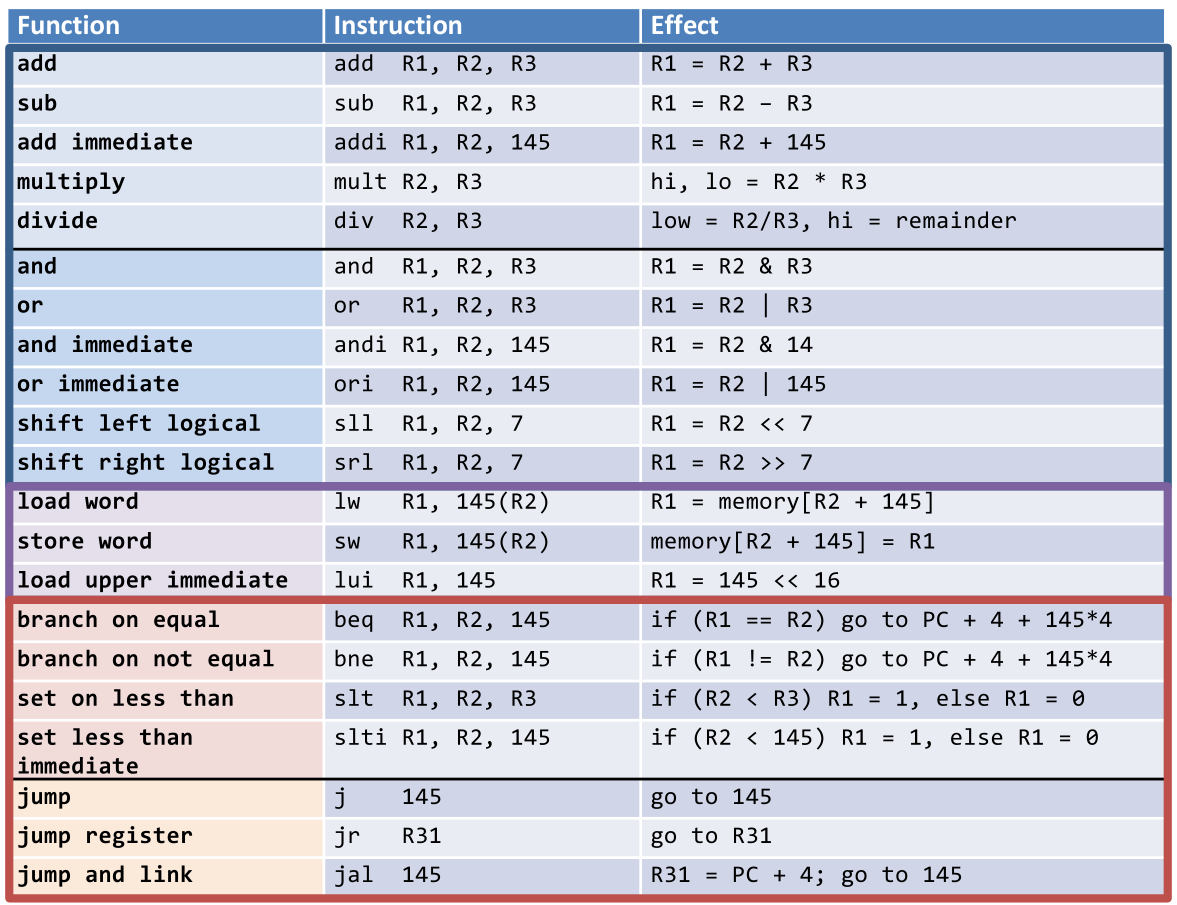
\includegraphics[width=16cm, height=13cm]{image/mips-tabel.png} 
    \caption{MIPS oporation tabel}
\end{figure}

\newpage

\subsection{Sequencing}
\begin{figure}[h]
    \vspace{10mm}
    \centering
    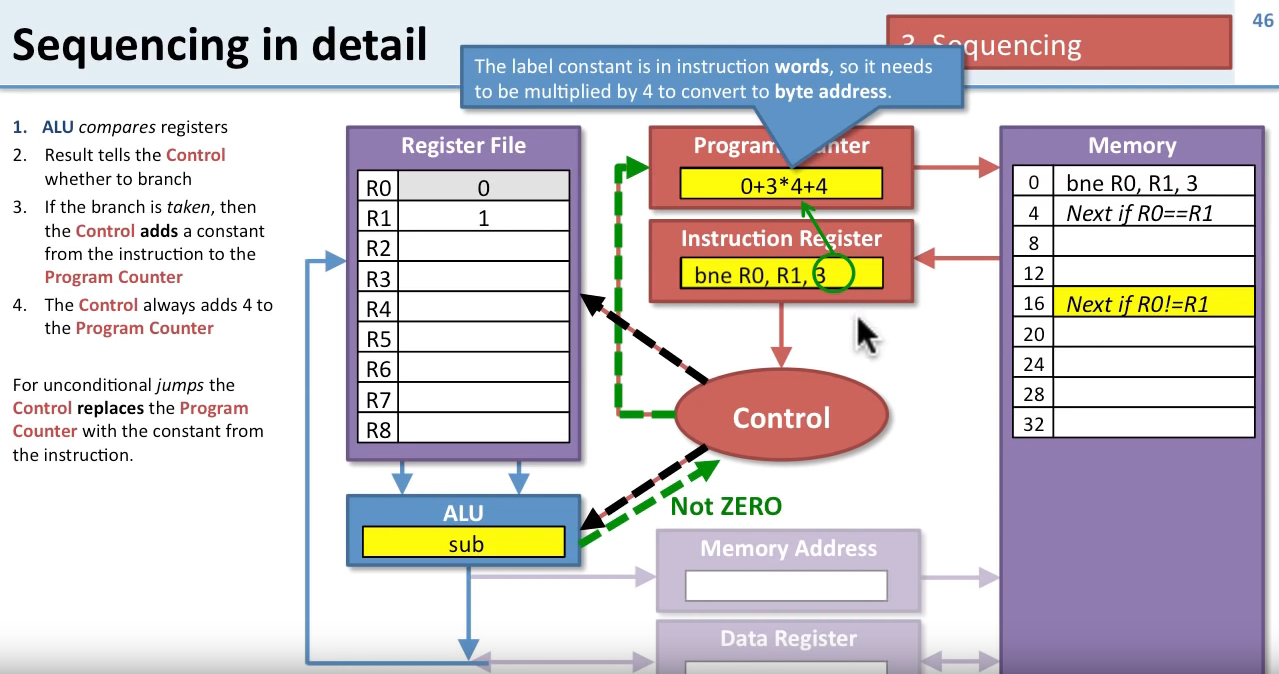
\includegraphics[width=16cm, height=10cm]{image/sequencing.png} 
    \caption{Sequencing}
\end{figure}
\newpage

\subsection{Converge to Assambly code}
\noindent\textbf{If Else example} \newline
\begin{figure}[h]
    \vspace{10mm}
    \centering
    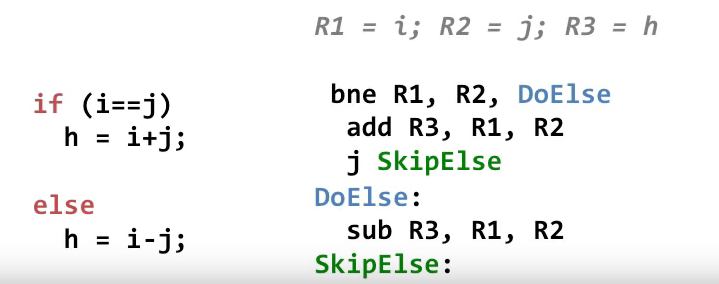
\includegraphics[width=10cm, height=5cm]{image/assambly-exampel.png} 
    \caption{Assambly exampel}
\end{figure}

\section{ISA2}
%https://inst.eecs.berkeley.edu/~cs61c/resources/MIPS_help.html
\subsection{MIPS type format}
\begin{itemize}
\item  R-format, Aretmetic and lodgical \newline
  op: ex add \newline
  rs: first register \newline
  rt: second register \newline
  rd: destination register \newline
  shmt: shift amount \newline
  funct: Function selector (add = 32, sub =34)
\item  I-format, Load/store, branch and intemidiats \newline 
  op: ex addi, beq \newline
  rs: first register \newline
  rt: second register \newline
  rd: inttediate value 
\item  J-format, Jump 
  op: ex j skipelse \newline
  rd: address   
\end{itemize}

\begin{figure}[h]
    \vspace{10mm}
    \centering
    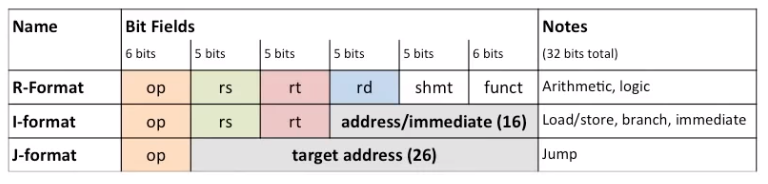
\includegraphics[width=17cm, height=6cm]{image/mips-types.png} 
    \caption{MIPS Types}
\end{figure}

A instruction allwas ends with 00 it means that when a instruction is done we update the program couner
to by 4 or more it changes the posistion of the 16bit intermidjet for i-format and can. (bne, beq)

\subsection{Procedure}
Procedure is how a function call is handeld. It is devided into two parts Caller and Callee,
the caller call the procedure (callee).
The oporation for contolling procedure is called jump-and-link (jal).
It stores the return address (PC+4) in \$ra (R31).
Where (ra = register address (updates automatically))
(PC = project counter)
(R31 = value).
jr \$ra returns the value.

\subsubsection{Stacking}
To avoid conflicts with writing over the callers register files, one uses staking in predefined
ranges to allow store data independent from the callers. 
(R29 =  store stack data \$sp)
When a register file is added the stock pointer is moved and when it is done it returns with (jr) and then
reset the previously used register files.
when it has used what it needs it removes them when leaded one value at a time


\begin{figure}[h]
    \vspace{10mm}
    \centering
    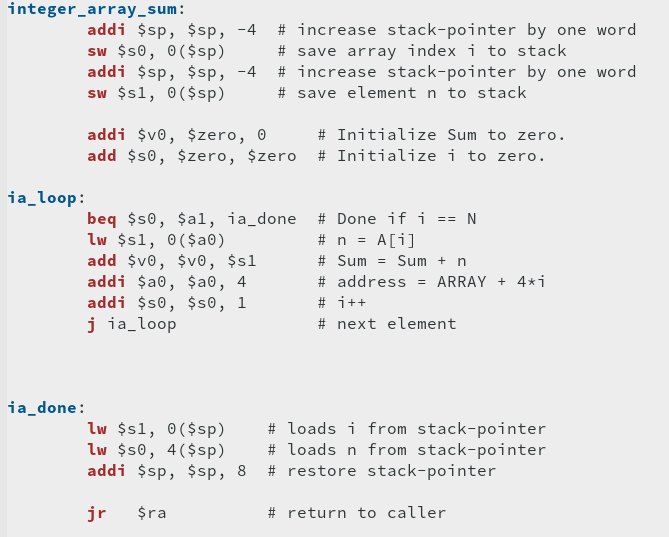
\includegraphics[width=16cm, height=12cm]{image/code-ex.png} 
    \caption{code ex}
\end{figure}

\begin{figure}[h]
    \vspace{10mm}
    \centering
    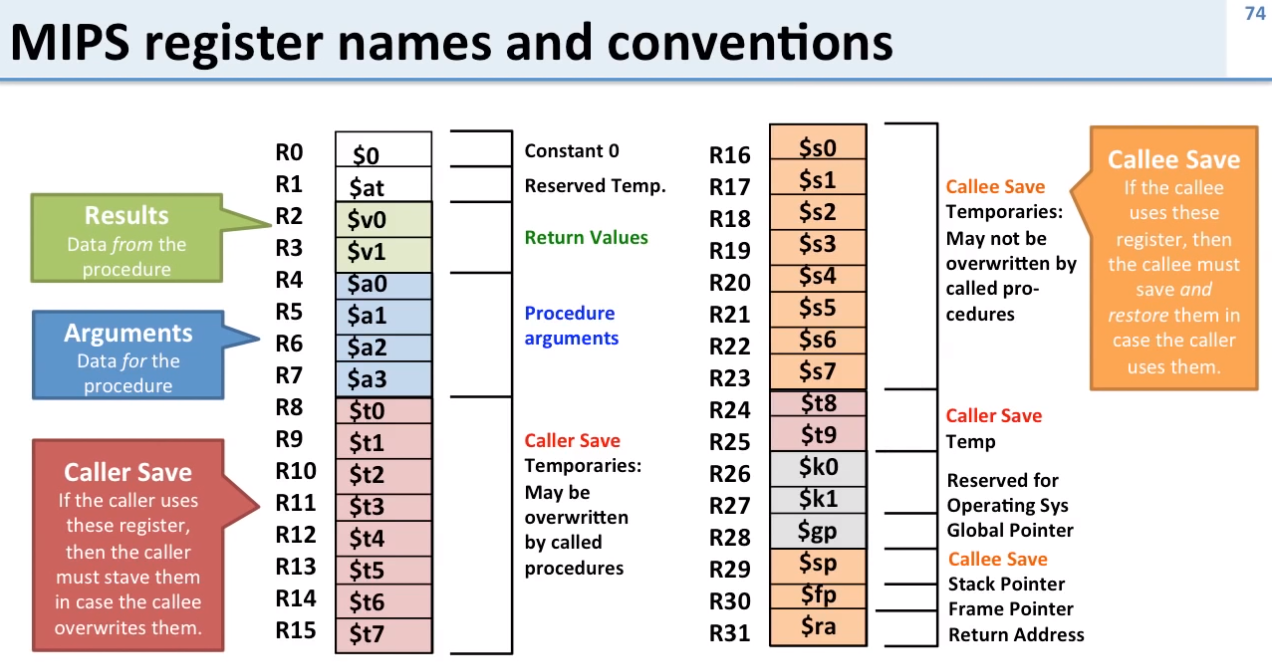
\includegraphics[width=16cm, height=8cm]{image/mips-register.png} 
    \caption{MIPS register}
\end{figure}

Notice that the register files for the callee save is \$sx and for the caller \$tx.

\newpage
\subsection{Other ISA}
\begin{figure}[h]
    \vspace{10mm}
    \centering
    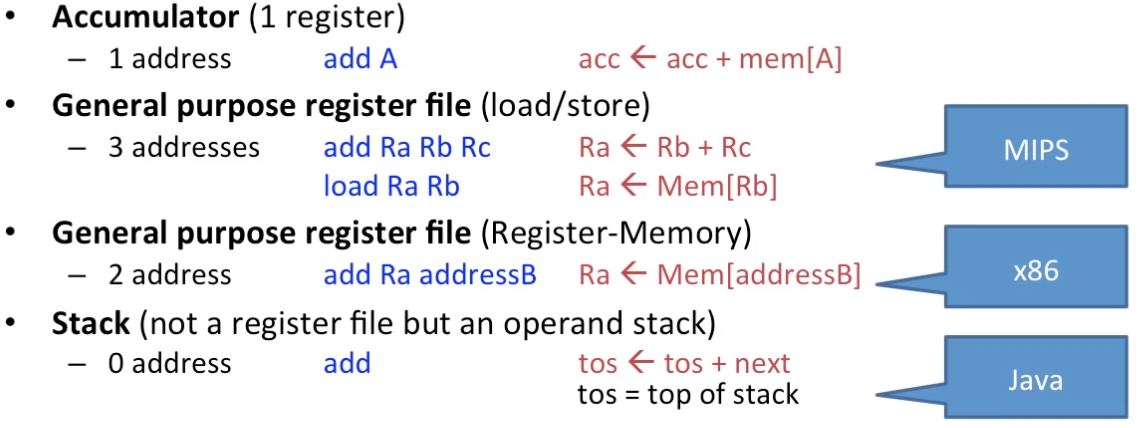
\includegraphics[width=16cm, height=6cm]{image/other-isa.png} 
    \caption{Other ISA}
\end{figure}

\begin{figure}[h]
    \vspace{10mm}
    \centering
    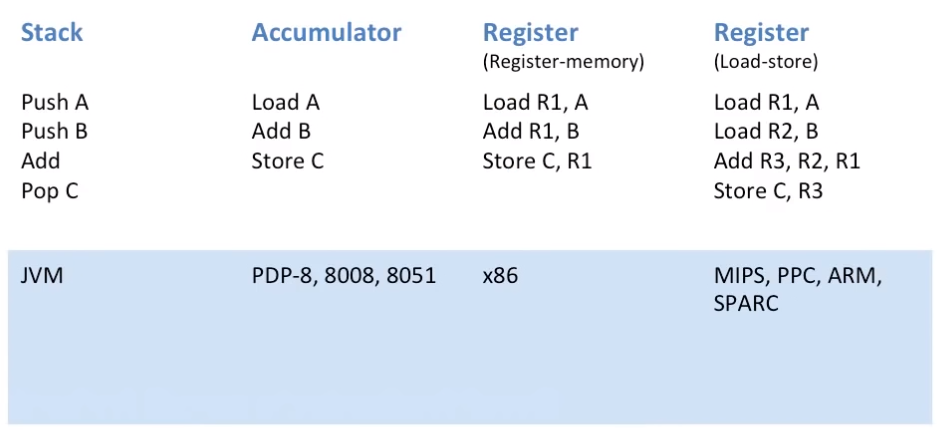
\includegraphics[width=16cm, height=6cm]{image/other-isa-instructions.png} 
    \caption{Other ISA instructions}
    \label{other-isa-instructions}
\end{figure}



\newpage


\section{Arithetic}

\subsection{Binary numbers}
\begin{itemize}
\item  Binary numbers reduses noice and disregard the exact voltitge to rusult in on off mode.
\item  In comuter sience octal and hexadecimals are also often used becose of it properties.
  every octo didgets represent 3 in decimal
  every hex didgets represent 4 in decimal
\item  msb=most significant bit
\item  lsb=lest significant bit
\item  Optemazation: $0010*0101$  2 oporations $\to 0101*0010$  1 oporations
\item  Multiplication: (fixed point need to shift desimal point)
  $0010 * 0101 = 0010 + (0010 shifting[00]) = 1010$
  $0011.010 * 0001.110 = $
\item  Addition: (Same for fixed points and integers)
  $1110+1000= carry[1] 0110$ Overflow
  $0101+0001= 0110$ Not overflow
\end{itemize}

\subsection{Negative integes}
\begin{itemize}
\item  \emph{Signed magnetude:} msb is the sign
  ${1011}_2 = {-(2+1)}_{10} = {-3}_{10}$
\item  \emph{tow's complement:} if msb is 1 then negative number every other digiet after is positiv
  ${1011}_2 = {-8 +2 +1}_{10} = {-5}_{10}$
\end{itemize}


\subsection{Oporations}

\subsection{Non integer numbers (Floating and fixed point)}
\begin{itemize}
\item  Converting binary to decimal:
  $0.111 = 1/2 + 1/4 + 1/8= 0.875$
\item  Fixed point: for defined ranges $1.001$ and $0.100$ one can chose large and small representations
\item  Floating point:  IEEE standard, se following image
\item  Standard floting point is in binary so FFFF is at most 1111 and with two's complement  0111
\end{itemize}

\begin{figure}[h]
    \vspace{10mm}
    \centering
    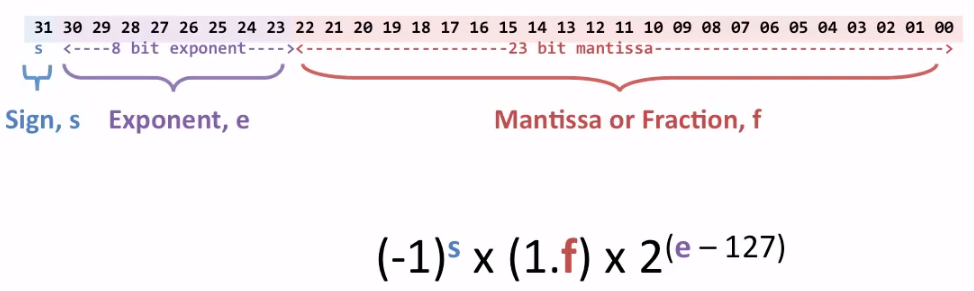
\includegraphics[width=16cm, height=5cm]{image/floating-point.png} 
    \caption{Floating Point}
    \label{floating-point}
\end{figure}

\subsection{Overflow}
\begin{itemize}
\item  input: msb = 1 for boath numbers and output: msb = 0 (overflow)
\item  input: msb = 0 for boath numbers and output: msb = 1 (overflow)
\item  input: msb = 0 for boath numbers and output: msb = 0 (Not overflow)
\item  input: msb = 1 for boath numbers and output: msb = 1 (Not overflow)
\item  input: msb = 1 and msb = 0 (Maby overflow)
\end{itemize}


\newpage

\section{Logic}
% https://aur.archlinux.org/packages/logisim/

\begin{figure}[h]
    \vspace{10mm}
    \centering
    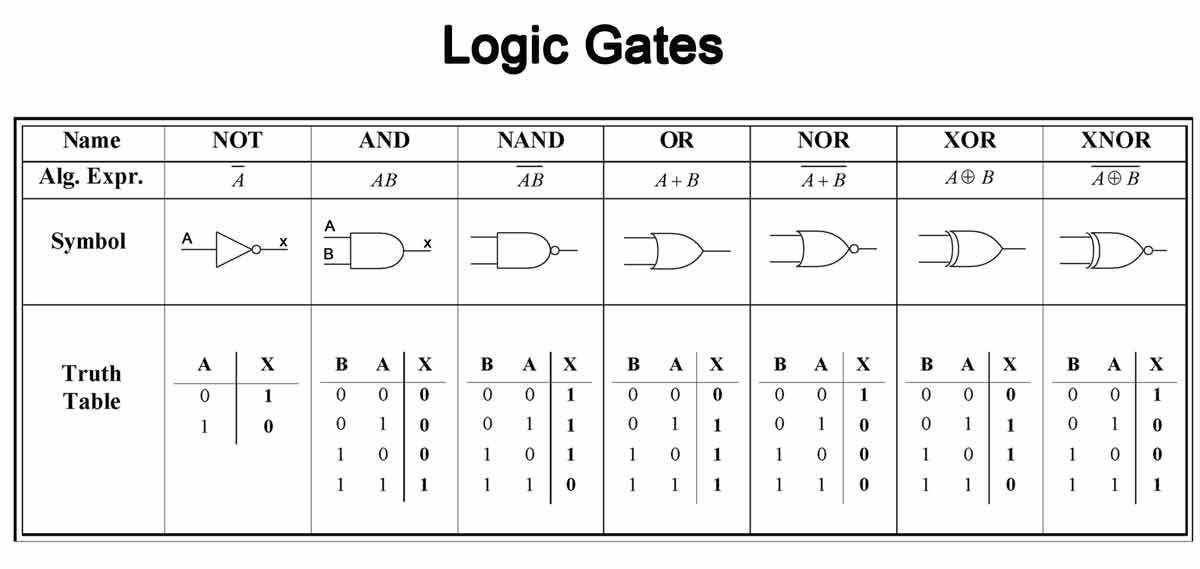
\includegraphics[width=16cm, height=8cm]{image/logic-gates.jpeg} 
    \caption{Floating Point}
    \label{logic-gates}
\end{figure}

\begin{itemize}
\item  truth table, is used to represent all possible inputs and then the corresponding output.
\item  To determined the possible schematics one can write for the input A and B ``!A and B''
  not A and B. One often get a unnecessary complexity, one can often simplify the schematics.
  It is only done with the inputs that have an output of one.
\item  De Morgan’s Law $!(A+B)=!A \cdot !B$ $+$ and $\cdot$ works the same way but are different.
\item  karno map is used to easily determine the schematics. It is a matrix. It is possible to use
  more inputs then two. In the matrix one locks at when output is one.
\item  a cabal with 4 wires can take 4 bits. Overflow needs one extra wire on output
\end{itemize}


\textbf{Building blocks}
\begin{itemize}
\item   Building blocks are the first layer of abstraction since one can not se the logical gates
  constructed of. For example add is a building block.
\item  Two types of logic, combinational and sequential.
  combinational: output just depends on input
  sequential: output deepens on the state. State is stored in memory update on clock.
\end{itemize}

\begin{itemize}
\item  MUXes (Mulitplexrs): choose input from a buss/ routing signal.
  2-bit decision for input 4-bit selection. Starts from position 0.
\item  DEMUXes (Demulitplexrs): oposit, take on signal and decides where it want to be sent to
  Buss is a multi-bit signal ``wire''
\item  Decoder: binary to hot, (adds a zero or one)? in arrays it can shose position
\item  Encoder: hot to binary, (reomve a zero or one)?
\item  Adders: adds carrys on extra bit to handel overflow
\end{itemize}

\begin{figure}[h]
    \vspace{10mm}
    \centering
    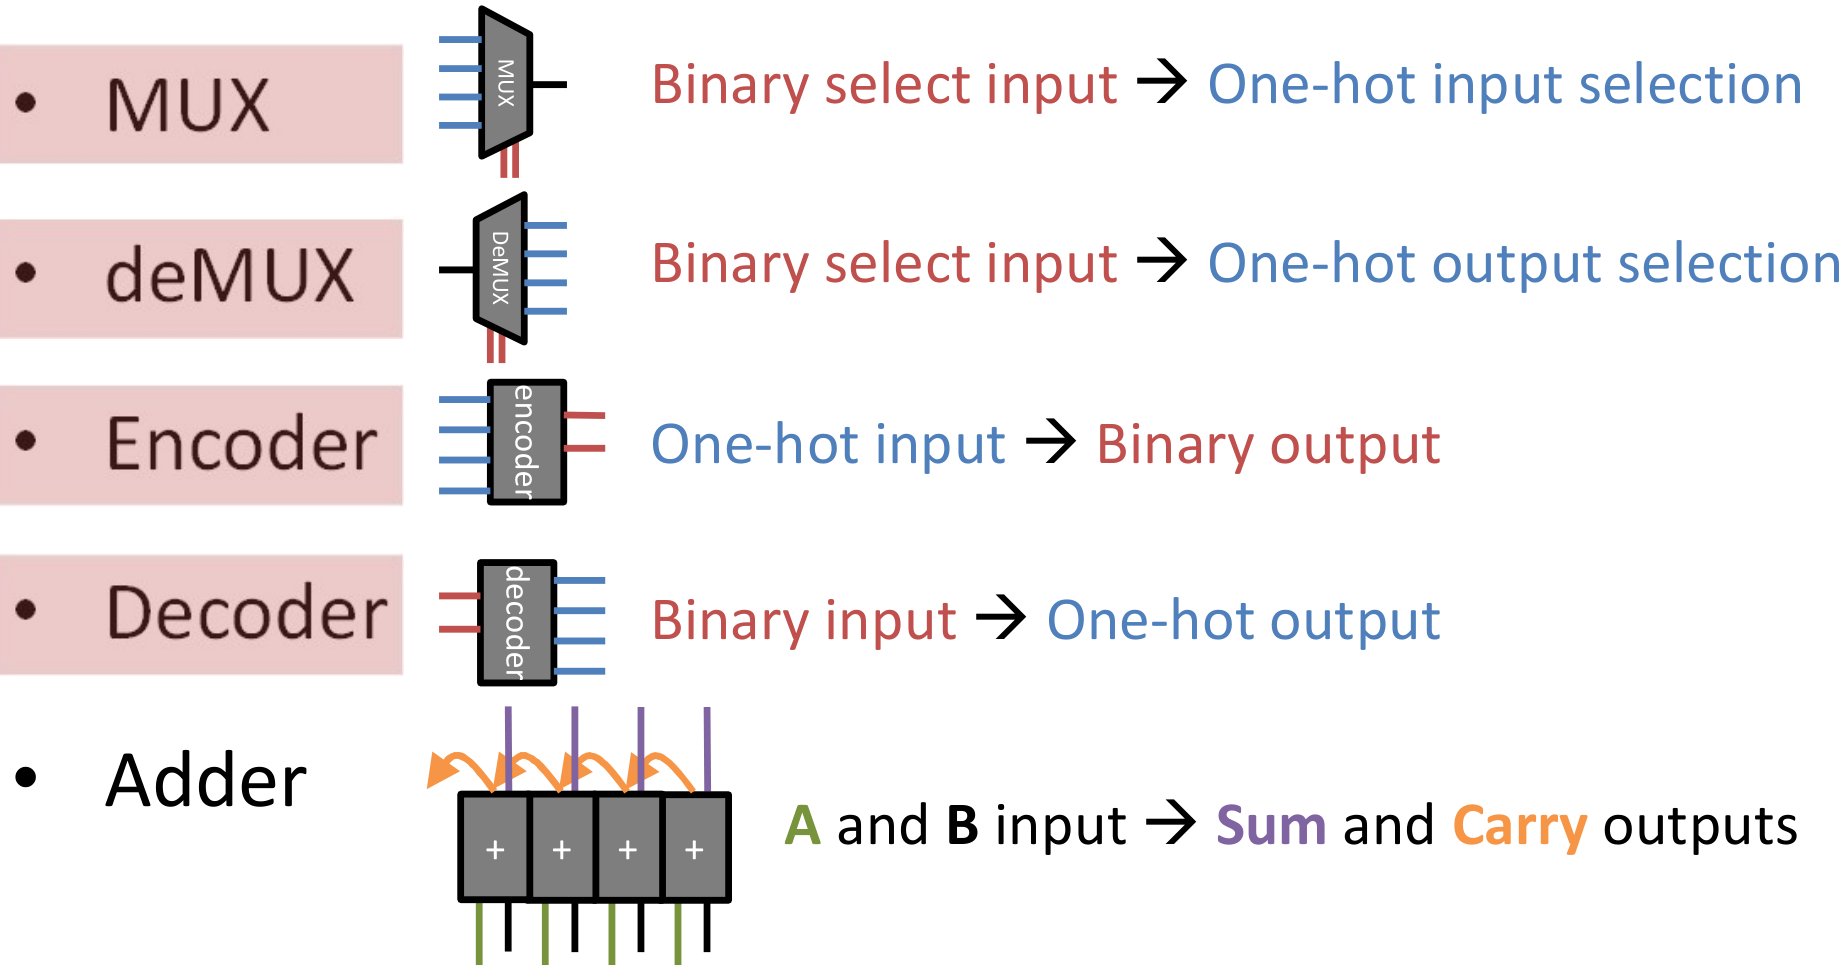
\includegraphics[width=16cm, height=8cm]{image/important-logic-blocks.png} 
    \caption{Floating Point}
\end{figure}

\textbf{Latches}
\begin{itemize}
\item  One use is for counters with a clock statest trigers the count.
  So when input is one the ouput is 0 and when the clock cliks it is one then when the input is
  0 the output is still 1.
\item flip flop: is a edge trigerd latche has a clock triger to open or close lathce and then can save it to SRAM cell
\end{itemize}

\begin{figure}[h]
    \vspace{10mm}
    \centering
    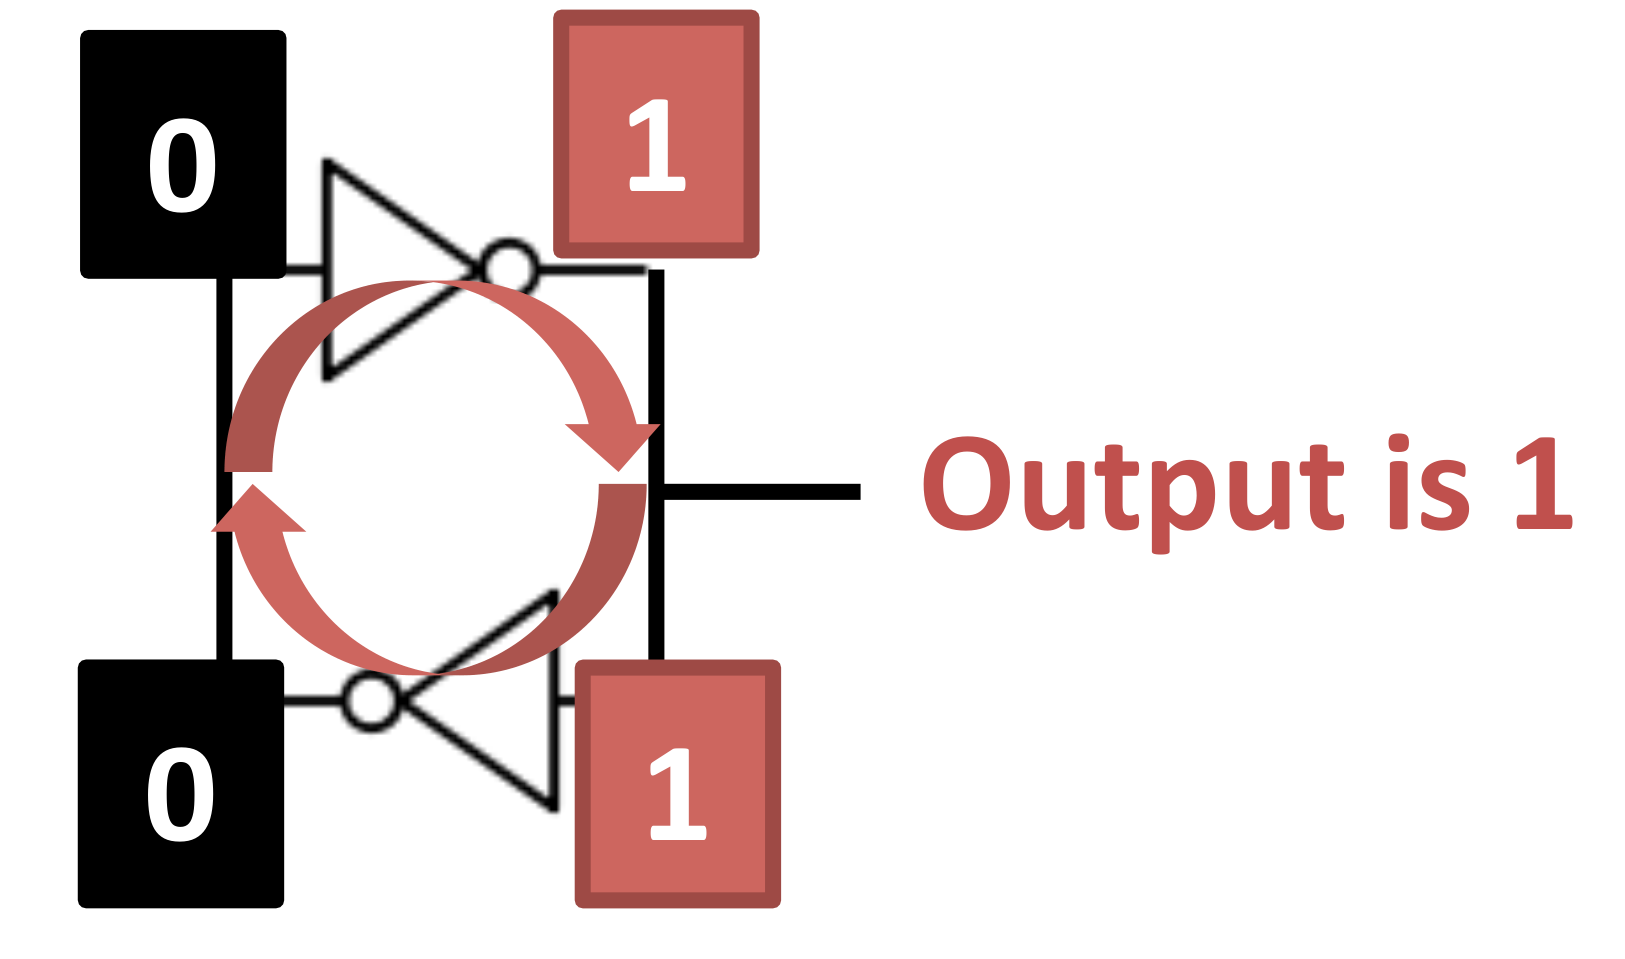
\includegraphics[width=16cm, height=8cm]{image/latche.png} 
    \caption{latche}
\end{figure}

\textbf{Memory}
\begin{itemize}
\item  SRAM (Static Random Access Memmory) Big, fast and expensive. Loops thou value in order to store it.
  To write to memory one uses a switch to update value.
\item  DRAM (Dynamic Random Access Memory) Smaller, Slower and cheaper. Uses a transistor to store value
  and a capacitor to store the charge so the data dose not disappear.
  That is why it is slower become the capacitor needed to be recharge
\end{itemize}


\newpage


\section{processor control and datapath}
There is 3 main part of the mips datapath as seen in the following image:
\begin{figure}[h]
    \vspace{10mm}
    \centering
    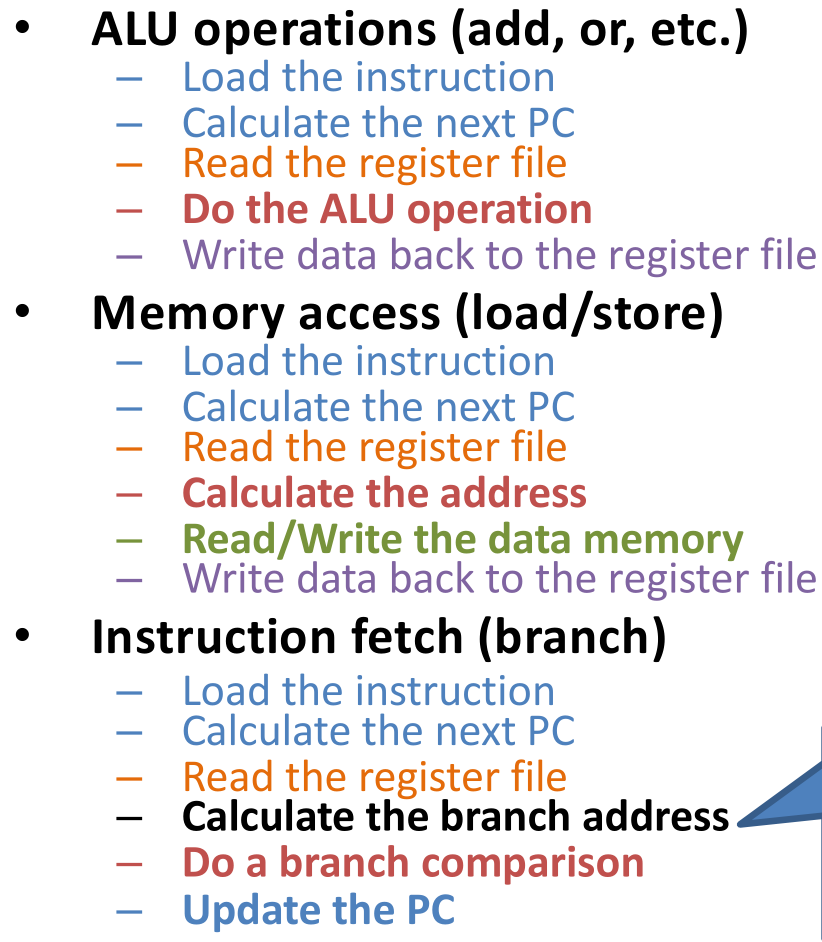
\includegraphics[width=12cm, height=14cm]{image/mips-datapath-3parts.png} 
    \caption{mips datapath 3 parts}
    \label{mips-datapath-3parts}
\end{figure}

\newpage

An overview of the mips datapath with j-format instruction:
\begin{figure}[h]
    \vspace{10mm}
    \centering
    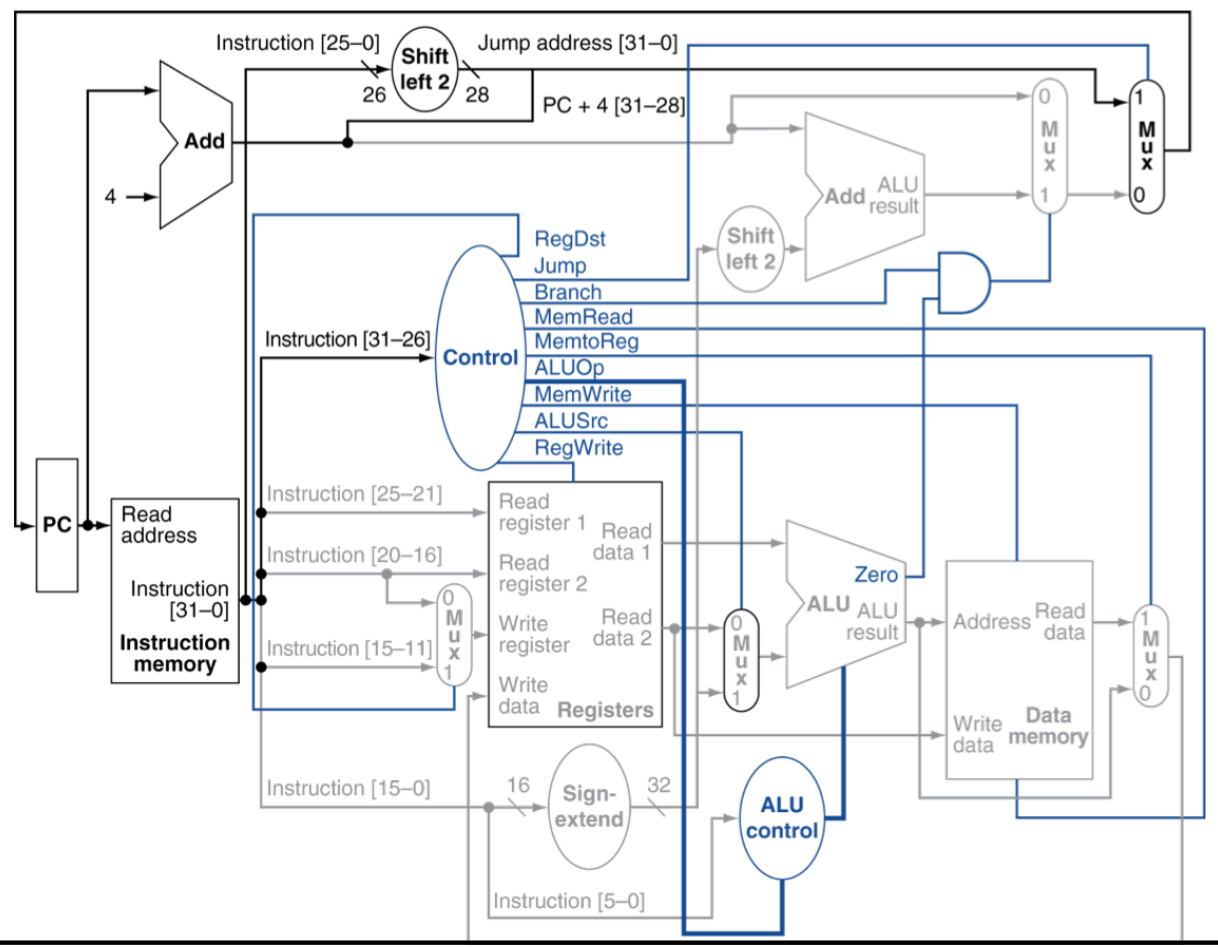
\includegraphics[width=16cm, height=12cm]{image/mips-datapath.png} 
    \caption{mips datapath}
    \label{mips-datapath}
\end{figure}

Think about the controler like a decoder that decodes the opt code from the diffrent formats.

\newpage

\subsection{Clock}
A clock is used to update the state and continu with the other instructions. Every state element uses
a clock. In mips prosesor clock gose to memory, pc, rf and dm. The clock unit is in (MHz) converting
from (ns) is simple. Ex 10ns: 1/10ns=0.1MHz.

\subsection{Critical path}
The longest path of the datapath is the critical path. Often PC is the fastest so one then calculates the
amount of time it takes for the instruciton has traveld the data path and reternd to know what the
critical path is. The longest part is data memory sinze it is big and slow. One often say read and write
takes constant time regardless of the amout of diffrent read and write.


\newpage


\section{pipline}
The perpus is to split a instruction cycle into multipe stages to run instructions in peralel to
improve preformans. Itch stage has its own pipline registerfile for storing the nessasary registers.
Pipline registers has a preforment reduction since it takes time, therfore more pipleine stages dose
not eqal greater proformens over a serten abount. One issue of preformans is balance the stages
inorder to get a good clock frequency. 
Not all stages are needed for eatch operation or instruction

\textbf{Mips stages}
\begin{itemize}
\item  IF= Instruction fetch
\item  ID= Decode and RF Read
\item  Ex= ALU Execute
\item  MEM= Memory
\item  WB= RF Write back
\end{itemize}

\begin{figure}[h]
    \vspace{10mm}
    \centering
    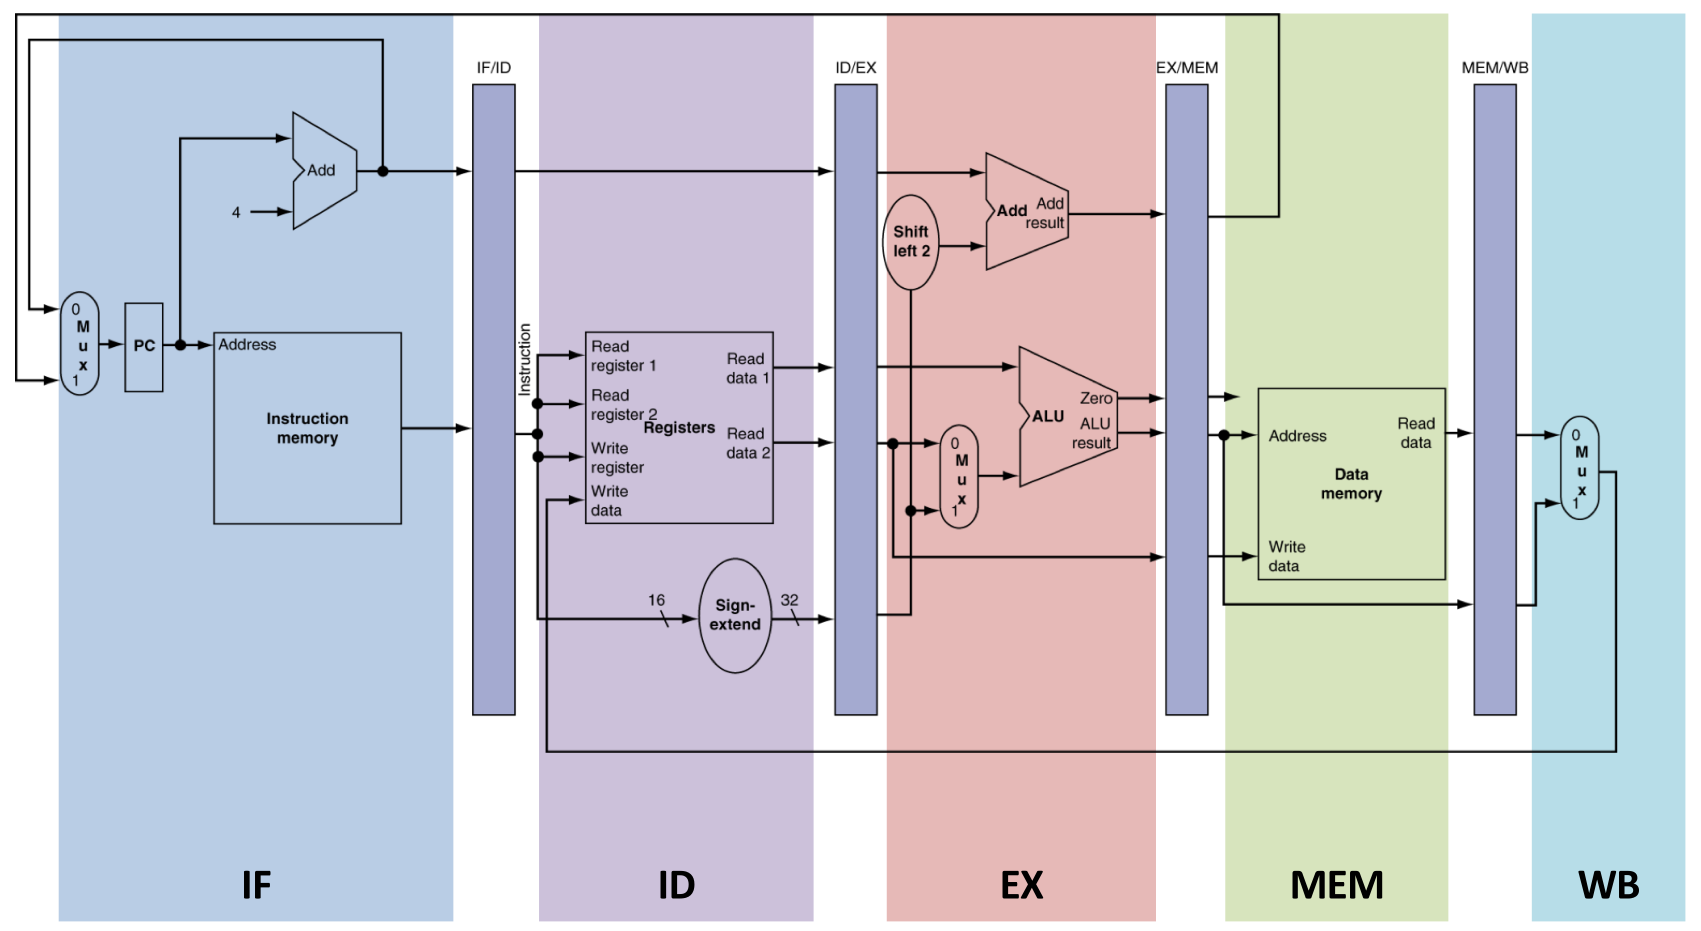
\includegraphics[width=16cm, height=8cm]{image/pipline.png} 
    \caption{Pipline}
    \label{pipline}
\end{figure}


\textbf{Terminology}
\begin{itemize}
\item  Bubbles= Is detected by the harwere where ther is no instuctions
\item  Nop= Is a sudo instruction for a stall type instruction (do not do anything)
\item  Delay slots= a stall type for branches. Try to fill in those slots with usful instructions.
\item  Interference= Can not read and write at the same time.
\item  Double pumping= Spiting write to first clock cycle and the second cycle is read.
\item  Forwarding= Getting data from a different pipeline stage from a register file.
\end{itemize}

\textbf{Calculating time coplexity}
\begin{itemize}
\item  overhead: (instructions time (ex 100ns)) / (stages (ex 1000)) + (regester overhead (1ns)) = 1.1ns \newline
    Total time: 1.1*1000
\item  Latancy: (stages* (penalty per stage) + original) \newline
  Latancy: (Time per instruction (ex 100ns)) + (pipline register's (ex 100-1))* (penalty per stage (ex 2ns)) = 300ns (3x slower)
\item  Trouput: (Time per instruction (ex 100ns))/ (Stages (ex 100-1)) + (Time pipline registes (ex 2ns)) = 3ns (every instuction is 33x faster) 
\end{itemize}


\newpage


\section{Pipline hazards}

\subsection{Data hazards}
\textbf{The issue}
\begin{itemize}
\item  Data is not available where we need it (later in the pipeline; not written back yet).
\item  Data is not available when we need it (need to read memory first).
\end{itemize}

\textbf{Fixing the issue}
\begin{itemize}
\item  Forward the data to where we need it.
\item  Stall if data is not ready yet (NOPs or Bubbles).
\end{itemize}

\begin{figure}[h]
    \vspace{10mm}
    \centering
    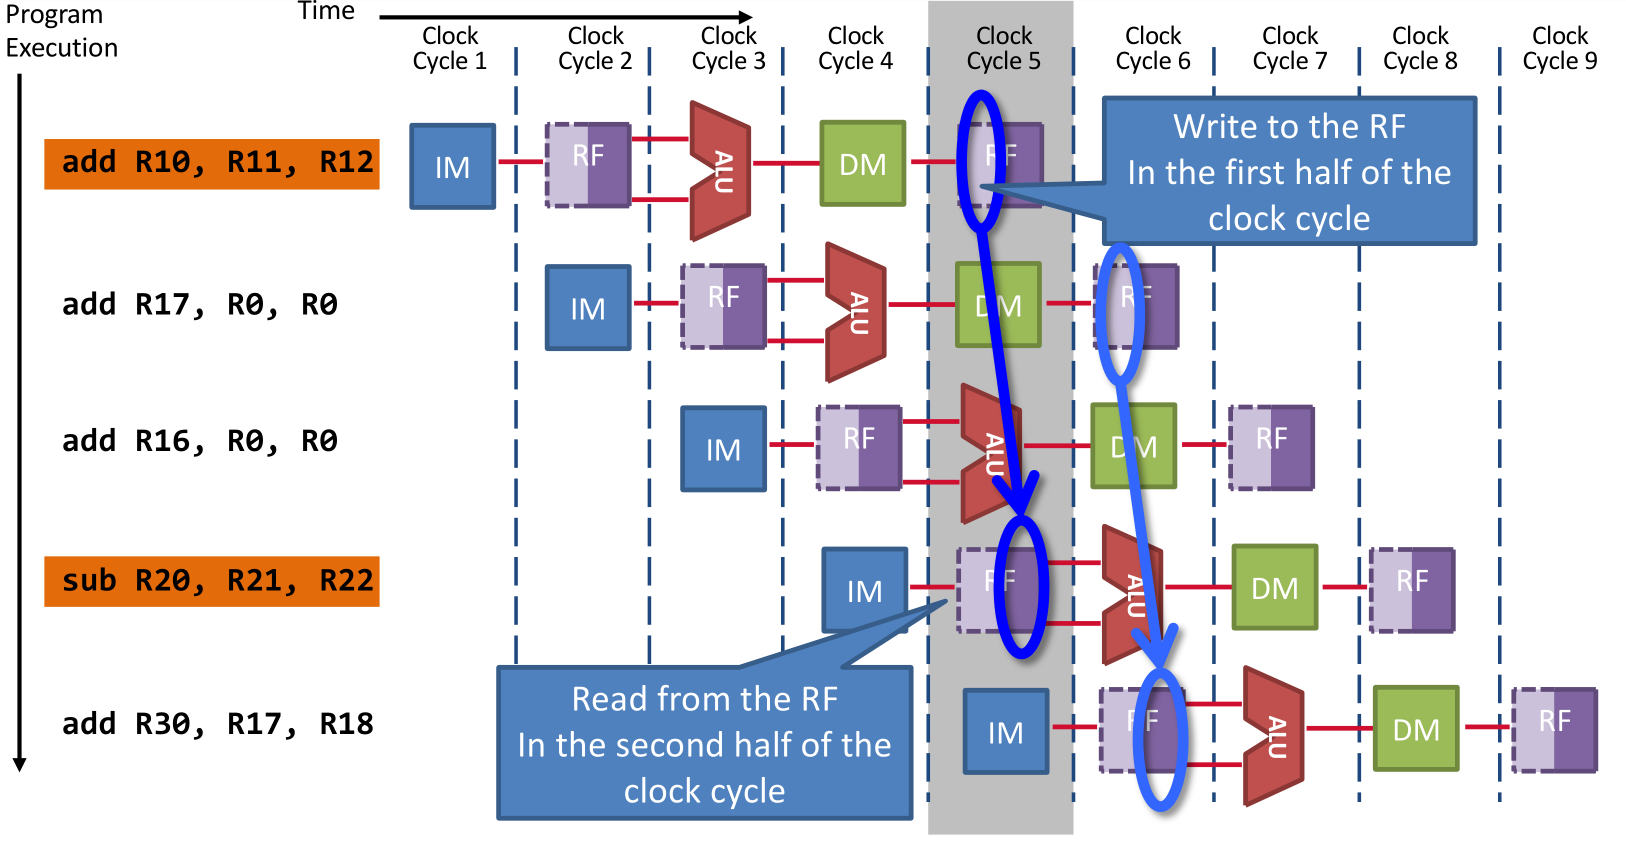
\includegraphics[width=16cm, height=8cm]{image/dubble-pump.png} 
    \caption{Dubble pump}
\end{figure}


\subsection{Control hazards}
\textbf{The issue}
\begin{itemize}
\item  Don’t know which instruction is next when we need to fetch it.
\end{itemize}

\textbf{Fixing the issue}
\begin{itemize}
\item  Calculate branch as early as possible.
\item  Stall with a branch delay slot.
\end{itemize}


\subsection{Structural hazards}
\textbf{The issue}
\begin{itemize}
\item  Can’t do the instruction because the hardware is busy.  
\end{itemize}

\textbf{Fixing the issue}
\begin{itemize}
\item  Build more hardware (double-pumped register file).
  Double-pumped write at the first hafe cycle and read at the other half
\end{itemize}

\textbf{Calculating time coplexity}
\begin{itemize}
\item  Branshe delay \newline
  (How many branches (ex 20\%)) / (How maney usful instuctions can be filled in (ex 50\%))
  = 20\%/0.5 = 10\%
\item  Cycles per instructions (CPI): (total cycles (with nop)) / (usful work (without nop))
  % https://www.youtube.com/watch?v=GAUppsLpjvg
\end{itemize}
%The amount of instructions that requires a NOP is 50% of 20% = 10% => 10% of instructions will take 2 cycles 
%This gives us a CPI of 10%*2+90%*1 = 0.1*2+0.9*1 = 1.1 CPI 
%Therefore, the slowdown due to the load delay-slots is 10%.


\newpage


\section{Predicting Branches and Exceptions}
When the prediction is wrong, clean up is needed.
– “Kill” or “Squash” so they don’t execute (they were wrong)
– Prevent them from writing: disable RegWrite, MemWrite in the pipeline
– Turn them into NOPs: change opcode to add R0, R0, R0 in the pipeline


\subsection{Static pridictors}
\begin{itemize}
\item  Predict alwas not taken
\item  Predict alwas taken
\item  Backwards-Taken, Forward-Not-Taken (BTFNT)
\end{itemize}


\newpage


\subsection{Dynamic pridictors}

The implementation of branch preditors look somthing like this:
\begin{figure}[h]
    \vspace{10mm}
    \centering
    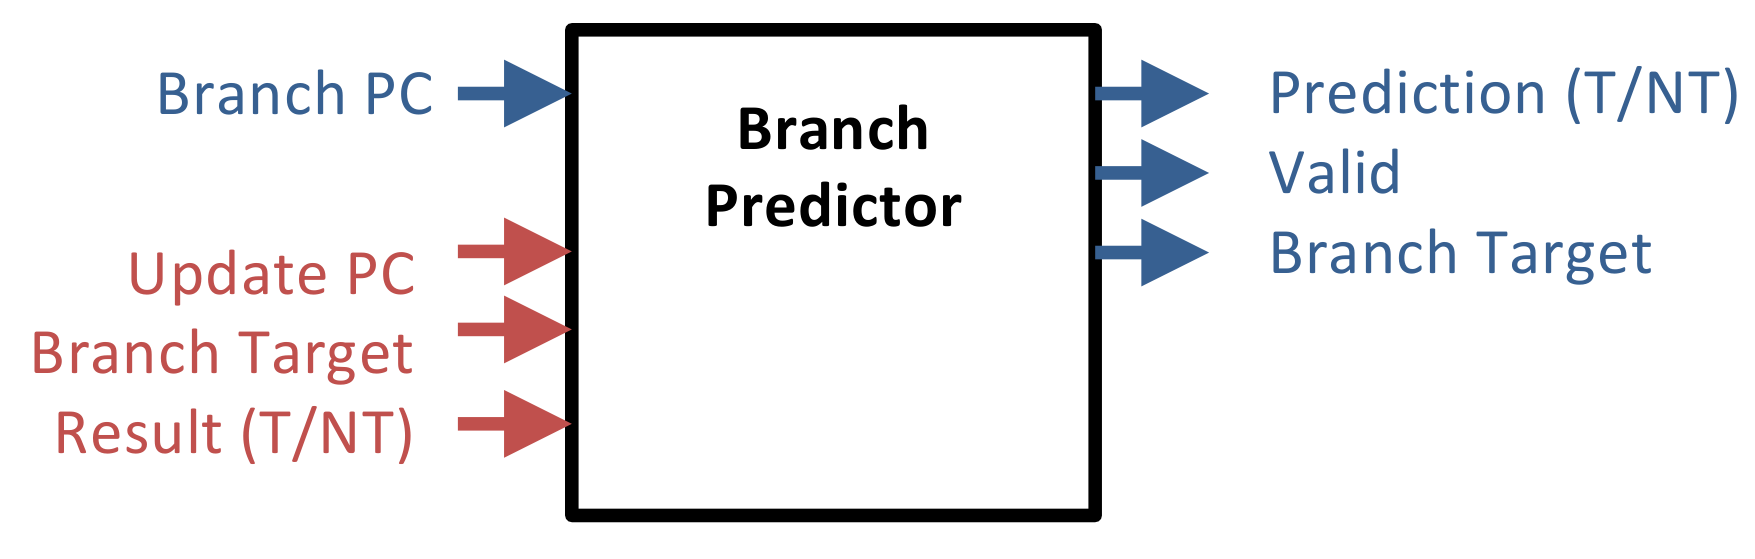
\includegraphics[width=16cm, height=5cm]{image/branch-predictor.png} 
    \caption{branch-predictor}
\end{figure}


\begin{figure}[h]
    \vspace{10mm}
    \centering
    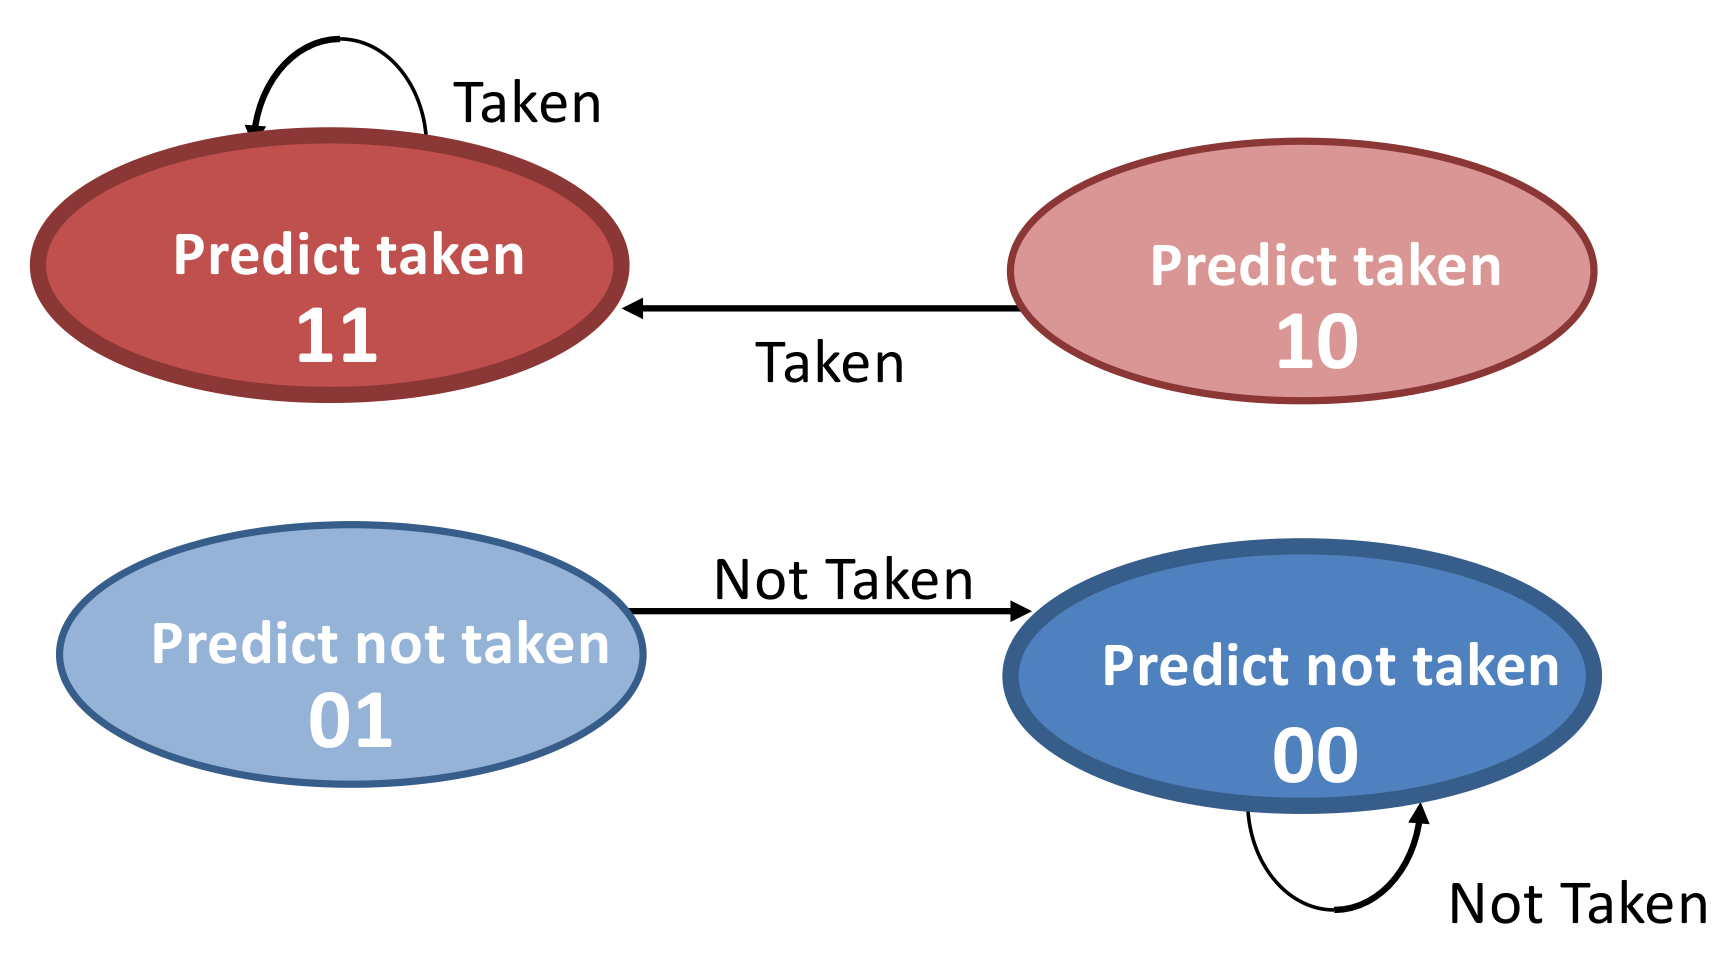
\includegraphics[width=16cm, height=10cm]{image/2-bit-predict.png} 
    \caption{2-bit predict}
\end{figure}

\newpage

\textbf{BTB}
\begin{itemize}
\item  Branch Target Buffer (BTB)
\item  Save a table with PC onorder to have history that we can predict on
\end{itemize}

\begin{figure}[h]
    \vspace{10mm}
    \centering
    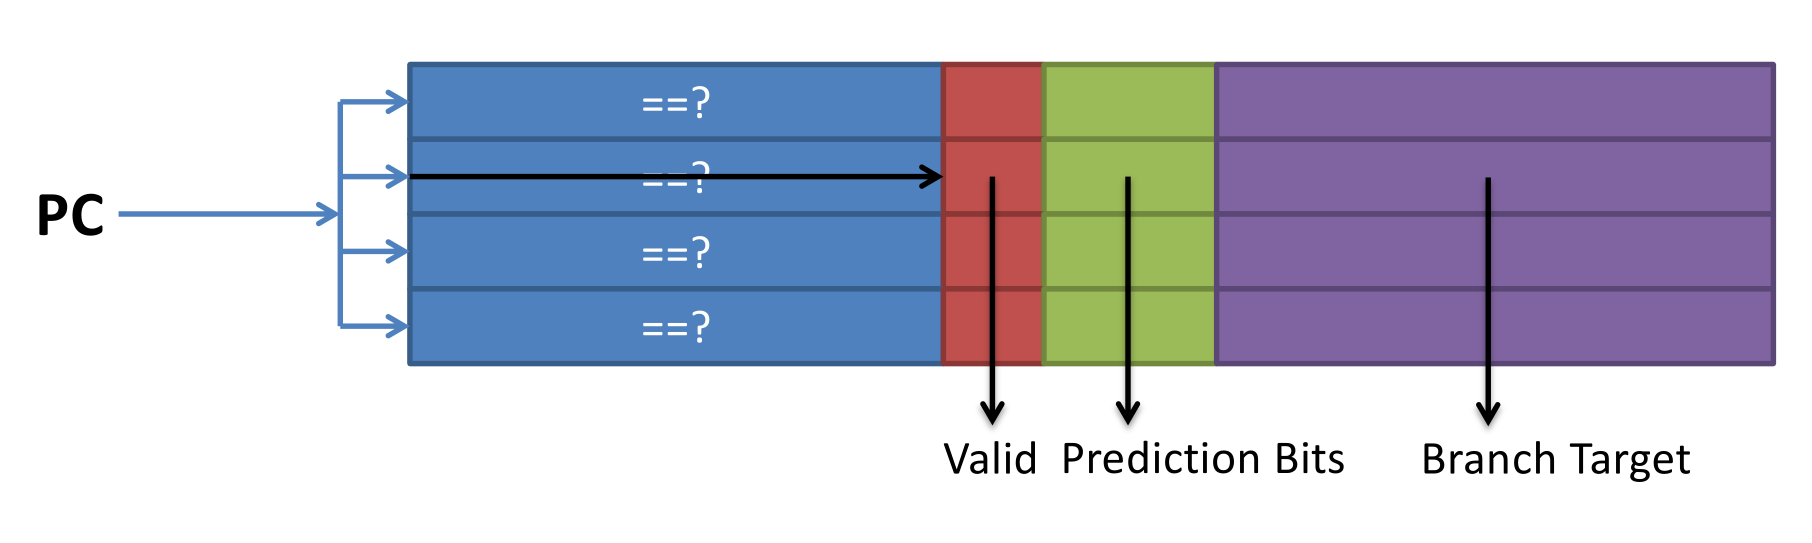
\includegraphics[width=16cm, height=5cm]{image/btb.png} 
    \caption{btb}
\end{figure}


\newpage

\subsection{Exceptions}
Exceptions are non-normal events that interrupt the normal flow of instructions
\begin{itemize}
\item  Divide by zero
\item  Misaligned memory access
\item  Page fault
\item  Memory protection violation
\end{itemize}

Interrupts are external events that interrupt the normal flow of 

\begin{figure}[h]
    \vspace{10mm}
    \centering
    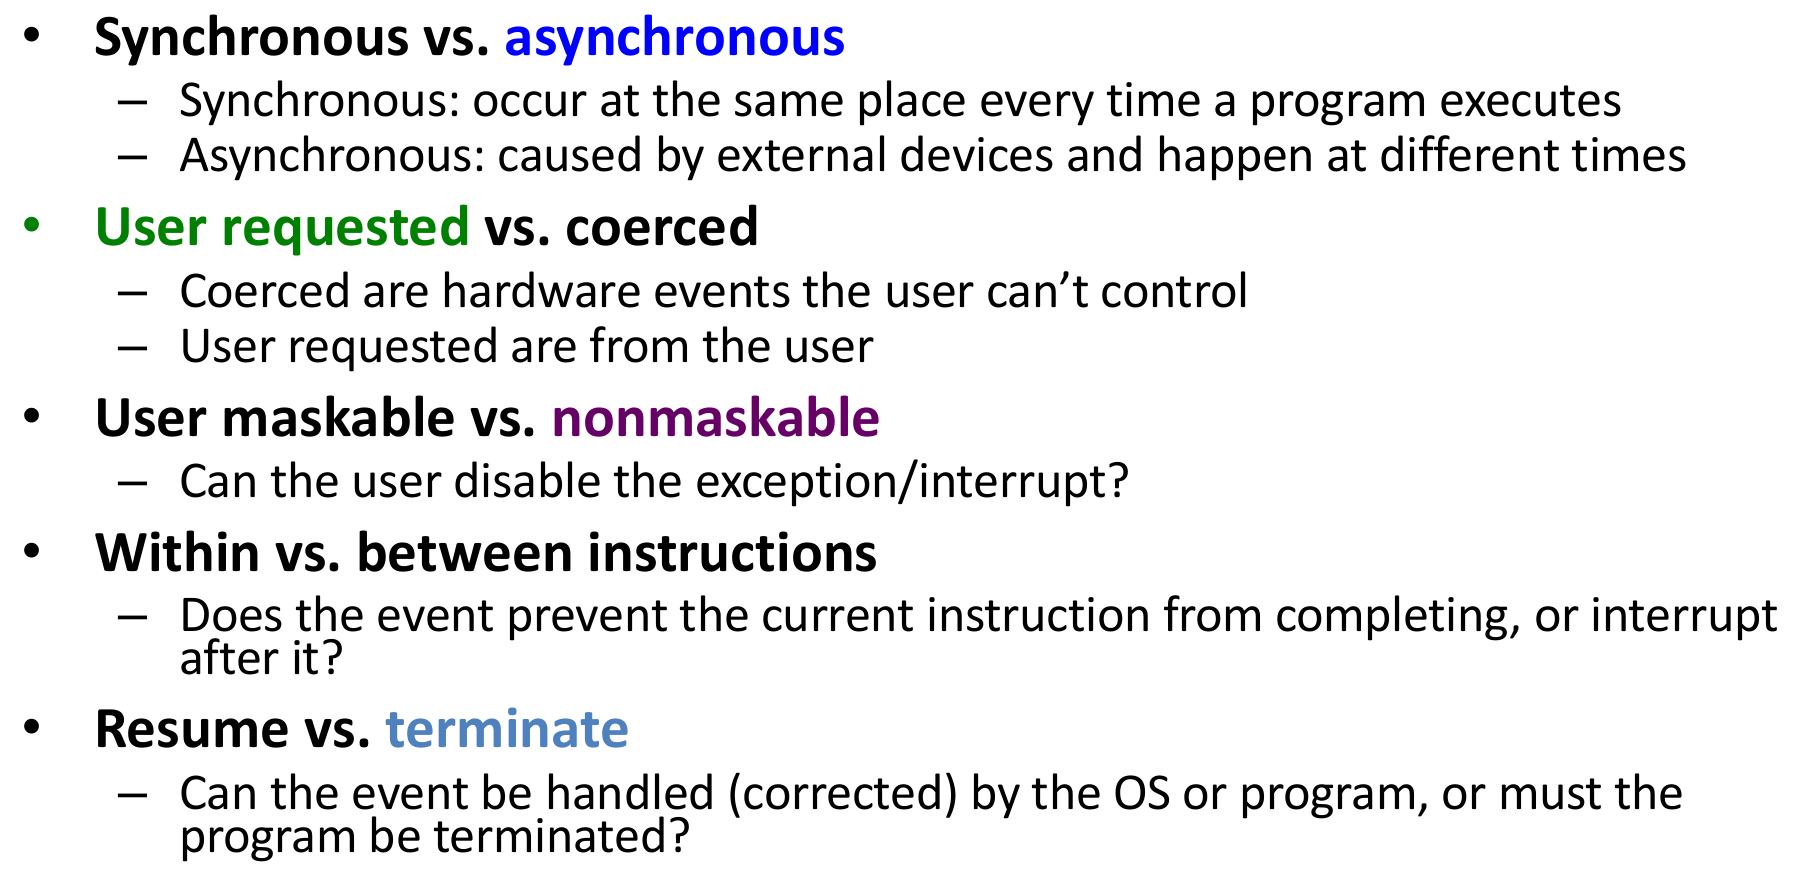
\includegraphics[width=16cm, height=9cm]{image/exceptions.png} 
    \caption{exceptions}
\end{figure}


\newpage


\section{Input/Output}

\textbf{Terminology}
\begin{itemize}
\item  nvram (flash): Simmiler to ram but it saves data when there is no power
\item  Busses:
  Parallel: many bits at once (e.g., 32 bits together in one clock)
  Used to be used everywhere
  Still used inside chips
\item  Serial links:
  Serial: one bit at a time (e.g., 32 clock cycles to send 32 bits)
  Used to be used only where distances were long (e.g., networks)
  Now used for most off-chip communications
\item  memory-mapped I/O:
  Manual handeling of I/O devices
  Map portions of the address space to I/O devices
  Read and write to those addresses to access the 
\item  direct memory access (DMA):
  Hardware who mange I/O devices (dynamicly)
\item  Polling:
  The device puts its status somewhere
  The OS repeatedly checks for it to change
\item  Interrupt:
  When the device is ready, it gets the processor’s attention by signaling an interrupt
  The OS then jumps to an interrupt handler to handle the event
\item  Througput: x/s
  The read and write speed
\item  Lateny: s/x
  Accesing time.
\item  Overhead:
  any combination of excess or 
  indirect computation time, memory, bandwidth,
  or other resources that are required to perform a specific task
\end{itemize}


\newpage

\textbf{Data transfers: manual copy}
\begin{lstlisting}%[language=Assembly]
addi R3, R0, 921600  // Number of copies
add   R2, R0, R0      // Counter starts at 0
loop:
  lw R4, 0x12f0(R0)  // Read the I/O device
  sw R4, 0xfe00(R2)  // Store the results
  addi R2, R2, 4       // Next location
  bne R3, R2, loop
done:
\end{lstlisting}


\textbf{Data transfers: DMA}
\begin{lstlisting}%[language=Assembly]
addi R1, R0, 0x12f0 // device address
addi R2, R0, 0xfe00 // destination
addi R3, R0, 230400  // number of words to copy
sw R1, 0x100b(R0) // set the device address
sw R2, 0x1008(R0) // set the destination address
sw R3, 0x1004(R0) // set the length and start
wait:
  lw R2, R0(0x1000) // Wait for it to be done
  bne R2, R0, wait
done:
\end{lstlisting}


\newpage


\section{Cache}
\subsection{Memory hierarchy}

\begin{figure}[h]
    \vspace{10mm}
    \centering
    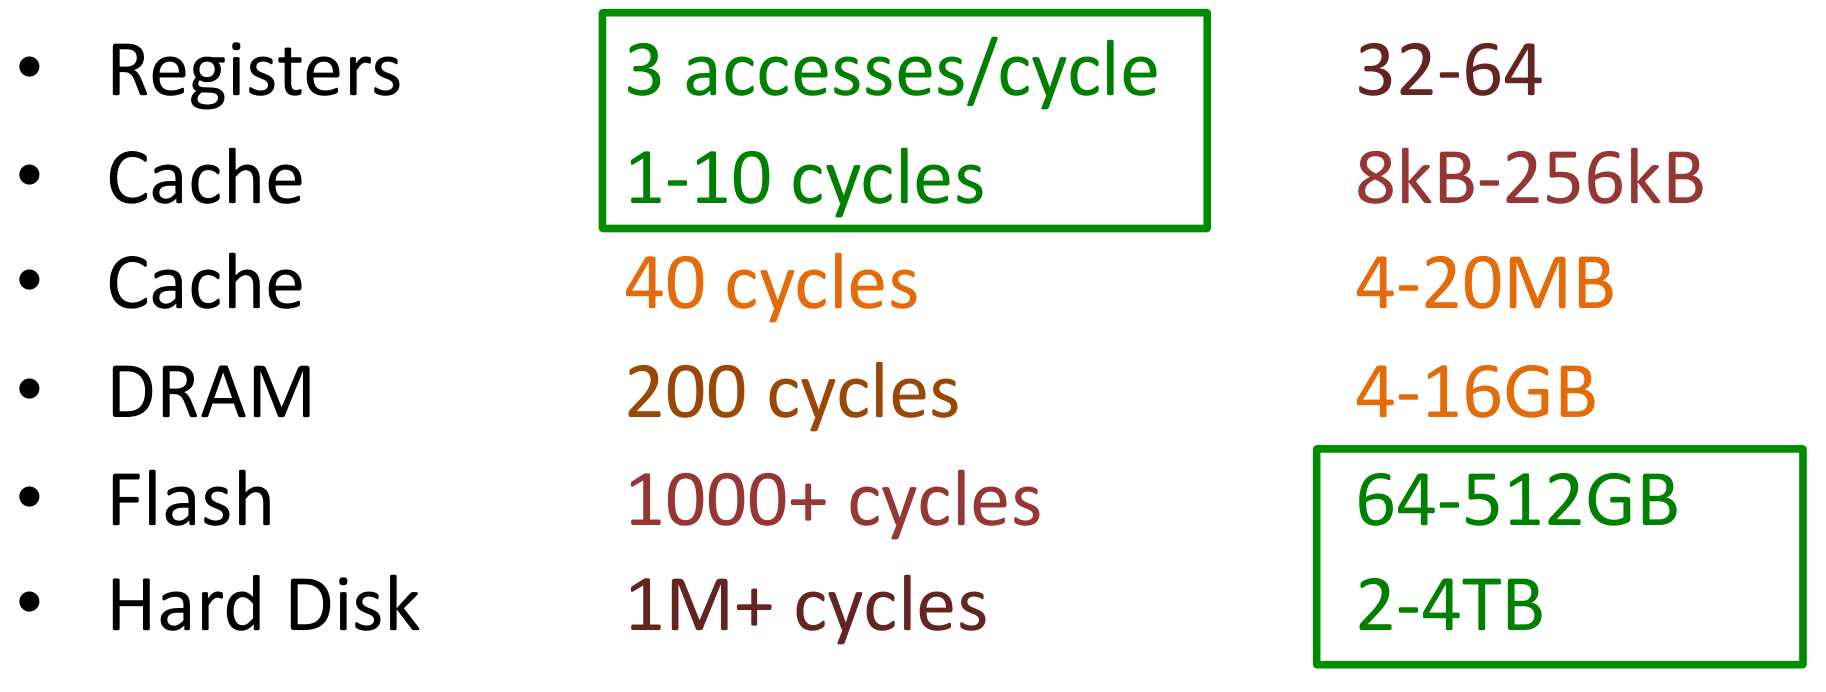
\includegraphics[width=16cm, height=7cm]{image/memory-hierarchy.png}
    \caption{memory-hierarchy}
\end{figure}

\textbf{3-types of cache types}
\begin{itemize}
\item  Fully-associative: Have to search all blocks, but very flexible 
\item  Direct-mapped: Only one place for each block, no flexibility
\item  Set-associative: Only have to search one set for each block,
  flexible because each set can store muliple blocks in its ways 
\end{itemize}

\textbf{Write policies}
\begin{itemize}
\item  Write-through: slow, simple 
\item  Write-back: fast (keeps the data just in the cache), more complex
\end{itemize}

\textbf{Termenology}
\begin{itemize}
\item  Data: What is being stored
\item  Tag: What address the data has
\item  Index: What we use to determen where we want to put the data
\item  Cache line (block) size: How many tag's there are
\item  Valid bit: If the data is correct
\item  Dirty bit: The data has been change and we need to write it to memory
\item  Type of cache: Fully-associative (FA), Set-associative (SA), Direct-mapped (DM)
\item  Replasment policy: Write-through, Write-back  
\end{itemize}


\textbf{Cache blocks}
\begin{itemize}
\item tag has 30bits and the 2 other bits is to determen what data
  63 bits for eatch entry 32bit data 30bit tag 1bit valid-bit 
\item larger block of data -> fewer tags -> more effeciant storage
\item 1 word cache block we have 1 32bit data
\item 2 word cache block we have 2 32bit data 
\item 4 word cache block we have 4 32bit data
\item we loade more data when we have space for it
  we will then have spatial locality
\item Last 2: determine the byte within the word   
\item Next N: determine which word in the cache block 
\item Remaining 32-N-2: tag
\end{itemize}

\textbf{Calculate overhead}
\begin{itemize}
\item  Data= Cache-Lines * Byte-Lines
\item  Overhead= Cache-Lines * (Tags-per-line + valid-bit)
\item  \% data=  Overhead / Data
\end{itemize}

\textbf{Calculate Address (Tag Index Offset)} %https://cs.stackexchange.com/questions/13356/how-to-calculate-the-number-of-tag-index-and-offset-bits-of-different-caches
\begin{itemize}
\item  Direct maped: \newline
  Offest= $\log$ (number of data blocks)  (+ 2-bit (4-bite cache block size if 64 then log 64)) \newline
  Index= $\log$ (number of cache lines) \newline
  Tags= 32(bit processor)- (Index+Offset) 
\item  x-set associative: \newline
  Offest= $\log$ (number of data blocks)  (+ 2-bit determens how the address looks like) \newline
  Index= $\log$ ((number of cache lines)/x) \newline
  Tags= 32(bit processor)- (Index+Offset)
\item  fully associative: \newline
  Offest= $\log$ (number of data blocks)  (+ 2-bit determens how the address looks like) \newline
  Index= 0 \newline
  Tags= 32(bit processor)- (Offset)
\end{itemize}

\begin{figure}[h]
    \vspace{10mm}
    \centering
    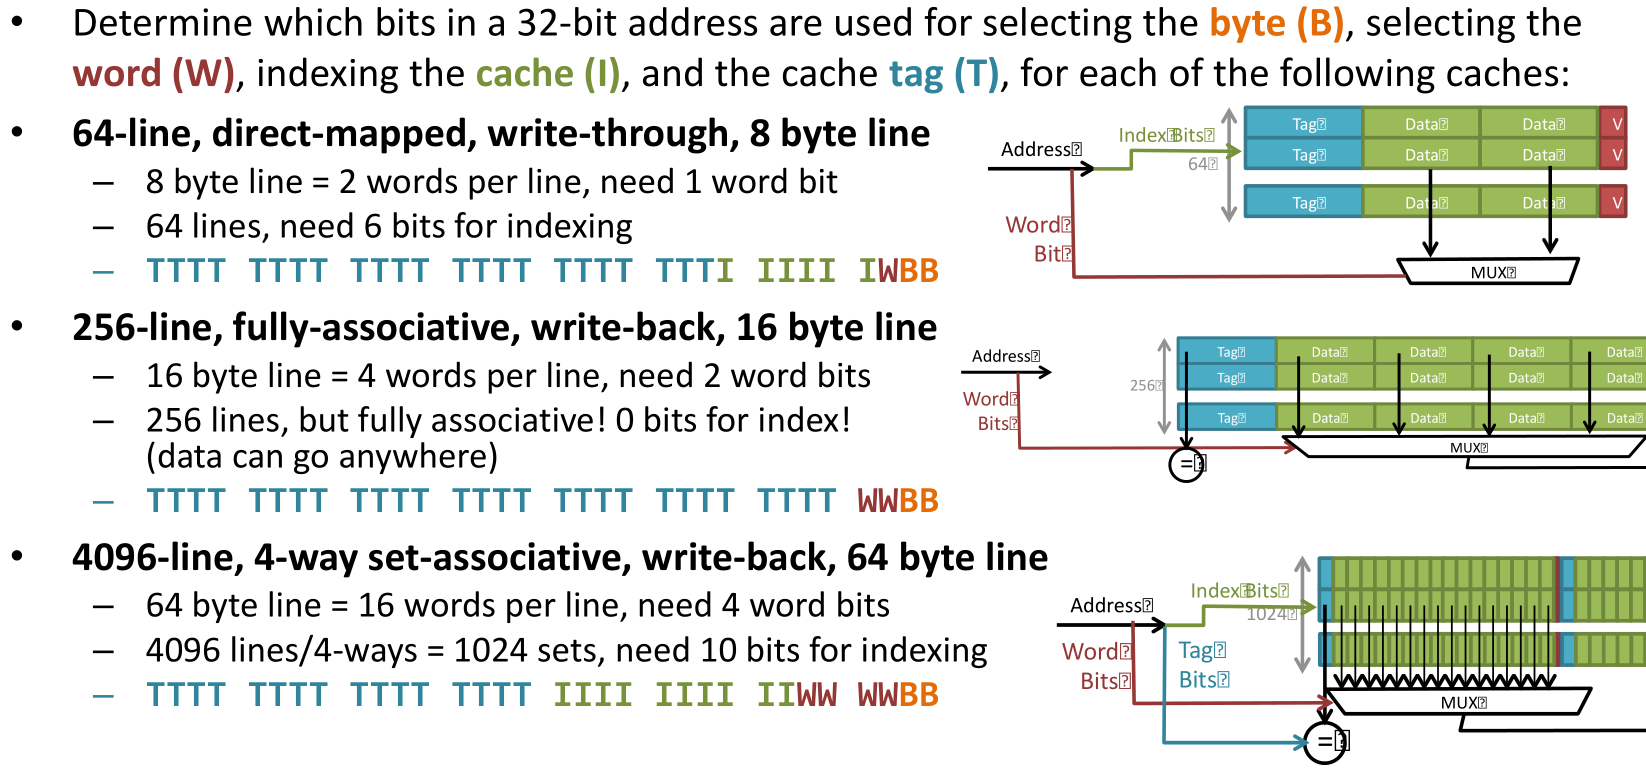
\includegraphics[width=16cm, height=7cm]{image/cache-format.png}
    \caption{cache-format}
\end{figure}


\textbf{Calculate Avrage memory access time}
\begin{itemize}
\item  Avrage-cycles= CacheL1*Cycles + CacheL2*Cycles + Dram*Cycles
\end{itemize}

\textbf{Mimimum assositivity}
\begin{itemize}
\item  (page size)/  ((Cache size)/ (bytes per line)) \newline
  ex: 8kB page size 64KB cache and 32bytes per line. log $(2^{13}/ (2^{10}/32)) = 8$  therfore 8-way
\end{itemize}

\subsection{Cache misses $3C's$}
% https://www.youtube.com/watch?v=OBp7rpdg_IQ
\begin{itemize}
\item  cold/compulsory miss: When the program first begin it dosent have enything in the cache
\item  conflicts miss: to small to store the nessesary data
\item  capasity miss: mapes at the same block an then overite unessesarly 
\end{itemize}


\newpage


\section{Virtual Memory}
\textbf{Why use VM}
\begin{itemize}
\item  Map memory to disk (“unlimited” memory)
\item  Keep programs from accessing each other’s memory (security)
\item  Fill holes in the RAM address space (efficiency)
\end{itemize}

\textbf{Termonology}
\begin{itemize}
\item  Translation= map address
\item  Page tables= for each program keep track of all translations
\item  Fine grain= page table with spesific address
\item  Coarse grain= page table with adress maped ranges
\item  Page Table Entries (PTEs)= number of translation  
\item  Translation Lookaside Buffer TLB= All of the pages, fast translation via hardware
\item  VA= Virtual program addresses
\item  PA= Physical RAM addresses
\item  Page offset= point to a range and then use the offset to determen where
\item  Translation Lookaside Buffer (TLB)= page table cache (Faster)
\item  Multilevel page table translation= page table point to other page tables (inseption)
\end{itemize}

\newpage

\textbf{Combining TLB and cache}
\begin{itemize}
\item  Physical caches: slow and needs the translation first and then save get the PA
  also known as Pysical-Index, Physical-Tagged (PIPT)
\item  Virtual caches: fast uses only virtual addresses, no translation, difficult for protection
  also known as Virtual-Index, Virtual-Tagged (VIVT):
\item  Virtual-Index, Phisically-Tagged (\textbf{VIPT}): VA for index PA for tags, fast dose translation and
  fetch from cache at the same time, most commonly used.
  We need a comperitor to se if the PA tags from cache matches the TLB PA onlny then we can say if we had a hit or a miss.
  The VA offset is what the PA tag is selected and the VA tag (number of virtual pages) is what the TLB uses.
  Mostly used for L1 cache not L2.
\end{itemize}

\textbf{TLB}
\begin{figure}[h]
    \vspace{10mm}
    \centering
    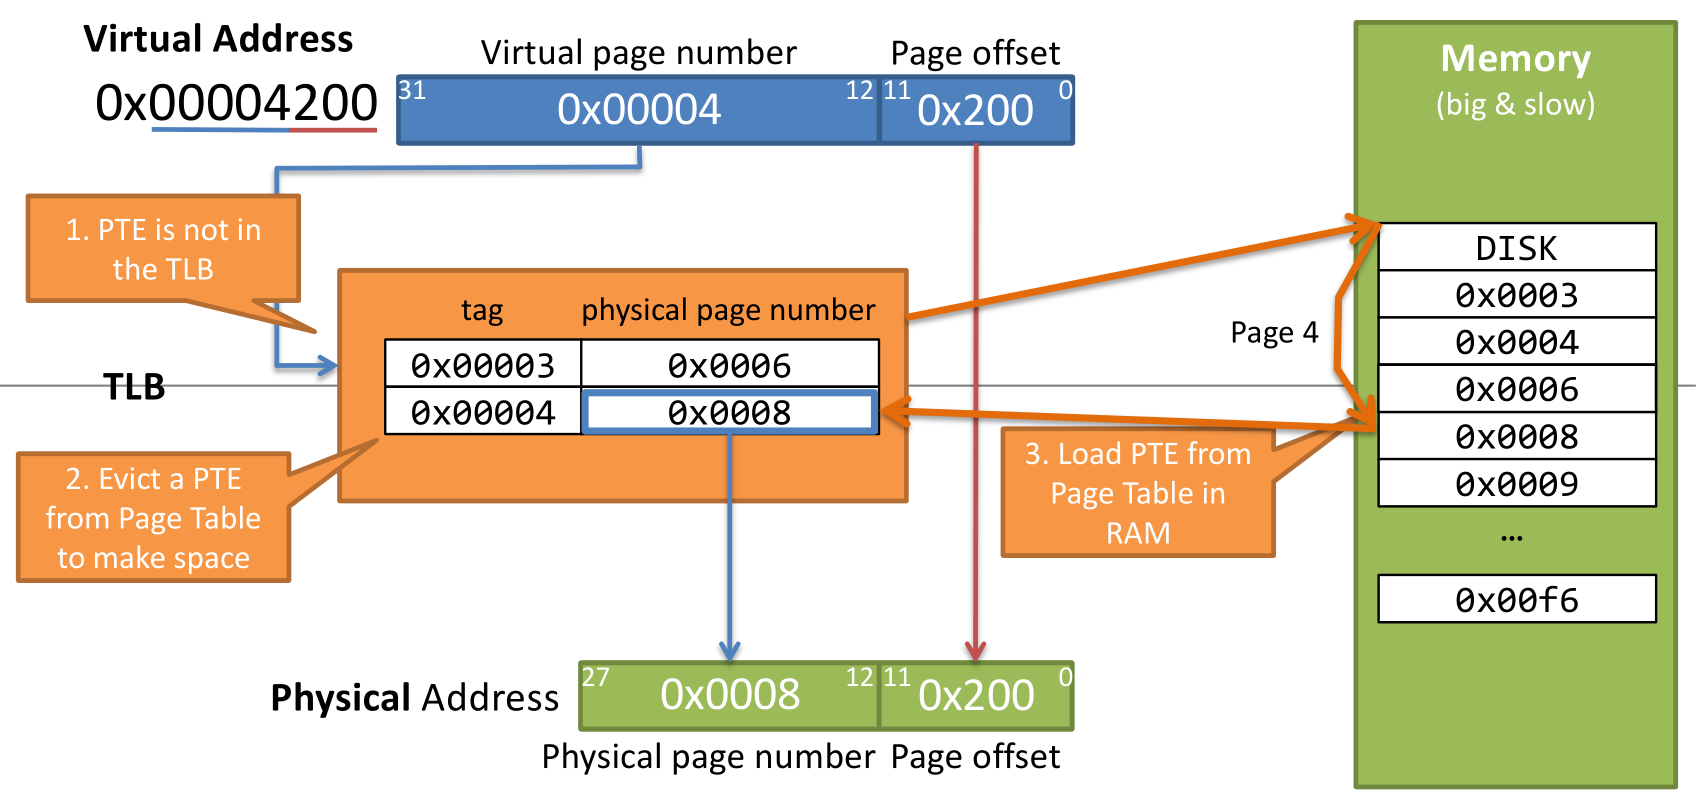
\includegraphics[width=16cm, height=7cm]{image/tlb.png}
    \caption{tlb}
\end{figure}

\newpage

\textbf{usful conversion: $2^n=xB$}
\begin{figure}[h]
    \vspace{10mm}
    \centering
    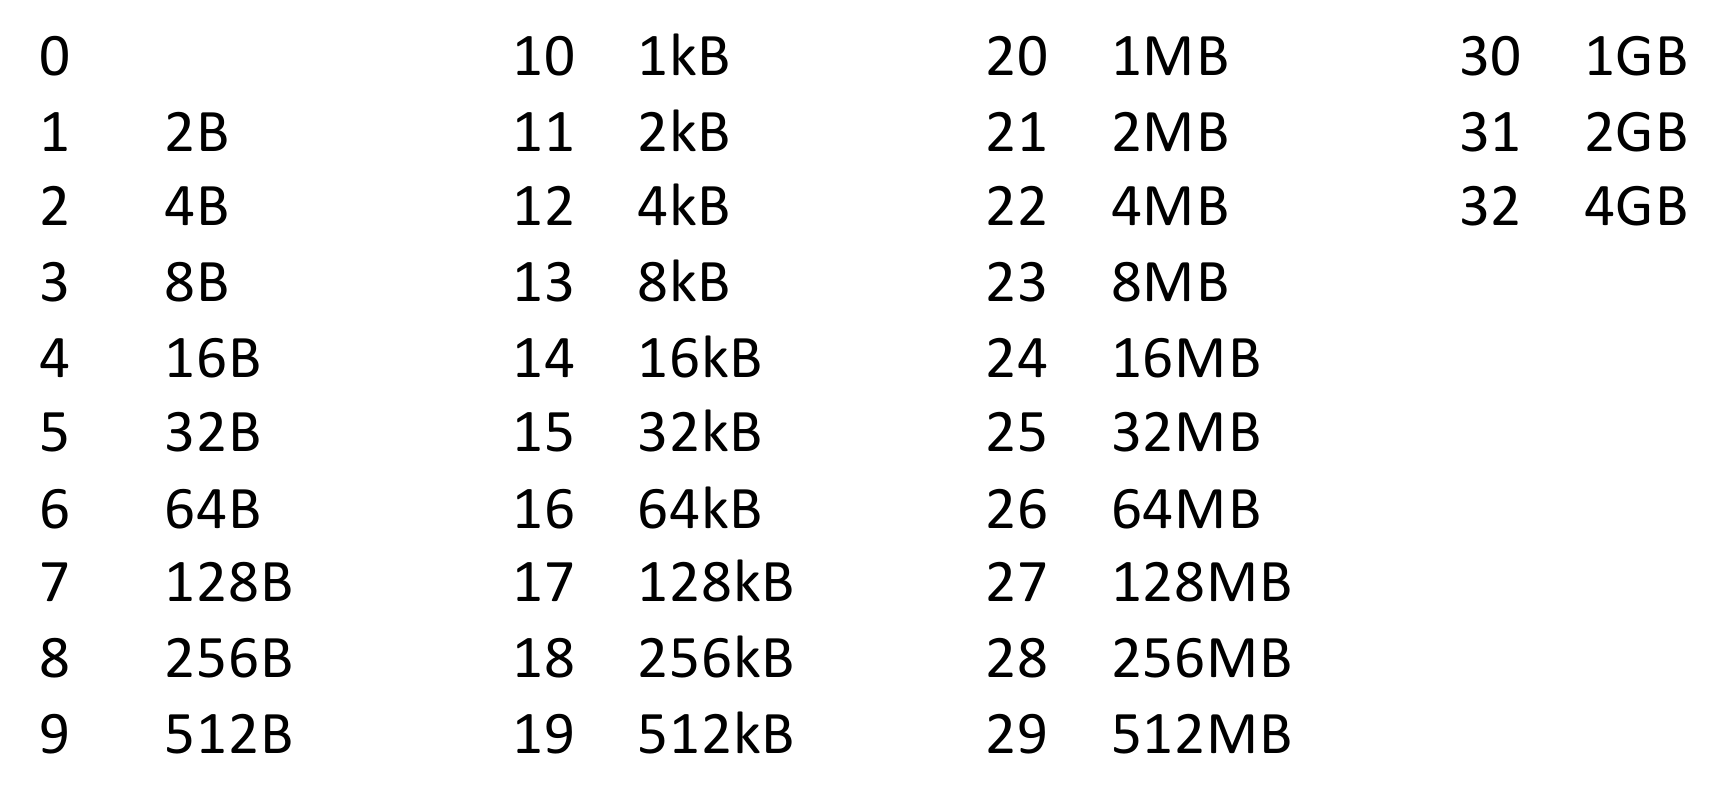
\includegraphics[width=16cm, height=7cm]{image/conversion.png}
    \caption{conversion}
\end{figure}


\textbf{Calculating Page sizeing VIPT}
\begin{itemize}
\item  Number-of-Virtual-Pages= $2^{32}/(pages)$  (in a 32bit address)
\item  Bits-used-for-Page-Offset= $\log$(pages)
\item  Bits-used-for-VPN= 32(bit prossessor)- Bits-used-for-Page-Offset
\end{itemize}

\textbf{Calculating TLB size}
\begin{itemize}
\item  TLB-size=Entries*Pages
\end{itemize}


\newpage


\section{Parallism}

\subsection{Multicore}
\textbf{powerwall}
\begin{align*}
  &\quad P=CV^2f \\
  &\quad C= \text{ capasiter, smaller transistors smaller capasiters} \\
  &\quad V= \text{ voltage, decressing makes it slower} \\
  &\quad f= \text{ frequancy, redusing clockspeed} \\
\end{align*}

\subsection{Paralel programing}


\textbf{Avrage prosessors}
\begin{align*}
  &\quad  \text{Calculate how many cores are used in avrage we need to know } \\
  &\quad  \text{how chunks (work) there is in total } \\
  &\quad  \text{how many time units (cycles think of a reverste peramid)} \\
  &\quad  \\
  &\quad  \text{there is 16 input data and we have 8-cores, we want to calculate the total sum} \\
  &\quad  \text{what is the avrage prossesor being used} \\
  &\quad  15 chunks, \; 4 time units \Rightarrow 15/4 = 3.75 \\
\end{align*}

\textbf{parallel issues}
\begin{itemize}
\item  Most programs can not utalise parellelism, need to devid the program to diffrent exicutions.
\item  We also need to share cache and therefore have proformanshe issue since we cant use the entire cache.
\end{itemize}


\textbf{How mutch faster}
\begin{align*}
  &\quad  75\% parallel, \; 25\% non parallel \text{ we have hundred thousend cores } \\
  &\quad  \Rightarrow  \text{Parallaism takes } (0.75/100000 + 0.25*1) \\
  &\quad  \text{Singuler takes } (0.75*1 + 0.25*1)  \Rightarrow 4* \text{ faster} \\
  &\quad  \\
  &\quad  \text{Speedup with Amdahl's law } Speedup=\frac{1}{(1-P)+P/S} \\
  &\quad  P= \text{ Parallel aktion} \\
  &\quad  S= \text{ Speed up of the parrallel part} \\
  &\quad  \Rightarrow \frac{1}{(1-0.75)+0.75/100000} = \frac{1}{0.25+0}= 4 \\
\end{align*}
%\subsection{Multicore issues}


\subsection{Syncronaziation}
\begin{itemize}
\item  Fix the issue with 2 prosessors accesing the same value att the same time.
\item  We can use atomic swap to first set lock to 1 then check the data.
\end{itemize}

\newpage

\textbf{locks}
\begin{figure}[h]
    \vspace{10mm}
    \centering
    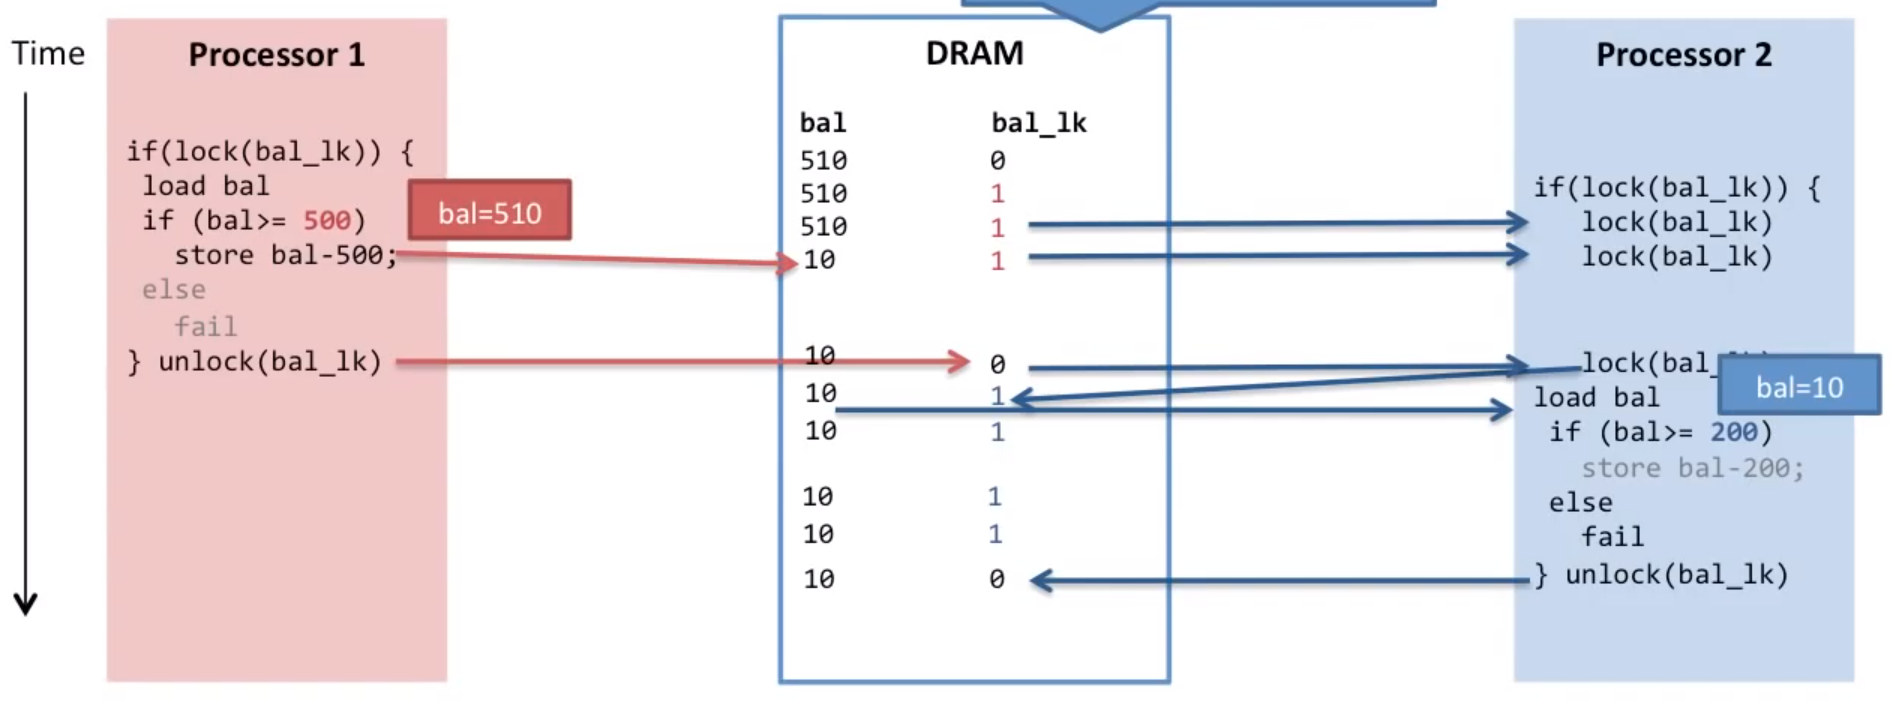
\includegraphics[width=16cm, height=7cm]{image/locks.png}
    \caption{locks}
\end{figure}


\subsection{Cache coherency}
\begin{itemize}
\item  How we use caches to save memory
\item  Locks: if the data has been accesed. (not a garanty of protection)
\item  Snooping: Look what the other processors are storing in there private cache   
\end{itemize}
  

\textbf{snooping}
\begin{figure}[h]
    \vspace{10mm}
    \centering
    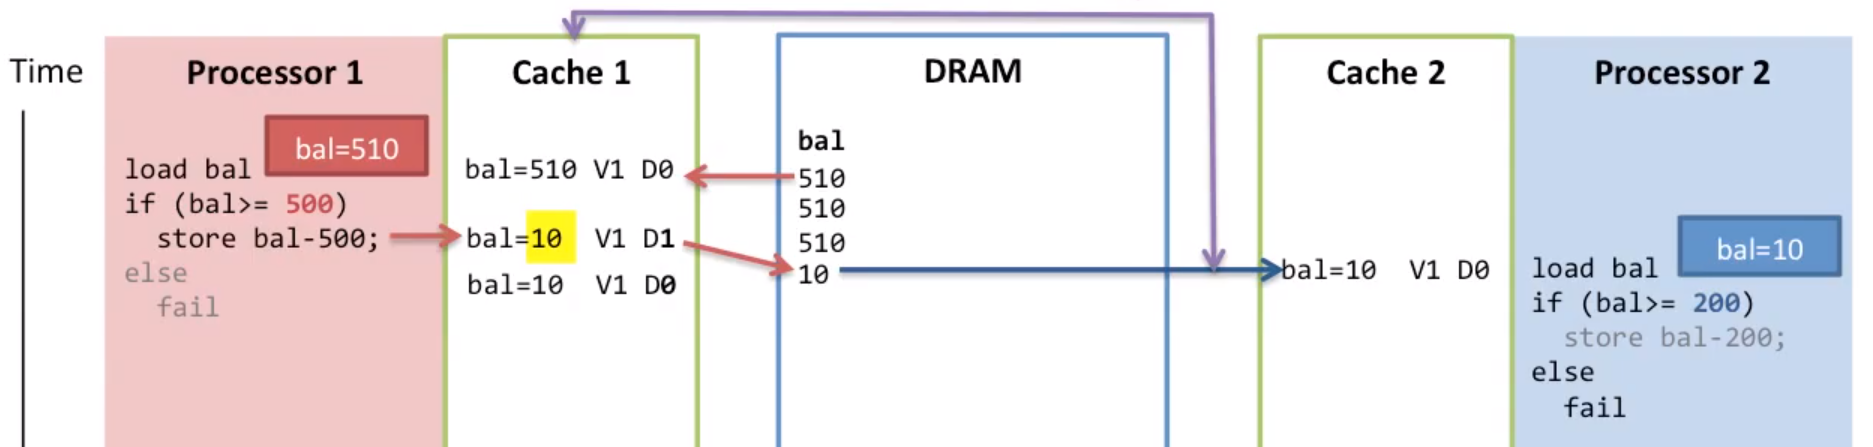
\includegraphics[width=16cm, height=5cm]{image/snooping.png}
    \caption{locks}
\end{figure}

\subsection{ILP}
\begin{itemize}
\item  Instruction level parallalism (ILP)
\item  better to have out-of-oder exicution sice we can find independent instruciions
\item  We use Dual-issue pipline so we can have one for memory instructions and
  one for non memory instruction
\item  It mrakes ISA promis with inorder exicution
\item  Issue with data hazards, more komplexity
\end{itemize}


\textbf{dual issue pipline}
\begin{figure}[h]
    \vspace{10mm}
    \centering
    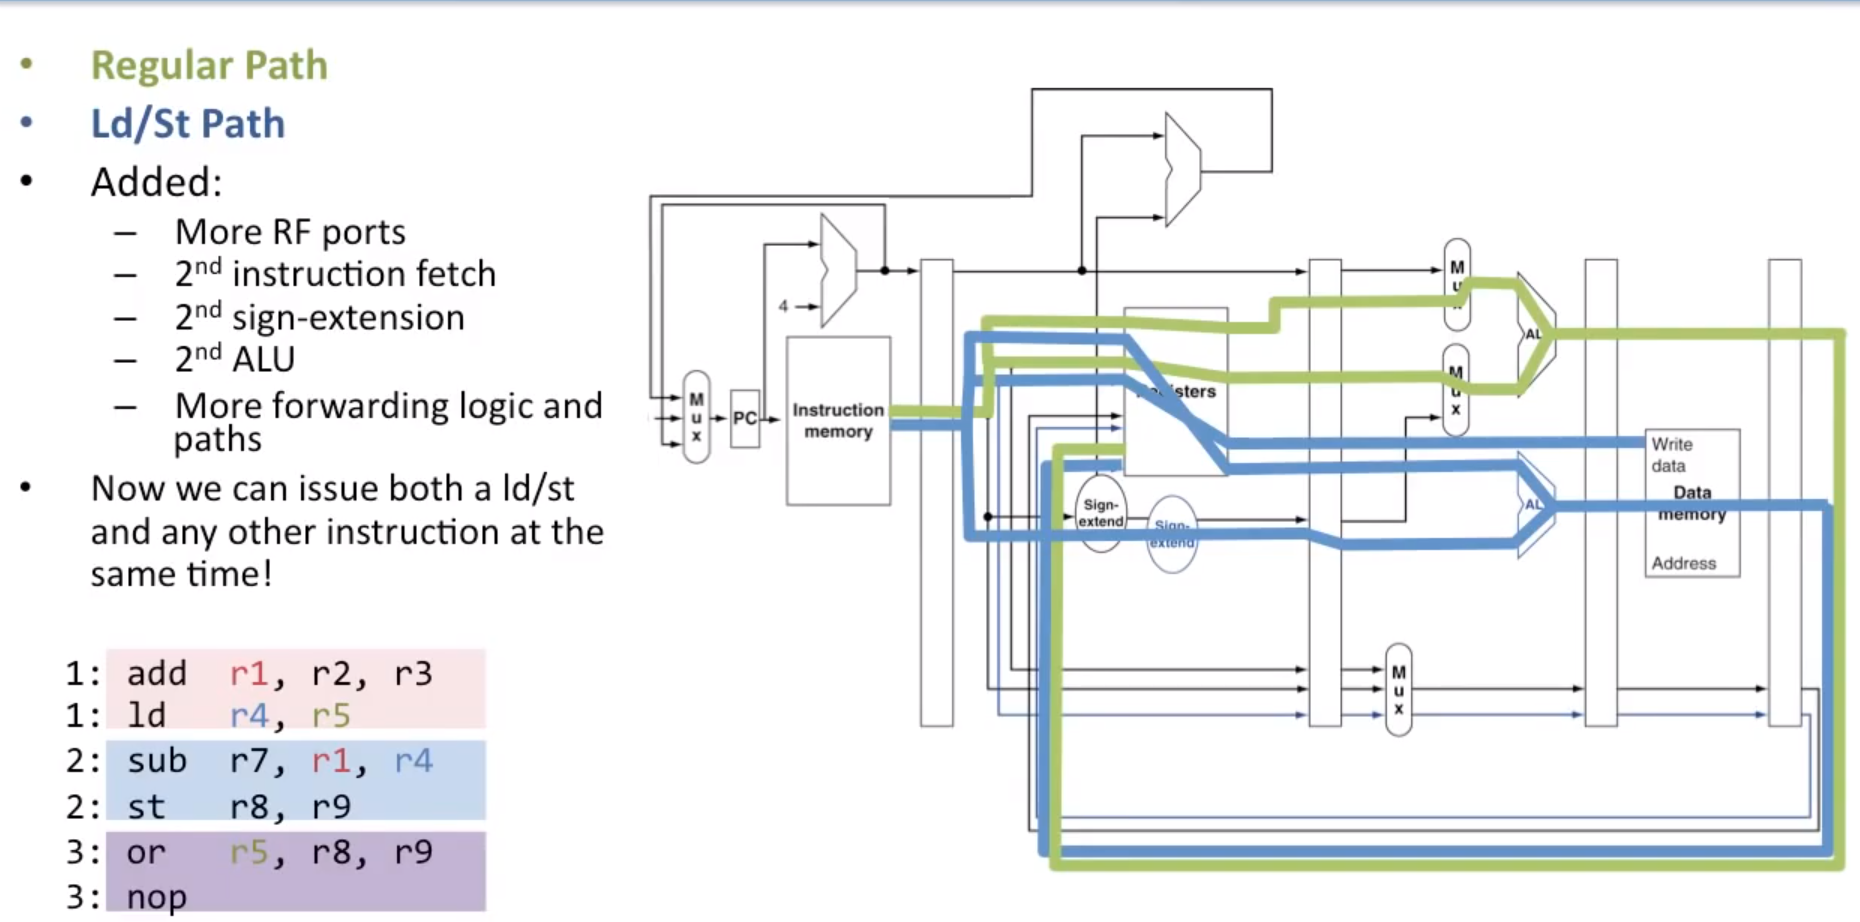
\includegraphics[width=16cm, height=7cm]{image/dual-issue-pipline.png}
    \caption{dual-issue-pipline}
\end{figure}

\textbf{Simulataneos Multithreading (SMT)}
\begin{itemize}
\item  Treads: each proscess has it own thread se it can be more easaly run in parralel
\item  SMT: allowes threads when stalled swith to another thread an run it instead  
\end{itemize}
 \newpage
\chapter{Probability and Statistics DV}

\newpage

% Resorces
% http://wrigstad.com/ioopm18/course-report2018.html
% http://wrigstad.com/ioopm19/

\section{Introduction}

\subsection{Test}
Innan: \newline
Läs igenom standard instruktionerna. \newline
Sätt upp mjukvaru miljö på skollans datorer. \newline

Under: \newline
Det är mycket tid. \newline
Läs igenom instruktionerna på uppgiften nogrant. \newline



\section{Imperative programming i C}
C is a strict programming language, we must therefore write every type of variables.
Like any other imperative programming language it execute sequentially and every argument is evaluated
in order. It also allow side effects like changing the state freely. 

\noindent\textbf{Vilkorsatser}
\begin{lstlisting}[language=C]
if (expr) { expr; } 
if (age > 100) { puts("Very old"); } 

if (expr) { expr; } else { expr; }
if (age % 2 == 0) { puts("Even"); } else { puts("Odd"); }

expr ? expr : expr
a < b ? b : a;
\end{lstlisting}

\noindent\textbf{Shortcuts loop operations}
\begin{lstlisting}[language=C]
n_fakultet *= n--;
\end{lstlisting}


\subsection{Data structurer}
\subsubsection{stack och heap}
I kortids minnet som c kompilatorn hanterar skjälv så sappar datan i en stack.
Stack funkar som talrikar som man staplar på varandra och tar den som du la senast ut.

Heap är för långtids mine och störe data som arrayer.
Det fungerar som ett rutat papper där varge ruta är en viss data size.

\noindent\textbf{Shortcuts loop operations}
För att andvända heapen, (rita på det rutade papret) måste man följa 4 steg.
\noindent\emph{ steg 1: räkna ut hur många rutor vi behöver} \newline
Använd plattformsoberoende hjälpmedel och vanlig aritmetik
\begin{lstlisting}[language=C]
  sizeof(T) * antal
  int size = sizeof(int) * 1024
\end{lstlisting}

\noindent\emph{ steg 2: reservera motsvarande yta} \newline
Här kan det gå fel — det kanske inte finns plats på papperet
\begin{lstlisting}[language=C]
  T *namn = malloc(antal bytes); 
  int *skonummer = malloc(size);
\end{lstlisting}

\noindent\emph{ steg 3: använd ytan hejvilt} \newline
Men sudda först!
(Beror på datastrukturen)

\noindent\emph{ steg 4: lämna tillbaka platsen när du är klar} \newline
Annars kommer det gå dåligt i ett framtida steg 2
\begin{lstlisting}[language=C]
  free(namn); 
  free(skonummer);
\end{lstlisting}


\subsubsection{Structar}
För att skapa egna data structurer som andvänder man sig av ``struct'' operatorn.
Om man vill gömma fler data typer i en så kan man andvända en ``union''.
För att göra en typ så andväder man ``typedef'' och avslutar med \begin{verbatim}namnet_{t}\end{verbatim}

\subsubsection{Pekare}
Pekare pekar var datan finns så man kan skicka information utan att sicka stora mängder data.

\begin{lstlisting}[language=C]
  int  a  
  int *b  
\end{lstlisting}
%// a är en variabel som innehåller ett heltal
%// b är en variabel som innehåller en adress till en plats i minnet där det finns ett heltal
Syntaxen som andvänds är:
pekartypen \begin{verbatim} int * \end{verbatim}, adresstagningsoperatorn \begin{verbatim} & \end{verbatim} och avrefereringsoperatorn \begin{verbatim} * \end{verbatim}.
  Skillnaden mellan arrayer och pointers är väldigt liten i c.
  Därför är samma oporation för string (\begin{verbatim}char *\end{verbatim})
som en pointer (\begin{verbatim} int * \end{verbatim}). Pekaren behöver inte peka på en data värde utan kan peka på flertal värden.


%https://en.wikipedia.org/wiki/C_data_types

\subsubsection{Linked list}
%https://www.youtube.com/watch?v=VOpjAHCee7c
Varge element har data av någon typ samt en pekare till nästa element.
Head and tail kan beskriva en sådan lista, då head är första ellementet
och tail är rästen.

Tid komplexiteten är: O\(n\). Linjär


\subsubsection{Hash table}
%https://www.youtube.com/watch?v=2Ti5yvumFTU&list=WL&index=5&t=686s
Hash table är ett mer effectivt sätt att hantera data istället för en array.
Då man inte behöver kålla varge element vad den finns utan andvänder en hash
function för att skapa ett ``nummer'' som pekar till vad datan finns någonstans
exempelvis kan det vara mod element i hash table då vet vi har vi ska ska söka efter.
Ett problem som kommer upstå är att data mappas till samma plats, då får man andvända
exempelvis \emph{linuer probing} som säger att om det är fult på platsen gå till nästa tills
det finns och om det inte finns så protesterar programet. Varge element inehåller inget värde
eller deleted varde om det är tomma.

Tid komplexiteten är: O\(1\). Konstant men inte i verkligheten


% F12

\section{Object-Oriented programming i Java}

%arv, amerikanska skollan ärver kåd, is skandinaviska skollan ärver betende.
%mäniska ärver från däggjur och däggjur ärver från djur, liv, ting....

%i java fiins supper klasser som man inte kan skapa en nytt dådant objekt men du andvändar classarna som extendare som du skapar.

% konstruktor är den metod som initialiserar objectet
% supper
% finnal value wont change like constant, class ej ervs
% abstarct cant creat new objects (ingen instans)

% man kan inte ha sama metod namn och argument men olika retur typer blir overload
% Tillåtet i vissa språ
kör den mest spesifica implementationen av metoden
single dispage, vi bryr os ombjectet vi kör metoden på men inte argumentet
 \newpage
\chapter{Linear Algebra and Geometry I}

\newpage

\section{Linjära ekvationssystem}

\textbf{3 gundläggande operationer för att lösa linjära ekvationer}
\begin{align*}
  &\quad (1) \text{ (Tvåpilar) Byt om på två ekvationer} \\
  &\quad (2) \text{ (Labbda) Multiplicera båda sidorna av en ekvation med } \lambda \neq 0 \\
  &\quad (3) \text{ (Labda pil) addera } \lambda
  \text{ gånga en ekvation till en annan ekvation} \\  
\end{align*}


\textbf{Generall lösning}
\begin{align*}
  &\quad  \left\{\begin{array}{l}
  a_{1} x+b_{1} y=c_{1} \\
  a_{2} x+b_{2} y=c_{2}
  \end{array}\right. \\
  &\quad  \text{Lambda pil upp}\left\{\begin{array}{l}
  a_{1} x+b_{1} y=c_{1} \\
  a_{2} x+b_{2} y=c_{2}
  \end{array}\right. \\
  &\quad  \text{Ger nya ekvationssystemet} \\
  &\quad  \text{Lambda pil upp}\left\{\begin{array}{l}
  (a_{1}+\lambda a_{2})x + (b_{1}+\lambda b_{2})y=c_{1} + \lambda c_{2} \\
  a_{2} x+b_{2} y=c_{2}
  \end{array}\right. \\
  &\quad  \text{-Lambda pil upp}\left\{\begin{array}{l}
  (a_{1}+\lambda a_{2})x + (b_{1}+\lambda b_{2})y=c_{1} + \lambda c_{2} \\
  a_{2} x+b_{2} y=c_{2}
  \end{array}\right. \\
  &\quad
\end{align*}

\textbf{Exempel linjär ekvationssystem}
\begin{align*}
  &\quad  \left\{\begin{array}{l}
  2x+3y=4 \\
  3x-y=6
  \end{array}\right. \\
  &\quad \\
  &\quad  \text{Andvänder rad operationer för att lösa ekv systemet} \\
  &\quad  (-\frac{3}{2})\text{pil ned}\left\{\begin{array}{l}
  2x+3y=4 \\
  3x-y=6
  \end{array}\right. \\
  &\quad
  (3x-y) -\frac{3}{2} (2x+3y)=6 -\frac{3}{2} \cdot 4 \Leftrightarrow{} \\
  &\quad
  (3-\frac{3}{2}\cdot 2) x + (-1 -\frac{9}{2}) y = 6 -6
  \Leftrightarrow-\frac{11}{2}y = 0 \\
  &\quad  (-\frac{2}{11})\text{ned}\left\{\begin{array}{l}
  2x+3y=4 \\
  -\frac{11}{2}y = 0
  \end{array}\right. \\
  &\quad  (-3)\text{pil upp}\left\{\begin{array}{l}
  2x+3y=4 \\
  y=0
  \end{array}\right. \\
  &\quad  (\frac{1}{2})\text{upp}\left\{\begin{array}{l}
  2x=4 \\
  y=0
  \end{array}\right. \\
  &\quad  \left\{\begin{array}{l}
  x=2 \\
  y=0
  \end{array}\right. \\
  &\quad \\
  &\quad  \text{\textbf{Kontrol:} stoppar in $x$ och $y$ i ekvationerna} \\
  &\quad  2\cdot{2}+3\cdot{0}=4 \text{ (stämmer)} \\
  &\quad  3\cdot{2}-\cdot{0}=6 \text{ (stämmer)} \\
\end{align*}


\newpage

\subsection{Total Matris}
\textbf{Termonologi}
\begin{itemize}
\item Rader och Kolonner: Rader är vågräta delen av matrisen (ekvationen)
  Kolonner är lodräta delen (koificenterna)
\item ledande ekvivalent: 
\item trappstegs matris: När ledande ekvivalent är i trapp form går ned max ett steg
\item rad kanonisk: När alla av de ledande ekvivalent inte har någon i samma kolonn
\end{itemize}

  
\textbf{Exempel matriser}
\begin{align*}
  &\quad \left\{\begin{array}{rr}
  x+2 y+ & z=-1 \\
  2 x+(a+3) y+ & 3 z=-4 \\
  x+(3-a) y+(a-2) z & =a-1
  \end{array}\right. \\
  &\quad \left(\begin{array}{ccc|c}
    1 & 2 & 1 & -1 \\
    2 & a+3 & 3 & -4 \\
    1 & 3-a & a-2 & a-1
  \end{array}\right) \\
  &\quad (-1 \text{ rad1 till rad2}), (-2 \text{ rad1 till rad3}) \\
  &\quad \left(\begin{array}{ccc|c}
    1 & 2 & 1 & -1 \\
    2 & a-1 & 1 & -2 \\
    0 & 1-a & a-3 & a
  \end{array}\right) \\
  &\quad \left(\begin{array}{ccc|c}
    1 & 2 & 1 & -1 \\
    0 & a-1 & 1 & -2 \\
    0 & 0 & a-2 & a-2
  \end{array}\right) \\
  &\quad a \neq 1 \land a \neq 2 \\
  &\quad (\frac{1}{a-2} \text{rad 3}) \\
  &\quad \left(\begin{array}{ccc|c}
    1 & 2 & 1 & -1 \\
    0 & a-1 & 1 & -2 \\
    0 & 0 & 1 & 1
  \end{array}\right) \\
  &\quad (-1 \text{rad 3 till rad 2}), (-1 \text{rad 3 till rad 1}) \\
  &\quad \left(\begin{array}{ccc|c}
    1 & 2 & 0 & -2 \\
    0 & a-1 & 0 & -3 \\
    0 & 0 & 1 & 1
  \end{array}\right) \\
  &\quad (\frac{1}{a-1} \text{rad 2}) \\
  &\quad \left(\begin{array}{ccc|c}
    1 & 2 & 0 & -2 \\
    0 & a-1 & 0 & -3 \\
    0 & 0 & 1 & 1
  \end{array}\right) \\
  &\quad \left(\begin{array}{ccc|c}
    1 & 2 & 0 & -2 \\
    0 & 1 & 0 & \frac{3}{1-a} \\
    0 & 0 & 1 & 1
  \end{array}\right) \\  
  &\quad (-2 \text{rad 2 till rad 3}) \\
  &\quad \left(\begin{array}{ccc|c}
    1 & 0 & 0 & -2 - \frac{6}{1-a} \\
    0 & 1 & 0 & \frac{3}{1-a} \\
    0 & 0 & 1 & 1
  \end{array}\right) \\  
  &\quad \left\{\begin{array}{rr}
  x & = -2 - \frac{6}{1-a} \\
  y & = \frac{3}{1-a} \\
  z & = 1
  \end{array}\right. \\
  &\quad \\
  &\quad \text{\textbf{Kontroll:} stoppar in x,y,z i ekvationerna} \\
  &\quad \left\{\begin{array}{r}
  \left(\frac{2 a-8}{1-a}\right)+\quad 2 \cdot\left(\frac{3}{1-a}\right)+\quad 1=-1 \\
  2 \cdot\left(\frac{2 a-8}{1-a}\right)+(a+3) \cdot\left(\frac{3}{1-a}\right)+\quad 3 \cdot 1=-4 \\
  \left(\frac{2 a-8}{1-a}\right)+(3-a) \cdot\left(\frac{3}{1-a}\right)+(a-2) \cdot 1=a-1
  \end{array}\right.
\end{align*}


\newpage

\section{Vektorer/koordinater i planet och rummet}
% geogebra: https://www.google.com/search?q=geogebra&source=lmns&bih=945&biw=1910&hl=en&sa=X&ved=2ahUKEwjmtZ-q9c7rAhUCxSoKHVRHCA8Q_AUoAHoECAEQAA
\textbf{Räkne regler vektorer}
\begin{align*}
  &\quad \text{A1 } \vec{u} + \vec{v} = \vec{v} + \vec{u} \\
  &\quad \text{A2 } \vec{u} + (\vec{v}+\vec{w}) = (\vec{v}+\vec{u}) + \vec{w} \\
  &\quad \text{A3 } \vec{u} + \vec{0} = \vec{u} \\
  &\quad \text{A4 } \vec{u} + \vec{v}  = \vec{0} \Leftrightarrow \vec{v} = \vec{-u} \\
  &\quad \text{M1 } 1\vec{u} = \vec{u} \\
  &\quad \text{M2 } k(l\vec{u}) = (kl)\vec{u} \\
  &\quad \text{M3 } (k+l)\vec{u} = k\vec{u} + l\vec{u} \\
  &\quad \text{M4 } k(\vec{u}+\vec{v}) = k\vec{u} + k\vec{v} \\
\end{align*}

\begin{align*}
  &\quad \vec{a} = \begin{pmatrix}
  a_1 \\
  a_2 
  \end{pmatrix} \text{ för } \mathbb{R}^2 \\
  &\quad \\
  &\quad \vec{a} = \begin{pmatrix}
  a_1 \\
  a_2 \\
  a_3
  \end{pmatrix} \text{ för } \mathbb{R}^3 \\
\end{align*}

\textbf{Definition: Parallela vektorer}
\begin{align*}
  &\quad \text{Parallela omm } \exists{k}: \vec{u} = k\vec{v} \lor k\vec{u} = \vec{v}
\end{align*}


\subsection{Bas}
Standard bas är välbikant då i planet är x och y axeln medans i ett rum är x, y och z.
Baser som inte är standard är vektorer som ej är parralella som då skappar axlar som ej
behöver vra vinkelräta. \newline

\textbf{Definition: Bas}
\begin{align*}
  &\quad  \text{Bas i plan } \forall{\vec{x}},\exists{k_1,k_2}:
  \vec{x} = k_1\vec{u} \lor k_2\vec{v} \\
  &\quad  \text{Bas generell } \vec{x} = k_1\vec{u_1}+k_2\vec{u_2}+ \ldots +k_n\vec{u_n} \\
  &\quad \underline{u}=(\vec{u_1}\vec{u_2}\ldots\vec{u_n}) \\
  &\quad
  \vec{e_1}=\begin{pmatrix}  1 \\  0 \\  0  \end{pmatrix}
  \vec{e_2}=\begin{pmatrix}  0 \\  1 \\  0  \end{pmatrix}
  \vec{e_3}=\begin{pmatrix}  0 \\  0 \\  1  \end{pmatrix} \\
\end{align*}

\textbf{Exempel: kordenatar för vektor i bas}
\begin{align*}
  &\quad \text{Låt: }
  \vec{u}=\begin{pmatrix}  2 \\  1   \end{pmatrix},
  \vec{v}=\begin{pmatrix}  -2 \\  1   \end{pmatrix} \\
  &\quad  \text{Hitta kordenarterna för vektorn }
  \vec{x}=\begin{pmatrix}  0 \\  6   \end{pmatrix} \\
  &\quad \\
  &\quad  \text{Lösning: vi måste hittar realla tal $k_1$ och $k_2$ så att } \\
  &\quad
  \begin{pmatrix}  0 \\  6   \end{pmatrix} =
  k_1\begin{pmatrix}  2 \\  1   \end{pmatrix} 
  +k_2\begin{pmatrix}  -2 \\  1   \end{pmatrix} =
  \begin{pmatrix}  2k_1-2k_2 \\  k_1+k_2   \end{pmatrix} \\
  &\quad 
  \left\{\begin{array}{r}
  2k_1-2k_2 = 0 \\
  k_1+k_2 = 6 
  \end{array}\right. \Rightarrow{}
  \begin{pmatrix}  k_1 \\  k_2   \end{pmatrix} =  \begin{pmatrix}  3 \\  3   \end{pmatrix} \\
\end{align*}


\textbf{Exempel: Om det är en bas}
\begin{align*}
  &\quad \text{För vilken värde på a är vektorerna en bas för } \mathbb{R}^3 \\
  &\quad
  \vec{u_1} = \begin{pmatrix}  1 \\  2 \\  3  \end{pmatrix},
  \vec{u_2} = \begin{pmatrix}  1 \\  2 \\  a  \end{pmatrix},
  \vec{u_3} = \begin{pmatrix}  1 \\  a \\  3  \end{pmatrix} \\
  &\quad \\
  &\quad  \text{Vi måste hitta ett a sådant att} \\
  &\quad  k_1\begin{pmatrix}  1 \\  2 \\  3  \end{pmatrix},
  k_2\begin{pmatrix}  1 \\  2 \\  a  \end{pmatrix},  k_3\begin{pmatrix}  1 \\  a \\  3
  \end{pmatrix} =  \begin{pmatrix} ? \\  ? \\  ?  \end{pmatrix} \\
  &\quad
  \begin{gmatrix}[p]
    1 & 1 & 1 \\
    2 & 2 & a \\
    3 & a & 3
    \rowops
    \add[-2]{0}{1}
    \add[-3]{0}{2}
  \end{gmatrix} \sim 
  \begin{gmatrix}[p]
    1 & 1 & 1 \\
    0 & 0 & (a-2) \\
    0 & (a-3) & 0
  \end{gmatrix} \\
  &\quad \text{Om a = 2: då är sista ekvationen 0 =? och vi ser att lösningarna får parametrar} \\
  &\quad \text{och därför: antingen ingen lösningar eller oändligt många lösningar.} \\
  &\quad \text{Oavsett -ej bas} \\
  &\quad \text{Om a = 3: då blir det samma problem som a=2} \\
  &\quad \\
  &\quad \text{Svar: de tre vektorer är en basa om a inte är 2 eller 3} \\
\end{align*}


\textbf{Definition: Punkter i planet}
\begin{align*}
  &\quad  \text{Från origo: alla } P=(x,y) \text{ och }
  \overrightarrow{OP} = \begin{pmatrix}  x \\  y   \end{pmatrix} \\
  &\quad  \text{Om } A=(a_1,a_2) \text{ och } B=(b_1,b_2) \text{ då är }
  \overrightarrow{AB} =  \begin{pmatrix}  b_1-a_1 \\  b_2-a_2   \end{pmatrix} \\
\end{align*}


\textbf{Definition: Längd}
\begin{align*}
  &\quad  \text{Längd vektor i plan } |\vec{v}| = \sqrt{a^2+b^2} \\
  &\quad  \text{Längd vektor i rum } |\vec{v}| = \sqrt{a^2+b^2+c^2} \\
\end{align*}


\newpage

\section{Skalärprodukt och vektorprodukt}
\subsection{Skalärprodukt}
\begin{align*}
  &\quad  \vec{u}\bullet\vec{v} = |\vec{u}||\vec{v}|\cos{\theta} \\
  &\quad  \vec{u}\bullet\vec{v} = u_1v_1+u_2v_2+ \ldots +u_3v_3 \\
\end{align*}

\textbf{Räkneregler}
\begin{align*}
  &\quad  \vec{u}\bullet\vec{v} = \vec{v}\bullet\vec{u} \\
  &\quad  \vec{u}\bullet(\vec{v}+\vec{w}) = \vec{u}\bullet\vec{v} + \vec{u}\bullet\vec{w} \\
  &\quad  \lambda(\vec{u}\bullet\vec{v}) = (\lambda\vec{u})\bullet\vec{v} =
  \vec{u}\bullet(\lambda\vec{v}) \\
  &\quad  \vec{u}\bullet\vec{u} = |\vec{v}|^2 \\
  &\quad  \vec{u}\bullet\vec{u} = 0 \Leftrightarrow \vec{u} = \vec{0} \\
\end{align*}

\textbf{Exempel: parrallel och ortogonal}
\begin{align*}
  &\quad  \text{För vilka värden på a och b är vektorerna i } \mathbb{R}^3
  \begin{pmatrix}  1 \\  a \\  2  \end{pmatrix} \text{ och }
  \begin{pmatrix}  b \\  8 \\  a  \end{pmatrix} \\
  &\quad  \text{ (a) parallel?, (b) ortognala?}  \\
  &\quad  \\
  &\quad  (a) \\
  &\quad
  \left\{\begin{array}{r}
  k = b \\
  ak = 8 \\
  2k = a
  \end{array}\right.  \Rightarrow{} \\
  &\quad
  \left\{\begin{array}{r}
  k = b \\
  (2k)k = 8  \Rightarrow{} k^2 = 4  \Rightarrow{} k = 2  \\ 
  2k = a
  \end{array}\right. \\
  &\quad  k=b=2, a=4 \\
  &\quad (b) \\
  &\quad
  \begin{pmatrix}  1 \\  a \\  2  \end{pmatrix} \bullet{}
  \begin{pmatrix}  b \\  8 \\  a  \end{pmatrix} = 1b+a2+2a = b+4a = 0 \\
\end{align*}


\textbf{Exempel: Längd-formeln}
\begin{align*}
  &\quad  |\vec{v}| = \sqrt{|\vec{v}|^2} = \sqrt{|\vec{v}|\bullet|\vec{v}|}  \\
  &\quad  \text{Beräkna längden av (ON-bas): } 
  \vec{v} = \begin{pmatrix} 2 \\ 1 \\ 2 \end{pmatrix} \\
  &\quad
  \begin{pmatrix} 2 \\ 1 \\ 2 \end{pmatrix} \bullet \begin{pmatrix} 2 \\ 1 \\ 2 \end{pmatrix} =
  2^2 + 1^2 + 2^2 = 9 \Rightarrow \\
  &\quad  |\vec{v}| = \sqrt{9} = 3 \\
  &\quad  \text{Därmed är längden: } 3 \\
\end{align*}


\textbf{Exempel: Vinkel-formeln}
\begin{align*}
  &\quad  \text{Låt $\vec{u}$ och $\vec{v}$ vara vektorer och vinkel blir då: } \\
  &\quad  \theta = \arccos{\frac{\vec{u}\bullet\vec{v}}{|\vec{u}||\vec{v}|}} \\
  &\quad  \text{Beräkna vinkeln av (ON-bas): } 
  \vec{u} = \begin{pmatrix} 1 \\ 2 \\ 2 \end{pmatrix} 
  \text{ och }
  \vec{v} = \begin{pmatrix} 2 \\ 2 \\ 1 \end{pmatrix} \\
  &\quad
  \begin{pmatrix} 1 \\ 2 \\ 2 \end{pmatrix} \bullet \begin{pmatrix} 2 \\ 2 \\ 1 \end{pmatrix} =
  1\cdot{2} + 2^2 + 2\cdot{1} = 8 \\
  &\quad  |\vec{u}| = \sqrt{1^2+2^2+2^2}=\sqrt{9}=3 \\
  &\quad  |\vec{v}| = \sqrt{2^2+2^2+1^2}=\sqrt{9}=3 \\
  &\quad \arccos{\frac{\vec{u}\bullet\vec{v}}{|\vec{u}||\vec{v}|}} =
  \arccos{\frac{8}{3\cdot{3}}} = \arccos{\frac{8}{9}} \approx 27.27^\circ
\end{align*}


\textbf{Exempel: Längd av två vektorer}
\begin{align*}
  &\quad  \text{Låt u och v vara två vektorer sådana att} \\
  &\quad  |\vec{u}|=4, |\vec{v}|=2 \text{ och vinkeln mellan $\vec{u}$ och $\vec{v}$ är } \frac{2\pi}{3} \\
  &\quad  \text{Bestäm längden av } 3\vec{u}-2\vec{v} \\
  &\quad  \\
  &\quad  \sqrt{|3\vec{u}-2\vec{v}|^2} =
  \sqrt{ 9|\vec{u}|^2 + 4|\vec{v}|^2 - 2|\vec{u}||\vec{v}|\cos{\frac{2\pi}{3}}}  \\
  &\quad  \sqrt{9\cdot{}16 + 4\cdot{}4 - 4\cdot{}3\cdot{}8\cdot{\frac{-1}{2}} } =
  \sqrt{13\cdot{}16} = 4\sqrt{13} \\
\end{align*}

\textbf{Exempel: beräkna skalärprudukten}
\begin{align*}
  &\quad  \underline{u}\begin{pmatrix} 9 \\ 9 \end{pmatrix} \bullet
  \underline{u}\begin{pmatrix} -2 \\ -1 \end{pmatrix} \\
  &\quad  \underline{u}=(\vec{u_1},\vec{u_2}), \, \vec{u_1}\bullet\vec{u_1}=9, \,
  \vec{u_1}\bullet\vec{u_2}=6, \, \vec{u_2}\bullet\vec{u_2}=8 \\
  &\quad  \\
  &\quad  \underline{u}\begin{pmatrix} 9 \\ 9 \end{pmatrix} \bullet
  \underline{u}\begin{pmatrix} -2 \\ -1 \end{pmatrix} =
  (9\vec{u_1}-2\vec{u_2})\bullet(9\vec{u_1}-1\vec{u_2}) =
  -18|\vec{u_1}|^2+(-9-18)\vec{u_1}\bullet\vec{u_1}-9|\vec{u_2}|^2 \\
  &\quad = -18\cdot{9}-27\cdot(6)-9\cdot{8} =-396
\end{align*}


\newpage

\subsection{Ortogonal projektion}
Hitta punkt på linjen som är närmast en punkt. Punkten är ortogonala (vinkelrätta) \newline
Parralell koposant skrivs $\vec{v}_{||{l}}$ och ortogonal skrivs $\vec{v}_{\perp{l}}$.

\begin{figure}[h]
    \vspace{10mm}
    \centering
    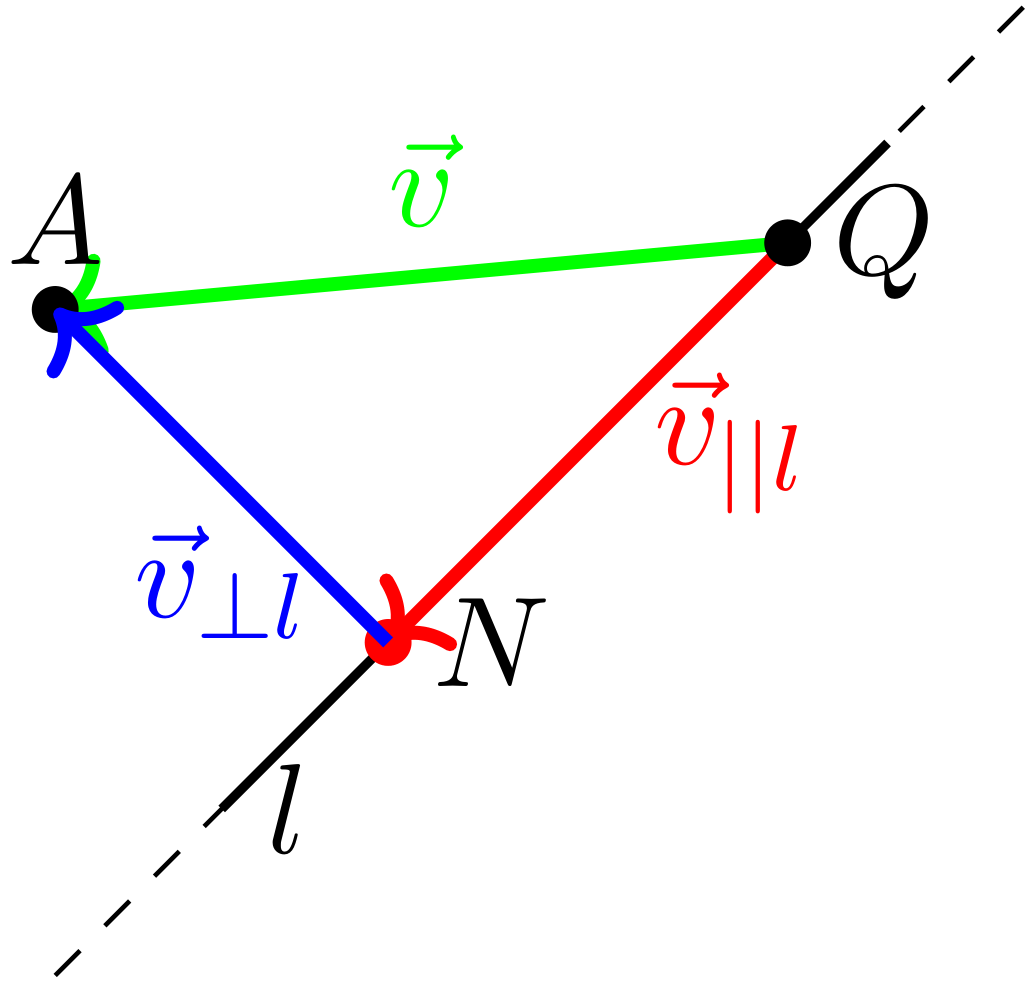
\includegraphics[width=5cm, height=5cm]{image/Ortogonal-projektion.png} 
    \caption{Ortogonal projektion}
\end{figure}

\textbf{Ortogonal projektion Formeln}
\begin{align*} 
  &\quad  \vec{v}_{||{l}} = \frac{\vec{u}\bullet{\vec{v}}}{|\vec{u}|^2}\vec{u}  \\
\end{align*}
%  &\quad  \vec{v}_{\perp{l}} = \vec{v}-\vec{v}_{||l} = \vec{v}-k\vec{u} \\

\textbf{Exempel: Hitta parralel och ortogonal komposanten}
\begin{align*} 
  &\quad  \vec{v} = \vec{v}_{\perp{l}} + \vec{v}_{||{l}} \\
  &\quad  \vec{v}_{||{l}} = \frac{\vec{u}\bullet{\vec{v}}}{|\vec{u}|^2}\vec{u}  \\
  &\quad  \text{Beräkna ortogonal komposanten av: } \\
  &\quad
  \vec{v} = \begin{pmatrix} 1 \\ -2 \\ 3 \end{pmatrix} \text{ och }
  \vec{u} = \begin{pmatrix} -4 \\ 4 \\ 2 \end{pmatrix} \\
  &\quad  \text{Beräkna först parrallel komposanten: } \\
  &\quad  \vec{v}_{||{\vec{u}}} = \frac{\vec{u}\bullet{\vec{v}}}{|\vec{u}|^2}\vec{u} = \frac{-18}{36}\vec{u}
  = \begin{pmatrix} 2 \\ -2 \\ 1 \end{pmatrix} \\
  &\quad  \text{Ortogonal komposanten blir då: } \\
  &\quad  \vec{v}_{\perp{\vec{u}}} = \vec{v} - \vec{v}_{||{\vec{u}}}
  = \begin{pmatrix} 1-2 \\ -2+2 \\ 3-1 \end{pmatrix} \\
  &\quad  \text{Svar: } \begin{pmatrix} -1 \\ 0 \\ 2 \end{pmatrix}
\end{align*}

%exempel hitta punkt
\textbf{Exempel: Närmaste punkt och avståndet}
\begin{align*} 
  &\quad  \text{Bestäm avståndet från punkten $P=(-2,4,3)$ till linjen } \\
  &\quad  \left\{\begin{array}{r}
  x+2y-z=1 \\
  x-y+5z=4 
  \end{array}\right. \\  
  &\quad  \text{Finn även den punkt på linjen l som ligger närmast punkten P}  \\
  &\quad  \\
  &\quad  \text{Skriver ekvationen på parameter form } \\
  &\quad
  \begin{gmatrix}[p]
    1 & 2  & -1 & | & 1 \\
    1 & -1 &  5 & | & 4
    \rowops{
      \add[-1]{0}{1}}
      \mult{1}{\cdot 1/3}
  \end{gmatrix} \sim{}
  \begin{gmatrix}[p]
    1 & 2  & -1 & | & 1 \\
    0 & 1 &  -2 & | & -1
    \rowops{
    \add[-2]{1}{0}}
  \end{gmatrix} \sim{}  \\
  &\quad
  \begin{gmatrix}[p]
    1 & 0  &  3 & | & 3 \\
    0 & 1 &  -2 & | & -1
    \rowops{
    \add[-1]{0}{1}}
  \end{gmatrix} \sim{}  \\
  &\quad   l:\begin{pmatrix} x \\ y \\ z \end{pmatrix} =
  \begin{pmatrix} 3 \\ -1 \\ 0 \end{pmatrix}+
  t\begin{pmatrix} -3 \\ 2 \\ 1 \end{pmatrix}  \, \text{ dvs } (p_0 + t\vec{v})\\
  &\quad  \text{Hittar en godtycklig punkt ex } t=1 \Rightarrow{}
  Q=\begin{pmatrix} 0 \\ 1 \\ 1 \end{pmatrix}  \\
  &\quad \\
  &\quad  \text{(1.) beräknar vektorn från godtykliga punkten till den givna } \\
  &\quad  \overrightarrow{PQ}=
  \begin{pmatrix} 0-(-2) \\ 1 -4 \\ 1-3 \end{pmatrix} =
  \begin{pmatrix} 2 \\ -3 \\ -2 \end{pmatrix} \\
  &\quad  \text{(2.) Beräknar ortogonala projectionen } \\
  &\quad  \overrightarrow{NQ}=\overrightarrow{PQ}_{||v}=
  \frac{\begin{pmatrix} 2 \\ -3 \\ -2 \end{pmatrix}\bullet{}
    \begin{pmatrix} -3 \\ 2 \\ 1 \end{pmatrix}}{9+4+1}
  \begin{pmatrix} -3 \\ 2 \\ 1 \end{pmatrix} =
  \frac{-14}{14}\begin{pmatrix} -3 \\ 2 \\ 1 \end{pmatrix} \\
  &\quad  \text{(3.) Beräknar punkten från närmaste punkt till } \\
  &\quad  \overrightarrow{ON}=\overrightarrow{OQ}+\overrightarrow{QN}=
  \overrightarrow{OQ}-\overrightarrow{NQ}=
  \begin{pmatrix} 0 \\ 1 \\ 1 \end{pmatrix}+
  \begin{pmatrix} -3 \\ 2 \\ 1 \end{pmatrix}=
  \begin{pmatrix} -3 \\ 3 \\ 2 \end{pmatrix} \\
  &\quad  \text{(4.) Beräknar längden }
  |\begin{pmatrix} -2 \\ 4 \\ 3 \end{pmatrix}-\begin{pmatrix} -3 \\ 3 \\ 2 \end{pmatrix}|
  =\sqrt{1^2+1^2+1^2}=\sqrt{3} \\
  &\quad  \\
  &\quad  \text{Svar: avståndet är $\sqrt{3}$ och punten är $(-3,3,2)$} \\
\end{align*}

\textbf{Exempel: Spegling}
\begin{align*} 
  &\quad  \text{Bestäm speglingen av punkten $A:(1,3,-3)$ i planet } \pi \\
  &\quad  \text{som går genom origo och innehåller punkterna}  \\
  &\quad  (-1,1,1) \text{ och } (3,3,1) \\
  &\quad  \\
  &\quad  \text{Beräknar planets ekvation} \\
  &\quad
  \vec{n}=\overrightarrow{OQ}\times\overrightarrow{OP}=
  \begin{pmatrix} -1 \\ 1 \\ 1 \end{pmatrix}\times
  \begin{pmatrix} 3 \\ 3 \\ 1 \end{pmatrix} =
  \begin{pmatrix} -2 \\ 4 \\ 6 \end{pmatrix} =
  2\begin{pmatrix} -1 \\ 2 \\ 3 \end{pmatrix} \\
  &\quad  -x+2y+3z=0 \text{ Eftersom den går egenom origo} \\
  &\quad  \overrightarrow{NA}=\overrightarrow{OA}_{||\vec{n}}=
  \frac{\begin{pmatrix} 1 \\ 3 \\ -3 \end{pmatrix}\times
    \begin{pmatrix} -1 \\ 2 \\ 3 \end{pmatrix}}{1+4+9}
  \begin{pmatrix} -1 \\ 2 \\ 3 \end{pmatrix}=
  \frac{14}{14}\begin{pmatrix} -1 \\ 2 \\ -3 \end{pmatrix} =
  \begin{pmatrix} -1 \\ 2 \\ -3 \end{pmatrix} \\
  &\quad  \text{Beräkna speglingen rita då är det upenbart } \\
  &\quad  \overrightarrow{OA'}= \overrightarrow{OA}-2\overrightarrow{NA}=
  \begin{pmatrix} 1 \\ 2 \\ -3 \end{pmatrix}-
  2\begin{pmatrix} -1 \\ 2 \\ -3 \end{pmatrix}=
  \begin{pmatrix} 3 \\ 1 \\ 3 \end{pmatrix} \\
\end{align*}


\textbf{Exempel Hitta punkt ortogonal projektion} % ex5 s12 f06
\begin{align*} 
  &\quad  \text{Låt $l$ vara linjen genom punkten $Q=(1,2,3)$ parallell med vektorn} \\
  &\quad  \vec{u} =
  \begin{pmatrix}  3 \\  4 \\  5  \end{pmatrix} \\
  &\quad  \text{Hitta den punkt $N$ på $l$ som är närmast } A=(1,7,4) \\
  &\quad  \\
  &\quad  \text{Lösning: Rita figur och tolka. Vi ortogonalt projeicerar} \\
  &\quad  \vec{v} = \overrightarrow{QA} =
  \begin{pmatrix}  1-1 \\  7-2 \\  4-3  \end{pmatrix} =
  \begin{pmatrix}  0 \\  5 \\ 1  \end{pmatrix} \text{ på vektorn }  \vec{u} \\
  &\quad \vec{v}_{||l} = \vec{v}_{||\vec{u}} = \frac{
    \begin{pmatrix} 3 \\ 4 \\ 5 \end{pmatrix} \bullet \begin{pmatrix} 0 \\ 5 \\ 1 \end{pmatrix}}{
    \begin{pmatrix} 3 \\ 4 \\ 5 \end{pmatrix} \bullet \begin{pmatrix} 3 \\ 4 \\ 5 \end{pmatrix}}
  \begin{pmatrix} 3 \\ 4 \\ 5 \end{pmatrix}
  = \frac{25}{50}\begin{pmatrix} 3 \\ 4 \\ 5 \end{pmatrix} \\
  &\quad  \text{Detta är ju igen vektorn som pekar frpn $Q$ till närmaste punkten som därför blir} \\
  &\quad  N = \Big( 1-\frac{1}{2}3, 2-\frac{1}{2}4, 3-\frac{1}{2}5 \Big)
  = \Big( -\frac{1}{2},0,\frac{1}{2} \Big) \\
  &\quad  \\
  &\quad  \text{\textbf{Kontroll:} kollar om } \overrightarrow{NQ} = k\vec{u}, \, k\in\mathbb{R} \\
  &\quad  \begin{pmatrix} 1-(-1/2) \\ 2-0 \\ 3-1/2 \end{pmatrix} =
  \begin{pmatrix} 3/2 \\ 2 \\ 5/2 \end{pmatrix} =
  \frac{1}{2}\begin{pmatrix} 3 \\ 4 \\ 5 \end{pmatrix} \text{(stämmer)} \\
\end{align*}


\textbf{Räkneregler ortogonal}
\begin{align*} 
  &\quad  \text{För vektorer $\vec{u}$, $\vec{v}$ och $\vec{w}$ och skalär $\lambda\in\mathbb{R}$} \\
  &\quad  {(\lambda\vec{v})}_{||\vec{u}}=\lambda(\vec{v}_{||\vec{u}}) \\
  &\quad  {(\vec{v}+\vec{w})}_{||\vec{u}} = \vec{v}_{||\vec{u}} + \vec{v}_{||\vec{u}} \\
  &\quad  {(\lambda\vec{v})}_{\perp{\vec{u}}} = \lambda(\vec{v}_{\perp\vec{u}}) \\
  &\quad  {(\vec{v}+\vec{w})}_{\perp{\vec{u}}} = \vec{v}_{\perp{\vec{u}}} + \vec{v}_{\perp{\vec{u}}} \\
\end{align*}


\newpage

\subsection{Enhetsvektorer och ON-baser}
\begin{align*} 
  &\quad  \text{En enhetsvektor är en vektor med längd 1.} \\
  &\quad  \text{Om man har en vektor $\vec{u}$ kan man skala om
    den med ett positivt tal så den får längd 1.} \\
  &\quad  \text{En bas } \underline{\vec{u}} = (\vec{u_1} \vec{u_2} \ldots \vec{u_n})
  \text{kallas en ortonormal bas (ON-bas) omm:} \\
  &\quad  \text{(1)  Alla vektorerna är enhetsvektorer }
  |\vec{u_1}|^2 = \vec{u_i}\bullet\vec{u_j} = 1 \\
  &\quad  \text{(2)  Varje par av vektorer $\vec{u_i}$ och $\vec{u_j}$ for $i\neq{j}$ är ortogonala:}
  \vec{u_i}\bullet\vec{u_j}=0 \\
  &\quad  \hat{\vec{u}} = \frac{1}{|\vec{u}|}\vec{u} \\
\end{align*}

Skalärproducten har samma räkneregler i ON-baser som i standard bas


\subsection{Vektorprodukten}
% https://www.youtube.com/watch?v=0GcuwYlV2ng&t=470s
I högersystem kan representeras av en höger hand där tumen är vektorn 1 pekfingret är 2
och långfingret är 3.
%bild
\textbf{Definition: högersystem}
\begin{align*} 
  &\quad  \text{En bas $\underline{u} = (\vec{u}_1 \vec{u}_2 \vec{u}_3)$
    kallas ett högersystem omm: } \\
  &\quad  \text{set ifrån spetsen av $\vec{u}_3$ vridas $\vec{u}_1$ moturs till $\vec{u}_2$} \\
\end{align*}

\textbf{Definition: Vektorprodukten}
\begin{align*} 
  &\quad  \text{Givet två icke-parallella vektorer $\vec{u}$ och $\vec{u}$ med vinkel $\theta$} \\
  &\quad  \text{mellan dem definieras $\vec{u}\times\vec{v}$ som den entydiga vektor som uppfyller} \\
  &\quad  \text{(a) } \vec{u}\times\vec{v} \text{ är ortogonal mot båda $\vec{u}$ och $\vec{v}$}  \\
  &\quad  \text{(b) längden av } \vec{u}\times\vec{v} \text{ är } |\vec{u}\vec{v}\sin{\theta}| \\
  &\quad  \text{(c) } (\vec{u} \vec{v} \vec{u}\times\vec{v}) \text{ är ett högersystem} \\
  &\quad  \text{I fallet där $\vec{u}$ och $\vec{v}$ är parallella är }
  \vec{u}\times\vec{v}=\vec{0} \\
\end{align*}

\textbf{Definition: produkter}
\begin{align*} 
  &\quad  \text{Sala om: tal $\cdot$ vektor = vektor} \\
  &\quad  \text{Skalär produkt: vektor $\bullet$ vektor = tal} \\
  &\quad  \text{Vektor produkt: vektor $\times$ vektor = vektor} \\
\end{align*}

\textbf{Räkneregler: Vektorprodukten }
\begin{align*} 
  &\quad  \text{För vektorer $\vec{u},\vec{v},\vec{w}$ och ett tal $\lambda$ gäller} \\
  &\quad  \vec{u}\times\vec{v}=-\vec{v}\times\vec{u} \\
  &\quad  \vec{u}\times(\vec{v}+\vec{w}) = \vec{u}\times\vec{v}+\vec{u}\times\vec{w}  \\
  &\quad  \lambda(\vec{u}\times\vec{v}) = \lambda(\vec{u})\times\vec{v}
  = \vec{u}\times(\lambda\vec{v}) \\
\end{align*}

\newpage
\textbf{Vektorprodukten metologi}
\begin{figure}[h]
    \vspace{10mm}
    \centering
    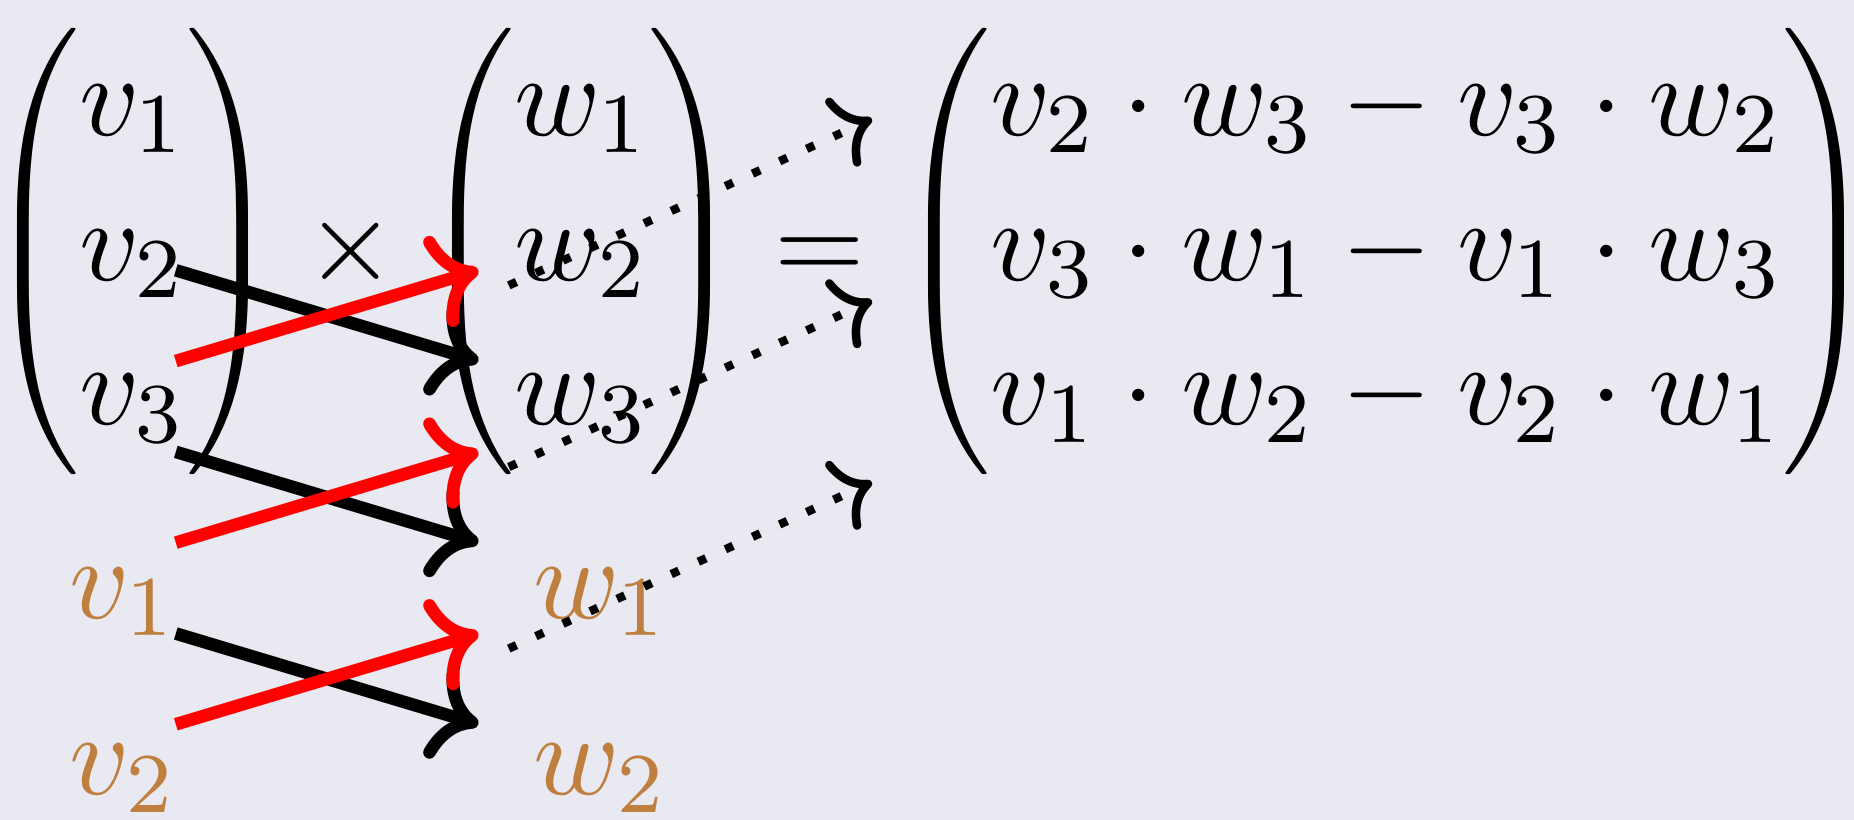
\includegraphics[width=12cm, height=5cm]{image/vektorprodukt.png} 
    \caption{Vektorprodukten}
\end{figure}

\textbf{Exempel: Hitta basen}
\begin{align*} 
  &\quad  \text{Låt }
  \vec{u}_1 = \begin{pmatrix} 4 \\ 8 \\ 1 \end{pmatrix} \text{ och }
  \vec{u}_2 = \begin{pmatrix} 4 \\ -1 \\ -8 \end{pmatrix} \\
  &\quad  \text{Verifiera att dessa är ortogonala, och hitta en vektor } \vec{u}_3 \\
  &\quad  \text{Så att } \underline{u} = (\hat\vec{u}_1 \hat\vec{u}_2 \hat\vec{u}_3)
  \text{ är en ON-bas (och skriv ut denna)} \\
  &\quad  \\
  &\quad  \text{Lösning: Först kollar vi att skalärprodukten är } 0: \\
  &\quad
  \begin{pmatrix} 4 \\ 8 \\ 1 \end{pmatrix} \bullet \begin{pmatrix} 4 \\ -1 \\ -8 \end{pmatrix}
  = 16-8-8=0 \\
  &\quad  \text{Där med ortogonala. Nu måste vi hitta en vektor som är ortogonal mot båda } \\
  &\quad  \text{vektorprodukten är just det } \\
  &\quad  \vec{u}_3 =
  \begin{pmatrix} 4 \\ 8 \\ 1 \end{pmatrix} \times \begin{pmatrix} 4 \\ -1 \\ -8 \end{pmatrix}
  \begin{pmatrix} -64+1 \\ 4+32 \\ -4-32 \end{pmatrix} =
  \begin{pmatrix} -63 \\ 36 \\ -36 \end{pmatrix} \\
  &\quad  \text{Längderna av dessa är (råkar vara lika)}  \\
  &\quad  |\vec{u}_2|^2 = |\vec{u}_1|^2 = 4^2 + {(\pm{8})}^2 + {(\pm{1})}^2 = 81 \\
  &\quad  \text{och vi kunna göra liknade beräkning för } \vec{u}_3 \text{, men vi vet redan att:} \\
  &\quad  |\vec{u}_3| = |\vec{u}_1||\vec{u}_2|\sin{\theta}=9\cdot{}9\cdot{}1=81 \\
  &\quad  \text{Desras tre normering blir därför:} \\
  &\quad  \hat\vec{u}_1 = \frac{1}{9}\begin{pmatrix} 4 \\ 8 \\ 1 \end{pmatrix},
  \hat\vec{u}_2 = \frac{1}{9}\begin{pmatrix} 4 \\ -1 \\ -8 \end{pmatrix}
  \hat\vec{u}_1 = \frac{1}{81}\begin{pmatrix} -63 \\ 36 \\ -36 \end{pmatrix}=
  \frac{1}{9}\begin{pmatrix} -7 \\ 4 \\ -4 \end{pmatrix} \\
  &\quad  \text{Så basen är: }
  \underline{u} = \Bigg(
  \frac{1}{9}\begin{pmatrix} 4 \\ 8 \\ 1 \end{pmatrix},
  \frac{1}{9}\begin{pmatrix} 4 \\ -1 \\ -8 \end{pmatrix},
  \frac{1}{81}\begin{pmatrix} -63 \\ 36 \\ -36 \end{pmatrix}
  \Bigg) \\
\end{align*}

\textbf{Exempel: Uttryck vektorer i varandra (2.5.8.b)}
\begin{align*}
  &\quad  \text{Uttryck $w$ i $u$ och $v$} \\
  &\quad  |u|=6, \, |v|=8, |w|=7, \text{ $u$ och $v$ bildar vinkeln } \frac{\pi}{6}, \\
  &\quad  \text{ $u$ och $w$ vinkeln } \frac{\pi}{2} \text{ och $v$ och $w$ vinkeln } 
  \frac{2\pi}{3}  \\
  &\quad  \\
  &\quad  \text{Altså ska hitta } \vec{w}=k_1\vec{u}+k_2\vec{v}, \, k_1,k_2\in\mathbb{R} \\
  &\quad  \text{Vi ser att $k_2<0$ enlight bild, därmed får vi följande } \\
  &\quad  -k_2\cdot\cos{\frac{\pi}{3}}=7 \Rightarrow -k_2\cdot{\frac{1}{2}}\cdot{8}=7
  \Rightarrow k_2=\frac{7}{4} \\
  &\quad  \text{Beräknarn $k_1$ } \\
  &\quad  6k_1=\frac{7}{4}\cdot{8}\cdot{\sin{\frac{\pi}{3}}} \Rightarrow k_1=\frac{7}{6}\sqrt{3} \\
  &\quad  \vec{w}=\frac{7\sqrt{3}}{6}\vec{u}-\frac{7}{4}\vec{v} \\
\end{align*}
\begin{figure}[h]
    \vspace{10mm}
    \centering
    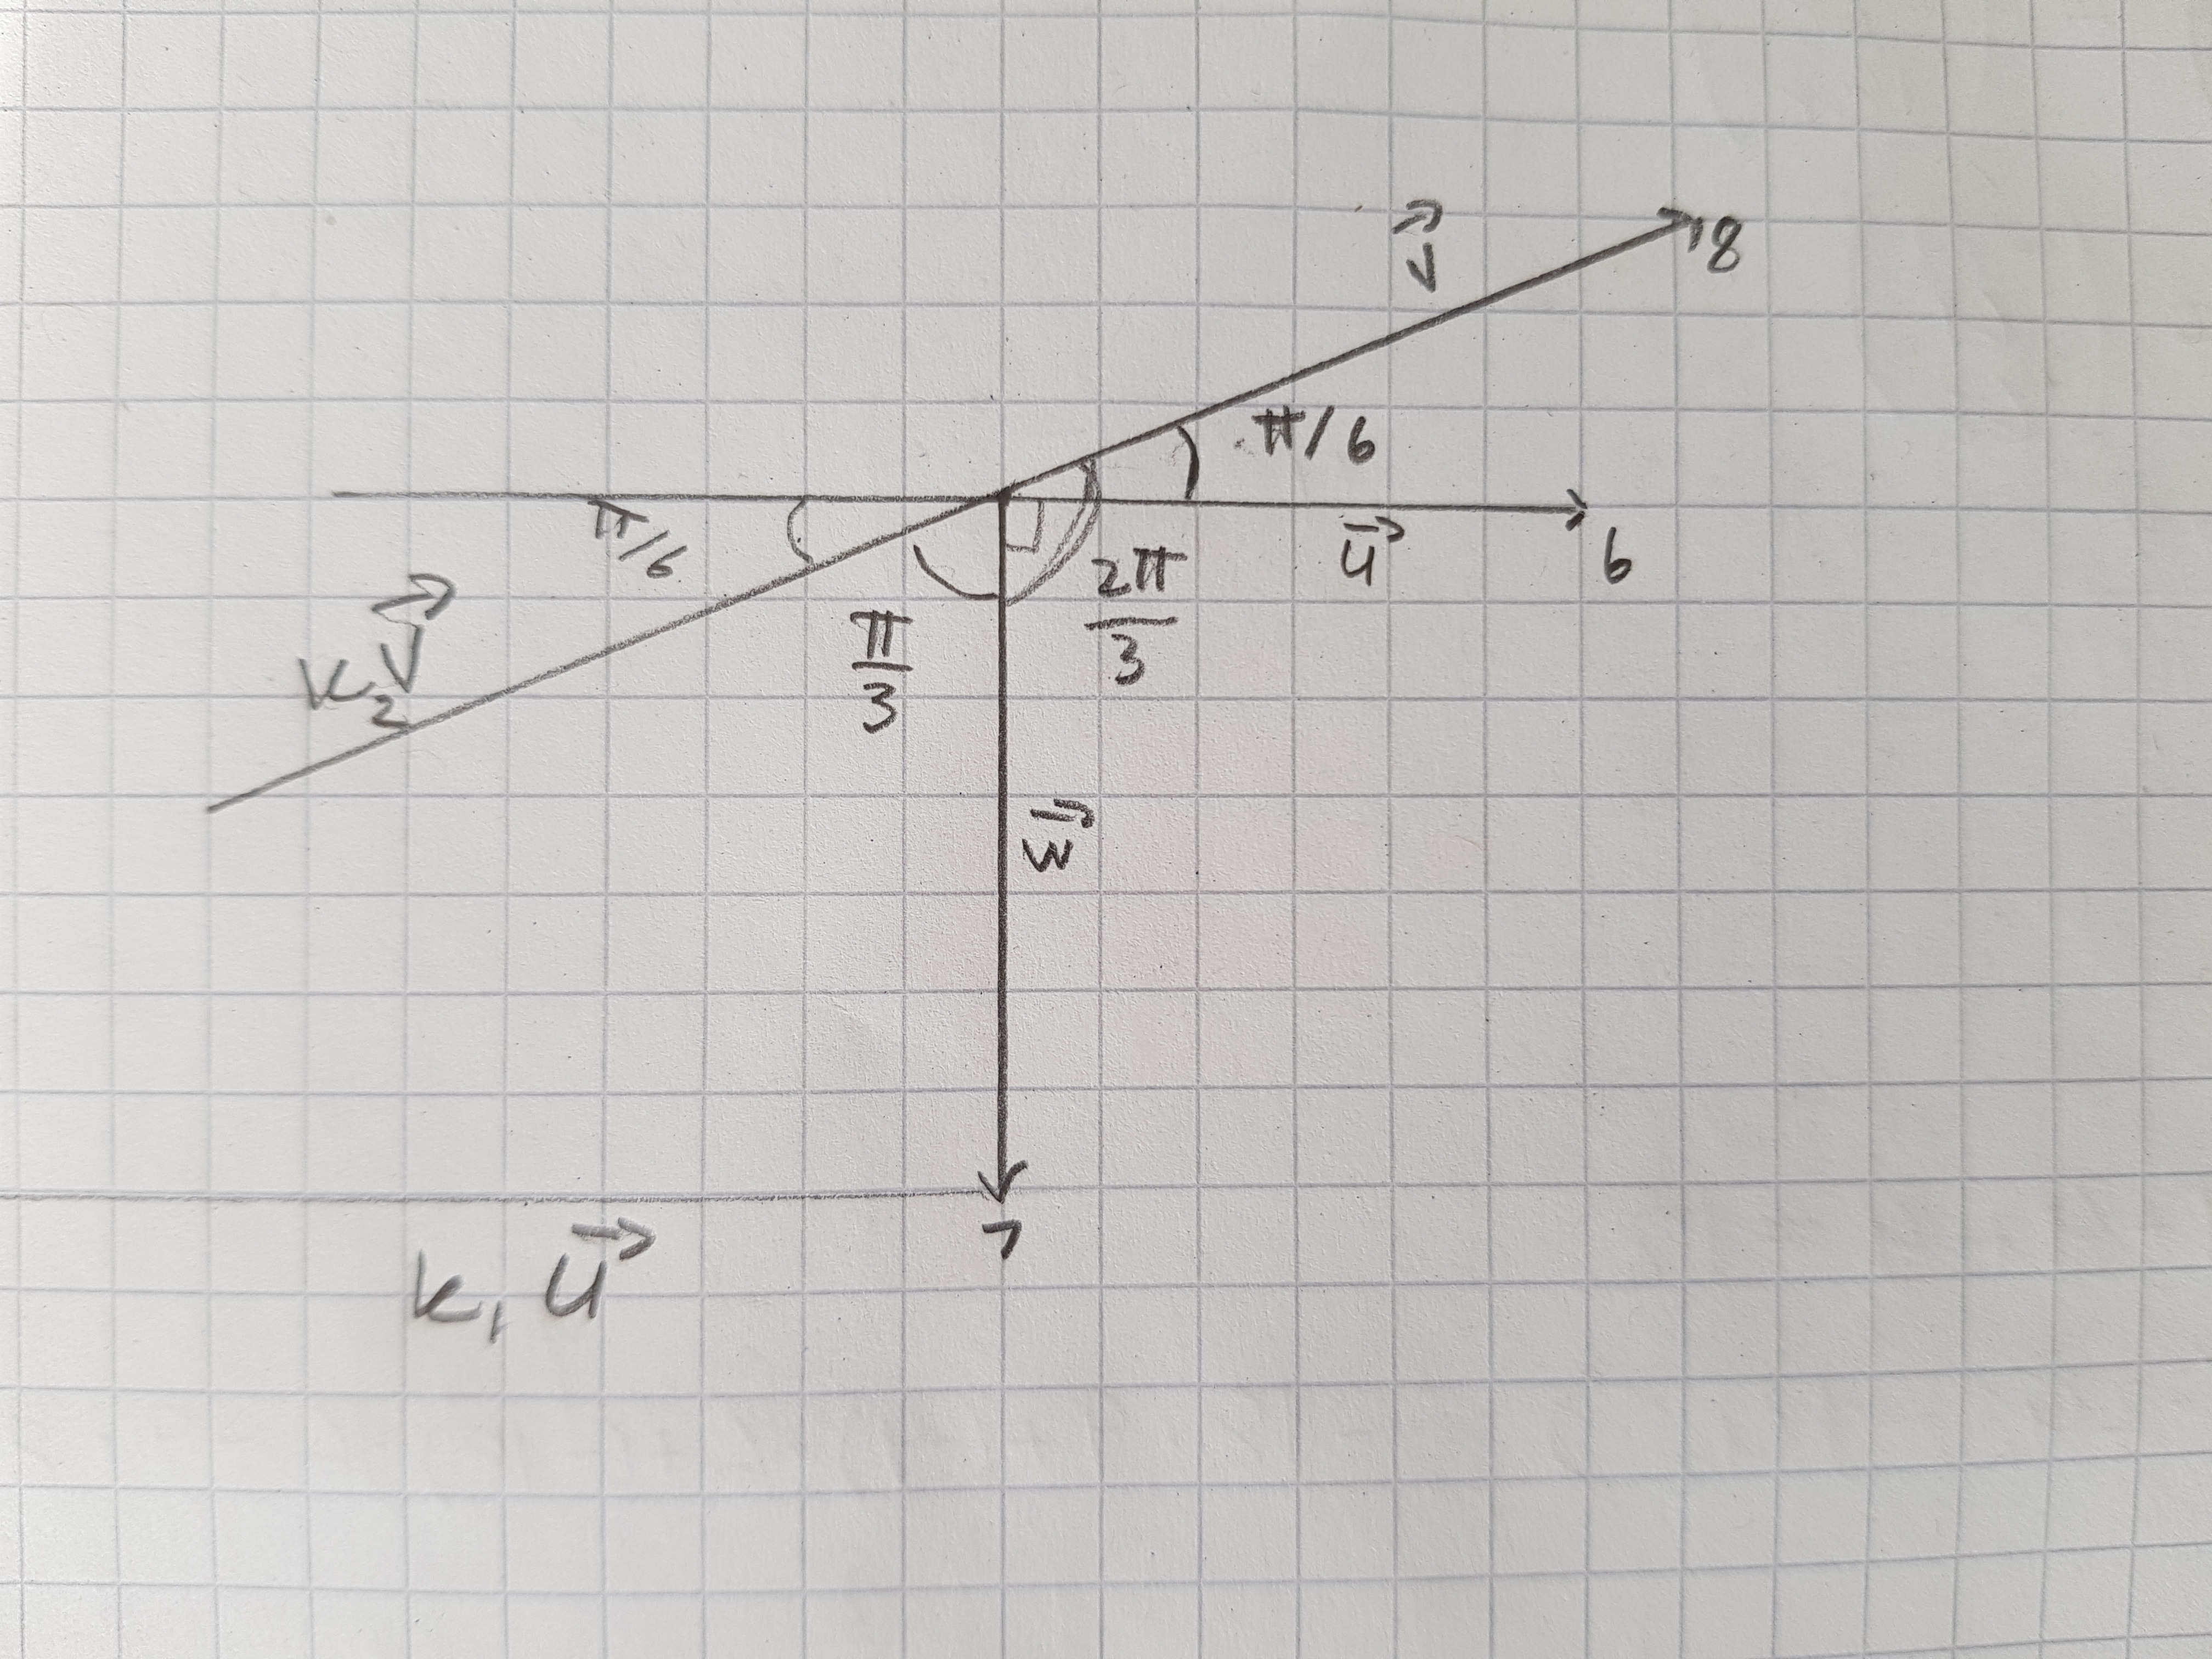
\includegraphics[width=10cm, height=6cm]{image/2.5.8.b.jpg} 
    \caption{2.5.8.b}
\end{figure}


\newpage

\subsection{Area och Volym}
%\textbf{Vektorprodukten räkneregler}
\begin{align*} 
  &\quad  \text{Area parralelogram: } |\vec{u}||\vec{v}|\sin{\theta} = |\vec{u}\times\vec{v}| \\
  &\quad  \text{Volym parralelogram: } |(\vec{u}\times\vec{v})\bullet\vec{w}|
\end{align*}

\begin{figure}[h]
    \vspace{10mm}
    \centering
    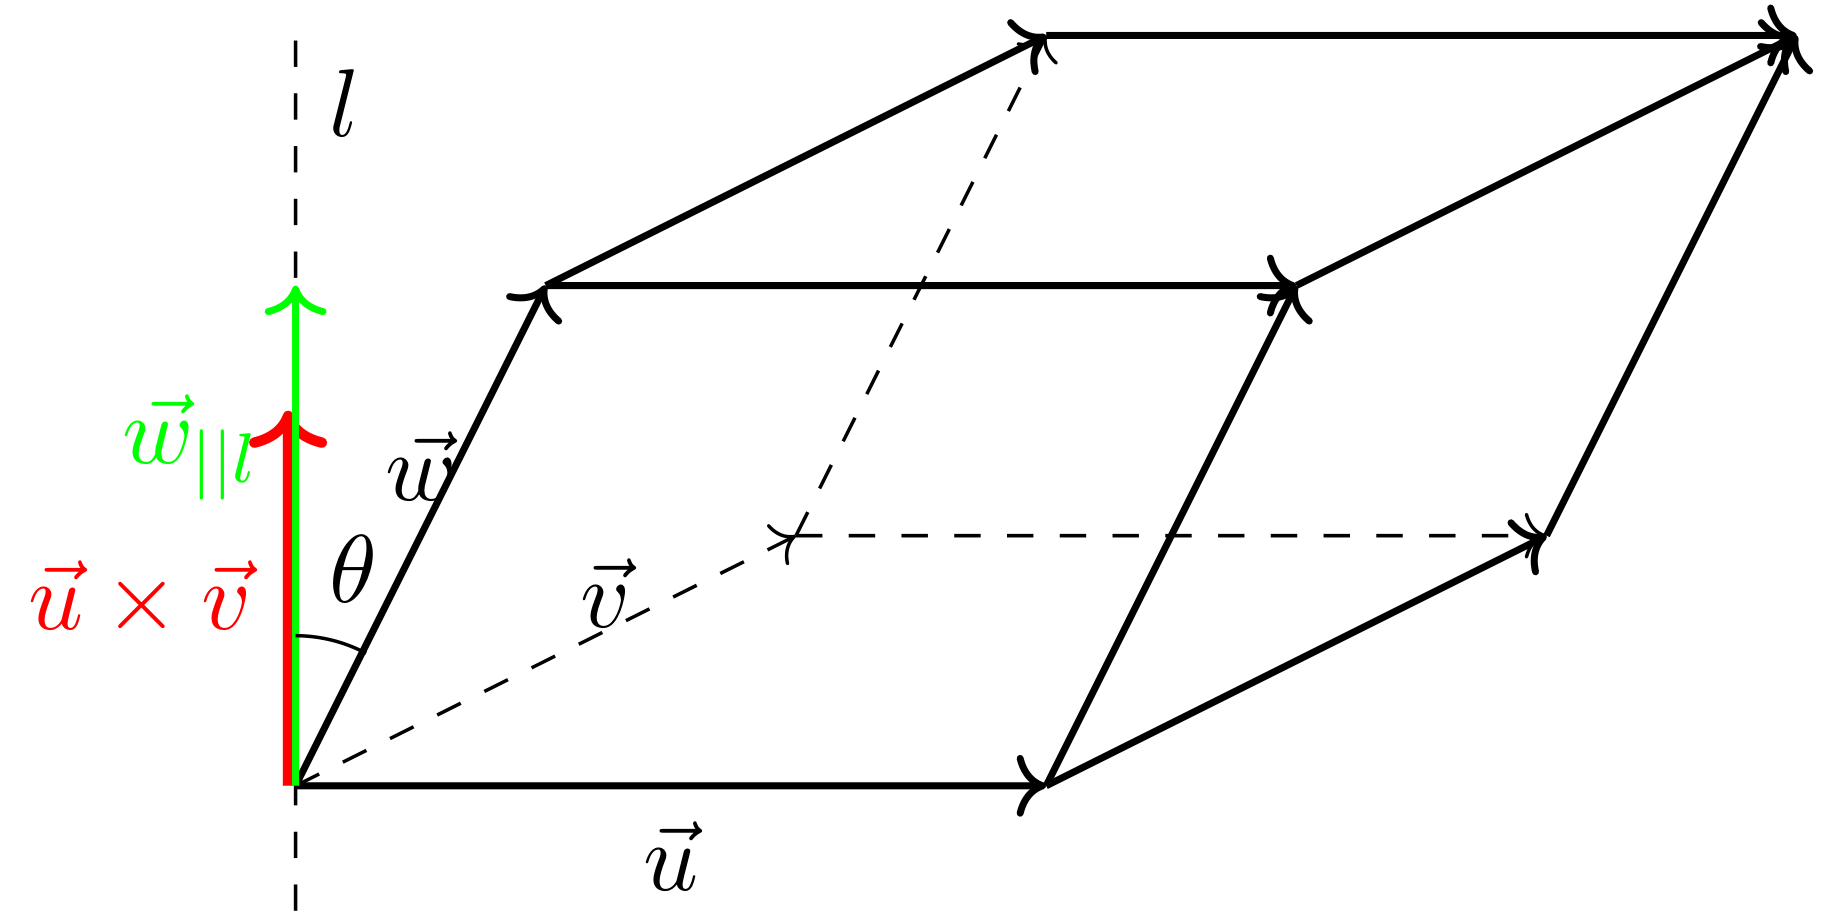
\includegraphics[width=11cm, height=6cm]{image/parallelogram.png} 
    \caption{Ortogonal projektion}
\end{figure}

\textbf{Exempel: Hitta volymen}
\begin{align*} 
  &\quad  \text{Hitta volymen av parallellipipeden med sidorna } \\
  &\quad
  \vec{u} = \begin{pmatrix} 1 \\ 1 \\ 1 \end{pmatrix}
  \vec{v} = \begin{pmatrix} 2 \\ 1 \\ 1 \end{pmatrix}
  \vec{w} = \begin{pmatrix} 1 \\ 1 \\ 2 \end{pmatrix} \\
  &\quad  \text{och avgör om $(\vec{u} \vec{v} \vec{w})$ är ett högersystem,} \\
  &\quad  \text{ett vänstersystem, eller ej en bas.} \\
  &\quad  \\
  &\quad  \text{Lösning: Vi beräknar} \\
  &\quad  \vec{u}\times\vec{v} =
  \begin{pmatrix} 1\cdot{1}-1\cdot{1} \\ 1\cdot{2}-1\cdot{1} \\ 1\cdot{1}-1\cdot{2} \end{pmatrix}
  = \begin{pmatrix} 0 \\ 1 \\ -1 \end{pmatrix} \\
  &\quad  (\vec{u}\times\vec{v})\bullet\vec{w} = 0+1-2=-1 \\
  &\quad  \text{Så det är ett vänstersystem och volymen är 1} \\
\end{align*}


\newpage

\section{Linjer och plan}
\begin{align*} 
  &\quad  \text{Parameterform: }
  \begin{pmatrix} x \\ y \\ z \end{pmatrix} =
  \begin{pmatrix} a_1 \\ a_2 \\ a_3 \end{pmatrix} +
  t\begin{pmatrix} v_1 \\ v_2 \\ v_3 \end{pmatrix}, t \in\mathbb{R} \\
  &\quad  \text{Normalform: } ax+by=c \Rightarrow
  \vec{n} = \begin{pmatrix} a \\ b \end{pmatrix} \\
  &\quad  \text{Plan: }
  \begin{pmatrix} x \\ y \\ z \end{pmatrix} =
  \begin{pmatrix} p_1 \\ p_2 \\ p_3 \end{pmatrix} +
  t\begin{pmatrix} u_1 \\ u_2 \\ u_3 \end{pmatrix} +
  s\begin{pmatrix} v_1 \\ v_2 \\ v_3 \end{pmatrix} \\
\end{align*}


\textbf{Exempel: Skriv i parameterform}
\begin{align*} 
  &\quad  \text{Om vi lösar ekvationen (vars lösningar är en linje): } x+3y=4; \\
  &\quad  y=t \Rightarrow x=4-3t \Rightarrow 
  \begin{pmatrix} x \\ y \end{pmatrix} =
  \begin{pmatrix} 4 \\ 0 \end{pmatrix} +
  t\begin{pmatrix} -3 \\ 1 \end{pmatrix} \\
  &\quad  \text{Hitta parameterform för linje genom givna punkter} \\
  &\quad 
  A= \begin{pmatrix} -21 \\ 20 \end{pmatrix},
  B= \begin{pmatrix} -24 \\ -22 \end{pmatrix} \\
  &\quad  \overline{AB} = \overline{OB}-\overline{0A} =
  \begin{pmatrix} -24-(-21) \\ -22-20 \end{pmatrix} =
  \begin{pmatrix} -3 \\ -42 \end{pmatrix} \Rightarrow \\
  &\quad  L:\underline{e}\begin{pmatrix} x \\ y \end{pmatrix} =
  \underline{e}\begin{pmatrix} -21 \\ 20 \end{pmatrix} +
  t\underline{e}\begin{pmatrix} -3 \\ -42 \end{pmatrix} \\
\end{align*}


\textbf{Exempel: Hitta planets ekvation}
\begin{align*}
  &\quad  \text{Uppgift: Hitta en ekvation för planet som } \\
  &\quad  \text{går genom $(1, 2, 3)$ och är parallell med vektorna } \\
  &\quad
  \vec{u} = \begin{pmatrix} 4 \\ 5 \\ 6 \end{pmatrix}
  \vec{v} = \begin{pmatrix} 7 \\ 8 \\ 9 \end{pmatrix} \\
  &\quad  \\
  &\quad  \text{Lösnig: Vi måste hitta en vektorn $\vec{n}$ som är ortogonal mot planet}  \\
  &\quad  \text{Inte så lätt i 3D som för linje i 2D. Men vi har en formel.} \\
  &\quad
  \vec{n} = \begin{pmatrix} 4 \\ 5 \\ 6 \end{pmatrix} \times
  \begin{pmatrix} 7 \\ 8 \\ 9 \end{pmatrix} =
  \begin{pmatrix} 45-48 \\ 42-36 \\ 32-35 \end{pmatrix} =
  \begin{pmatrix} -3 \\ 6 \\ -3 \end{pmatrix} \\
  &\quad  \text{Det kan vi skriva på normal formen: }
  -3x+6y-3z=c \\
  &\quad  \text{För att hitta $c$ så insätter vi det kända punkten $(1,2,3)$} \\
  &\quad  c = -3\cdot{1}+6\cdot{2}-3\cdot{3} = 0 \\
  &\quad  \text{Vi får formen: } -3x+6y-3z=0 \\
\end{align*}


\textbf{Exempel: Beskriva linje på normalform} 
\begin{align*} %https://www.youtube.com/watch?v=kam3foz8eqA
  &\quad  \text{Uppgift: Hitta normalvektorn för linje } A=(16,4), B=(9,12) \\
  &\quad  \overline{AB} = 
  \begin{pmatrix} 9-16 \\ 12-4 \end{pmatrix} = \begin{pmatrix} -7 \\ 8 \end{pmatrix} \\
  &\quad  L: \overline{OA}+t\overline{AB}=
  \begin{pmatrix} 16 \\ 4 \end{pmatrix} + t\begin{pmatrix} -7 \\ 8 \end{pmatrix} \\
  &\quad  \left\{\begin{array}{r}
  x=16-7t \\
  y=4+8t  
  \end{array}\right. \\
  &\quad  t=\frac{16-x}{7}=\frac{y-3}{8} \Leftrightarrow{} 128 -8x=7y-21 \\
  &\quad  8x+7y=149 \\
\end{align*}
%  &\quad  \text{Uppgift: Hitta normalvektorn för plan} \\

\textbf{Exempel: Skärning mellan plan} %https://www.youtube.com/watch?v=DrD4mBq6_4Q
\begin{align*} %% antat exempel
  &\quad  \left\{\begin{array}{r}
  -3x+y+4z=4 \\
  x-4y-5z=-5 
  \end{array}\right. \\
  &\quad  \\
  &\quad  \left\{\begin{array}{r}
  0-11y-11z=-11 \\
  x-4y-5z=-5 
  \end{array}\right. \\
  &\quad  \left\{\begin{array}{r}
  0+y+z=1 \\
  x-4y-5z=-5 
  \end{array}\right. \\
  &\quad  \left\{\begin{array}{r}
  x+0-z=-1 \\
  0+y+z=1 
  \end{array}\right. \\
  &\quad  \begin{pmatrix} t-1 \\ 1-t \\ t \end{pmatrix} \\
\end{align*}


\textbf{Exempel: Skärning mellan plan och linjen} %https://www.youtube.com/watch?v=Av0wOqkLojU
\begin{align*} %% antat exempel
  &\quad  3x+3y+4z=-7 \\
  &\quad  \left\{\begin{array}{r}
  x = 2-3t \\
  y = 1-3t \\
  z = 3t
  \end{array}\right. \\
  &\quad  3(2- 3t)+3(1 -3t)+4(3t)=-7 \Rightarrow{} -6t=-16  \Rightarrow{} t=\frac{8}{3} \\
  &\quad  \left\{\begin{array}{r}
  x = 2-3t = -6 \\
  y = 1-3t = -7 \\
  z = 3t = 8 
  \end{array}\right. \\
\end{align*}



\newpage

\subsection{ortogonal projektion på plan}
\begin{figure}[h]
    \vspace{10mm}
    \centering
    \includegraphics[width=14cm, height=6cm]{image/ortogonal_projektion_på_plan.png} 
    \caption{Ortogonal projektion på plan}
\end{figure}

\textbf{Exempel: Hitta närmaste punkten i planet} %https://www.youtube.com/watch?v=749xxpKLvzQ
\begin{align*}
  &\quad  \text{Uppgift: hitta närmaste punkten $N$ till punkten } A = (1,-5,2) \\
  &\quad  \text{i planet } P: x+2y-z=1 \text{ Hitta även avståndet mellan $A$ och planet} \\
  &\quad  \\
  &\quad  \text{Lösning: Först väljer vi godtycklig punkt } Q=(1,0,0)
  \text{ i planet, och beräknar} \\
  &\quad  \vec{v}=\overrightarrow{QA} =
  \begin{pmatrix} 1-1 \\ -5 \\ 2 \end{pmatrix} =
  \begin{pmatrix} 0 \\ -5 \\ 2 \end{pmatrix} \\
  &\quad  \text{Normalvektor till planet } x+2y-z=1
  \vec{n} = \begin{pmatrix} 1 \\ 2 \\ -1 \end{pmatrix} \\
  &\quad  \vec{v}_{||\vec{n}} = \frac{0\cdot{1}+(-5)\cdot{2}+2\cdot{(-1)}}{1^2+2^2+{(-1)}^2}\vec{n}
  = -2\vec{n} \\
  &\quad  \text{Så vi får koordinaterna: } \\
  &\quad  \overrightarrow{ON} = \overrightarrow{OA} - \overrightarrow{AN}
  = \overrightarrow{OA}-\vec{v}_{||\vec{n}} =
  \begin{pmatrix} 1 \\ -5 \\ 2 \end{pmatrix} - (-2)\vec{n} =
  \begin{pmatrix} 3 \\ -1 \\ 0 \end{pmatrix} \\
  &\quad  \text{så närmaste punkten är $N = (3,-1,0)$ Avståndet är } |-2\vec{n}| = 2\sqrt{6} \\
\end{align*}

\textbf{Exempel: Hitta närmaste punkten på linje till linje} %F10
\begin{align*}
  &\quad  \text{Hitta den punkt på linjen } \\
  &\quad  
  l: \begin{pmatrix} x \\ y \\ z \end{pmatrix} = \begin{pmatrix} -1 \\ 0 \\ 0 \end{pmatrix} +
  t\begin{pmatrix} 1 \\ 1 \\ 1 \end{pmatrix}, \, t\in\mathbb{R} \\
  &\quad  \text{som är närmast linjen } \\
  &\quad
  k: \begin{pmatrix} x \\ y \\ z \end{pmatrix} = \begin{pmatrix} -1 \\ 0 \\ -1 \end{pmatrix} +
  s\begin{pmatrix} 1 \\ 2 \\ 1 \end{pmatrix}, \, s\in\mathbb{R} \\
  &\quad  A=(-1+t,t,t), \, B=(-1+s,2s,-1+s) \\
  &\quad  \overrightarrow{AB}=
  \begin{pmatrix} (-1+s)-(-1+t) \\ (2s)-(t) \\ (-1+s)-(t) \end{pmatrix} =
  \begin{pmatrix} s-t \\ 2s-t \\ -1+s-t \end{pmatrix} \\
  &\quad  \text{Vektorn ska vara ortogonal mot: }
  \begin{pmatrix} 1 \\ 1 \\ 1 \end{pmatrix} \land
  \begin{pmatrix} 1 \\ 2 \\ 1 \end{pmatrix} \\
  &\quad
  \left\{\begin{array}{r}
  1(s-t) + 1(2s-t) + 1(-1+s-t) = 0  \\
  1(s-t) + 2(2s-t) + 1(-1+s-t) = 0  
  \end{array}\right. =
  \left\{\begin{array}{r}
  -1 + 4s + -3t = 0  \\
  -1 + 6s + -4t = 0 
  \end{array}\right. \\
  &\quad  \Rightarrow{} s=\frac{3t+1}{4} \Rightarrow{} -1 + \frac{3}{2} (3t+1) -4t = 0 \\
  &\quad 
  \left\{\begin{array}{r}
  t=-1  \\
  s=-1/2
  \end{array}\right. \text{(Kontrollera)} -1 -2 +3 = 0, \, -1 -3 +4 = 0 \\
  &\quad  A= (-2,-1,-1), \, B= (-3/2,-1,-3/2)  \Rightarrow\overrightarrow{AB}=
  \begin{pmatrix} 1/2 \\ 0 \\ -1/2 \end{pmatrix} \\
  &\quad  \text{Svar: punkten på linjen $l$ är } A= (-2,-1,-1) \\
\end{align*}


\newpage

\section{Matrisräkning}
\textbf{Begräpp: matriser}
\begin{align*} 
  &\quad  \text{diagonal} \\
  &\quad  \text{huvuddiagonalen} \\
  &\quad  \text{Kummuterar: } AB=BA \\
  &\quad  A={(a_{ij})}_{r\times{k}} \\
  &\quad  \text{Rang: antalet ledande kofisent i trappsteksmatris } \\ 
\end{align*}

\textbf{Räkneregler: matriser}
\begin{align*}
  &\quad  \text{Addition: endast i sama form} \\
  &\quad  \text{Multiplication: } (r\times{k})(k\times{m}) \Rightarrow r\times{x}  \\
  &\quad  (AB)C=A(BC) \\
  &\quad  \lambda(AB) = (\lambda{A})B = A(\lambda{B}) \\
  &\quad  A(B+C) = AB + AC \\
  &\quad  (B+C)A = BA+CA \\
\end{align*}

\begin{figure}[h]
    \vspace{10mm}
    \centering
    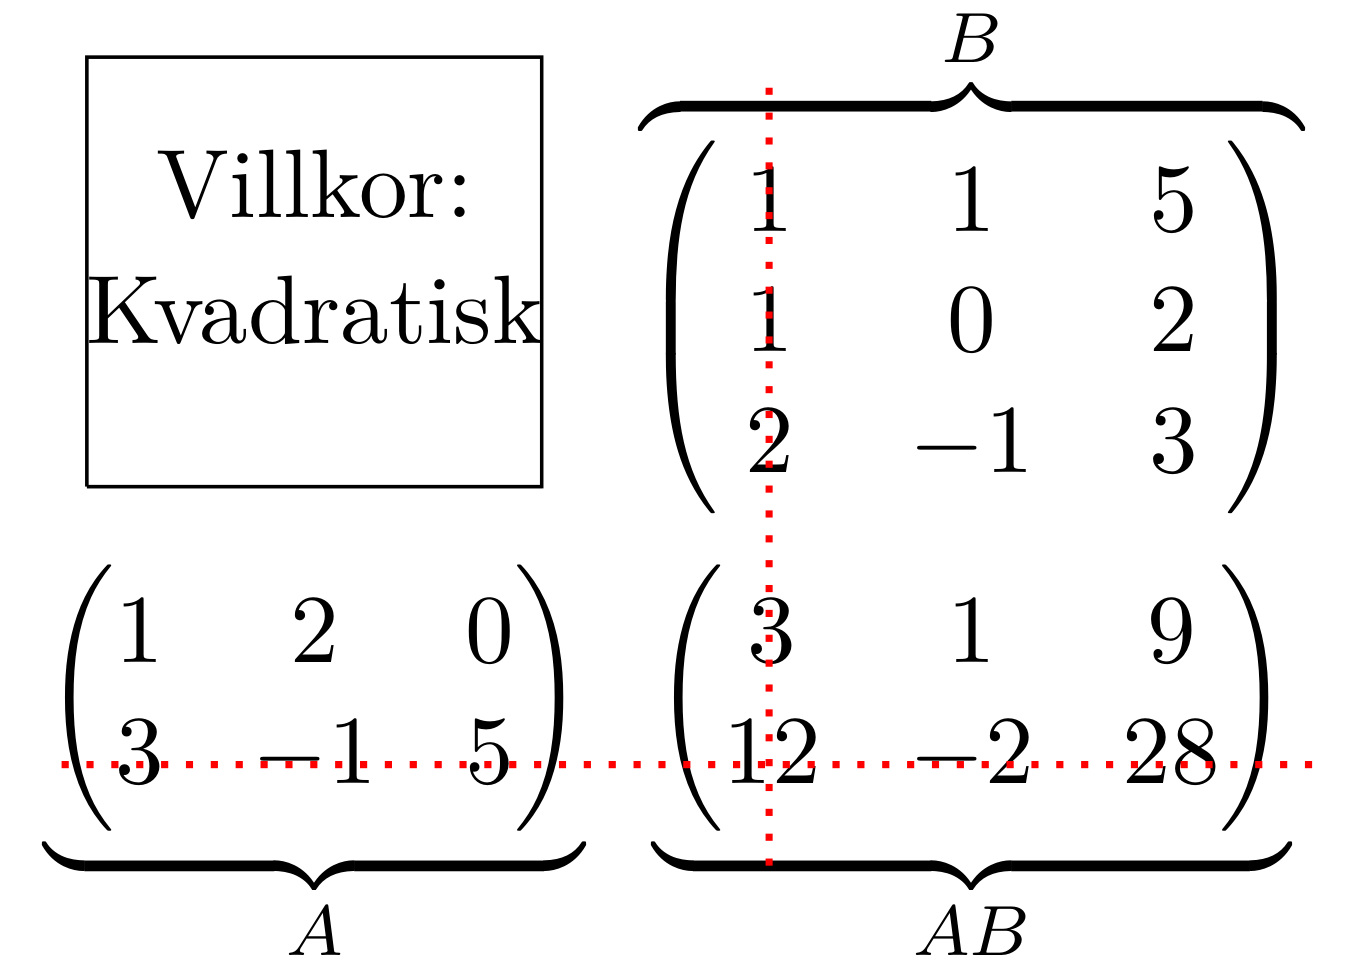
\includegraphics[width=10cm, height=6cm]{image/matris-multiplikation.png} 
    \caption{Ortogonal projektion på plan}
\end{figure}

\textbf{Exempel: Multiplication av matriser}
\begin{align*}
  &\quad
  \left(\begin{array}{ccc}
    2  & 3  & 4 \\
    -1 & 2  & 2 \\
    -5 & -2 & 1 
  \end{array}\right)
  \left(\begin{array}{c}
    a \\
    b \\
    c 
  \end{array}\right) =
  \left(\begin{array}{ccc}
    2a  & 3b  & 4c \\
    -a & 2b  & 2c \\
    -5a & -2b & c 
  \end{array}\right)
\end{align*}

\textbf{Definition: Enhetsmatrisen}
\begin{align*}
  &\quad  \text{Enhetsmatrisn } I_n \\
  &\quad  A^0I_n = I_n \\
  &\quad  A: 2\times{2} AI_2 = A \\
  &\quad  I_3 =
  \left(\begin{array}{ccc}
    1 & 0 & 0 \\
    0 & 1 & 0 \\
    0 & 0 & 1 
  \end{array}\right)
\end{align*}


\subsection{Transpornat}
\textbf{Definition: Transponaten}
\begin{align*}
  &\quad  A^t \text{ betyder inte A upphöjt till t} \\
  &\quad  A={(a_{ij})}_{r\times{k}} \Rightarrow A^t=A={(\alpha_{ij})}_{k\times{r}} \\
  &\quad  A={(\alpha_{ij})}={(a_{ij})}  \\
\end{align*}

\textbf{Exempel: Transponaten}
\begin{align*}
  &\quad  \text{Symetrisk } A=A^t \\
  &\quad
  \left(\begin{array}{cccc}
    1 & 2 & 3 & 4 \\
    5 & 6 & 7 & 8
  \end{array}\right)^t =
  \left(\begin{array}{cc}
    1 & 5 \\
    2 & 6 \\
    3 & 7 \\
    4 & 8
  \end{array}\right)
\end{align*}

\textbf{Räkneregler: Transponaten}
\begin{align*}
  &\quad  {(A+B)}^t = A^t+B^t \\
  &\quad  {(\lambda A)}^t = \lambda A^t \\
  &\quad  {(A^t)}^t = A \\
  &\quad  {(AB)}^t = B^t A^t \\
\end{align*}


\subsection{Matrisinvers}
% X=X_p+X_h
\textbf{Räkneregler: Matrisinvers }
\begin{align*}
  &\quad  AB=BA=I \\
  &\quad  \text{Inversen finns endast om matrisen är kvadratisk} \\
  &\quad  A \text{ är inventerba} \\
  &\quad  AX=B \text{ har entydiga lösningar för alla B} \\
  &\quad  AX=0 \text{ har enbart lösningen} X=0 \\
  &\quad  A \text{ har rang} n \\
  &\quad  A \sim I  \text{ (är radekvivalent med) } I
\end{align*}

\textbf{Exempel: Matrisinvers 3x3}
\begin{align*}
  &\quad
  \left(\begin{array}{ccc}
    1 & 2 & 1 \\
    1 & 1 & 0 \\
    0 & 1 & -1 \\
  \end{array}\right) \sim{}
  \left(\begin{array}{ccc|ccc}
    1 & 2 & 1   & 1 & 0 & 0 \\
    1 & 1 & 0   & 0 & 1 & 0 \\
    0 & 1 & -1  & 0 & 0 & 1 \\
  \end{array}\right) \sim{}
  \left(\begin{array}{ccc|ccc}
    1 & 2  & 1  & 1  & 0 & 0 \\
    0 & -1 & -1 & -1 & 1 & 0 \\
    0 & 1  & -1 & 0  & 0 & 1 \\
  \end{array}\right) \sim{} \\
  &\quad
  \left(\begin{array}{ccc|ccc}
    1 & 0  & -1 & -1  & 2    & 0   \\
    0 & 1  & 1  & 1   & -1   & 0   \\
    0 & 1  & 1  & 1/2 & -1/2 & -1/2 \\
  \end{array}\right) \sim{}
  \left(\begin{array}{ccc|ccc}
    1 & 0  & 0  & -1/2  & 3/2  & -1/2   \\
    0 & 1  & 0  & 1/2   & -1/2 & 1/2 \\
    0 & 0  & 1  & 1/2   & -1/2 & -1/2 \\
  \end{array}\right) \sim{} \\
  &\quad
  A^{-1}=
  \left(\begin{array}{ccc}
    -1/2  & 3/2  & -1/2   \\
    1/2   & -1/2 & 1/2 \\
    1/2   & -1/2 & -1/2 \\
  \end{array}\right) = \frac{1}{2}
  \left(\begin{array}{ccc}
    -1  & 3  & -1  \\
    1   & -1 & 1   \\
    1   & -1 & -1  \\
  \end{array}\right)
\end{align*}

\textbf{Räkneregler: Matrisinvers }
\begin{align*}
  &\quad  A =
  \left(\begin{array}{cc}
    a & b  \\
    c & d  \\
  \end{array}\right) \\
  &\quad  A^{-1} = \frac{1}{ad-bc} 
  \left(\begin{array}{cc}
    d  & -b  \\
    -c & a  \\
  \end{array}\right) \\
\end{align*}

%vissa hur man gör kontrolera på exemplerna

\newpage

\section{Determinanter}
Ekvations system har unika lösningar då koefficient matrisen är inventerbar.
Som är ekvivalent med att determinanten är nollskild.

\textbf{Exempel: determinant många led genväg }
\begin{align*}
  &\quad  
  \left(\begin{array}{ccccc}
    3 & 2 & -3 & 24 & 1005 \\
    0 & 1 & 23 & 14 & 15 \\
    0 & 0 & 3  & 7  & -5 \\
    0 & 0 & 2  & 4  & 3 \\
    0 & 0 & 0  & 0  & 5 \\
  \end{array}\right) \\
  &\quad \text{Vi det finns endast två producter som inte inehåller en nol faktor} \\
  &\quad
  \left(\begin{array}{ccccc}
    (3) & 2 & -3 & 24 & 1005 \\
    0 & (1) & 23 & 14 & 15 \\
    0 & 0 & (3)  & (7)  & -5 \\
    0 & 0 & (2)  & (4)  & 3 \\
    0 & 0 & 0  & 0  & (5) \\
  \end{array}\right) = 3\cdot{1}\cdot{3}\cdot{4}\cdot{5}-3\cdot{1}\cdot{6}\cdot{2}\cdot{5}=0
\end{align*}

\textbf{Exempel: determinant 3x3 }
\begin{align*}
  &\quad  
  \left(\begin{array}{ccc}
    1 & 2 & 3  \\
    4 & 5 & 6  \\
    7 & 8 & 9
  \end{array}\right) = \\
  &\quad  =1\cdot{5}\cdot{9}-1\cdot{6}\cdot{8}-2\cdot{4}\cdot{9}+ \\
  &\quad  +2\cdot{6}\cdot{7}+3\cdot{4}\cdot{8}-3\cdot{5}\cdot{7}= \\
  &\quad  =45-48-72+84+96-105=0 \\
\end{align*}

\textbf{Sats:}
\begin{align*}
  &\quad   \text{Om $B$ är matrisen $A$ där man har bytt om på rad $i$ och $j$ är } detA = -detB \\
  &\quad   (1) \text{ Bytt två rader om i $A$ ändras determinaten sitt teken} \\
  &\quad   (2) \text{ Skalas en rad om med $\lambda$ skalas också determinaten om med } \lambda \\
  &\quad   (3) \text{ Addera en rad gånger något på en annan rad i $A$ ändrar inte
    dennas determinant} \\
  &\quad   (4) \text{ } det(A) = det(A^t) \\
  &\quad   det(AB)=det(A)det(B) \\
\end{align*}


\textbf{Exempel: determinant 3x3 }
\begin{align*}
  &\quad  
  \left(\begin{array}{cccc}
    1 & 2 & 3 & 4  \\
    0 & 3 & 8 & 7  \\
    1 & 3 & 6 & 5  \\
    0 & 0 & 2 & 3  \\
  \end{array}\right) \\
  &\quad
  \left(\begin{array}{cccc}
    1 & 2 & 3 & 4  \\
    0 & 3 & 8 & 7  \\
    0 & 1 & 3 & 1  \\
    0 & 0 & 2 & 3  \\
  \end{array}\right) =
  -\left(\begin{array}{cccc}
    1 & 2 & 3 & 4  \\
    0 & 1 & 3 & 1  \\
    0 & 3 & 8 & 7  \\
    0 & 0 & 2 & 3  \\
  \end{array}\right) =
  -\left(\begin{array}{cccc}
    1 & 2 & 3  & 4  \\
    0 & 1 & 3  & 1  \\
    0 & 0 & -1 & 4  \\
    0 & 0 & 2  & 3  \\
  \end{array}\right) \\
  &\quad
    -\left(\begin{array}{cccc}
    1 & 2 & 3  & 4   \\
    0 & 1 & 3  & 1   \\
    0 & 0 & -1 & 4   \\
    0 & 0 & 0  & 11  \\
  \end{array}\right) = -1\cdot{1}\cdot{(-1)}\cdot{11} = 11 \\
\end{align*}


\textbf{Exempel: okännt x (determinant)}
\begin{align*}
  &\quad  
  \left(\begin{array}{cccc}
    1   & x   & x^2 & x^3  \\
    1   & x^2 & x^3 & x^4  \\
    x   & x^2 & x^4 & x^5  \\
    x^2 & x^3 & x^4 & x^6  \\
  \end{array}\right) \\
  &\quad  \\
  &\quad  x
  \left(\begin{array}{cccc}
    1   & x   & x^2 & x^3  \\
    1   & x^2 & x^3 & x^4  \\
    1   & x   & x^3 & x^4  \\
    x^2 & x^3 & x^4 & x^6  \\
  \end{array}\right) = \text{rad 4 -rad 1} x^3  
  \left(\begin{array}{cccc}
    1   & x   & x^2 & x^3  \\
    1   & x^2 & x^3 & x^4  \\
    1   & x   & x^3 & x^4  \\
    1   & x   & x^2 & x^4  \\
  \end{array}\right) =  x^3
  \left(\begin{array}{cccc}
    1   & x   & x^2 & x^3  \\
    1   & x^2 & x^3 & x^4  \\
    1   & x   & x^3 & x^4  \\
    0   & 0   & 0 & x     \\
  \end{array}\right)^{R4} = \\
  &\quad  \text{rad 3 -rad 1} x^3(x^4-x^3)
  \left(\begin{array}{ccc}
    1   & x   & x^2  \\
    1   & x^2 & x^3  \\
    1   & x   & x^3  \\
  \end{array}\right) = x^6(x-1)^2
  \left(\begin{array}{ccc}
    1   & x   & x^2  \\
    1   & x^2 & x^3  \\
    0   & 0   & x  \\
  \end{array}\right) = \\
  &\quad x^6(x-1)(x^3-x^2)  
  \left(\begin{array}{cc}
    1   & x    \\
    1   & x^2  \\
  \end{array}\right) = x^9(x-1)^3=0
\end{align*}
%https://www.youtube.com/watch?v=KMKd993vG9Q


\subsection{Ko-faktorna}
\begin{align*} %https://www.youtube.com/watch?v=KMKd993vG9Q
  &\quad  det(A) = a_{i1}C_{i1}+a_{i2}C_{i2}+\ldots{}+a_{in}C_{in} \text{ där $a_{ij}$ är teknet o $C_{ij}$ är kofisienten} \\
  &\quad  \tilde{A}^t \text{ är alla kofaktorerna från} A C_{ij} \\
  &\quad  det(a^-1)=det(1/det(a)) \\
  &\quad   \\
  &\quad
  \left(\begin{array}{cccc}
    2 & 1  & 1  & -1  \\
    (1) & (0)  & (2)  & (0)  \\
    1 & -2 & 1  & 2  \\
    3 & 1  & -1 & 5  \\
  \end{array}\right)^{R2} =  (-1)^{2+1}\cdot{1}\cdot{}
  \left(\begin{array}{ccc}
    1  & 1  & -1  \\
    -2 & 1  & 2  \\
    1  & -1 & 5  \\
  \end{array}\right) \\
  &\quad + (-1)^{2+2}\cdot{0}\cdot{} 
  \left(\begin{array}{ccc}
    2 & 1  & -1  \\
    1 & 1  & 2  \\
    3 & -1  & 5  \\
  \end{array}\right) + (-1)^{2+3}\cdot{2}\cdot{}
  \left(\begin{array}{ccc}
    2 & 1  & -1  \\
    1 & -2 & 2  \\
    3 & 1  & 5  \\
  \end{array}\right) + (-1)^{2+4}\cdot{0}\cdot{}
  \left(\begin{array}{ccc}
    2 & 1  & 1  \\
    1 & -2 & 1  \\
    3 & 1  & -1  \\
  \end{array}\right) \\
  &\quad  -1(5+2-2-(-1-2-10))+0-2(-20+6-1-(6+4+5))+0 = -18-2\cdot{(-30)} = 42 \\
\end{align*}

\subsection{Geometri: parallellepiped}
\begin{align*}
  &\quad  \begin{pmatrix} u_1 \\ u_2 \\ u_3 \end{pmatrix} \bullet
  \Bigg( \begin{pmatrix} v_1 \\ v_2 \\ v_3 \end{pmatrix} \times \begin{pmatrix} w_1 \\ w_2 \\ w_3 \end{pmatrix} \Bigg)
\end{align*}


\newpage

\section{Vektorer i $\mathbb{R}^n$}
\begin{align*}
  &\quad  \text{Skallär produkt och ärmed längd är samma regler som innan} \\
  &\quad  \text{Vektor mellan punkter är också samma regler} \\
  &\quad  \text{Vinkeln är samma som innan (ortogonal projection)} \\
  &\quad  \text{Vinkel formel: } \theta=\arccos{\frac{\vec{v}\vec{w}}{|\vec{v}||\vec{w}|}} \\
  &\quad  \text{(Cauchy-Schwarz olikheten) logist! } |\vec{v}\bullet\vec{w}|\leq|\vec{v}||\vec{w}|
  (|3-1|\leq|3||-1|)\\
  &\quad  \\
  &\quad  \text{Linjärt oberoende: inga parametrar vid lösning av }
  c_1\vec{v_1}+c_2\vec{v_2}+\ldots{}+c_n\vec{v_n}=\vec{0} \\
  &\quad  \text{Linjära Höljet (spannet): mängden av alla möjliga linjärakombinationer av vektorerna} \\
  &\quad  \text{Det linjära höljet av vektorerna är hela $\mathbb{R}^n$ omm $Rang{V}=n$} \\
  &\quad  \\
  &\quad  \text{Bas definnerar lika dant i fler dimentioner, för att vara en bas $\mathbb{R}^n$} \\
  &\quad  \text{måste de vara linjärt oberoende och det linjära höljet är hela $\mathbb{R}^n$} \\
\end{align*}


\newpage

\section{Linjära avbildningar $\mathbb{R}^n\to\mathbb{R}^m$}
\subsection{Matristransformationer och linjära funktioner}
\textbf{Termenologi}
\begin{align*}
  &\quad  \text{Standardmatris: En matris som multipliseras med argumentet för att få svaret } \\
  &\quad  \text{Sammansätning: Låt } f:A\to B, g: B\to C \\
  &\quad  (g \circ f)(x)=g(f(x)) \\
  &\quad  \text{Vektor produkt: } F: \mathbb{R}^3\to\mathbb{R}^3 \\
  &\quad  F(\vec{x}) = \vec{a}\times\vec{x} \\
\end{align*}

\textbf{Definition: En funktion $T:\mathbb{R}^k\to\mathbb{R}^n$ kallas linjär om den uppfyller:}
\begin{align*}
  &\quad  \text{För alla } \vec{v},\vec{w}\in\mathbb{R}^k
  \text{ och } \lambda\in\mathbb{R} \text{ gäller} \\
  &\quad  (i) \quad T(\vec{v}+\vec{w})=T(\vec{v})+T(\vec{w}) \\
  &\quad  (ii) \quad T(\lambda\vec{v})=\lambda T(\vec{v}) \\
\end{align*}

\textbf{Formel standard matris}
\begin{align*}
  &\quad  [T]
  \begin{gmatrix}[p]
    | & | & & | \\
    \vec{v_1} & \vec{v_2} & \ldots & \vec{v_k} \\
    | & | & & |
  \end{gmatrix} =
  \begin{gmatrix}[p]
    | & | & & | \\
    T(\vec{v_1}) & T(\vec{v_2}) & \ldots & T(\vec{v_k}) \\
    | & | & & |
  \end{gmatrix}  \\
\end{align*}


\textbf{Exempel: hitta standard matris}
\begin{align*}
  &\quad  \text{Hitta standardmatrisen $[T]$ för den linjära funktionen } T:\mathbb{R}^2\to\mathbb{R}^3
  \text{ som uppfyller att} \\
  &\quad
  T \begin{pmatrix} 0 \\ -4 \end{pmatrix} = \begin{pmatrix} 8 \\ 8 \\ -8 \end{pmatrix} \, \land \,
  T \begin{pmatrix} -1 \\ -1 \end{pmatrix} = \begin{pmatrix} -1 \\ 0 \\ -4 \end{pmatrix} \\
  &\quad  [T]
  \begin{gmatrix}[p]
    0 & -1 \\
    -1 & -1
  \end{gmatrix} =
  \begin{gmatrix}[p]
    8 & -1 \\
    8 &  0 \\
   -8 & -4 
  \end{gmatrix} \\
  &\quad  [T]=
  \begin{gmatrix}[p]
    8 & -1 \\
    8 &  0 \\
   -8 & -4 
  \end{gmatrix} 
  {\begin{gmatrix}[p]
    0 & -1 \\
    -1 & -1
  \end{gmatrix}}^{-1} =
  \begin{gmatrix}[p]
    3 & -2 \\
    2 & -2 \\
    2 &  2
  \end{gmatrix} \\
  &\quad  \\
  &\quad  \text{Kontrol: multiplisera standard matrisen med input och få output} \\
\end{align*}

\textbf{Exempel: hitta standard matris ortogonal projection}
\begin{align*}
  &\quad  \text{Hitta standardmatrisen för } P:\mathbb{R}^3 \to \mathbb{R}^3 \\
  &\quad  \text{där P är den ortogonala projektionen på planet} \pi: 2 x + y + 3 z = 0 \\
  &\quad  \\
  &\quad  T(\vec{n})=T\begin{pmatrix} 2 \\ 1 \\ 3 \end{pmatrix} = \begin{pmatrix} 0 \\ 0 \\ 0 \end{pmatrix} \\
  &\quad  \text{Hittar två godtykliga punkter på planet: }   A=(1,1,-1), \, B=(-1,2,0) \\
  &\quad
  \overrightarrow{OA} = \begin{pmatrix} 1 \\ 1 \\ -1 \end{pmatrix}, \,
  \overrightarrow{OB} = \begin{pmatrix} -1 \\ 2 \\ 0 \end{pmatrix} \\
  &\quad [T]
  \begin{gmatrix}[p]
    3 &  1 & -1  \\
    1 &  1 &  1  \\
    2 & -1 &  0
  \end{gmatrix} =
  \begin{gmatrix}[p]
    0 &  1 & -1  \\
    0 &  1 &  1  \\
    0 & -1 &  0
  \end{gmatrix}  \Rightarrow \\
  &\quad [T] =
  \begin{gmatrix}[p]
    0 &  1 & -1  \\
    0 &  1 &  1  \\
    0 & -1 &  0
  \end{gmatrix}
  {  \begin{gmatrix}[p]
    3 &  1 & -1  \\
    1 &  1 &  1  \\
    2 & -1 &  0
  \end{gmatrix}}^{-1} =
  \begin{gmatrix}[p]
    5/7 & -1/7  & -3/7  \\
   -1/7 & 13/14 & -3/14 \\
   -3/7 & -3/14 &  5/14
  \end{gmatrix} \\
  &\quad  \\
  &\quad  \text{Kontrol: multiplisera standard matrisen med input och få output} \\
\end{align*}

\textbf{Exempel: hitta standard matris spegling}
\begin{align*}
  &\quad  \text{Hitta standardmatrisen för } P:\mathbb{R}^3 \to \mathbb{R}^3 \\
  &\quad  \text{där P är speglingen i planet} \pi: -x + 2y - 2z = 0 \\
  &\quad  \\
  &\quad  T(\vec{n})=T\begin{pmatrix} -1 \\ 2 \\ -2 \end{pmatrix} = \begin{pmatrix} 1 \\ -2 \\ 2 \end{pmatrix} \\
  &\quad  \text{Hittar två godtykliga punkter på planet: }   A=(0,1,1), \, B=(2,1,0) \\
  &\quad
  \overrightarrow{OA} = \begin{pmatrix} 0 \\ 1 \\ 1 \end{pmatrix}, \,
  \overrightarrow{OB} = \begin{pmatrix} 1 \\ 2 \\ 0 \end{pmatrix} \\
  &\quad [T]
  \begin{gmatrix}[p]
   -1 &  0 &  1  \\
    2 &  1 &  2  \\
   -2 &  1 &  0
  \end{gmatrix} =
  \begin{gmatrix}[p]
    1 &  0 &  1  \\
   -2 &  1 &  2  \\
    2 &  1 &  0
  \end{gmatrix}  \Rightarrow \\
  &\quad [T] =
  \begin{gmatrix}[p]
    1 &  0 &  1  \\
   -2 &  1 &  2  \\
    2 &  1 &  0
  \end{gmatrix}
 {\begin{gmatrix}[p]
   -1 &  0 &  1  \\
    2 &  1 &  2  \\
   -2 &  1 &  0
  \end{gmatrix}}^{-1} =
  \begin{gmatrix}[p]
    7/9 &  4/9  & -4/9 \\
    4/9 &  1/9 &   8/9 \\
   -4/9 &  8/9 &   1/9
  \end{gmatrix} \\
  &\quad  \\
  &\quad  \text{Kontrol: multiplisera standard matrisen med input och få output} \\
\end{align*}


\newpage

\subsection{Injektiv/Surjektiv/Bijektiv}
\textbf{Termenologi}
\begin{align*}
  &\quad
  \begin{tabular}{ |c|c|c| } 
    \hline
    [T]           & kolonnvektorerna i [T]                    & funktionen T \\
    \hline
    rang([T])=k   & linjär oberoende                          & injektiv \\ 
    rang([T])=n   & spannet är hela $\mathbb{R}^n$            & surjektiv \\
    n=rang([T])=k & är en bas för $\mathbb{R}^n=\mathbb{R}^k$ & bijektiv \\
    \hline
  \end{tabular} \\
\end{align*}
 \newpage
\chapter{Linear Algebra II}

\newpage

% Gamla tentor
% https://www.studocu.com/sv/document/uppsala-universitet/linjaer-algebra-ii/gamla-tentor/tenta-oktober-2018-fragor/6649302/view
% https://www.studocu.com/sv/document/uppsala-universitet/linjaer-algebra-ii/gamla-tentor/tenta-mars-2016-fragor/3544944/view


\section{Grudläggande teori} % grunden
\subsection{Ekvationssystem och matris räkning}
\begin{align*}
  &\quad \left\{\begin{array}{rr}
  x+2 y+ & z=-1 \\
  2 x+(a+3) y+ & 3 z=-4 \\
  x+(3-a) y+(a-2) z & =a-1
  \end{array}\right. \\
  &\quad \left(\begin{array}{ccc|c}
    1 & 2 & 1 & -1 \\
    2 & a+3 & 3 & -4 \\
    1 & 3-a & a-2 & a-1
  \end{array}\right) \\
  &\quad (-1 \text{ rad1 till rad2}), (-2 \text{ rad1 till rad3}) \\
  &\quad \left(\begin{array}{ccc|c}
    1 & 2 & 1 & -1 \\
    2 & a-1 & 1 & -2 \\
    0 & 1-a & a-3 & a
  \end{array}\right) \\
  &\quad \left(\begin{array}{ccc|c}
    1 & 2 & 1 & -1 \\
    0 & a-1 & 1 & -2 \\
    0 & 0 & a-2 & a-2
  \end{array}\right) \\
  &\quad a \neq 1 \land a \neq 2 \\
  &\quad (\frac{1}{a-2} \text{rad 3}) \\
  &\quad \left(\begin{array}{ccc|c}
    1 & 2 & 1 & -1 \\
    0 & a-1 & 1 & -2 \\
    0 & 0 & 1 & 1
  \end{array}\right) \\
  &\quad (-1 \text{rad 3 till rad 2}), (-1 \text{rad 3 till rad 1}) \\
  &\quad \left(\begin{array}{ccc|c}
    1 & 2 & 0 & -2 \\
    0 & a-1 & 0 & -3 \\
    0 & 0 & 1 & 1
  \end{array}\right) \\
  &\quad (\frac{1}{a-1} \text{rad 2}) \\
  &\quad \left(\begin{array}{ccc|c}
    1 & 2 & 0 & -2 \\
    0 & a-1 & 0 & -3 \\
    0 & 0 & 1 & 1
  \end{array}\right) \\
  &\quad \left(\begin{array}{ccc|c}
    1 & 2 & 0 & -2 \\
    0 & 1 & 0 & \frac{3}{1-a} \\
    0 & 0 & 1 & 1
  \end{array}\right) \\  
  &\quad (-2 \text{rad 2 till rad 3}) \\
  &\quad \left(\begin{array}{ccc|c}
    1 & 0 & 0 & -2 - \frac{6}{1-a} \\
    0 & 1 & 0 & \frac{3}{1-a} \\
    0 & 0 & 1 & 1
  \end{array}\right) \\  
  &\quad \left\{\begin{array}{rr}
  x & = -2 - \frac{6}{1-a} \\
  y & = \frac{3}{1-a} \\
  z & = 1
  \end{array}\right. \\
  &\quad \\
  &\quad \text{\textbf{Kontroll:} stoppar in x,y,z i ekvationerna} \\
  &\quad \left\{\begin{array}{r}
  \left(\frac{2 a-8}{1-a}\right)+\quad 2 \cdot\left(\frac{3}{1-a}\right)+\quad 1=-1 \\
  2 \cdot\left(\frac{2 a-8}{1-a}\right)+(a+3) \cdot\left(\frac{3}{1-a}\right)+\quad 3 \cdot 1=-4 \\
  \left(\frac{2 a-8}{1-a}\right)+(3-a) \cdot\left(\frac{3}{1-a}\right)+(a-2) \cdot 1=a-1
  \end{array}\right.
\end{align*}


\subsection{determinanter}
\begin{align*}
  &\quad  
  \left(\begin{array}{cccc}
    1   & x   & x^2 & x^3  \\
    1   & x^2 & x^3 & x^4  \\
    x   & x^2 & x^4 & x^5  \\
    x^2 & x^3 & x^4 & x^6  \\
  \end{array}\right) \\
  &\quad  \\
  &\quad  x
  \left(\begin{array}{cccc}
    1   & x   & x^2 & x^3  \\
    1   & x^2 & x^3 & x^4  \\
    1   & x   & x^3 & x^4  \\
    x^2 & x^3 & x^4 & x^6  \\
  \end{array}\right) = \text{rad 4 -rad 1} x^3  
  \left(\begin{array}{cccc}
    1   & x   & x^2 & x^3  \\
    1   & x^2 & x^3 & x^4  \\
    1   & x   & x^3 & x^4  \\
    1   & x   & x^2 & x^4  \\
  \end{array}\right) =  x^3
  \left(\begin{array}{cccc}
    1   & x   & x^2 & x^3  \\
    1   & x^2 & x^3 & x^4  \\
    1   & x   & x^3 & x^4  \\
    0   & 0   & 0 & x     \\
  \end{array}\right)^{R4} = \\
  &\quad  \text{rad 3 -rad 1} x^3(x^4-x^3)
  \left(\begin{array}{ccc}
    1   & x   & x^2  \\
    1   & x^2 & x^3  \\
    1   & x   & x^3  \\
  \end{array}\right) = x^6(x-1)^2
  \left(\begin{array}{ccc}
    1   & x   & x^2  \\
    1   & x^2 & x^3  \\
    0   & 0   & x  \\
  \end{array}\right) = \\
  &\quad x^6(x-1)(x^3-x^2)  
  \left(\begin{array}{cc}
    1   & x    \\
    1   & x^2  \\
  \end{array}\right) = x^9(x-1)^3=0
\end{align*}

\subsection{flerdimisionel dvs $R^n$}
räkneregler

\subsection{Funktioner}
polynom functioner vid en viss grad också

\subsection{Linjer}
\begin{align*}
  &\quad  l: \begin{pmatrix} x \\ y \\ z \end{pmatrix} =
  \begin{pmatrix} 3 \\ 2 \\ 5 \end{pmatrix} + t\begin{pmatrix} 1 \\ 2 \\ 2 \end{pmatrix} \\
  &\quad  \text{Då är riktnings vektorn } \begin{pmatrix} 1 \\ 2 \\ 2 \end{pmatrix} \\
  &\quad  \text{Och går genom } \begin{pmatrix} 3 \\ 2 \\ 5 \end{pmatrix} \\
\end{align*}


\newpage

\section{Vektorrum}
\textbf{Definition: vektor rum}
\begin{align*}
  &\quad  \text{En mängd $\mathbb{V}$ kallas för en \underline{reellt vektorrum} om } \\
  &\quad  \text{1. Det finns en operator på  $\mathbb{V}$ som kallas addition och} \\
  &\quad  \text{beräknas med $+$, sådant att om } \vec{u},\vec{v} \in \mathbb{V} \text{ så gäller}  \\
  &\quad  \vec{u}+\vec{v}\in\mathbb{V} \\
  &\quad  \text{2. Det finns en poeration på  $\mathbb{V}$ som kallas skalning eller } \\
  &\quad  \text{multipliseras med reella tal, som beteknas med $\cdot$, sådan } \\
  &\quad  \text{att om } \lambda\in\mathbb{R} \land \vec{v}\in\mathbb{V} \text{ så gäller }
  \lambda\cdot\vec{v}\in\mathbb{V}
\end{align*}
räknereglerna gäller som i la1
%kommutitiva lag, assositiv lag ..

\textbf{Axiomen: vektor rum}
\begin{align*}
  &\quad  \text{1. } \vec{u}+\vec{v} = \vec{v}+\vec{u} \text{ (Kommutativ lag)} \\
  &\quad  \text{2. } \vec{u}(\vec{v}+\vec{w}) = (\vec{u}+\vec{v})+\vec{w} \text{ (Associativ lag)} \\
  &\quad  \text{3. } \text{Det finns ett nollement } \vec{0} \text{ så att }
  \vec{v}+\vec{0}=\vec{v} \\
  &\quad  \text{4. } \text{Till varge } \vec{v}\in\mathbb{V} \text{ finns ett element }
  -\vec{v} \text{ så att} \\
  &\quad  \vec{v}+(-\vec{v}) = 0 \\
  &\quad  \text{5. } 1\cdot\vec{v} = \vec{v} \\
  &\quad  \text{6. } \lambda\cdot(\mu\cdot\vec{v}) = (\lambda\cdot\mu)\cdot\vec{v}
  \text{ (Associativ lag)} \\
  &\quad  \text{7. } (\lambda+\mu)\cdot\vec{v} = \lambda\cdot\vec{v} + \mu\cdot\vec{v}
  \text{ (Distributiv lag)} \\
  &\quad  \text{8. } \lambda\cdot(\vec{u}+\vec{v}) = \lambda\cdot\vec{u} + \lambda\cdot\vec{v}
  \text{ (Distributiv lag)} \\
  &\quad  \forall\lambda,\mu\in\mathbb{R}\land\vec{u},\vec{v},\vec{w}\in\mathbb{V} \\
\end{align*}


\newpage

\section{Underrum och linjära höljet}
Ett underrum är en delmängd $u$ ej $0$ som är sluten under addition och skalning

\textbf{Definition: Underrum}
\begin{align*}
  &\quad  \text{En delmängd $\mathbb{U}$ av ett vektorrum $\mathbb{V}$ kallas för } \\
  &\quad  \text{ett underrum eller delrum av $\mathbb{V}$ om $\mathbb{U}$ är ett vektorrum} \\
  &\quad  \text{med den additionoch den multiplikation med reella tal som definierats i
    $\mathbb{V}$.} \\
\end{align*}

\textbf{Sats: Underrum}
\begin{align*}
  &\quad  \text{En icketom mängd $\mathbb{U}$ av ett vektorrum $\mathbb{V}$ är ett} \\
  &\quad  \text{underrum om och endast om följande gäller} \\
  &\quad  \text{1. Om } \vec{u}\in\mathbb{U} \text{ och } \vec{v}\in\mathbb{U},
  \text{ Så är } \vec{u}+\vec{v} \in\mathbb{U} \\
  &\quad  \text{2. Om } \vec{u}\in\mathbb{U} \text{ och } \lambda\in\mathbb{R},
  \text{ Så är } \lambda\vec{u} \in\mathbb{U} \\
\end{align*}

\textbf{Regler: Underrum}
\begin{align*}
  &\quad  \text{1. Det snabbaste sättet att testa om det gäller är om nollvektorn finns} \\
  &\quad  \text{om den inte gör det så bryter det mot 2-lagen} \\
  &\quad  \text{2. Homogena ekvationer och linjer/plan genonom origo gäller det alltid för} \\
  &\quad  \text{3. Kontunerligt deriverbara, så gäller det att det är ett underrum} \\
\end{align*}

\textbf{Exempel: Underrum (Ex 1)}
\begin{align*}
  &\quad  \text{är } \left\{ \begin{pmatrix} x \\ y \\ z \end{pmatrix} | x+y+z=5 \right\}
  \text{ ett underrum?} \\
  &\quad  \\
  &\quad  \text{Nej, då: } 0+0+0\neq5 \\
\end{align*} %exotisa exempel x=x^2 är ej sant då 2(1 1)^t = (2 2)^t, 2^2\neq2


\textbf{Definition: linjära höljet}
\begin{align*}
  &\quad  \text{En delmängd $\mathbb{U}$ av ett vektorrum $\mathbb{V}$ kallas för } \\
  &\quad  \text{ett underrum eller delrum av $\mathbb{V}$ om $\mathbb{U}$ är ett vektorrum} \\
  &\quad  \text{med den addition och den multiplikation med reella tal som definierats i
    $\mathbb{V}$.} \\
\end{align*}

\textbf{Exempel: Underrum (Ex 4)}
\begin{align*}
  &\quad  \text{Vilka vektrorer i $\mathbb{P}$ tillhör } u=[1, 1+x, 1+x+x^2] \\
  &\quad  \\
  &\quad  \text{Svar: } u=P_2 \text{ (eftersom) } 1\in{u}, x\in{u}, \text{ och } x^2\in{u} \\
  &\quad  \text{Då alla } a\cdot{1} + b\cdot{x} + c\cdot{x^2} \in{u} \\
  &\quad  \text{Inga plynom av grad $>2$ tillhör $u$.} \\
  &\quad  \text{Vi för kombinera det olika elementen i u med addition och multiplication} \\
\end{align*}
% exemepl 5.3.7

\section{Linjärt \(o\)beroende}
\textbf{Ide: linjärt beronde}
\begin{align*}
  &\quad  \text{Om vektorerna kan skrivas om en linjär kombination av det andra vektorerna} \\
  &\quad  \text{så är vektorn linjärt beroende då det inte behöver vektorn} \\
  &\quad  \text{ vi får reda på beoende genom att ställa upp ekv} \\
  &\quad  x_1\vec{v_1}+x_2\vec{v_2} + \ldots{} + x_n\vec{v_n} = \vec{0} \\
  &\quad  \text{Om denna ekvation har icke triviala lösningar (ej noll) då är den beroende} \\
\end{align*}


\textbf{Exempel: om linjärt oberonde}
\begin{align*}
  &\quad  \text{Är mängden }  \Big\{
  \begin{pmatrix} 1 \\ 2  \end{pmatrix}
  \begin{pmatrix} 2 \\ 1  \end{pmatrix} \Big\}
  \text{i $\mathbb{R}^2$ linjärt oberoende}  \\
  &\quad
  x_1\begin{pmatrix} 1 \\ 2  \end{pmatrix} +
  x_2\begin{pmatrix} 2 \\ 1  \end{pmatrix} = \vec{0} 
  \Leftrightarrow
  \left(\begin{array}{cc|c}
    1   & 2  & 0  \\
    2   & 1  & 0  \\
  \end{array}\right) \\
  &\quad  x_1=0, x_2=0 \text{Endast triviala lösningar } \\
\end{align*}

% beviset är att kom av vektor är nollvektorn så flyttar vi över så vn är komb av det andra
% linjär kobinateion kan skrivas på säät med skalär multiplication och addition av elementen/vektorerna


\newpage

\section{Bas}
\textbf{Ide: Bas och Dimention}
\begin{align*}
  &\quad  \text{Bas omm om vektorerna spanner upp hella spannet och det linjärt oberonde} \\
  &\quad  \text{Standard basen } \underline{e} \\
  &\quad  \text{Vi behöver tree vektorer för att utgöra en bas i } \mathbb{R}^3 \text{ är }
  \vec{v_1}, \vec{v_2}, \vec{v_3} \in\mathbb{R}^3 \\
  &\quad  \\
  &\quad  \text{Dimentioner är antallet oberonde vektorer som spänner up ``rummet''} \\
  &\quad  \text{``dimentioner blir då samma som antallet element som en bas av polynom''} \\
  &\quad  \mathbb{P}_3 = a + bx^1 + cx^2 + dx^3 \text{ har 4 dimentioner} \\
  &\quad  \mathbb{R}^3 \text{ har 3 dimentioner} \\
  &\quad  \text{Dimentioner för matriser är } n\times m (2\times{2}-matris = dim 4) \\
  &\quad  \text{En bas med tre vektorer där vektorerna $\mathbb{R}^4$ ger 3 dim} \\
\end{align*}

\textbf{Exempel: Ta fram bas från plan}
\begin{align*}
  &\quad  \text{låt } 2x -y z = 0 \\
  &\quad  \\
  &\quad  \text{Lösning: }  x=y/2 -z/2 \\
  &\quad  \text{Låt } y=s, \, z=t \text{ vi får då lösningen på parameter form} \\
  &\quad  \begin{pmatrix} x \\ y \\ z \end{pmatrix} =
  \begin{pmatrix} s/2 -t/2 \\ s \\ t \end{pmatrix} =
  s/2\begin{pmatrix} 1 \\ 2 \\ 0 \end{pmatrix} +
  t/2\begin{pmatrix} -1 \\ 0 \\ 2 \end{pmatrix} \\
  &\quad  \text{Basen blir då }
  \left( \begin{pmatrix} 1 \\ 2 \\ 0 \end{pmatrix} \begin{pmatrix} -1 \\ 0 \\ 2 \end{pmatrix} \right) \\
\end{align*}


\newpage

\section{Basomvandling}
Vi kan ta inversen av matrisen av vektorerna som utger en bas och få
matrisen som kan multipliseras med vektor för att få omvandlingen.

\textbf{Sats: basbyte}
\begin{align*}
  &\quad  \vec{v}_{\underline{e}} = Tv_{f} \text{ Där T är en matris} \\
  &\quad  T^{\underline{f}}_{\underline{e}} = {(T^{\underline{e}}_{\underline{f}})}^{-1} \\
  &\quad  \vec{v}_{\underline{f}} = T^{\underline{e}}_{\underline{f}} \, \vec{v}_{\underline{e}} \\
\end{align*}

\textbf{Exempel: Från standar till annan bas}
\begin{align*}
  &\quad  \text{Låt } \underline{f}=(f_1 \, f_2) =
  \left( \begin{pmatrix} 2 \\ 1 \\ 1 \end{pmatrix} \begin{pmatrix} 1 \\ 2 \\ 1 \end{pmatrix} \right), \,
  \vec{v} = \begin{pmatrix} -2 \\ 5 \\ 1 \end{pmatrix} \\
  &\quad  \text{Utryck $\vec{v}$ i basen $\underline{f}$} \\
  &\quad  \\
  &\quad  \vec{v}_{\underline{e}} = \begin{pmatrix} -2 \\ 5 \\ 1 \end{pmatrix} =
  x_1 \begin{pmatrix} 2 \\ 1 \\ 1 \end{pmatrix}  + x_2 \begin{pmatrix} 1 \\ 2 \\ 1 \end{pmatrix} \\
  &\quad \left\{\begin{array}{rr}
  2x_1 + x_2 = -2 \\
  x_1 + 2x_2 = 5  \\
  x_1 + x_2 = 1   \\
  \end{array}\right. \Rightarrow{}
  \left(\begin{array}{cc|c}
    2 & 1 & -2   \\
    1 & 2 &  5  \\
    1 & 1 &  1  \\
  \end{array}\right) \sim{}
  \left(\begin{array}{cc|c}
    2 & 1 & -2   \\
    0 & 1 &  4  \\
    0 & 0 &  0  \\
  \end{array}\right)  \\
  &\quad  x_2 = 4, \, x_1 = 1/2(-2 -4) = -3 \Rightarrow{} 
  v_{\underline{f}} = \begin{pmatrix} -3 \\ 4 \end{pmatrix} \\
\end{align*}

\textbf{Exempel: Finn matrisen för bas byte vektorer} % polynom och vektorer
\begin{align*}
  &\quad  \text{Låt } \underline{f} =
  \left( \begin{pmatrix} 1 \\ 1 \end{pmatrix} \begin{pmatrix} 2 \\ 1 \end{pmatrix} \right)
  \text{Bestäm bas omvandling matrisen }   \\
  &\quad  \\
  &\quad  \text{Lös } T^{\underline{e}}_{\underline{f}} = 
  \left(\begin{array}{cc|cc}
    1 & 2 & 1 & 0  \\
    1 & 1 & 0 & 1  \\
  \end{array}\right) \sim
    \left(\begin{array}{cc|cc}
    1 & 0 & -1 &  2  \\
    0 & 1 &  1 & -1  \\
  \end{array}\right) \\
\end{align*}

\textbf{Exempel: Finn matrisen för bas byte polynom}
\begin{align*}
  &\quad  \text{Låt } \underline{e}=(1 \, x) \text{ och } \underline{f}=(1 \, 1-x) \\
  &\quad  \\
  &\quad  \vec{f}_1 = 1 = \vec{e}_1 \Rightarrow \vec{f_1}_e = \begin{pmatrix} 1 \\ 0 \end{pmatrix} \\
  &\quad  \vec{f}_2 = 1-x = \vec{e}_1 - \vec{e}_2 \Rightarrow \vec{f_2}_e = \begin{pmatrix} 1 \\ -1 \end{pmatrix} \\
  &\quad  T^{\underline{f}}_{\underline{e}} =
  \left(\begin{array}{cc}
    1 &  1  \\
    0 & -1  \\
  \end{array}\right) \Rightarrow{} {(T^{\underline{f}}_{\underline{e}})}^{-1} T^{\underline{e}}_{\underline{f}} = \\
  &\quad \left(\begin{array}{cc}
    1 &  1  \\
    0 & -1  \\
  \end{array}\right) \text{} \\
\end{align*}

\textbf{Exempel: Finn matrisen för bas byte mellan olika matriser} 
\begin{align*}
  &\quad  \text{Basbyte mellan } \underline{f} =
  \left( \begin{pmatrix} 1 \\ 1 \end{pmatrix} \begin{pmatrix} 2 \\ 1 \end{pmatrix} \right)
  \text{ och }
  \left( \begin{pmatrix} -1 \\ 1 \end{pmatrix} \begin{pmatrix} 3 \\ 2 \end{pmatrix} \right)
  &\quad  \\
  &\quad  \text{Lös } T^{\underline{g}}_{\underline{f}}: \,
  \left(\begin{array}{cc|cc}
    1 & 2 & -1 & 3  \\
    1 & 1 &  1 & 2  \\
  \end{array}\right) \sim{} \\
  &\quad
  \left(\begin{array}{cc|cc}
    1 & 0 &   3 & 1  \\
    0 & 1 &  -2 & 1  \\
  \end{array}\right) \Rightarrow{}
  \left(\begin{array}{cc}
    3 & 1  \\
   -2 & 1  \\
  \end{array}\right)  \\
\end{align*}


\textbf{Definition: Nollrum, Kolonrum, radrum.} 
\begin{align*}
  &\quad  \text{låt A vara en $m\times n-matris$} \\
  &\quad  \text{1. dim(A:s kolonrum) = dim(A:s radrum) = rang A} \\
  &\quad  \text{2. dim(A:s kolonrum) + dim(A:s nollrum) = n} \\
\end{align*}

\textbf{Exempel: Finn Nollrum, Kolonrum, radrum.} 
\begin{align*}
  &\quad  \text{Hitta en bas för kolonrummet, radrummet och nollrumet} \\
  &\quad  \text{till följande matris. Bestäm även rummens dimensioner} \\
  &\quad  A = 
  \left(\begin{array}{cccc}
    1 & 2 &  3 & 3  \\
    1 & 3 &  4 & 5  \\
   -1 & 0 & -1 & 1  \\
  \end{array}\right)  \\
  &\quad  \\
  &\quad  \text{Låt kolonernana vara vektorer, då får vi följande gäller }  \\
  &\quad  x_1v_1 + x_2v_2 + x_4v_3 + x_4v_4 = 0 \Leftrightarrow{} (v_1 \, v_2 \, v_3 \, v_4)
  \begin{pmatrix} x_1 \\ x_2 \\ x_3 \\ x_4 \end{pmatrix} = 0 \Leftrightarrow{} Ax=0 \\
  &\quad  \text{Gausselimination ger oss } A \sim{}
  \left(\begin{array}{cccc}
    1 & 0 & 1 & -1  \\
    0 & 1 & 1 &  2  \\
    0 & 0 & 0 &  0  \\
  \end{array}\right)  \\
  &\quad
  \begin{pmatrix} x_1 \\ x_2 \\ x_3 \\ x_4 \end{pmatrix} =
  \begin{pmatrix} -s+t \\ -s-2t \\ s \\ t \end{pmatrix} =
  s\begin{pmatrix} -1 \\ -1 \\ 1 \\ 0 \end{pmatrix} +
  t\begin{pmatrix} 1 \\ -2 \\ 0 \\ 1 \end{pmatrix} \\
  &\quad  \text{Basen för nollrumet blir då }
  \left( \begin{pmatrix} -1 \\ -1 \\ 1 \\ 0 \end{pmatrix} \, \begin{pmatrix} 1 \\ -2 \\ 0 \\ 1 \end{pmatrix} \right)  \\
  &\quad  \text{Basen för kolonrumet blir då det vektorer i A som har Pivot element dvs } v_1, v_2 \\
  &\quad
  \left( \begin{pmatrix} 1 \\ 1 \\ -1 \end{pmatrix} \begin{pmatrix} 2 \\ 3 \\ 0 \end{pmatrix} \right) \\
  &\quad  \text{Basen för radrumet blir }
  \left( \begin{pmatrix} 1 \\ 0 \\ 1 \\ -1 \end{pmatrix} \begin{pmatrix} 0 \\ 1 \\ 1 \\ 2 \end{pmatrix} \right) \\
\end{align*}


\section{Linjär avbildning}
\textbf{Definition: Linjär avbilding}
\begin{align*}
  &\quad  \text{låt $\mathbb{V}$ och $\mathbb{W}$ vara vektorrum. En funktion } F:\mathbb{V}\to\mathbb{W} \\
  &\quad  \text{kallas för linjär avbildning omm} \\
  &\quad  \text{1. } F(\vec{v}+\vec{w}) = F(\vec{v}) + F(\vec{w}) \\
  &\quad  \text{2. } F(\lambda\cdot\vec{v}) = \lambda\cdot F(\vec{v}) \\
\end{align*}

\textbf{Exempel: Derivatan av polynom}
\begin{align*}
  &\quad  \text{Är följande en linjär avbildning } \\
  &\quad  F:C^1(a,b)\to{C}(a,b) \text{ definerad genom } F(f)=\frac{df}{dx}  \\
  &\quad  \\
  &\quad  \big( \frac{d}{dx}(af(x) + bg(x)) \big) = a\frac{df}{dx} + b\frac{dg}{dx} \\
  &\quad  ( \frac{d}{dx}(\lambda af(x)) ) = \lambda  ( \frac{d}{dx}(af(x)) ) \\
  &\quad  \text{Svar: ja $F$ är en linjär avbilding} \\
\end{align*}


\section{Matrisen av en linjär avbilding}
\begin{figure}[h]
    \vspace{10mm}
    \centering
    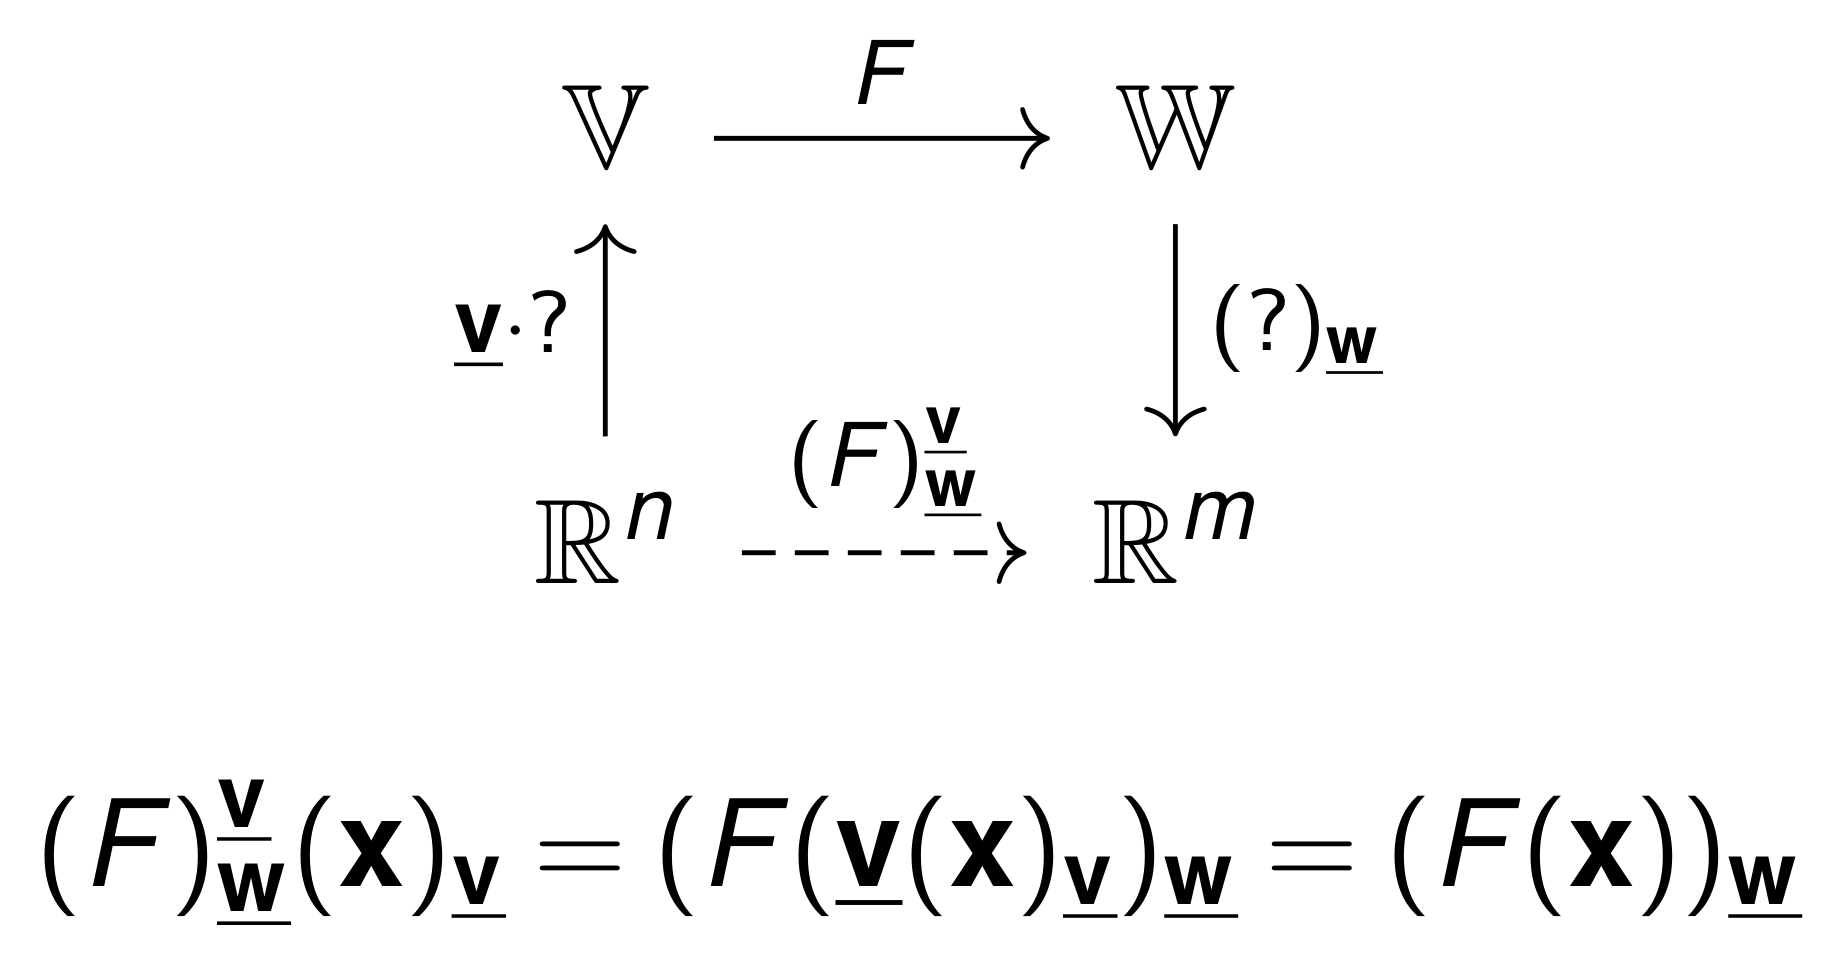
\includegraphics[width=10cm, height=5cm]{image/matris_lin_avb.png} 
    \caption{Matris av en linjär avbildning. From \cite{}}
\end{figure}

\textbf{Exempel: Rotations matrisen}
\begin{align*}
  &\quad
  \left(\begin{array}{cc}
    \cos(\alpha) & -\sin(\alpha)   \\
    \sin(\alpha) &  \cos(\alpha)   \\
  \end{array}\right)  \\
  &\quad
  \left(\begin{array}{ccc}
    1 & 0            & 0               \\
    0 & \cos(\alpha) & -\sin(\alpha)   \\
    0 & \sin(\alpha) &  \cos(\alpha)   \\
  \end{array}\right)  \\
\end{align*}


%\textbf{Exempel: Derivatan av polynom}
%\begin{align*}
%  &\quad  \text{Bestäm matrisen för } \frac{d}{dx}\circ{G}:\mathbb{P}_2\to\mathbb{P}_2
%  \text{och } G\circ\frac{d}{dx}:\mathbb{P}_3\to\mathbb{P}_3 \\
%  &\quad \text{ där } \frac{d}{dx} \\
%  &\quad  G:\mathbb{P}_2\to\mathbb{P}_3 \text{ ges av } F(p(x))=(x+1)p(x) \\
%  &\quad  \frac{d}{dx}\circ{G}(a_0+a_1x+a_2x^2) = \frac{d}{dx}(x+1)(a_0+a_1x+a_2x^2) = \\
%  &\quad  \frac{d}{dx}(a_0 + (a_0+a_1)x + (a_1+a_2)x^2 + a_2x^3) =
%  a_0+a_1 + 2(a_1+a_2)x + 3a_2x^2 \\
%  &\quad  \text{Matrisn ska sltså sicka }
%  \begin{pmatrix} a_0 \\ a_1 \\ a_2 \end{pmatrix} \text{ på }
%  \begin{pmatrix} a_0+a_1 \\ 2a_1+2a_2 \\ 3a_2 \end{pmatrix} \text{ så }
%  {\big( \frac{d}{dx}\circ{G} \big)}^{w}_{w} =
%  \left(\begin{array}{ccc}
%    1 & 1 & 0  \\
%    0 & 2 & 2  \\
%    0 & 0 & 3  \\
%  \end{array}\right)  \\
%  &\quad
%  \left(\begin{array}{cccc}
%    0 & 1 & 0 & 0 \\
%    0 & 0 & 2 & 0 \\
%    0 & 0 & 0 & 3 \\
%  \end{array}\right) 
%  \left(\begin{array}{ccc}
%    1 & 0 & 0  \\
%    1 & 1 & 0  \\
%    0 & 1 & 1  \\
%    0 & 0 & 1  \\
%  \end{array}\right) =
%  \left(\begin{array}{ccc}
%    1 & 1 & 0  \\
%    0 & 2 & 2  \\
%    0 & 0 & 3  \\
%  \end{array}\right) 
%\end{align*}

\textbf{Exempel: Hitta matrisen}
\begin{align*}
  &\quad  \text{Linjär avbildning} F:\mathbb{P}_3\to\mathbb{P}_3, \, F= p+ p'+ p''+ p'''
  \text{Ange $F$:s matris i standarbasen.} \\
  &\quad  \\
  &\quad  \text{Avbildar varge ellement i standardbasen } (1 \, x \, x^2 \, x^3) \\
  &\quad  F(1) = 1 + 1' + 1'' + 1''' = 1 \\
  &\quad  F(x) = x + x' + x'' + x''' = x+1 \\
  &\quad  F(x^2) = {x^2} + {x^2}' + {x^2}'' + {x^2}''' = x^2 + 2x + 2\cdot1 \\
  &\quad  F(x^3) = {x^3} + {x^3}' + {x^3}'' + {x^3}''' = x^3 + 3x^2 + 6x + 6\cdot1 \\
  &\quad
  \left(\begin{array}{cccc}
    1 & 1 & 2 & 6 \\
    0 & 1 & 2 & 6 \\
    0 & 0 & 1 & 3 \\
    0 & 0 & 0 & 1 \\
  \end{array}\right)   
\end{align*}


\newpage

\section{Basbyte av linjära avbildningar}
\textbf{Definition: Basbyte av linjära avblidningar}
\begin{align*}
  &\quad  \text{låt $F: \mathbb{V}\to\mathbb{W}$ vara linjär. Låt $\underline{e}$ och
    $\underline{v}$ vara baser i $\mathbb{V}$ och låt $\underline{f}$} \\
  &\quad  \text{och $\underline{w}$ vara baser av $\mathbb{W}$. Då gäller}  \\
  &\quad   {(F)}^{\underline{e}}_{\underline{f}} =
  T^{\underline{w}}_{\underline{f}}{(F)}^{\underline{v}}_{\underline{w}}T^{\underline{e}}_{\underline{v}} \\
  &\quad   \text{Där vektorn kommer från höger (viktigt vid vilken
    ording transfomations matriserna står)} \\
  &\quad   \\
  &\quad  \text{Ide: Vi omvandlar från en bas (ex standard bas) till en bas som
    är mer anpasat för uträkningen} \\
  &\quad  \text{Sedan omvandlar vi igen för att få svaret i den bas vi vill ha
    den i (ex standard bas)} \\
\end{align*}

\textbf{Exempel: Basbyte av linjär avbildning vektor}
\begin{align*} % q9 fråga 1
  &\quad  \text{} \\
\end{align*}

\textbf{Exempel: Basbyte av linjär avbildning polynom}
\begin{align*}
  &\quad  \text{Vad är matrisen av derivatan } \mathbb{P}_3\to\mathbb{P}_2
  \text{ med avseende på } \\
  &\quad  \text{basen } \underline{u} = (x^3 \, x^2 \, x \, 1) av \mathbb{P}_3 \text{ och }
  \underline{v} = (x^2 \, x \, 1)  \text{ av $\mathbb{P}_2$?}\\
  &\quad  \\
  &\quad  {(H)}^{\underline{e}}_{\underline{f}} =
  \left(\begin{array}{cccc}
    0 & 1 & 0 & 0 \\
    0 & 0 & 2 & 0 \\
    0 & 0 & 0 & 3 \\
  \end{array}\right)  \\
  &\quad  \\
  &\quad  T^{\underline{f}}_{\underline{v}}: \\
  &\quad  \vec{f}_1 = 1   = 0\vec{v}_1 + 0\vec{v}_2 + 1\vec{v}_3 \\
  &\quad  \vec{f}_2 = x   = 0\vec{v}_1 + 1\vec{v}_2 + 0\vec{v}_3 \\
  &\quad  \vec{f}_3 = x^2 = 1\vec{v}_1 + 0\vec{v}_2 + 0\vec{v}_3 \\
  &\quad  \\
  &\quad  T^{\underline{u}}_{\underline{e}}: \\
  &\quad  \vec{u}_1 = x^3 = 0\vec{e}_1 + 0\vec{e}_2 + 0\vec{e}_3 + 1\vec{e}_4 \\
  &\quad  \vec{u}_2 = x^2 = 0\vec{e}_1 + 0\vec{e}_2 + 1\vec{e}_3 + 0\vec{e}_4 \\
  &\quad  \vec{u}_3 = x   = 0\vec{e}_1 + 1\vec{e}_2 + 0\vec{e}_3 + 0\vec{e}_4 \\
  &\quad  \vec{u}_4 = 1   = 1\vec{e}_1 + 0\vec{e}_2 + 0\vec{e}_3 + 0\vec{e}_4 \\
  &\quad  \\
  &\quad  {(H)}^{\underline{u}}_{\underline{v}} =
  T^{\underline{f}}_{\underline{v}} {(H)}^{\underline{e}}_{\underline{f}} T^{\underline{u}}_{\underline{e}} =
  \left(\begin{array}{ccc}
    0 & 0 & 1  \\
    0 & 1 & 0  \\
    1 & 0 & 0  \\
  \end{array}\right) 
  \left(\begin{array}{cccc}
    0 & 1 & 0 & 0 \\
    0 & 0 & 2 & 0 \\
    0 & 0 & 0 & 3 \\
  \end{array}\right) 
  \left(\begin{array}{cccc}
    0 & 0 & 0 & 1 \\
    0 & 0 & 1 & 0 \\
    0 & 1 & 0 & 0 \\
    1 & 0 & 0 & 0 \\
  \end{array}\right)  
\end{align*}



% normalisera

% avmilding matrisen är f^v_w om f:v \to w
% det är avbildingns matrisen om är i mitten av bassbyte formeln?

\section{Kärna och bild av en linjär avbildning}

\textbf{Definition: Kärna och bild}
\begin{align*}
  &\quad  \text{Låt $F:\mathbb{V}\to\mathbb{W}$ vara en linjär avbilding} \\
  &\quad  \\
  &\quad  \text{\textbf{Kärnan} eller \textbf{nollrummet} av den linjära avbildingen F} \\
  &\quad  \ker(F) = N(F) = \{\vec{v}\in\mathbb{V} | F(\vec{v} = \vec{0})\} \\
  &\quad  \\
  &\quad  \text{\textbf{Bilden} eller \text{värderummet} av den linjära avbildingen F} \\
  &\quad  \Ima(F) = V(F) = \{\vec{w}\in\mathbb{W} | \exists\vec{v}:F(\vec{v})=\vec{w}\} \\
\end{align*}

\textbf{Definition: Isomorfism, injektiv, surjektiv }
\begin{align*}
  &\quad  F:X\to{y} \text{ kallas} \\
  &\quad  \text{\textbf{injektiv} om } F(x) = F(x') \Rightarrow x = x' \\
  &\quad  \text{\textbf{surjektiv} om } \forall{y}\in Y\exists{x}\in{X}:f(x)=y \\
  &\quad  \text{\textbf{bijektiv} om det är både injektiv och surjektiv} 
\end{align*}

\textbf{Sats:}
\begin{align*}
  &\quad  \text{Låt $F:\mathbb{V}\to\mathbb{W}$ vara linjär} \\
  &\quad  F \text{ är injektiv omm } \ker{F} = \{\vec{0}\} \\
  &\quad  F \text{ är surjektiv omm } \Ima{F} = \mathbb{W} \text{ omm }
  \Rang ({(F)}^{\underline{u}}_{\underline{w}}) = \dim{\mathbb{W}} \\
\end{align*}


\textbf{Sats: Dimensionssatsen}
\begin{align*}
  &\quad  \text{För varje linjär avbilding $F:\mathbb{V}\to\mathbb{W}$ gäller} \\
  &\quad  \dim{\mathbb{V}} = \dim{\ker(F)} + \dim{\Ima(F)}  \\
\end{align*}

\textbf{Sats: Isomorfism}
\begin{align*}
  &\quad  \text{Låt $F:\mathbb{V}\to\mathbb{W}$ vara en linjär avbilding. De följande är ekvivalenta} \\
  &\quad  F \text{ är en isomorf} \\
  &\quad  \dim{\mathbb{V}} = \dim{\mathbb{W}} \text{ och $F$ är injektiva} \\
  &\quad  \dim{\mathbb{V}} = \dim{\mathbb{W}} \text{ och $F$ är surjektiva} \\
  &\quad  \det({(F)}^{\underline{v}}_{\underline{w}}) \neq 0 \\
  &\quad  {(F)}^{\underline{v}}_{\underline{w}} \text{ är en kvadratisk matris av rang }
  \dim{\mathbb{V}} = \dim{\mathbb{W}} \\
\end{align*}


% körna är att det finns en vektor som ablidast till noll vektorn
% dim ker(f) = antal fria variabler
% dim im(f) = antal priof elementen


\newpage

\section{Egenvärden och egenvektorer}
% definition
\textbf{Definition: Egenvärde och egenvektor}
\begin{align*}
  &\quad  \text{Låt $F:\mathbb{V}\to\mathbb{W}$ vara en linjär avbilding. En vektor} \vec{v}\neq\vec{0} \\
  &\quad  \text{kallas en \textbf{egenvektor} till $F$ om det finns $\lambda\in\mathbb{R}$ så att }
  F(\vec{v}) = \lambda\vec{v} \\
  &\quad  \text{I detta fall kallas $\lambda$ en \textbf{egenvärde} till $F$} \\
  &\quad  \mathbb{V}_{F,\lambda} = \{ \vec{v}\in\mathbb{V} | F(\vec{v}) = \lambda\vec{v} \}
  \text{kallas \textbf{egenrummet} av $F$ till egenvärdet $\lambda$} \\
\end{align*}

% seculärpolynomet
\textbf{Definition: Sekularpolynomet}
\begin{align*}
  &\quad  \text{För en matris $A$ kallas polynomet } \chi_A(\lambda) = \det(A-\lambda I_n) \\
  &\quad  \text{\textbf{sekularpolynomet} till $A$ } \\
  &\quad  \text{Om } A= {(F)}^{\underline{e}}_{\underline{e}}, \text{ så kallas $\chi_A$ också
  sekularpolunomet till $F$} \\
\end{align*}

% ett huvud exempel står i notes
\textbf{Exempel:}
\begin{align*}
  &\quad  F:\mathbb{R}^3\to\mathbb{R}^3 \text{ matrisen i standardbasen är }
  \left(\begin{array}{ccc}
    1 & 2 & 2  \\
    0 & 2 & 1  \\
   -1 & 2 & 2  \\
  \end{array}\right) \\
  &\quad  \\
  &\quad  \text{1. Hittar egenvärderna} \\
  &\quad  F (\vec{x}) = \lambda\vec{x} \Leftrightarrow{} A\vec{x}=\lambda\vec{x} \\
  &\quad  A\vec{x}-\lambda\vec{x} = \vec{0} \Leftrightarrow{} (A-\lambda{I})\vec{x} = 0 \\
  &\quad  \text{Där $\lambda$ är egenvärdet, och $\vec{x}$ är egenvektorn} \\
  &\quad  A-\lambda{I} =
  \left(\begin{array}{ccc}
    1-\lambda & 2         & 2          \\
    0         & 2-\lambda & 1          \\
   -1         & 2         & 2-\lambda  \\
  \end{array}\right) \\
  &\quad  \det(A-\lambda{I}) = 4 -2\lambda{} -(2 -\lambda)(4 -3\lambda+\lambda^2)
  = (2-\lambda)(-2 +3\lambda -\lambda^2) \\
  &\quad  \det(A-\lambda{I}) = 0 \Leftrightarrow{} \lambda=2 \lor{} \lambda=1 \\
  &\quad  \\
  &\quad  \text{2. Hittar egenvektorerna} \\
  &\quad  \lambda=2: \\
  &\quad  (A-2I)\vec{x} \Leftrightarrow{}
  \left(\begin{array}{ccc|c}
    1-2 & 2   & 2   & 0 \\
    0   & 2-2 & 1   & 0 \\
   -1   & 2   & 2-2 & 0 \\
  \end{array}\right) \sim{}
  \left(\begin{array}{ccc|c}
    1 & -2 & 0 & 0 \\
    0 &  0 & 1 & 0 \\
    0 &  0 & 0 & 0 \\
  \end{array}\right) \\
  &\quad \Leftrightarrow{}
  \begin{pmatrix} x_1 \\ x_2 \\ x_3 \end{pmatrix} =
  \begin{pmatrix} 2t \\ t \\ 0 \end{pmatrix} =
  t\begin{pmatrix} 2 \\ 1 \\ 0 \end{pmatrix}, \, t\in\mathbb{R} \\
  &\quad \text{Så egenrummet till $\lambda=2$ är linjära höljet: }
  \Big[ \begin{pmatrix} 2 \\ 1 \\ 0 \end{pmatrix} \Big]  \\
  &\quad  \\
  &\quad  \lambda=1: \\
  &\quad  (A-1I)\vec{x} \Leftrightarrow{}
  \left(\begin{array}{ccc|c}
    1-1 & 2   & 2   & 0 \\
    0   & 2-1 & 1   & 0 \\
   -1   & 2   & 2-1 & 0 \\
  \end{array}\right) \sim{}
  \left(\begin{array}{ccc|c}
    1 &  0 & 1 & 0 \\
    0 &  1 & 1 & 0 \\
    0 &  0 & 0 & 0 \\
  \end{array}\right) \\
  &\quad \Leftrightarrow{}
  \begin{pmatrix} x_1 \\ x_2 \\ x_3 \end{pmatrix} =
  \begin{pmatrix} -t \\ -t \\ t \end{pmatrix} =
  t\begin{pmatrix} -1 \\ -1 \\ 1 \end{pmatrix}, \, t\in\mathbb{R} \\
  &\quad \text{Så egenrummet till $\lambda=1$ är linjära höljet: }
  \Big[ \begin{pmatrix} -1 \\ -1 \\ 1 \end{pmatrix} \Big]  \\
\end{align*}


\newpage

\section{Diagonalisering}
\textbf{Definition: Diagonalisering}
\begin{align*}
  &\quad  \text{Låt $F:\mathbb{V}\to\mathbb{V}$ vara en linjär avbildning. Då kallas $F$} \\
  &\quad  \text{\textbf{diagonaliserbar} om det finns en bas $\underline{v}$ som består av} \\
  &\quad  \text{egenvektorer till $F$. (Det betyder att ${(F)}^{\underline{v}}_{\underline{v}}$
    är en diagonalmatris)}  \\
\end{align*}

% algebraisk och gemotrisk multiplicitet
\textbf{Definition: Algebraisk och Geometrisk multiplicitet}
\begin{align*}
  &\quad  \text{\textbf{Algebraisk multiplicitetet} av en egenvärde $\lambda_0$ till en} \\
  &\quad  \text{matris $A$ är det maximala talet $m$, så att}  \\
  &\quad  \chi_A(\lambda) = {(\lambda-\lambda_0)}^m p(\lambda) \text{ för någon polunom $p$.} \\
  &\quad  \\
  &\quad  \text{\textbf{Algebraisk multiplicitetet} av en egenvärde $\lambda_0$ till en} \\
  &\quad  \text{matris $A$ är $\dim{\mathbb{V}_{A,\lambda_0}}$} \\
\end{align*}

\textbf{Exempel: }
\begin{align*}
  &\quad  \text{Avför om matrisen är diagoniserbar och isåfal vad är den matrisen} \\
  &\quad  M = 
  \left(\begin{array}{ccc}
   -2 & 4 & 4  \\
    0 & 2 & 4  \\
    0 & 0 & -2 \\
  \end{array}\right) \\
  &\quad  \\
  &\quad  \text{1. Hittar egenvärden: (se i kaptlet om enhetsvektorer) } \\
  &\quad  (-2-\lambda)(2-\lambda)(-2-\lambda)=0 \\
  &\quad  \lambda=2 \text{ (alg mult 1) } \lor{} \lambda=-2 \text{ (alg mult 2) } \\
  &\quad  \\
  &\quad  \text{2. Hittar egenvekorer: (se i kaptlet om enhetsvektorer) } \\
  &\quad  \lambda=2 \Leftrightarrow{}
  \begin{pmatrix} x_1 \\ x_2 \\ x_3 \end{pmatrix} =
  \begin{pmatrix} t \\ t \\ 0 \end{pmatrix} =
  t\begin{pmatrix} 1 \\ 1 \\ 0 \end{pmatrix}, \, t\in\mathbb{R} \\
  &\quad  \text{geo mult 1 därmed så är den hittils diagonaliserbar } \\
  &\quad  \\
  &\quad  \lambda=-2 \Leftrightarrow{}
  \begin{pmatrix} x_1 \\ x_2 \\ x_3 \end{pmatrix} =
  \begin{pmatrix} s \\ -t \\ t \end{pmatrix} =
  s\begin{pmatrix} 1 \\ 0 \\ 0 \end{pmatrix} +
  t\begin{pmatrix} 0 \\ -1 \\ 1 \end{pmatrix}, \, s,t\in\mathbb{R} \\
  &\quad  \text{geo mult 2 därmed diagonaliserbar } \\
  &\quad  \\
  &\quad  \text{3. Sätter upp diagonala matrisen} \\
  &\quad  {F}^{\underline{e}}_{\underline{e}} =
  {T}^{\underline{v}}_{\underline{e}} {F}^{\underline{v}}_{\underline{v}} {T}^{\underline{e}}_{\underline{v}}
  \Leftrightarrow{} \\
  &\quad
  \left(\begin{array}{ccc}
   -2 & 4 & 4  \\
    0 & 2 & 4  \\
    0 & 0 & -2 \\
  \end{array}\right) =
  \left(\begin{array}{ccc}
    1 & 1 &  0  \\
    1 & 0 & -1  \\
    0 & 0 &  1  \\
  \end{array}\right)
  \left(\begin{array}{ccc}
    2 &  0 &  0  \\
    0 & -2 &  0  \\
    0 &  0 & -2 \\
  \end{array}\right)
  \left(\begin{array}{ccc}
    1 & 1 &  0 \\
    1 & 0 & -1 \\
    0 & 0 &  1 \\
  \end{array}\right)^{-1} \\
\end{align*}


\section{Inre produkrum}
% egenskaper för skalär produkt
\textbf{Definition: Skalärprodukt}
\begin{align*}
  &\quad  \text{Låt $\mathbb{V}$ vara ett vektorrum. En \textbf{skalärprodukt} på $\mathbb{V}$ är} \\
  &\quad  \text{en operation som tillordnar varge par av vketorer $\vec{u},\vec{v}\in\mathbb{V}$ en skalär} \\
  &\quad  \text{$(\vec{u}|\vec{v})\in\mathbb{R}$ så att följade vilkor gäller:} \\
  &\quad  \text{bilinjär} \\
  &\quad  \text{1. }  (\vec{u} + \vec{v}|\vec{w}) = (\vec{u}|\vec{w}) + (\vec{v}|\vec{w}) \\
  &\quad  \text{2. }  (\lambda\vec{u}|\vec{v}) = \lambda(\vec{u}|\vec{v}) = (\vec{u}|\lambda\vec{v}) \\
  &\quad  \text{Symetrisk} \\
  &\quad  \text{3. }  (\vec{u}|\vec{v}) = (\vec{v}|\vec{u}) \\
  &\quad  \text{Positiv definit} \\
  &\quad  \text{4. Om } \vec{u}\neq\vec{0} \text{ så } (\vec{u}|\vec{u}) > 0 \\
\end{align*}

\textbf{Definition: Avstånd och vinklar}
\begin{align*}
  &\quad  \text{Låt $\mathbb{V}$ vara ett vektorrum med enskalärprodukt och $\vec{u},\vec{v}\in\mathbb{V}$} \\
  &\quad  \text{1. Längden (normen) av $\vec{u}$ betecknas $|\vec{u}|$ och defineras som} \\
  &\quad  |\vec{u}|=\sqrt{\vec{u}|\vec{u}} \\
  &\quad  \text{2. Avstånder mellan $\vec{u}$ och $\vec{v}$ defineras som $\vec{u}-\vec{v}$}  \\
  &\quad  \text{3. Om $\vec{u}\neq{0}$ och $\vec{v}\neq{0}$ defineras vinkeln mellan
    $\vec{u}$ och $\vec{v}$ som}  \\
  &\quad  \cos^{-1}\frac{(\vec{u}|\vec{v})}{|\vec{u}||\vec{v}|} \\
  &\quad  \text{4. Vi säger att $\vec{u}$ och $\vec{v}$ är ortogonala om } \\
  &\quad  (\vec{u}|\vec{v})=0 \\
\end{align*}

\textbf{Definition: Trianglar}
\begin{align*}
  &\quad  \text{Lår $\mathbb{V}$ vara ett vektorrum med en skalärprodukt och $\vec{u},\vec{v}\in\mathbb{V}$. } \\
  &\quad  \text{Då bildar $\vec{u},\vec{b}$ och $\vec{u}+\vec{v}$ en triangel} \\
  &\quad  {|\vec{u}+\vec{v}|}^2 = {|\vec{u}|}^2 + {|\vec{v}|}^2 + 2(\vec{u}|\vec{v}) \\
\end{align*}

\textbf{Definition: Ortogonal projektion och komponent}
\begin{align*}
  &\quad  \text{1. } \vec{u}_{\|\vec{u}} := \frac{(\vec{v}|\vec{u})}{(\vec{u}|\vec{u})}\vec{u} 
  \text{kallas den ortogonala projektionen av $\vec{v}$ på $\vec{u}$} \\
  &\quad  \text{2. } \vec{u}_{\perp{\vec{u}}} := \vec{v} - \vec{v}_{\|\vec{u}}
  \text{kallas den ortogonala kompnenten av $\vec{v}$ med avseende på $\vec{v}$} \\    
\end{align*}


\newpage

\section{Symetriska och positiva definita matriser}
\textbf{Formel: skalärprodukt utrykt med matriser}
\begin{align*}
  &\quad  (\vec{u}|\vec{y}) = \vec{u}^t A \vec{y} \\
  &\quad  \text{där $A$ är $(n \times n)$-matrisen som uppfyller följande krav} \\
  &\quad  \text{1. Symetrisk om } A^t=A \\
  &\quad  \text{2. Positivt definit om } \vec{x}^t A \vec{x} > 0, \, \forall \vec{x}\in\mathbb{R}^n, \, \vec{x}\neq \vec{0}  \\
\end{align*}

% Exempel: hurman visar att det är en skalärprodukt
\textbf{Exempel: skalärprodukt utrykt med matriser}
\begin{align*}
  &\quad  \text{På $\mathbb{R}^2$ definierar vi } (\vec{x}|\vec{y}) = x_1y_1 + 3x_1y_2 + ax_2y_1 + bx_2y_2 \\
  &\quad  \text{För vilka värdenpå $a$ och $b$ är detta en skalärprodukt? } a,b \in \mathbb{R} \\
  &\quad  \\
  &\quad  \text{Lösn: } \\
  &\quad  \text{1. Symetrisk:  }  (\vec{x}|\vec{y}) = (\vec{y}|\vec{x}) = y_1x_1 + 3y_1x_2 + ay_2x_1 + by_2x_2 \\
  &\quad  (\vec{x}|\vec{y}) =
  \vec{x}^t
  \left(\begin{array}{cc}
    1 & 3 \\
    a & b \\
  \end{array}\right)
  \vec{y} \Rightarrow{a=3} \text{pga summetri} \\
  &\quad  \\
  &\quad  \text{2. Pos def:  }  (\vec{x}|\vec{x}) > 0, \, \forall{} \vec{x} \neq{\vec{0}}  \\
  &\quad  (\vec{x}|\vec{x}) = (x_1 x_2)
  \left(\begin{array}{cc}
    1 & 3 \\
    a & b \\
  \end{array}\right) \begin{pmatrix} x_1 \\ x_2 \end{pmatrix} = {x_1}^2 + 3x_1x_2 + 3x_2+x_1 + b{x_2}^2 \\
  &\quad  = {x_1}^2 + 6x_1x_2 + b{x_2}^2 = {(x_1+3x_2)}^2 + (b-9){x_2}^2 \\
  &\quad  \text{vilket endast är positivt då } b>9 \\
\end{align*}



\newpage

\section{On-baser och Gram-Schmidt-ortonormalisering}
\textbf{Definition: ON-bas}
\begin{align*}
  &\quad  \text{Låt $\mathbb{V}$ vara ett vektorrum med en skalärprodukt. } \\
  &\quad  \text{En mängd $\{ \vec{u_1} \ldots \vec{u_n} \} \subseteq \mathbb{V}$ kallas ortonormal (ON) om} \\
  &\quad  (\vec{u_i}|\vec{u_j}) = 
  \left\{\begin{array}{rr}
  1 \, i = j \\
  0 \, i \neq i  \\
  \end{array}\right. \\
  &\quad  |\vec{u_i}| = 1 \\
  &\quad  \\
  &\quad  \text{Dvs alla vektorer är ortogonala mot varandra och att längden ska vara $1$} \\
\end{align*}

\textbf{Definition: Koordinater i en ON-bas}
\begin{align*}
  &\quad  \text{Låt $\underline{u} = (\vec{u_1} \ldots \vec{u_n})$ vara en ON-bas i $\mathbb{V}$ och }
  \vec{v}, \vec{w} \in\mathbb{V} \text{ Då är} \\
  &\quad  \text{1. } \vec{v}_{\underline{u}} =
  \begin{pmatrix} (\vec{v}|\vec{u}_1) \\ . \\ . \\ (\vec{v}|\vec{u}_n) \end{pmatrix} \\
  &\quad  \text{2. } (\vec{v}|\vec{w}) =
  (\vec{v}|\vec{u}_1)(\vec{w}|\vec{u}_1)+ \ldots +(\vec{v}|\vec{u}_n)(\vec{w}|\vec{u}_n) = \vec{v}_n \bullet \vec{w}_n \\
\end{align*}

\textbf{Definition: Ortogonal komplement}
\begin{align*}
  &\quad  \text{Låt $\mathbb{V}$ vara ett vektorrum med en skalärprodukt och } \\
  &\quad  \mathbb{U} \subseteq \mathbb{V} \text{ ett underrum. Då är} \\
  &\quad  \mathbb{U}^{\perp} = \{ \vec{v}\in\mathbb{V} | (\vec{u}|\vec{v}) = 0, \, \forall \vec{u} \in \mathbb{U} \} \\
  &\quad  \text{ett underrum som kallas det ortogonala koplementet till } \mathbb{U} \\
\end{align*}

\textbf{Exempel: Hitta en ON-bas med Gram-Schidt ortonormalisering}
\begin{align*}
  &\quad  U = [\vec{u}_1, \vec{u}_2, \vec{u}_3] \subseteq \mathbb{R}^4 , \,
  \vec{u}_1 = \begin{pmatrix} 1 \\ 1 \\ 1 \\ 0 \end{pmatrix}
  \vec{u}_2 = \begin{pmatrix} 1 \\ 0 \\ 2 \\ 1 \end{pmatrix}
  \vec{u}_3 = \begin{pmatrix} 0 \\ 0 \\ 1 \\ 1 \end{pmatrix} \\
  &\quad  \text{Hitta ON-bas} \\
  &\quad  \\
  &\quad  [\vec{u}_1] \subseteq [\vec{u}_1, \vec{u}_2] \subseteq [\vec{u}_1, \vec{u}_2, \vec{u}_3] \\
  &\quad  \text{där } [\vec{u}_1] = U_1, \, [\vec{u}_1, \vec{u}_2] = U_2, \, [\vec{u}_1, \vec{u}_2, \vec{u}_3] = U_3
  &\quad  \\
  &\quad  \text{ON-bas } U_1: f_1 = \frac{1}{|\vec{u_1}|} \vec{u_1} =
  \frac{1}{\sqrt{3}}\begin{pmatrix} 1 \\ 1 \\ 1 \\ 0 \end{pmatrix}  \\
  &\quad  \\
  &\quad  \text{ON-bas } U_2: f_1,f_2 \, \vec{u}_{2\perp\vec{u_1}} = \vec{u_2} - (\vec{u_2}|f_1)f_1 \\
  &\quad  = \begin{pmatrix} 1 \\ 0 \\ 2 \\ 1 \end{pmatrix} -
  \frac{1}{\sqrt{3}}(1+0+2+0)\frac{1}{\sqrt{3}}\begin{pmatrix} 1 \\ 1 \\ 1 \\ 0 \end{pmatrix} \\
  &\quad  = \begin{pmatrix} 0 \\ -1 \\ 1 \\ 1 \end{pmatrix} \\
  &\quad  f_2 = \frac{1}{\vec{u}_{2\perp\vec{u_1}}}\vec{u}_{2\perp\vec{u_1}} 
  = \frac{1}{\sqrt{3}}\begin{pmatrix} 0 \\ -1 \\ 1 \\ 1 \end{pmatrix}  \\
  &\quad  \\
  &\quad  \text{ON-bas } U_3: f_1,f_2,f_3 \, \vec{u}_{3\perp\vec{u_2}}
  = \vec{u_3} - (\vec{u_3}|f_1)f_1 - (\vec{u_3}|f_2)f_2 \\
  &\quad  = \begin{pmatrix} 0 \\ 0 \\ 1 \\ 1 \end{pmatrix}
  - \frac{1}{\sqrt{3}}(0+0+1+0)\frac{1}{\sqrt{3}}\begin{pmatrix} 1 \\ 1 \\ 1 \\ 0 \end{pmatrix}
  - \frac{1}{\sqrt{3}}(0+0+1+1)\frac{1}{\sqrt{3}}\begin{pmatrix} 0 \\ -1 \\ 1 \\ 1 \end{pmatrix} \\
  &\quad  =  \begin{pmatrix} 0 \\ 0 \\ 1 \\ 1 \end{pmatrix}
  - \frac{1}{3}\begin{pmatrix} 1 \\ 1 \\ 1 \\ 0 \end{pmatrix}
  - \frac{2}{3}\begin{pmatrix} 1 \\ 1 \\ 1 \\ 0 \end{pmatrix}
  = \frac{1}{3}\begin{pmatrix} -1 \\ 1 \\ 0 \\ 1 \end{pmatrix}
  \Rightarrow  f_3 = \frac{1}{\sqrt{3}}\begin{pmatrix} -1 \\ 1 \\ 0 \\ 1 \end{pmatrix} \\
  &\quad  \\
  &\quad  \text{Kontrollera att $f_1, f_2, f_3$ är ortogonala mot varandra} \\
\end{align*}


\newpage

\section{Isometriska avbildningar och spektralsatsen}
\textbf{Definition: isometrier}
\begin{align*}
  &\quad  \text{Låt $\mathbb{V}$ och $\mathbb{W}$ vara vektorrum med skalärprodukter. } \\
  &\quad  \text{En linjär avbilding} \\
  &\quad  F:\mathbb{V}\to\mathbb{W} \\
  &\quad  \text{kallas en isomerik om } |F(\vec{v})| = |\vec{v}| \\
  &\quad  \text{En isometrisk linjär avbildling kallas också en isometri.} \\
  &\quad  \\
  &\quad  \text{dvs. Så är längden oförendrad. $F$ är en isometri omm } \\
  &\quad  (F(\vec{u})|F(\vec{v})) = (\vec{u}|\vec{u}) \\
\end{align*}

\textbf{Egenskaper: isometrier}
\begin{align*}
  &\quad  \text{\textbf{Sats:} Låt $F:\mathbb{V}\to\mathbb{W}$ vara en isometri. Då är $F$ injektiv} \\
  &\quad  \text{\textbf{Sats:} Låt $F:\mathbb{V}\to\mathbb{W}$ vara en iventerbar isometri.} \\
  &\quad  \text{Då är $F^{-1}:\mathbb{W}\to\mathbb{V}$ en isometri} \\
  &\quad  \text{\textbf{Sats:} Låt $F:\mathbb{U}\to\mathbb{V}$ och $G:\mathbb{V}\to\mathbb{W}$ vara en isometrier.} \\
  &\quad  \text{Då är $G\circ{F}:\mathbb{U}\to\mathbb{W}$ en isometri} \\
\end{align*}

\textbf{Sats: spektralsatsen}
\begin{align*}
  &\quad  \text{Låt $\mathbb{V}$ vara ett ändligt dimensionellt vektorrum med en } \\
  &\quad  \text{skalär produkt och $F:\mathbb{V}\to\mathbb{V}$ en linjär avbildining.} \\
  &\quad  \text{Då är följande vilkor ekvivalenta} \\
  &\quad  \text{1. $F$ är symmetrisk} \\
  &\quad  \text{2. $\mathbb{V}$ har en ON-bas av bestående av egenvektorer till $F$} \\
  &\quad  \\
  &\quad  \text{Låt $A$ vara en $(n\times{n})$-matris. Då är följande vilkor ekvivalenta} \\
  &\quad  \text{1. $A$ är symmetrisk} \\
  &\quad  \text{2. Det finns en ortonormal matris $T$ så att $D=T^{-1}AT$ är en diagonalmatris} \\
\end{align*}


\newpage

\section{Andragradskurvor och andragradsytor}
\begin{align*}
  &\quad  Q(x)=1
  \Leftrightarrow 1 x^t A x = 1
  \Leftrightarrow y^t D y = 1
  \Leftrightarrow \lambda_1 {y_1}^2 + \lambda_2 {y_2}^2 = 1 \\
  &\quad  \\
  &\quad  \text{Om $\lambda_1 = \lambda_2$ så berkriver $Q(x)=1$ en cirkel} \\
  &\quad  \text{Om $\lambda_1 > 0$ och $\lambda_2 > 0$ så berkriver $Q(x)=1$ en ellips} \\
  &\quad  \text{Om $\lambda_1 > 0$ och $\lambda_2 < 0$ så berkriver $Q(x)=1$ en hyperbel} \\
\end{align*}

\textbf{Exempel: Bestäm formen}
\begin{align*}
  &\quad  Q(\vec{x})= \frac{14}{5}{x_1}^2 +  \frac{11}{5}{x_2}^2 + \frac{14}{5}x_1x_2  \\
  &\quad  \\
  &\quad  Q(\vec{x}) = (x_1 \, x_2 )
  \left(\begin{array}{cc}
    14/5 &  2/5  \\
     2/5 & 11/5  \\
  \end{array}\right) \begin{pmatrix} x_1 \\ x_2 \\ \end{pmatrix} \\
  &\quad  \text{1. Egenvärden} \det{A} = (\frac{14}{5} -\lambda) (\frac{11}{5} -\lambda) -\frac{4}{25} = 0 \\
  &\quad  \lambda_1 = 2 > 0 \\
  &\quad  \lambda_2 = 3 > 0 \\
  &\quad  \text{Därmed så beskriver $Q(x)=1$ en ellips} \\
  &\quad  \text{2. Egenvektor får vi en ON-bas} \\
  &\quad  \text{3. Ställer up ekvationen och ritar ut den} \\
  &\quad  Q (\vec{y}) = y^-1
  \left(\begin{array}{cc}
    2 & 0  \\
    0 & 3  \\
  \end{array}\right) \vec{y} = 2{y_1}^2 + 3{y_2}^2 = 1
\end{align*}


\section{System av linjära differentialekvationer}
\begin{align*}
  &\quad  y'=Ay \\
  &\quad  T^{-1}AT=D \\
  &\quad  y=Tz \Rightarrow y'=Tz' \land y'=Ay \Leftrightarrow z'=dz \\
  &\quad  z=
  \begin{pmatrix} c_1e^{\lambda_1t} \\ c_2e^{\lambda_2t} \\.\\.\\.\\ c_n e^{\lambda_n t} \end{pmatrix}
  \text{ där } c_i\in\mathbb{R}^n  \text{ och } y=Tz \\
  &\quad  c = T^{-1}y_0 \text{ där } z(0) = c =
    \begin{pmatrix} c_1 \\.\\.\\.\\ c_n \end{pmatrix} 
\end{align*}

\textbf{Exempel: Bestäm formen}
\begin{align*}
  &\quad  \text{Lös följade system av differentialekvationer} \\
  &\quad
  \left\{\begin{array}{rrr}
  \frac{dx(t)}{dt} = 2x(t) + y(t) + z(t) \\
  \frac{dy(t)}{dt} =  x(t) +2y(t) + z(t) \\
  \frac{dz(t)}{dt} =  x(t) + y(t) +2z(t) \\
  \end{array}\right. x (0) =3, \, y (0) =2, \, z (0) =1  \\
  &\quad  \\
  &\quad  \text{1. Skriver up systemet} \\
  &\quad
  \begin{pmatrix} \frac{dx (t)}{dt} \\ \frac{dy (t)}{dt} \\ \frac{dz (t)}{dt} \end{pmatrix} =
  \left(\begin{array}{ccc}
    2 & 1 & 1 \\
    1 & 2 & 1 \\
    1 & 1 & 2 \\
  \end{array}\right)
  \begin{pmatrix} x (t) \\ y (t) \\ z (t)  \end{pmatrix}  \text{ Där matrisen är $A$} \\
  &\quad  \\
  &\quad  \text{2. Diagonaliserar} \\
  &\quad  \text{2.1 egenvärden} \\
  &\quad  \lambda_1 = 1 \text{ (multiplicitet 2), } \lambda_2 = 4 \text{ (multiplicitet 1) } \\
  &\quad  \text{2.1 egenvektor} \\
  &\quad  \lambda_1 = 1 \Rightarrow{}  A -I =
  \left(\begin{array}{ccc}
    1 & 1 & 1 \\
    1 & 1 & 1 \\
    1 & 1 & 1 \\
  \end{array}\right)  \Rightarrow{}
  \vec{v}_1 = \begin{pmatrix} 1 \\ 0 \\ -1  \end{pmatrix} \land{}
  \vec{v}_2 = \begin{pmatrix} 0 \\ 1 \\ -1  \end{pmatrix} \\
  &\quad  \lambda_2 = 4 \Rightarrow{}  A -4I =
  \left(\begin{array}{ccc}
    -2 & 1 & 1 \\
    1 & -2 & 1 \\
    1 & 1 & -2 \\
  \end{array}\right) \Rightarrow{}
  \vec{v}_3 = \begin{pmatrix} 1 \\ 1 \\ 1  \end{pmatrix} \\
  &\quad  \text{Diagonal ekv blir } A=TDT^-1 \Rightarrow{} T =
  \left(\begin{array}{ccc}
    1 &  0 & 1 \\
    0 &  1 & 1 \\
    -1 & -1 & 1 \\
  \end{array}\right) \, \land{} \, D =
  \left(\begin{array}{ccc}
    1 & 0 & 0 \\
    0 & 1 & 0 \\
    0 & 0 & 4 \\
  \end{array}\right)
  &\quad  \\
  &\quad  \text{3. Finner den almäna lösningen} \\
  &\quad  u'=Du \Rightarrow{}
  \left\{\begin{array}{rrr}
  u_1 = c_1e^{t} \\
  u_2 = c_2e^{t} \\
  u_3 = c_3e^{4t} \\
  \end{array}\right. \text{ Där } c_1,c_2,c_3\in\mathbb{R} \\
  &\quad  v'=Av \text{ Där } A^{-1}v' = Tu \Rightarrow{} v=Tu \\
  &\quad  v = \begin{pmatrix} x(t) \\ y(t) \\ z(t)  \end{pmatrix} = 
  \left(\begin{array}{ccc}
    1 &  0 & 1 \\
    0 &  1 & 1 \\
    -1 & -1 & 1 \\
  \end{array}\right) \begin{pmatrix} c_1e^{t} \\ c_2e^{t} \\ c_3e^{4t} \end{pmatrix} =
  \begin{pmatrix} c_1e^{t} + c_2e^{t} \\ c_2e^{t} + c_3e^{4t} \\ -c_1e^{t} -c_2e^{t} +c_3e^{4t} \end{pmatrix} \\
  &\quad  \\
  &\quad  \text{4. Finner lösningen till begynelsevärdet} \\
  &\quad
  \left(\begin{array}{ccc|c}
    1  &  0 & 1 & 3 \\
    0  &  1 & 1 & 2 \\
    -1 & -1 & 1 & 1 \\
  \end{array}\right) \sim{}
  \left(\begin{array}{ccc|c}
    1  &  0 & 0 & 1 \\
    0  &  1 & 0 & 0 \\
    0  &  0 & 1 & 2 \\
  \end{array}\right) \Rightarrow{}
  \begin{pmatrix} c_1 \\ c_2 \\ c_3 \end{pmatrix} =
  \begin{pmatrix} 1 \\ 0 \\ 2 \end{pmatrix}  \\
  &\quad
  \left\{\begin{array}{rrr}
  x (t) = e^t + 2e^{4t} \\
  y (t) = 2e^{4t} \\
  z (t) = -e{t} + 2e^{4t} \\
  \end{array}\right. \\
\end{align*}
 \newpage
\chapter{Probability and Statistics DV}

\newpage

\section{Statistisk mått och begreppet sannolikhet}
\subsection{Begrepp}
\begin{itemize}
    \item Deterministiska modeler: enkla modeler som inte tar hänsyn till fel
    \item Sannolikhetsteori: modelera slumpmäsiga fel
    \item s..k: a..u slumpmässig data
    \item Beskrivande statistik:
    \begin{itemize}
        \item Population: Alla bilar i uppsala
        \item Stickprov: 100 utvalda bilar i uppsala
        \item Enhet: En av det 100 utvalda
        \item Variabler: Motorstyrka, dragkrok, automat etc
        \begin{itemize}
          \item Kvalitativa: (dragkrok, automati/manuel)
          \item Kvantitativa: (Motorstyrka, vikt)
        \end{itemize}
        \item Tvärsnitts data: Befolkning i sverige städer 1 jan 2018
        \item Longitudinella data: Befolking i uppsala under 1 jan 1960 till 2020
    \end{itemize}
    \item Statistisk mått:
    \begin{itemize}
        \item Lägesmått:
        \begin{itemize}
          \item Aretmetisk modelera: $ \overline{x} = \frac{\sum_{k=1}^{n} x_k}{n} $
          \item median: $(\not{1}, \not{1}, \not{2}, 4, \not{4}, \not{4}, \not{7}), (\not{1}, \not{1}, 2, 4 \not{4}, \not{4})$
        \end{itemize}
        \item Kvartiler: Tre punkter, fyra i quarters, som delar upp tal serie
        \begin{itemize}
          \item 1:a kvartilen (Nedre kvartil) mittpunkten av den nedre halvan
          \item 3:e kvartilen (Övre kvartil) mittpunken av den övre halvan
        \end{itemize}
        \item Spridningsmått:
        \begin{itemize}
            \item Kvartal bred: 3:e kvartalen $-$ 1:a kvartalen
            \item Stickprovs standard divianse (standard diviaion): $s=\sqrt{\frac{1}{n-1}\sum_{i=1}^{n}(x_i - \overline{x})^2}$
            %\item Savaraten (skatt plots): varge enkel två ???
            \item Spridnings diagram: Positiv korelation, negativ korelation, ingen korelation, perfect korelation
        \end{itemize}
    \end{itemize}
    \item Diskret variable: räknerligt många värden
    \item Kontinuerlig variabel: tar oräknerligt många värden, värden i ett interval
    \item Dickreta visualiseras: med stolpdoagram
    \item Kontinuerlig variabel visualisering: med histogram
    \item Lådiagram:
    \item Sannolikhetsteori: Vi antar att ett försek genomförs $n$ gånger oberonde av varandra. En händelse $A$ inträfar $f$ gånger
    \begin{itemize}
      \item Frekvenskvoteten: $\frac{f}{n}$
      \item Exprimentellt bestömt närmevärde: frekenskvoten på $p(A)$
        \begin{itemize}
          \item Def: (Frekvensbaserad sannoliket): $p(A) \lim_{n\to\infty}$
            \item Def: (Klassisk sannoliket) Anta att fersek kan utföras på $m$ olika olika sätt varav $g$ är gynnsama (innebär $A$). Då är $p(A)=g/m$
        \end{itemize}
      \item Utfallsrum: $\Omega$ alla möjliga värden som slumpvariabeln kan ta
      \item Händelser: är delmängden av utfalsrummet
      \item Slumpvariabler: Stokastisk variabel
    \end{itemize}
\end{itemize}

\textbf{Kotmogorovs axiom}
\begin{align*}
  I &\text{ För varje händelse $A$ gäller att } P(A) \geq 0 \\
  II &\text{ Sannolikhet för utfallsrumet är } 1 P(\Omega)=1 \\
  III &\text{ Om $A$ och $B$ är händelser och } A\cap{B}=\not{o} \\
  &\text{ (oförsenliga hänelser) gäller } P(A\cup{B}) = P(A) + P(B) \\
  &\Rightarrow P(A\cup{B})=P(A)+P(B)-P(A\cap{B}) \\
\end{align*}

\newpage

\section{Sannolikheter och slumpvariabler}
\textbf{Användbara räkneregler}
\begin{align*}
  1 \; &P(A^*) = 1-P(A) \\
  2 \; &P(A\cup{B}) = P(A)+P(B)-P(A\cap{B}) \\
  3 \; &P(A|B) = \frac{A\cap{B}}{P(B)} \\
\end{align*}

\subsection{Betingade sannolikheter}
\begin{center}
\begin{tabular}{|c|c|c|c|}
 \hline
 Type & Dyglig & Defekt & Tot \\
 \hline
 Äldre & 170 & 10 & 180 \\
 \hline
 Ny & 115 & 5 & 120 \\
 \hline
\end{tabular}
\end{center}
\begin{align*}
  &\quad A = \text{ ``Slumpmässigt vald produkt är dyglig'' } \\
  &\quad B = \text{ ``Slumpmässigt vald produkt är tillverkad vid äldre maskin'' } \\
  &\quad P(A) = \frac{285}{300} = 0.95 \\
  &\quad C = \text{ Slumpmässigt vald produkt är dyglig givet att den är tillvärkad } \\
  &\quad \text{ vid äldre maskinger } \\
  &\quad \\
  &\quad P(C) = P(A|B) = \frac{P(A\cap{B})}{P(B)} = \frac{170}{180} \approx 0.94 \\
\end{align*}

\subsection{Kedjer av händelse}
\begin{align*}
  &\quad  P(A\cap{B}\cap{C}) = P(C|A\cap{B})P(A\cap{B}) = P(C|A\cap{B})P(B|A)P(A)  \\
\end{align*}

\textbf{Bayes sats}
\begin{align*}
  &\quad  P(B|A) = \frac{P(B)P(A|B)}{P(A)}  \\
\end{align*}

\textbf{Lagen om total sannolikhet}
\begin{align*}
  &\quad  P(B) = P(B|A)P(A) + P(B|A^*)P(A^*) \\
\end{align*}

\subsection{Oberonde händelser}
\begin{align*}
  &\quad  P(A|B)=P(A) \\
  &\quad   \\
  &\quad  \text{Betingad sannolikhet: } P(A\cap{B})=P(A|B)P(B) \text{ om A och B är oberonder } \Rightarrow \\
  &\quad  \Rightarrow P(A\cap{b}) = P(A)P(B) \\
  &\quad   \\
\end{align*}

\textbf{Födelsedagsparadoksen}
\begin{align*}
  &\quad  1-(\prod_{k = 1}^{n} \frac{365-k}{365}) \\
\end{align*}

\textbf{Slumpvariablel}
\begin{align*}
  &\quad  \text{Är en function från utfalsrumet $\Omega$ till någon mängd $E$ } X:\Omega\to{E} \\
  &\quad   \\ % more details
  &\quad  X\in\{0,1,2,3\} \\
  &\quad  P(X=0)+P(X=1)+P(X=2)+P(X=3)=1 \text{ Kolmogorovis axiom } \\
  &\quad   \\
  &\quad  \text{ Sannolikhetsfaktor? är $P_X(x)$ } P_X(x)=P(X=x) \\
\end{align*}

\section{Fördelningar}
\begin{tabular}{|c|c|}
 \hline
 Diskreta fördelningar & Kontenuerliga fördelningar \\
 \hline
 $\Omega=\{1,2,3\}$      & $\Omega=[0,1]$ \\
 $\Omega=\{0,2,...\}$    & $\Omega=\mathbb{R}$ \\
 \hline
 Sannolikhetsfunktion  & Täthetsfunktion \\
 $p_X(x)=P(X=x)$       & $f_X(x)=\int_a^b f_X(x)dx=P(a\leq{x}\leq{b})$ \\
                       & $P(X=x)=0$ \\
 \hline
 $\sum_{x\in{\Omega}} p_X(x)=1$       & $\int_{\Omega} f_X(x)dx=1$ \\
 \hline
 $E[X]= \sum_{x\in{\Omega}} xp_X(x)$  & $E[X]= \int_{\Omega} xf_X(x)dx$ \\
 \hline
 $V[X]= E[X^2] - E[X]^2$            & $V[X]= E[X^2] - E[X]^2$ \\
 \hline
 $F_X(x)=\sum_{i\leq{x}} p_X(i)$     & $F_X(x)=\int_{-\infty}^x f_X(x)dx=1$ \\
 $      =p(X\leq{x})$               & $     =P(X\leq{x})$ \\
                                    & $     =P(X<x)$ \\
 \hline
\end{tabular}

\subsection{Binomial-fördelningar}
\begin{align*}
  &\quad  \text{Tillämpning: man utför något n anatal gånger med sannolheten p att det lyckas.} \\
  &\quad  \\
  &\quad  \text{Om $X$ är binomialfördelad med paramter $n$ och $p$. Då gäller} \\
  &\quad  P(X=x) = \begin{pmatrix} n \\ x \end{pmatrix} p^x(1-p)^{n-x}, \, x=0,1,2,..,n  \\
  &\quad  X \sim Bin(n,p) \\
  %&\quad  P_X(x) = P(X\leq{x}) = \sum_{i=x} P_X(i) \\
  %&\quad  \text{Spesialfall om $n=1$: Bernorlii-fördelning} Be(p)= Bin(1,p) \\
  &\quad  \\
  &\quad  E[X]=np \\
  &\quad  V[X]=np(1-p) \\
  &\quad  \\
  &\quad  dbinom(x, n, p) \\
  &\quad  pbinom(x, n, p, lower.tail = FALSE) \\
\end{align*}


\subsection{Possion-fördelningar}
\begin{align*}
  &\quad  \text{Tillämpning: För att modelera sällsynta händelser.} \\
  &\quad  \\
  &\quad  \text{Om $X$ är possionsfördelad med paramter $m$. Då gäller} \\
  &\quad  P(X=x) = \frac{m^x}{x!}e^{-m}, \, x=0,1,2,..,n  \\
  &\quad  X \sim Po(\mu) \\
  &\quad  \\
  &\quad  E[X]=\mu \\
  &\quad  V[X]=\mu \\
  &\quad  \\
  &\quad  dpois(x, \mu) \\
  &\quad  ppois(x, \mu, lower.tail = FALSE) \\
\end{align*}

\subsection{Likformig/rektangulär-fördelningar}
\begin{align*}
  &\quad  \text{Tillämpning: Lika fördelade inom ett intervall.} \\
  &\quad  \\
  &\quad  \text{Om $X$ är likformig på intervallet $[a,b]$. Då gäller} \\
  &\quad  f_X(x) = \frac{1}{b-a}, \, a\leq{x}\leq{b} \\
  &\quad  X \sim Re(a,b) \\
  &\quad  \\
  &\quad  E[X]=(a+b)/2 \\
  &\quad  V[X]=(b-a)^2/12 \\
  &\quad  \\
  &\quad  dunif(x, a, b) \\
  &\quad  punif(x, a, b) \\
\end{align*}

\subsection{Exponential-fördelningar}
\begin{align*}
  &\quad  \text{Tillämpning: Livslängd/väntetid.} \\
  &\quad  \\
  &\quad  \text{Om $X$ är exponetialfördelad med paramter $ a > 0 $. Då gäller} \\
  &\quad  f_X(x) = \frac{1}{\lambda} e^{-x/\lambda}, \, x\leq{lambda} \\
  &\quad  X \sim Exp(\lambda) \\
  &\quad  \\
  &\quad  E[X]= 1/\lambda \\
  &\quad  V[X]= 1/\lambda \\
  &\quad  \\
  &\quad  dexp(x, \lambda) \\
  &\quad  pexp(x, \lambda) \\
\end{align*}

\subsection{Normalfördelning-fördelningar}
\begin{align*}
  &\quad  \text{Tillämpning: Allt möjligt.} \\
  &\quad  \\
  &\quad  \text{Om $X$ är normalfördelad med paramter $\mu$ och $\sigma^2$. Då gäller} \\
  &\quad  f_X(x) = \frac{1}{\sigma\sqrt{2\pi}} e^{-(x-\mu)^2/2\sigma}, -\infty<x<\infty \\
  &\quad  X \sim N(\mu,\sigma^2) \\
  &\quad  \\
  &\quad  E[X]= \mu \\
  &\quad  V[X]= \sigma^2 \\
  &\quad  \\
  &\quad  dnorm(x, \mu, \sigma) \text{ täthetsfunktionen (behövs inte för kontinuerliga)} \\
  &\quad  pnorm(x, \mu, \sigma) \text{ fördelningsfunktion (behövs inte för kontinuerliga)} \\
\end{align*}


\subsection{Läges och spridningsmått}
\subsubsection{Väntevärde}
\begin{align*}
  &\quad  \text{(Diskret) }      E[X] = \sum_{x\in\Omega} x P_X(x) \\
  &\quad  \text{(Kontinuerlig) } E[X] = \int_{\Omega} x f_X(x) \\
\end{align*}

\subsubsection{varians}
\begin{align*}
  &\quad  \text{Om $X$ är slumpvariabler med väntevärde $\mu$. Då gäller} \\
  &\quad  \text{(Diskret) }      V[x] = \sum_{x\in\Omega} (x-\mu)^2  \\
  &\quad  \text{(Kontinuerlig) } V[X] = \int_{\Omega} (x-\mu)^2 f_X(x)dx \\
\end{align*}

\subsubsection{Alternativ form}
\begin{align*}
  &\quad  \text{(Diskret) }      E[X^i] = \sum_{x\in\Omega} x^i P_X(x) \\
  &\quad  \text{(Kontinuerlig) } E[X^i] = \int_{\Omega} x^i f_X(x) \\
  &\quad  V[x]=E[x^2]-(E[x])^2 \\
\end{align*}

\section{Olikheter}
\subsection{Markovs olikhet}
\begin{align*}
  &\quad  \text{Om $X$ är ickenegatic $(x\leq{0})$ och $a>0$. Då gäller} \\
  &\quad  p(x\geq{a}) \leq \frac{E[x]}{a} \\
\end{align*}

\subsection{Thebysjovs olikhet (chebyshev)}
\begin{align*}
  &\quad  \text{Om $X$ är en slumpvariabel med $E[X]=\mu$ och $V[X]=\sigma^2$. Då gäller} \\
  &\quad  p(|x-\mu| \geq{k\sigma}) \leq \frac{1}{k^2} \\
\end{align*}

\subsection{Fördelnings functioner}
\begin{align*}
  &\quad  \text{(Diskret) }      p(X\leq{x}) = F_X(x) = \sum_{i\leq{x}} P(X=x) \\
  &\quad  \text{(Kontinuerlig) } p(X\leq{x}) = F_X(x) =  \int_{-\infty}^{x} f_X(x)dx \\
\end{align*}

\subsubsection{Normalfördelning}
\begin{align*}
  &\quad  \text{Vi kan inte integrera täthetsfunctionen -ingen stängd form för fördelings funktionen} \\
  &\quad  \text{special fall: } X\sim{N(0,1)} \text{(standard normalfördelning)} \\
  &\quad  \text{Vi betecknar fördelnings funktionen } \Phi(x) = P(X\leq{x}) \\
\end{align*}

\subsubsection{kvartier}
\begin{align*}
  &\quad  \text{För $0<x<1$ defineras $\alpha$-kvantilen $x_{\alpha}$ till} \\
  &\quad  \text{slupvariabel $x$ som en lösning till } \\
  &\quad  F_X(x_\alpha) = 1-\alpha \\
\end{align*}

\subsection{Oberonede slupvariabel}
\begin{align*}
  &\quad  \text{Två slumpvariabler $x_1 \land x_2$ kallas oberonde om} \\
  &\quad  P({x_1\in A} \cap  {x_2\in B}) = P(x_1\in A)P(x_2\in B) \\
  &\quad  \text{för alla mängder $A\sqsubseteq \Omega_1, \, B\sqsubseteq \Omega_2$} \\
\end{align*}

\begin{align*}
  &\quad  E[Y] = a+bE[x] \\
  &\quad  V[Y] = b^2V[x] \\
\end{align*}

\subsubsection{räkneregler}
\begin{align*}
  &\quad  Y = a_1x_1 + a_2x_2 + \ldots+ a_n x_n \text{ slupvaribler $x_i$ konstanter $a_i$} \\
  &\quad  E[Y] =  a_1 E[x_1] + a_2 E[x_2] + \ldots + a_n E[x_n] \\
\end{align*}

\noindent\textbf{Exempel (505): räkneregler}
\begin{align*}
  &\quad  \text{Låt $X\sim N(10,4), Y\sim N(3,1)$ vara oberonde slumpvariabler.} \\
  &\quad  \text{Beräkna sannolikheten att $X>3Y$} \\
  &\quad  \\
  &\quad  \text{Låt } Z=X-3Y \Rightarrow E[Z]=E[X]-3E[Y]=10-3*3=1 \\
  &\quad  V[Z]=E[X]+(-3)^2E[Y]=10=(-3)^2*3=13 \\
  &\quad  \text{Enligt normalfördelingien så får vi } Z\sim N(1,13) \\
  &\quad  \text{Därmed kan vi beräkna följande sannolikhet} P(X-3Y>0)=P(Z>0)=1-P(z\leq0) \\
  &\quad  1-\Phi(-1/\sqrt{13})=1-\Phi(1-\Phi(1/\sqrt{13})) = \Phi(0.28) = 0.61 \\
\end{align*}

\subsubsection{väntevärde av produkter}
\begin{align*}
  &\quad  \text{Om $x_1,\ldots,X_n$ är oberonde då gäller}\\
  &\quad  E[x_1,\ldots,X_n] = E[x_1] \ldots E[x_n] \\
\end{align*}

\subsubsection{Special fall}
\begin{align*}
  &\quad  \overline{x} = \frac{1}{n}(x_1,\ldots,X_n) \\
  &\quad  \text{där $x$ är oberonde och diktördelade med} \\
  &\quad  E[x_i] = \mu, \, V[x_i] = \sigma^2 \\
  &\quad  E[x] = \mu, \, V[x] = \frac{\sigma^2}{n} \\
\end{align*}

\subsection{Fördelning av summor}
Binomialfördelning, Possionfördelning, Linjärkombination av normalfördelade variabler.

\subsection{Central gränsvärdessatsen (CGS)}
\begin{align*}
  &\quad  \text{Exakt fördelning för summor är svårt i allmänhet} \\
  &\quad  \text{därmed andvänder man CGS} \\
  &\quad  \\
  &\quad  Y = X_1+X_2+\ldots+X_n \\
  &\quad  Y \sim N(\mu_Y, \sigma_Y^2) \\
\end{align*}

\textbf{Example}
\begin{align*}
  &\quad  X_i \sim Bin(1,0.2) \\
  &\quad  Y=\sum_{i=1}^{30} X_i \\
  &\quad  P(Y\leq8)=? \\
  &\quad  \\
  &\quad  \text{CGS: } Y\sim{N(\mu_Y, \sigma_Y^2)} \\
  &\quad  \mu_Y=E[Y]=30*E[X_i]=30*0.2=6 \\
  &\quad  \sigma_Y^2=V[Y]=30*V[X_i]=30(1*0.2*0.8)=4.8 \\
  &\quad  P(Y\leq8)=pnorm(8, 6, sqrt(4.8))\approx 0.82 \\
  &\quad  P(\sum_{i=1}^{30} X_i\leq8)\approx 0.87 \\
\end{align*}

\section{Simulering av slumptal}
\subsection{äkta slummpmässiga tal}
Hårdvaru genererade tal:
 \begin{itemize}
  \item Tärningar, rolethjul ..
  \item Radiaktivit sönderfall
  \item Atmosfäriskt brus (random.org)
\end{itemize}

\subsection{Pseudoslumpmässiga tal}
Dator generede slump tal. Kommer att upredasig.
\begin{itemize}
  \item Tar in en seed som input för att generera sluptal
  \item Defoult seed är oftast tid
  \item det är diterministiska
  \item Har en persiod med nya tal sedan så uprepar det sig
\end{itemize}

\subsubsection{Von Neumann}
\begin{align*}
  &\quad  \text{1. Väljer seed: } u_0=0.1111 \\
  &\quad  \text{2. Skapar } y_0=1111 \\
  &\quad  \text{3. Beräknar } y_0^2=1234321 \\
  &\quad  \text{4. Fyller på från venster med noll för att få 8 siffror} 01234321 \\
  &\quad  \text{5. Skapar genom att ta det fyra mitersta siffrorna } y_1=2343 \\
  &\quad  \text{6. } 0.2343 \Rightarrow y_1^2=5489649 \Rightarrow y_2=4896 \Rightarrow u_2=0.4896 \\
\end{align*}

\subsubsection{Kongruens}
\begin{align*}
  &\quad  V_{n+1}=aV_n+b (\mod c) \\
  &\quad  \text{Vi är ett heltal mellan $0$ och $c-1$ och $u_1=\frac{V_i}{c}$ }\\
  &\quad  \text{a,b,c måste väljas noggrant (talteori, c måste vara ett primtal)} \\
  &\quad  \text{vanliga val är } a=7^7=16807, \, b=0, \, c=2^{31}-1= 2 147 483 647 \\
  &\quad  \text{hat svagheter, andvänds inte längre} \\
  &\quad   \\
\end{align*}

\subsubsection{XOR-generator}
\begin{align*}
  &\quad  \text{Extrem snabb, lätt att förstå} \\
  &\quad  \text{1. Väljer seed: $m$ binära bits (heltal mellan $0$ och $2^m-1$)} \\
  &\quad  \text{2. Skifta alla bits $l$ steg åt vänster och fyll i från höger med nollor} \\
  &\quad  \text{3. XOR med seed och det skiftade talet (seed update)} \\
  &\quad  \text{4. Skifta seed update $m-l=r$ steg åt höger och fyll i nollor från vänster} \\
  &\quad  \text{5. XOR med seed update och högerskiftet} \\
  &\quad  \text{6. Konvertera till ett tal mellan $0$ och $1$} \\
\end{align*}

\subsubsection{Mersenne Twister}
\noindent\textbf{Exempel (505): räkneregler}
\begin{align*}
  &\quad  \text{Givet $5$ psudoslumpmässiga tal från $Re[0,1]$} \\
  &\quad  u_1=0.8147, \, u_2=0.9058, \, u_3=0.1270, \, u_4=0.9134, \, u_5=0.634 \\
  &\quad  \text{Simulera $5$ ?dosernar? från slumpvariablen $X$ med }\\
  &\quad  f_X(x)=\frac{x}{2}, \, 0 \leq x \leq 2 \\
  &\quad  \text{Beräna $E[x]$ och jämför med medvärder av de simmulerade dosetaner}\\
  &\quad  \\
  &\quad  \text{Tar fram primitiva functionen } F_X(x)=\int_0^x \frac{t}{2}dt = {{[t^2/4]}_0}^x=\frac{x^2}{4} \\
  &\quad  \text(Tar fram inversen ) y=\frac{x^2}{4} \Rightarrow x=2\sqrt{y} \\
  &\quad  x_1=F_x^{-1}(u_1) = 2\sqrt{x} = 1.8052 \\
  &\quad  x_2=F_x^{-1}(u_2) = 2\sqrt{x} = 1.9035 \\
  &\quad  x_3=F_x^{-1}(u_3) = 2\sqrt{x} = 0.7127 \\
  &\quad  x_4=F_x^{-1}(u_4) = 2\sqrt{x} = 1.9114 \\
  &\quad  x_5=F_x^{-1}(u_5) = 2\sqrt{x} = 1.5905 \\
  &\quad  \text{Beräknar väntevärdet } E[x] \int_0^2x\frac{x}{2}dx=[\frac{x^3}{6}]_0^2 =
  \frac{8}{6} = \frac{4}{3} \approx 1.33 \\
\end{align*}

\section{Statistikens grunder}
\subsection{Allmänt}
\begin{align*}
  &\quad  \text{Skattning av en okänd parameter $\theta$ från en familj  $F_X(\theta)$ är en funktion}  \\
  &\quad  \hat{\theta} = t = g(x_1,x_2,...,x_n) \\
\end{align*}

\subsection{Medelfel}
\begin{align*}
  &\quad  \sigma^2 \land p \text{ kan vara okända}\\
  &\quad  \text{Vi kan definera medel felet genom att andvända skattningen} \\
  &\quad  s=\hat{\sigma} \land \hat{p} \\
  &\quad  V[\hat{\mu}]=\frac{\sigma^2}{n}  \\
  &\quad  V[\hat{p}]  =  \frac{\hat{p}(1-\hat{p})}{n} \\
  &\quad  d[T_{\mu}]   = \frac{s}{\sqrt{n}} \\
  &\quad  d[T_{p}]     = \sqrt{\frac{\hat{p}(1-\hat{p})}{n}} \\
  &\quad  \text{Utifrån medelfelet definerar vi konsistens och effektivitet} \\
  &\quad  \text{\textbf{Konsistans} $V[T]\to0$ då $n\to\infty$} \\
  &\quad  \text{\textbf{Effektivitet} Givet estimatorn $T_1,T_2$ så är $T_1$} \\
  &\quad  \text{effekten att $T_2$ om $V[T_1]<V[T_2]$ ($D[T_1]<D[T_2]$)} \\
\end{align*}

\textbf{Exempel}
\begin{align*}
  &\quad  \text{Vi beräknar variansen på $T_{\mu}$ och $T_{\mu}$}  \\
  &\quad  V[T_{\mu}] = V[1/n(x_1,x_2,...,x_n)] \\
  &\quad  V[T_{\mu}] = 1/n^2(V[x_1] = V[x_2] + ... +V[x_n]) \\
  &\quad  V[T_{\mu}] = \frac{1}{n^2} n\sigma^2 = \frac{\sigma^2}{n} \\
  &\quad  V[T_{p}] = V[x/n] \\
  &\quad  V[T_{p}] = \frac{1}{n^2}V[x] \\
  &\quad  V[T_{p}] = \frac{1}{n^2} np(1-p) \\
  &\quad  V[T_{p}] = \frac{p(1-p)}{n} \\
\end{align*}

\subsection{Skattning av varians}
\begin{align*}
  &\quad  N(\mu,\sigma^2) \text{ -Vill skatta $\sigma^2$ det går att visa att }  \\
  &\quad  S^2 = \hat{\sigma}^2 = \frac{1}{n-1}\sum_{i=1}^n (x_i-\overline{x})^2 \\
  &\quad  \text{är en venteriktig skattning av variansen }  \\
  &\quad  \\
  &\quad  \text{Vi kan visa att }  \\
  &\quad  S_p^2 = \frac{(n_1-1)S_1^2 + (n_2-1)S_2^2 + (n_3-1)S_3^2}{(n_1-1)+(n_2-1)+(n_3-1)}\\
  &\quad  \text{är en väntevärdsriktig skattning av } \sigma^2  \\
\end{align*}

\textbf{Def}
\begin{align*}
  &\quad  \text{Låt $A$ och $B$ vara funktioner av $x_1,x_2,...,x_n$ så att} \\
  &\quad  \text{Då kallas $[A,B]$ ett $100(1-\alpha)$ -procent} \\
  &\quad  \text{konfidensintervall för $\theta$ (med konfidensgrad $1-\alpha$)} \\
\end{align*}

\subsection{Väntevärdsriktig}
\textbf{Exempel}
\begin{align*}
  &\quad  X\sim{N(m_1-m_2, 4)}, \; Y\sim{N(m_1+m_2,5)} \\
  &\quad  \text{a. Visa att $\hat{m}_1=(X+Y)/2$ är väntevärdesriktig skattning av $m_1$} \\
  &\quad  E(\hat{m}_1) = E[(X+Y)/2] = 1/2(E[X]+E[Y]) = 1/2(m_1-m_2 + m_1+m_2)= \frac{1}{2}2m_1=m_1 \\
  &\quad  \text{därmed så är den väntevärds riktig} \\
  &\quad  \\
  &\quad  \text{b. Beräkna standardavvikelsen för $\hat{m}_1$} \\
  &\quad  D(\hat{m}_1) = \sqrt{V(\hat{m}_1)} = \sqrt{V(\frac{x+y}{2})} = \sqrt{\frac{1}{4}(V[X]+V[Y])} = \frac{\sqrt{9}}{2} = \frac{3}{2} \\
  &\quad  \\
\end{align*}


\subsection{Konfidensintervall för $\mu$ från $N(\mu,\sigma^2)$ med känt $\sigma$}
\begin{align*}
  &\quad  \text{Estimatorn } \hat{\mu}=\overline{x}=\frac{1}{n}(X_1+X_2+...+X_n) \\
  &\quad  \overline{X}\sim{N(\mu,\sigma^2/n)} \\
  &\quad  \frac{\overline{X}-\mu}{\sigma/\sqrt{n}}\sim{N(0,1)} \\
  &\quad  \\
  &\quad  A=\overline{X}-\lambda_{\alpha/2}\frac{\sigma}{\sqrt{n}} \\
  &\quad  B=\overline{X}+\lambda_{\alpha/2}\frac{\sigma}{\sqrt{n}} \\
\end{align*}

\subsection{Example}
\begin{align*}
  &\quad  \text{vid tillverkningsproncessen av axlar av rundstål kontrollers diametern.} \\
  &\quad  \text{Följande diametrar (mm) uppmättes:} \\
  &\quad  30.02, \, 30.12, \, 30.07, \, 29.95, \, 30.05, \, 29.90, \, 30.01 \\
  &\quad  \text{Konstruera ett konfidensintervall, med konfidensgrad $0.95$, för den förväntade} \\
  &\quad  \text{diametern.} \\
  &\quad  \\
  &\quad  n=7, \, \alpha=0.05 \\
  &\quad  \overline{X}=\frac{30.02+30.12+30.07+29.95+30.05+29.90+30.01}{n}=\frac{210.12}{7} \\
  &\quad  s=\frac{1}{n-1}\sum_{i=1}^n(x_i-\overline{x})^2 = \frac{1}{6}((30.02-\overline{x})^2 + (30.02-\overline{x})^2) \\
  &\quad  \\
\end{align*}

\subsection{Konfidensintervall för $p$ från binomialfördelad}
\begin{align*}
  &\quad  \text{Finns många alternativa metoder}  \\
  &\quad  \\
  &\quad  Bin(n,p)\sim{N(np,np(1-p))} \text{ om } np(1-p)\geq10 \\
  &\quad  \Rightarrow I_p=[\hat{p}\pm\lambda\sqrt{\hat{p}(1-\hat{p})/n}] \\
  &\quad  \text{konfidensintervall för $\theta$ (med konfidensgrad $1-\alpha$)} \\
\end{align*}

\subsection{Konfidensintervall för skillnad i väntevärde }
\begin{align*}
  &\quad  \text{Vill ofta jämföra två grupper}  \\
  &\quad  \\
  &\quad  x_1,...,x_n \text{ från } N(\mu_1,\sigma^2_1) \\
  &\quad  y_1,...,y_n \text{ från } N(\mu_2,\sigma^2_2) \\
  &\quad  \text{Söker $\mu_1-\mu_2$. Om detta intervall inhåller $0$ } \\
  &\quad  \text{då kan vi med konfidensgrad $1-\alpha$ säga att}  \\
  &\quad  \text{det är skillnad på väntevärdena}  \\
\end{align*}

\subsubsection{Okända varianser}
\begin{align*}
  &\quad  s_p^2 = \frac{(n-1)s_1^p+(m-1)s_2^2}{(n-1)+(m-1)} \\
  &\quad  \frac{\overline{X}-\overline{Y}-(\mu_1-\mu_2)}{s_p\sqrt{1/n+1/m}} \\
  &\quad  I_{\mu_1-\mu_2} = [\overline{X}-\overline{Y}\pm t_{\alpha/2}(n+m-2)s_p\sqrt{1/n+1/m}] \\
\end{align*}

\subsection{Ensidiga intervall}
\begin{align*}
  &\quad  \text{Låt $A$ och $B$ vara funktioner av }  x_1,...,x_n \\
  &\quad  \text{För ett nedåt begänsat konfidensintervall gäller} \\
  &\quad  p(\theta\geq{A})=1-\alpha \\
  &\quad  \text{För ett uppåt begrensat gäller} \\
  &\quad  p(\theta\leq{B})=1-\alpha \\
\end{align*}

\subsection{Stickprov i par}
\begin{tabular}{c|c|c}
 Fotgängare &  A & B \\
 \hline
     1      & 43  & 32 \\
     2      & 81  & 90 \\
     3      & 11  & 7 \\
     4      & 49  & 31 \\
     5      & 22  & 26 \\
     6      & 143 & 168 \\
     7      & 24  & 31 \\
     8      & 56  & 39 \\
     9      & 31  & 29 \\
    10      & 53  & 57 \\
\end{tabular}
\begin{align*}
  &\quad  \text{Tiden det tar för A respektive B att upptäcka forgängaren baserat står i tabellen}\\
  &\quad  \text{Konstruera ett lämpligt konfidensintervall baserat på datan. Vilken algoritm borde andvändas} \\
  &\quad  \\
  &\quad  \text{Vi väljet ett konfidensintervall på $95\%$, } Z=A-B \\
  &\quad  \overline{Z}=3/10=0.3, \; s^2_Z=\frac{1}{10-1}\sum_{i=1}^{10}(Z_i-\overline{Z})=13.08,
  \; t_{0.025}(t)=2.26 \\
  &\quad  I_{\mu} = [\overline{Z}\pm t_{0.025}(t)\frac{s}{\sqrt{n}}] \\
  &\quad          = [-9.05, 9.65] \\
  &\quad  0 \text{ finns i intervallet, med konfidensgrad $0.95$ kan ingen skillnad påvissas} \\
  &\quad  \text{mellan algoritmerna samla in mer data, allternativ andvänd vilken algoritm som helst} \\
\end{align*}

%exemple

\section{Regrission}
\subsection{Modell}
\begin{align*}
  &\quad  \text{Givet observationsparen $x_1,...,x_n$ och $y_1,...,y_n$ ansätter man följade modell} \\
  &\quad  Y_i = m+kx_i+\epsilon_i \text{ Där } \epsilon_i\sim{N(0,\sigma^2)} \\
\end{align*}

\subsection{Modellens giltighet}
\begin{align*}
  &\quad  \text{Konrelationskoeficent: } r=\frac{S_{xy}}{\sqrt{S_{xx}\cdot S_{yy}}} \\
\end{align*}

\subsubsection{Förklaringsgrad}
\begin{align*}
  &\quad  R^2=\frac{S²_{xy}}{\sqrt{S_{xx}\cdot S_{yy}}} \\
\end{align*}

\subsubsection{Residualer}
\begin{align*}
  &\quad  e_i=y_i-(\hat{m}+\hat{k}x_i) \\
  &\quad  \\
  &\quad  \text{Residualer bör uppfylla visa krav}\\
  &\quad  \text{(1) konstat varians, oberonde av x} \\
  &\quad  \text{(2) Residualerna bör vara oberonde av varandra} \\
  &\quad  \text{(3) Residualerna bör vara normalfördelade} \\
  &\quad  \\
  &\quad  \text{Vi bedömmer dessa visuelt} \\
  &\quad  \text{(i) Plottar residualerna i ett histogram, där vi kan se om det kan vara normal fördelat} \\
  &\quad  \text{(ii) Plottar residualerna i q-q plot} \\
  &\quad  \text{  På x-axeln kvatiler från en s..fördelning} \\
  &\quad  \text{  På y-axeln kvatiler från residualerna} \\
  &\quad  \text{(iii) Ritar ett spridnings diagram över x-värderna mot residualerna} \\
  &\quad  \text{  ej ett mönster $\Rightarrow$ från $X$} \\
  &\quad  \text{(iiii) Ritar ett spridnings diagram över residualerna mot det förutspodda y-värdet} \\
  &\quad  \text{ vill se ett jämt utpridning utan mönster} \\
\end{align*}

\subsection{Användning av modellen}
\begin{align*}
  &\quad  \text{Konfidensintervallet för parametern k} \\
  &\quad  V[\hat{m}]=\frac{\sigma^2}{n}\frac{1}{S_{xx}} \sum_{i=1}^{n}x^2_i \\
  &\quad  V[\hat{k}]=\frac{\sigma^2}{S_{xx}} \\
\end{align*}

\section{Stokastiska processer}
\subsection{Bornulli processer}
\begin{align*}
  &\quad  \text{Kommunikationskanal, överföring av slumpmäsiga data. Tiden} \\
  &\quad  \text{är uppdelad i luckor (slots) $k=1,2,3,...,n$ varje lucka kan} \\
  &\quad  \text{hantera ett paket} \\
\end{align*}

\subsection{Poisson processer}
\textbf{Proposition:}
\begin{align*}
  &\quad  \text{För en poissonprocess $N(t), t \geq 0$ gäller att } \\
  &\quad  \text{(a) inkreten $N(t_1),N(t_2)-N(t_1),...,N(t_k)-N(t_{k-1})$ är oberonde} \\
  &\quad  \text{slumpvariabel för alla $0\leq t_1 \leq ... \leq t_k$ och } \\
  &\quad  \text{(b) } N(t) - N(s) \sim Po(\lambda(t-s)) \\
\end{align*}

\textbf{Ex:}
\begin{align*}
  &\quad  \text{Man att aantal fel på en kommunikationskabel är $1.7$. Total antal fel beskrivs av en} \\
  &\quad  \text{poisson process med parameter $\lambda=1.7$ Vad är sannolikheten att det finns mer än } \\
  &\quad  \text{två fel på $0.5$ kilometer?} \\
  &\quad  \\
  &\quad  N(0.5)\sim Po(\lambda(0.5-0))=Po(0.85) \Rightarrow P(N(0.5)>2) = 1-P(N(0.5)\leq2) \\
  &\quad  = 1-ppois(2, 0.85) \approx 0.0549 \\
\end{align*}

\subsubsection{Förtunning}
\begin{align*}
  &\quad  \text{Låt $N(t)$ vara en poisson process med parameter $\lambda$ } \\
  &\quad  \text{Låt ${J_n, n\in\mathbb{N}}$ vara en följ av i.i.d. $Be(p)$ } \\
  &\quad  P(J_i=1)=p, P(J_i=0)=1-p \\
  &\quad  M(t) = \sum_{k=1}^{\infty} \mathbbm{1}_{T_k\leq t}J_k \\
  &\quad  \\
  &\quad  \text{Vi kan tolka att vi skippar vissa händelser} \\
\end{align*}

\subsubsection{Superposition}
\begin{align*}
  &\quad  \text{Låt ${N(t)}$ och ${N_2(t)}$ vara en poisson process med parameter $\lambda_1$ och $\lambda_2$} \\
  &\quad  \text{Vi vill visa att $M(t)=N_1(t)+N_2(t)$ är en possion process med parameter $\lambda_1$ och $\lambda_2$} \\
\end{align*}

\textbf{Ex:}
\begin{align*}
  &\quad  \text{Antal inkomade samtal till en mobil kan beskrivas som en poissonprocess med} \\
  &\quad  \text{paramter $0.5$ per time och antal sms som en poissonprocess medparamter 2} \\
  &\quad  \text{två fel på $0.5$ kilometer?} \\
  &\quad  \\
  &\quad  \text{(a) sannoliket att ingen kommunikationskabel inkomer på en time} \\
  &\quad  N_1(t) \text{ med parameter $\lambda_1=2$, -antal sms} \\
  &\quad  N_2(t) \text{ med parameter $\lambda_2=0.5$, -antal samtal} \\
  &\quad  M(t)=N_1(t)+N_2(t) \text{ med parameter $2.5$, -antal kommunicationer} \\
  &\quad  = 1-ppois(2, 0.85) \approx 0.0549 \\
\end{align*}

\subsubsection{Spatial process}
\begin{align*}
  &\quad  \text{En samling punkter i en region $S\leq\mathbb{R}^2$} \\
  &\quad  \text{Om $N(A)$ räknar antal punkter i en mängd $A$ (där $A$ är mätbar)} \\
  &\quad  \text{då gäller att} \\
  &\quad  \text{*} N(A)\sim Po(\lambda|A|) \\
  &\quad  \text{* Om $A\cap{B}=\not{0}$ är $N(A)$ och $N(B)$ oberonde} \\
\end{align*}

\subsubsection{M/M/$\infty$-modellen}
\begin{align*}
  &\quad  N(t) \text{ -Poissonprocess, ankomster upp till tid t} \\
  &\quad  \text{ankomsterna tar tid att behandla} \\
  &\quad  \text{hur många ankomster pågår vid en viss tid?} \\
  &\quad  X_t \text{ -antal pågående ankomster vid tid t} \\
  &\quad  \text{Vi antar att varje ankomst behandlas på $exp(\lambda)/tid$} \\
\end{align*}

\section{Markovkedjor}
\begin{align*}
  &\quad  \text{En Stokastisk process ${X_n}$ i diskret tid med diskret tillståndsrum $E$ kallas en} \\
  &\quad  \text{Markovkedja om den har Markovegenskapen} \\
  &\quad  P(X_n=x_n|X=x_0,X_1=x_1,...,X_{n-1}=x_{n-1}) = P(X_n=x_n|X_{n-1}=x_n-1), \,
  \forall x_1\in{E} \land n\geq1 \\
  &\quad  \text{och övergångssanolikheten } p_{xy}=P(X_n=y|X_{n-1}=x) \text{ är oberonde från $n$} \\
  &\quad  \text{Vi fokuserar på } E={0,1,...,r} \text{ och } E=\mathbb{Z}_{\geq0} \\
  &\quad   \\
  &\quad  \text{Övergångsmatris:} \\
  &\quad
  \left(\begin{array}{cccc}
    p_{00} & p_{01} & ... & p_{0r} \\
    p_{10} & p_{11} & ... & p_{1r} \\
    : & : & ... & : \\
    p_{r0} & p_{r1} & ... & p_{rr} \\
  \end{array}\right) \\
\end{align*}

\subsection{Ehrenfestmodellen}
\begin{align*}
  &\quad  \text{Oavsett startpunkt tenderar kedjan mot ett ekvilibrium} \\
  &\quad  \text{Övergångsmatris:} \\
  &\quad  P=
  \left(\begin{array}{ccccccc}
    0 & 1 & 0 & 0 & ... & 0 & 0 \\
    1/r & 0 & 1-1/2 & 0 & ... & 0 & 0 \\
    0 & 2/r & 0 & 1-2/r & ... & 0 & 0 \\
    : &  &  &  &  & : & : \\
    0 & ... & ... & ... & ... & 1 & 0 \\
  \end{array}\right) \\
\end{align*}

\textbf{Def: stationär}
\begin{align*}
  &\quad  \text{En fördelning $\pi$ kallas stationär för en Markovkedja} \\
  &\quad  \text{med övergångsmatris $P$ om den löser ekvationssystemt} \\
  &\quad  \pi=\pi P \\
  &\quad  \text{- $\pi$ är en egenvektor för $P$ med egenvärde $1$} \\
  &\quad  \text{- Om $\pi$ är ursprungsfördelningen $p^0=\pi \Rightarrow p^n=\pi, \, \forall{n}\geq0$} \\
\end{align*}

\textbf{Def: asymptotisk}
\begin{align*}
  &\quad  \text{En fördelning $\pi$ är en asymptotisk fördelning för} \\
  &\quad  \text{Markovkedjan ${X_n}$ om } \lim_{0\to\infty}P(X_n=k)=\pi_k, \, \forall{k}\geq0 \\
  &\quad  \text{oberonde avursprungsfördelningen } p^0 \\
  &\quad  \\
  &\quad  \text{Asymptotiska fördelningar är alltid stationära, dock inte tvärt om} \\
\end{align*}

\textbf{Def: Irreducibel, Aperiodisk}
\begin{align*}
  &\quad  \text{En markovkedja ${X_n}$ kallas } \\
  &\quad  \text{-Irreducibel om $P(X_n=j|X_0=i)>0$ för något n och} \\
  &\quad  \text{alla $i,j\in{E}$ } \\
  &\quad  \text{-Aperiodisk om största gemensamma delaren av mängden} \\
  &\quad  {n: P(X_n=i|X_0=1)>0} \\
  &\quad  \text{är 1 för alla i } \\
  &\quad  \\
  &\quad  \text{Om en kedja är irreducibel och något $p_{ii}>0$ är kedjan aperiodisk} \\
\end{align*}

\textbf{Def: Tillståndsrummet}
\begin{align*}
  &\quad  \text{Låt ${X_n}$ vara aperiodisk och irreducibel} \\
  &\quad  \text{(1) Om tillsåndsrummet är ändligt finns en unik stationär fördelning} \\
  &\quad  \text{som också är asymptotisk} \\
  &\quad  \text{(2) Om tillsåndsrummet är oändligt, då om en stationär fördelning existerar} \\
  &\quad  \text{är den unik och asymptotisk} \\
\end{align*}

\textbf{Exempel: Markovkedjor}
\begin{align*}
  &\quad  P=
   \left(\begin{array}{ccc}
    3/4 & 0 & 1/4 \\
    * & 1/3 & 0 \\
    1/4 & 1/2 & ** \\
  \end{array}\right) \\
  &\quad  \text{(a) Ange $*$ och $**$} \\
  &\quad  \text{(b) Rita övergångsgrafen} \\
  &\quad  \text{(c) argumentera för att kedjan är aperiodisk och irreducibel} \\
  &\quad  \text{(d) Bestäm den stationära fördelningen} \\
  &\quad  \\
  &\quad  \text{(a) } *=1 -(1/3+0) = 2/3, \, **= 1-(1/4+1/2)=1/4 \\
  &\quad  \text{(b) Rita övergångsgrafen} \\
  &\quad  \text{(c) Som man ser på övergångsgrafen att den man kan ta sig till alla posistioner} \\
  &\quad  \text{därmed så är den irreducibel vilket också medföljer aperiodisk} \\
  &\quad  \text{(d) } (\pi_0 \pi_1 \pi_2) = (\pi_0 \pi_1 \pi_2)\cdot{p}
   \left(\begin{array}{ccc}
    3/4 & 0 & 1/4 \\
    2/3 & 1/3 & 0 \\
    1/4 & 1/2 & 1/4 \\
  \end{array}\right) \\
  &\quad \left\{\begin{array}{rr}
  \pi_0 = 3/4\pi_0 + 2/3\pi_1 + 1/4\pi_2 \\
  \pi_1 = 0\pi_0 + 1/3\pi_1 + 1/2\pi_2 \\
  \pi_2 = 1/4\pi_0 + 0\pi_1 + 1/4\pi_2 \\
  \end{array}\right. \\
  &\quad  \pi_2=\pi_0/3, \, \pi_1=\pi_0/4 \\
  &\quad  \pi = (12 \; 3 \; 4) \text{ Normalisering: } \pi = (12/19 \; 3/19 \; 4/19) \\
\end{align*}

\subsection{Google-kedjan}
\begin{align*}
  &\quad  \text{Google skapar en graph av alla sidor} \\
  &\quad  \text{Tillståndet efter n steg beskrivs av en Markovkedja} \\
  &\quad  \text{med denna övergångsmatrisen} \\
  &\quad  \text{Google letar efter den asymptotiska fördelningen på } \\
  &\quad  \text{kedjan och rankar sidorna i sökresultatet enligt sannolikheterna} \\
  &\quad  \text{i den asymptotiska fördelningen} \\
\end{align*}

\subsection{Hashfunktioner}
\begin{align*}
  &\quad  \text{En funktion $h$ som tar $n$ visare och sparar som någon av $m$ möjliga hasvärden $(m<n)$} \\
\end{align*}

\subsection{Kollisionmodoll}
\begin{align*}
  &\quad  \text{Modeleras med Bernoulli-processen} \\
\end{align*}

\subsection{Markov Buffer/Markovkö}
\begin{align*}
  &\quad  \text{$X_n$ -anatal packet som anländer under slot $n$} \\
  &\quad  \text{$Q_n$ -anatal packet i kö slutet av slot $n$} \\
\end{align*}
 \newpage


\end{document}
